\documentclass[11pt,english,a4paper,hidelinks]{book}
% settings.tex — LaTeX preamble configuration for TFG paper in English

\usepackage[utf8]{inputenc}      % Encoding
\usepackage[T1]{fontenc}         % Font encoding
\usepackage{mathpazo}            % Cursive text support
\usepackage[english]{babel}      % Language support
\usepackage[a4paper, margin=2.5cm]{geometry}  % Page size and margins
\usepackage{setspace}            % Line spacing
\usepackage{graphicx}            % Include images
\usepackage{amsmath, amssymb}    % Math packages
\usepackage{float}               % Improved float control
\usepackage{booktabs}            % Professional tables
\usepackage{hyperref}            % Hyperlinks in TOC, etc.
\usepackage{color, xcolor}       % Colors
\usepackage{lscape}              % Landscape pages
\usepackage{longtable}           % Tables spanning multiple pages
\usepackage{fancyhdr}            % Header/footer customization
\usepackage{titlesec}            % titulo formatting
\usepackage{caption}             % Caption formatting
\usepackage{biblatex}            % Bibliography handling
\usepackage{csquotes}            % Required by biblatex
\usepackage{tikz}                % For the cover page
\usepackage{ifthen}              % For the cover page
\usepackage{listings}            % For code listings
\usepackage{xcolor}              % For syntax highlighting

% Configure listings for Python-like VSCode white theme
\lstset{
    basicstyle=\ttfamily\small\color{black},
    keywordstyle=\color{blue!70!black},
    commentstyle=\color{green!50!black},
    stringstyle=\color{red!70!black},
    numberstyle=\color{gray!60},
    numbers=left,
    numbersep=2pt,
    frame=single,
    framerule=0.4pt,
    rulecolor=\color{gray!40},
    breaklines=true,
    breakatwhitespace=false,
    showstringspaces=false,
    tabsize=4,
    backgroundcolor=\color{gray!5},
    xleftmargin=10pt,
    xrightmargin=10pt,
    framexleftmargin=10pt,
    framexrightmargin=10pt,
    linewidth=\textwidth,
    captionpos=b,
    aboveskip=10pt,
    belowskip=10pt,
    literate={_}{\_}1
}

% Load bibliography file
\addbibresource{bibliography.bib}

% Section color
\definecolor{azul}{rgb}{0.1,0.2,0.4}

% Header/Footer styling
\pagestyle{fancy}
\fancyhf{}
\fancyhead[LE,RO]{\thepage}
\fancyhead[LO]{\leftmark}
\fancyhead[RE]{\rightmark}
\renewcommand{\headrulewidth}{0.4pt}
\renewcommand{\headrule}{\hbox to\headwidth{\color{azul}\leaders\hrule height \headrulewidth\hfill}}
\setlength{\headheight}{23.11996pt}
\newcommand{\arialbold}{\fontfamily{phv}\fontseries{b}\selectfont}

% Captions
\captionsetup{labelfont=bf, font=small}

% Section styling
\titleformat{\section}
  {\color{azul}\normalfont\Large\bfseries}
  {\thesection}{1em}{}

\titleformat{\subsection}
  {\color{azul}\normalfont\large\bfseries}
  {\thesubsection}{1em}{}

% Metadata (centralized definitions)
\newcommand{\titulo}{Evaluating Score-Investing Methodologies:
A Systematic Review of Tweenvest's Algorithm for Long-Term Stock Investing Using Descriptive Analytics and Predictive Modeling.
}
\newcommand{\tutorA}{Joaquín Martínez Minaya (GADE)}
\newcommand{\tutorB}{Alberto Albiol Colmener (GITST)} 
\newcommand{\tutorC}{José Tatay Sangüesa (Tweenvest)} 
\newcommand{\curso}{2024-2025}
\newcommand{\autor}{Carlos Eduardo Domínguez Martínez}
\newcommand{\fecha}{June 2025}



% Add bibliography configuration
\addbibresource{bibliography.bib}

\begin{document}
\renewcommand{\listtablename}{List of Tables} 
\renewcommand{\tablename}{Table} 

% ############################### COVER PAGE #######################
\thispagestyle{empty}
\usetikzlibrary{calc}


\begin{tikzpicture}[overlay,remember picture]
\fill[fill=white] (current page.south west) rectangle ($(current page.south east)+(0,4cm)$);

% Logos at top
\node at ($(current page.north)+(-6.37cm,-1.8cm)$) 
  {\includegraphics[scale=0.495]{images/logos/TFG UPV Principal Negro.pdf}};
\node at ($(current page.north)+(6.7cm,-1.77cm)$) 
  {\includegraphics[trim=11.8cm 10.8cm 11.5cm 8.05cm,clip,width=0.233\textwidth]{images/logos/TFG Telecom VLC 2018.pdf}};

% titulo
\node[anchor=center] at ($(current page.center)!0.35!(current page.north)+(0cm,0)$) (titulo)
  {\begin{minipage}{1.05\textwidth}\begin{center}\Large\textbf{\uppercase{\titulo}}\end{center}\end{minipage}};

% Degree and university text block
\node[anchor=north west] at  ($(current page.center)+(-1.45cm,-5.6cm)$) (){\parbox{0.59\textwidth}{%
\tolerance=1%
\emergencystretch=\maxdimen%
\hyphenpenalty=10000%
\hbadness=10000%
\normalsize\rmfamily Trabajo Fin de Grado presentado en la Escuela Técnica 
Superior  de  Ingeniería  de  Telecomunicación  de  la 
Universitat  Politècnica  de  València, para  la  obtención 
del Doble Título de Graduado en Adiminstración y Dirección de Empresas e Ingeniería de Tecnologías y 
Servicios de Telecomunicación\\
\ \\
Curso \curso\\
\ \\
València, \fecha}};

% Tutors
\node[anchor=center] at ($(current page.center)+(0cm,-0.8cm)$) (tutor) {\bfseries Co-Tutor: \tutorA};
\node[anchor=center] at ($(current page.center)+(0cm,-1.55cm)$) {\bfseries \ifthenelse{\equal{\tutorB}{}}{}{Co-Tutor: \tutorB}};
\node[anchor=center] at ($(current page.center)+(0cm,-2.3cm)$) {\bfseries \ifthenelse{\equal{\tutorC}{}}{}{Co-Tutor: \tutorC}};

% Author (placed between titulo and tutor)
\node[coordinate] at ($(titulo.south)!(tutor.north)!(titulo.south)$) (tutornorte){};
\node at ($(titulo.south)!0.54!(tutornorte)$) 
  {\begin{minipage}{\textwidth}\begin{center}\large\textbf{\autor}\end{center}\end{minipage}};

% Contact info block at bottom left
\node[opacity=1,anchor=south west,scale=0.9] at ($(current page.south west)+(1.9,1.825)$)
  {\parbox{0.75\textwidth}{%
\scriptsize{\fontfamily{phv}\selectfont
Escuela Técnica Superior de Ingeniería de Telecomunicación\\[0.5mm]
Universitat Politècnica de València\\[0.5mm]
Edificio 4D. Camino de Vera, s/n, 46022 Valencia\\[0.5mm]
Tel. +34 96 387 71 90, ext. 77190\\[1.25mm]
\resizebox{3.15cm}{2.5mm}{\arialbold \href{http://www.etsit.upv.es}{www.etsit.upv.es}}}}};

% Extra logos at bottom right
\node[opacity=1,anchor=south east] at ($(current page.south east)+(-2,1.34)$)
  {
\includegraphics[scale=0.16]{images/logos/Extra Logos TFG.png}};

\end{tikzpicture}

\newpage
 
% ############################### ABSTRACT ###############################
% \newpage
% \thispagestyle{empty}\ \\
\newpage
\thispagestyle{empty}

\section*{Abstract}
\noindent This study investigates the effectiveness of a factor-investing methodology developed by Tweenvest, leveraging a proprietary algorithm grounded in fundamental financial analysis. The algorithm scores companies across four key factors: Quality, Growth, Value, and Dividends.

\vspace{0.5cm}

\noindent The research aims to evaluate the profitability of investment strategies based on these scores over multiple profitability horizons from 1 month to five years. A comprehensive dataset was constructed, integrating factor scores with additional variables such as sector and geographic region, standardized for currency and timeframes.

\vspace{0.5cm}

\noindent Statistical analyses will explore relationships between these factors and returns, identifying optimal investment periods. Subsequently, predictive modeling—including econometric regressions, time series models, and neural networks—will be applied to assess the translation of these factors into market performance.

\vspace{0.5cm}

\noindent The study incorporates an interdisciplinary approach, combining financial theory and econometrics with advanced programming, data engineering, and machine learning. This integration bridges Business Management and Telecommunications Engineering, offering insights into the practical application of Tweenvest's scoring algorithm and contributing to the advancement of financial technology analytics.


% ############################### DEDICATION #######################
\newpage
\thispagestyle{empty}
\vfill
\begin{flushright}
To my parents.
\end{flushright}
\vfill\vfill

% ############################### TABLE OF CONTENTS #######################
% \newpage
% \thispagestyle{empty}
% \ \\
\addtocontents{toc}{\protect\thispagestyle{empty}}
\addtocontents{toc}{\protect\pagestyle{empty}}
\tableofcontents
\newpage

% ############################### LIST OF FIGURES #######################
\addtocontents{lof}{\protect\thispagestyle{empty}}
\addtocontents{lof}{\protect\pagestyle{empty}}
\listoffigures
\newpage

% ############################### LIST OF TABLES #######################
\addtocontents{lot}{\protect\thispagestyle{empty}}
\addtocontents{lot}{\protect\pagestyle{empty}}
\listoftables


% ############################### ACRONYMS / CAPITALIZED TERMS #######################
\printglossary[type=\acronymtype, title=Acronyms and Abbreviations]

% ############################### START OF CONTENT #######################
\clearpage
\pagenumbering{arabic}
\setcounter{page}{1}
\addtocontents{toc}{\protect\thispagestyle{empty}}

\part{Main Report}

% ############################### INTRODUCTION #######################
\chapter{Introduction and Objectives }
\section{Fundamental Analysis Investing}

\subsection{Context}

\noindent Fundamental Analysis is a methodology used to evaluate the intrinsic value of a company, asset, or market by analyzing various economic, financial, qualitative, and quantitative factors. Unlike technical analysis, which focuses on price movements and chart patterns, fundamental analysis seeks to determine an asset's \textit{``true value''} to identify investment opportunities that may be undervalued or overvalued in the market. This intrinsic value is defined by numerous experts and renowned investors -—such as Benjamin Graham, Warren Buffett, and Pat Dorsey~\cite{dorsey2011five}—- as a company's ability to adapt to an ever-changing environment, create value in the market, and establish barriers to entry for competitors; commonly referred to as \textit{economic moats}.

\vspace{0.5cm}
\noindent Measuring these moats is challenging due to the difficulty of quantifying certain variables, such as brand strength and market influence. However, over the long term most literature show that these \textbf{intangible factors translate into tangible financial data}, which are reflected in a company's reports: balance sheet, income statement, and cash flow statement. When companies are exposed to the public market share, all of this information transforms into the needs of buying or selling the stocks, altering the companies stocks' profitability. So from now on, these \textbf{economic moats will be called \textit{alpha}}~\cite{sharpe1964capm}.

\vspace{0.5cm}
\noindent This complexity prompted José Tatay, Tweenvest's founder, to develop a series of algorithms to calculate certain scores, based on the fundamental analysis principles, to help users identify possible \textit{alpha} in a company; which is the main objective for all of the long-term investors. These scores play a key role in this thesis, that is why the generative method will be explained further in the next chapter.

\subsection{Interdisciplinary Nature of the Thesis}

\noindent This work is the result of a real-world problem posed by \textit{Tweenvest}, a company operating in the field of long-term investing. The challenges are complex and require an approach that integrates both technical and economical expertise.

\vspace{0.5cm}
\noindent From the perspective of \textbf{Telecommunication Engineering}, the project demands skills in data acquisition, processing, and modeling (machine learning); as well as the design and optimization of computational architectures capable of handling large-scale financial datasets. These competencies ensure that the proposed solutions are not only methodologically sound but also technically feasible and efficient in a production environment.

\vspace{0.5cm}
\noindent From the perspective of \textbf{Business Management}, the work draws on financial theory, econometric modeling and statistics to critically evaluate whether the scoring system truly captures a company’s capacity to generate \textit{alpha}. This dimension provides the economic rationale and market context necessary to interpret the results and propose meaningful improvements.

\vspace{0.5cm}
\noindent The combination of these two disciplines enables a holistic approach: technical tools and infrastructure are aligned with financial objectives, resulting in solutions that are both operationally robust and economically relevant. This thesis has been carried out under the joint supervision of \textbf{Alberto Albiol Colmener} (Telecommunication Engineering), \textbf{Joaquín Martínez Minaya} (Business Management), and \textbf{José Tatay Sangüesa} (Tweenvest), whose guidance has been essential in bridging the academic and professional perspectives of the work.

\section{Possible Problems With the Scores' Methodology}

\noindent Given the central role of these scores in the investment decision-making process, it is essential to assess whether the simplifications and assumptions underlying their design —both those inherited from general financial theory and those specific to Tweenvest’s implementation-- accurately capture a company’s capacity to generate \textit{alpha} over time. This motivates the need for a systematic review of the methodology to evaluate its validity and practical reliability.


\subsection{Unquantified Variables}
\noindent Since the current algorithm only includes variables found in a company's financial statements, there is a significant amount of relevant information being left out, for example:

\begin{itemize}
    \item The \textbf{perceived differentiation} of a product is one such element that may not be properly captured by traditional financial analysis. A trusted brand or strong reputation can allow a company to charge premium prices and build customer loyalty, generating extraordinary long-term profits. For instance, brands like Tiffany or Rolex have high perceived value that justifies elevated prices—something that cannot be easily quantified using standard financial metrics such as profit margins or return on capital.

    \item Additionally, strategies such as \textbf{cost leadership} and offering products at lower prices can provide a significant competitive advantage that is not always directly reflected in financial data.

    \item Companies may also establish \textbf{barriers to entry} and \textbf{high switching costs} for customers, making it more difficult for them to move to competitors. These strategies may involve investments in technology, patents, or simply building long-term customer and employees relationships.
\end{itemize}

\noindent To properly measure these variables, a more exhaustive analysis of each company would be required, pulling from multiple secondary information sources such as news articles, conference transcripts, customer blogs, competitive product reviews, and more; which could also itself affect the market. This task is commonly known as \textit{social listening}~\cite{WANG2022110598}; and is far more difficult to automate via code, as it would require multi-modal AI techniques --thus, it will fall outside the scope of this work.

\subsection{Emergent Effects in Complex Systems}

\noindent In complex systems like financial markets, network effects emerge, adding noise to actual reliable data behind it. For example:

\begin{itemize}
    \item \textbf{Herd behavior} is a network effect where investors tend to follow the actions of others rather than rely on their own analysis. This can amplify market movements, both upward and downward. Herd behavior can lead to speculative bubbles and abrupt corrections when collective expectations shift.
    \item \textbf{Feedback loops} are another effect where market participants' actions reinforce existing market behavior. For example, rising asset prices may attract more investors, which in turn drives prices even higher; such as the \gls{fomo} effect. This type of positive feedback can cause price escalation that becomes detached from underlying fundamentals. Conversely, negative feedback can occur during a sell-off, where falling prices trigger more selling, further accelerating the decline.
    \item \textbf{Macro-level influences} are another crucial factor where broader structural changes—such as political decisions, economic policies, technological shifts, or industry-wide trends—can significantly impact market behavior. These larger forces often operate beyond the scope of individual company analysis and can create ripple effects throughout the entire market ecosystem.
\end{itemize}

\subsection{Linearity and Stationarity}

\subsubsection{Non-linearity}
\noindent The relationships between financial variables are often non-linear, meaning that changes in one variable may not result in proportional changes in another.

\begin{itemize}
    \item \textbf{Economies of scale} can create non-linear relationships between production volume and costs. As a company grows, it may experience decreasing marginal costs due to better resource utilization, bulk purchasing discounts, or spreading fixed costs over larger output.
    
    \item \textbf{Market saturation} can lead to diminishing returns on marketing spend or R\&D investments. Initial investments might yield significant returns, but as the market becomes saturated, additional spending may produce smaller incremental benefits.
    
    \item \textbf{Competitive dynamics} can create threshold effects where small changes in market share or pricing can trigger significant shifts in competitive position or profitability.
\end{itemize}

\subsubsection{Non-stationarity}

\noindent Traditionally, \textbf{standard growth ratios have been employed as} a key component in evaluating a company’s performance over time. These ratios, such as revenue growth, earnings growth, or asset growth, provide a normalized measure that facilitates comparison across companies and industries, regardless of size. In the context of score calculation, they serve as a \textbf{consistent benchmark}, allowing the algorithm to assess whether a company’s growth trajectory exceeds, matches, or falls below market expectations. The underlying assumption is that in competitive markets, when a new business model or opportunity emerges with above-average margins, entrepreneurs quickly enter to capitalize on it, eventually saturating the opportunity and driving margins back toward average levels. 

\vspace{0.5cm}
\noindent However, markets are ``fluctuating entities'', so \textbf{static metrics can become problematic when underlying trends change}. A clear example is the rise of artificial intelligence and the surge in stock prices of companies involved in the production and development of the necessary technologies.

\section{Objectives}

\noindent Given the limitations identified mentioned for the current algorithm, the main aim of this work is to \textbf{evaluate if the scores provided by Tweenvest represent \textit{alpha} for different time frames}, \textbf{guide users how to interpret them based on different investment strategies}, and to \textbf{propose possible changes to the scores calculation} in order to present the results with more accuracy. To achieve this, we followed these objectives:

\begin{enumerate}
  \item \textbf{System Architecture Enhancement}: Modify Tweenvest's database architecture to enable historical score storage and retrieval and create the datasets for the analysis.
  \item \textbf{Data Curation}: Clean and preprocess the collected data to ensure consistency and reliability, handling missing values and outliers appropriately.
  \item \textbf{Exploratory Analysis}: Process and analyze the data to check the distributions and correlations between variables, looking for early on patterns to later compare and use in the modeling.
  \item \textbf{Predictive Modeling}: Develop multiple predictive models to better understand the scores and their relations with other variables and time frames.
  \item \textbf{Validation \& Benchmarking}: Back-test the algorithms to check their performance and consistency to see if the scores generate positive \textit{alpha} over time.
\end{enumerate}

\section{Variables for the Analysis}

To fulfill the objectives, one of the most important variables to consider is the profits of an investment in a company. And for doing so, we are going to look for correlations between the profits of a company with different scores and other categorical variables that we will use in the analysis.

\subsection{Response Variables}
To help users understand how to use the scores depending on their investment horizon, we computed profits for multiple time intervals, denoted as \(P_i\) for each horizon: \(i \in \{1 \text{ month}; 3 \text{ months};\)\\
\(6 \text{ months}; 1 \text{ year}; 2 \text{ years}; 5 \text{ years}\}\). These intervals were chosen to capture distinct market perspectives: short-term (1–6 months) to evaluate immediate market reactions and tactical opportunities, medium-term (1–2 years) to reflect cyclical adjustments and strategic positioning, and long-term (5 years) to assess sustained value creation and the durability of a company’s fundamentals.

\vspace{0.5cm}
\noindent The profits are defined as:

\begin{equation}
    R_i^n = \frac{(P_{i+n} + D_{acc}) - P_{i}}{P_{i}}
\end{equation}

\noindent Here, \(R_i^n\) represents the total return achieved over a period of \(n\) months starting from time \(i\). This return accounts for both the price appreciation and the dividends received during the specified time frame. Specifically, \(P_i\) denotes the price at time \(i\), while \(D_{acc}\) is the sum of all dividends accumulated from time \(i\) to \(i+n\).


\subsection{Explanatory Variables}
To relate the profits with the scores, we need to use different variables:
\begin{itemize}
    \item \textbf{Main variables}, these are numerical variables from \textbf{Tweenvest's Scores}, that are in the range of 0 to 100: \(S_j\) where   \(j \in \{\text{ Quality; Value; Dividend; Growth}\}\). These will explained in the next section.
    \item \textbf{Dummy variables}, these are boolean variables that allow us to tag the companies by:
    \begin{itemize}
        \item \textbf{Industry}: \(I_k\) where \(k \in \{\text{Financials; Healthcare; etc.}\}\)
        \item \textbf{Geographical Region}: \(G_l\) where \(l \in \{\text{Europe; North America; etc.}\}\)
    \end{itemize}
    \item \textbf{Market Variables}, these are numeric variables that represent the companies \textit{``size''} using the: \textbf{\acrshort{marketcap}} and \textbf{Volume}.
\end{itemize}





% ############################### METHODOLOGY #######################
\chapter{Methodology \& Theoretical Framework}

\noindent This chapter outlines the methodological and theoretical foundations used to evaluate Tweenvest’s scoring system. The first part describes in detail the structure and computation of the scores, providing a clear understanding of how each factor—Quality, Growth, Value, and Dividend—is defined and measured. This is followed by the data processing, outlier detection, and predictive modeling techniques applied to assess their relationship with company performance over different investment horizons.

\section{Tweenvest's Scores}

The \textbf{long-term advantage} explained earlier in the finance is used in many indexes such as \textcite{msci2024fundamental}, IBEX-35, S\&P 500, etc to achieve higher returns than average. So following this approach, Tweenvest developed a series of scores to \textbf{help users identify possible \textit{alpha} in a company}. Upon these scores, we can highlight four --Quality, Growth, Value, and Dividend-- that are strictly related to key focus areas that fundamental-based investors consider before making any decision, these areas are: profitability, financial health, predictability, consistent growth, entrance moment, and dividends payed.

\subsection{Quality}

\noindent To understand what the Quality score aims to capture, it is useful to consider the three key categories commonly used by successful investors when analyzing financial statements: \textbf{profitability}, \textbf{financial health}, and \textbf{predictability}. Each category encompasses a range of financial ratios that reflect different aspects of a company's performance and by combining these dimensions, we can construct a more comprehensive view of a company's overall financial ``quality''. To better understand the score, we need to look at each category separately. Starting with \textbf{profitability} we need to take into consideration two aspects: profitability margins and performance ratios.

\subsubsection{Profitability Margins}
These are essential for understanding how a company is managing its costs and generating profits from its revenues.
\begin{itemize}
    \item \textbf{Net margin}: Represents net profit as a percentage of total sales, indicates a company's efficiency in generating profits after accounting for all expenses, taxes, and costs.
    
    \item \textbf{Operating margin}: Measures operating profit (\acrshort{ebit}) as a percentage of total sales, providing a clear view of the profitability of a company's core operations, excluding interest and taxes. This metric is fundamental for evaluating a company's operational efficiency.
    
    \item \textbf{\acrshort{ebitda} margin}: Removes the effects of capital structure and accounting policies, offering a clear view of the company's pure operational profitability.
    
    \item \textbf{Gross margin}: Focuses on revenues after deducting the cost of goods sold, is a key measure of production efficiency and a company's ability to manage its direct costs.
\end{itemize}

\subsubsection{Performance Ratios}
These are used to measure the overall performance of the company.
\begin{itemize}
    \item \textbf{\gls{roa}}: Measures how efficiently a company converts its assets into profits. This is especially important in capital-intensive sectors, where efficient asset management can make a significant difference in profitability.
    
    \item \textbf{\gls{roe}}: Focuses on the profits generated per dollar of equity invested by shareholders. This ratio is crucial for evaluating a company's overall profitability from the shareholders' perspective. It is an especially valuable metric for investors seeking to maximize their returns on equity investment.
    
    \item \textbf{\gls{roic}}: Focuses on the return generated by all the funds invested in the company, including both shareholders' equity and debt. It is a comprehensive measure of a company's ability to generate value from all its sources of financing.
    
    \item \textbf{\gls{roce}}: Measures the funds used to finance operations, regardless of the source. This ratio is useful for comparing the efficiency of companies with different capital structures, as it focuses on total capital employed rather than just equity.
\end{itemize}

\noindent Also, to not only look at actives, Tweenvest uses the cash generated to calculate: \textbf{\gls{croic}}, \textbf{\gls{croce}}, \textbf{OCF/Sales}, and \textbf{\gls{fcf}/Sales}. And lastly it takes account also the Owner's income to calculate: \textbf{Owner's Income/Sales}, \textbf{Owner's \acrshort{croic}} and \textbf{Owner's \acrshort{croce}}.

\vspace{0.5cm}
\noindent Continuing with the \textbf{financial health}, we need to analyze the company's debt state in different aspects: \textbf{structure of the debt} (leverage ratios, debt coverage ratios, interest coverage ratios), and \textbf{ability to pay} (liquidity ratios).

\subsubsection{Leverage Ratios}
These ratios assess how much a company relies on debt to finance its assets and operations, and are essential for evaluating financial risk and long-term solvency.
\begin{itemize}
    \item \textbf{\acrshort{financialleverage}}: Measures the proportion of a company's assets that are financed by shareholder equity. A higher ratio suggests the company is using more debt relative to equity, indicating greater financial risk but also potential return amplification through leverage.
    
    \item \textbf{Total Debt/Assets}: Indicates what portion of the company's assets is financed through debt. A lower ratio implies a more conservative capital structure, while a higher one may indicate increased risk if the company becomes over-leveraged.
    
    \item \textbf{Total Debt/Capital}: Measures the share of total capital (debt + equity) that comes from debt. This ratio is useful for understanding how dependent the company is on borrowed funds compared to its overall capital base.
    
    \item \textbf{Total Debt/Equity}: Compares the company's total debt to its shareholder equity. It provides insight into the balance between debt and equity financing. A high ratio may signal financial risk, but also the potential for higher returns if debt is managed well.
\end{itemize}

\subsubsection{Debt Coverage Ratios}
These metrics evaluate a company's ability to cover its debt using its earnings or cash flow, reflecting the sustainability of a company's debt in relation to its operational performance.

\begin{itemize}
    \item \textbf{Net Debt/\acrshort{ebit}}: Shows how many years it would take for a company to repay its net debt using \acrshort{ebit}.
    
    \item \textbf{Net Debt/\acrshort{ebitda}}: Similar to the above, but adds back depreciation and amortization. This gives a more cash-focused view of a company's ability to handle its debt load, and is especially useful for comparing companies in capital-intensive industries.
    
    \item \textbf{Net Debt/\acrshort{fcf}}: Evaluates how many years of free cash flow would be needed to pay off net debt. Since FCF includes investment needs, this ratio gives a more conservative view of debt sustainability.
    
    \item \textbf{Net Debt/Owner's Income}: Compares net debt to the income available to equity holders, after all operating and investing costs.
\end{itemize}

\subsubsection{Interest Coverage Ratios}
These ratios measure how easily a company can meet its interest payments on outstanding debt, critical for assessing short-term debt service capability.

\begin{itemize}
    \item \textbf{\acrshort{ebit}/Interest}: Indicates how many times a company can cover its interest expenses with its operating income.
    
    \item \textbf{\acrshort{ebitda}/Interest}: Similar to the above, but adds back depreciation and amortization. This gives a clearer picture of available cash earnings before fixed financial obligations, ideal for heavily asset-based businesses.
    
    \item \textbf{FCF/Interest}: Since FCF considers investment needs, this is a stringent test of how much real, discretionary cash is available for debt servicing.
    
    \item \textbf{Owner Earnings/Interest}: Evaluates a company's ability to meet interest payments based on the earnings effectively attributable to shareholders. It accounts for operational cash flow minus necessary capital expenditures.
\end{itemize}

\subsubsection{Liquidity Ratios}
These ratios measure a company's ability to meet short-term obligations with its short-term assets. They are essential for evaluating near-term financial health and risk of insolvency.

\begin{itemize}
    \item \textbf{\acrshort{currentratio}}: Shows whether a company has enough assets to cover its short-term liabilities. A value above 1 is generally considered healthy, though excessively high values may imply inefficiency.
    
    \item \textbf{\acrshort{quickratio}}: A more stringent version of the current ratio that excludes inventory, which may not be easily liquidated. It's useful in assessing true short-term liquidity.
    
    \item \textbf{\acrshort{cashratio}}: The most conservative liquidity metric, focusing only on cash and equivalents. It shows the immediate solvency of a company in a worst-case scenario.
    
    \item \textbf{\acrshort{ocfratio}}: Assesses how well the company's operational cash flows can cover its current obligations. This offers a realistic view of liquidity since it's based on actual cash generation rather than accounting figures.
\end{itemize}

\subsubsection{Predictability}

\noindent And finally, for the quality score we need to look at the company's predictability. This is achieved by trying to fit values related to the company's success —such as Sales— to an exponential curve, using the ordinary least square method, which is supported by large financial literature \cite{msci2024fundamental}.


\begin{figure}[H]
    \centering
    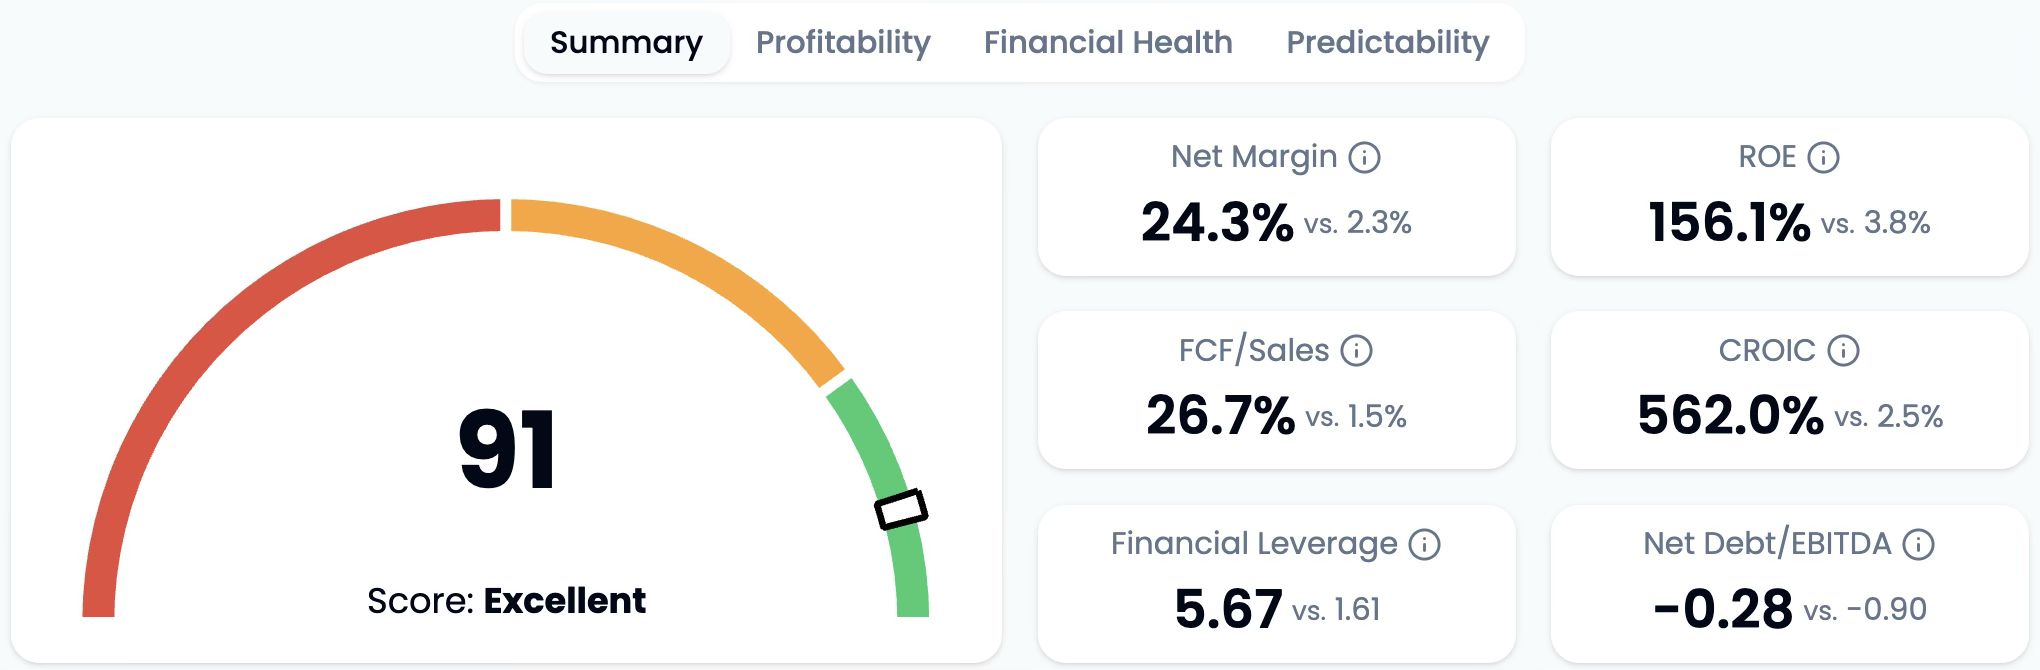
\includegraphics[width=0.8\textwidth]{images/tweenvest/quality score.png}
    \caption{Tweenvest's Quality Score}
    \label{fig:quality_score}
\end{figure}

\noindent After calculating all of this ratios, Tweenvest compares them to the sectors' median and interpolates each of them to create a single score for the ratio, then it aggregates them all using personalized weights to create the final Quality Score, which is then summarized and shown to the clients as seen in figure~\ref{fig:quality_score}. In the left we have the total score for the factor and in the right some of the most relevant ratios used to calculate it, comparing them to the sector. This format is consistent for all of the factors studied in this work.


\subsection{Growth}
\noindent The Growth Score evaluates a company's historical growth across multiple key metrics, and compares them to industry standards. This comprehensive approach ensures a balanced assessment of growth across different aspects of the business:

\subsubsection{Revenue \& Profitability Growth}
\begin{itemize}
    \item \textbf{Sales}: Measures growth in core revenue streams
    \item \textbf{\acrshort{ebitda}}: Captures growth in operational cash-generating ability before non-cash and financing impacts
    \item \textbf{Operating Income}: Reflects growth in profit from core business operations
    \item \textbf{Net Income}: Includes all income sources, showing overall profitability growth
\end{itemize}

\subsubsection{Cash Flow Growth}
\begin{itemize}
    \item \textbf{Operating Cash Flow}: Measures growth in cash generation from operations
    \item \textbf{Simple FCF}: A straightforward proxy for available cash after essential investments
    \item \textbf{Levered/Unlevered FCF}: Provide detailed views of free cash flow with and without debt impact
    \item \textbf{Owner Earnings}: Useful for volatile capex cases, emphasizing cash available to shareholders
\end{itemize}

\subsubsection{Capital Base Expansion}
\begin{itemize}
    \item \textbf{Total Assets}: Indicates expansion in overall asset base
    \item \textbf{Equity}: Reflects growth in shareholders' claim on the business
    \item \textbf{Tangible Book Value}: Highlights growth in physical net assets, excluding intangibles
    \item \textbf{Invested Capital}: Captures total capital being put to productive use
    \item \textbf{Capital Employed}: A broader measure of capital supporting business operations
\end{itemize}

\subsubsection{Per-Share Value Growth}
\begin{itemize}
    \item \textbf{Diluted \acrshort{eps}}: Tracks per-share earnings growth, accounting for dilution effects
    \item \textbf{Diluted Shares}: Included to track share count changes, ensuring EPS growth is not artificially inflated by buybacks or dilution
    \item \textbf{Ordinary \acrshort{dps}}: Tracks the growth of shareholder payouts, a proxy for confidence in future earnings
\end{itemize}

\vspace{0.5cm}
\noindent To compute the Growth Score, Tweenvest calculates 10-year, 5-year, and 3-year averages and then interpolates the growth rate to industry standards. This approach reinforces the long-term investment philosophy, giving lasting growing companies a better score.

\begin{figure}[H]
    \centering
    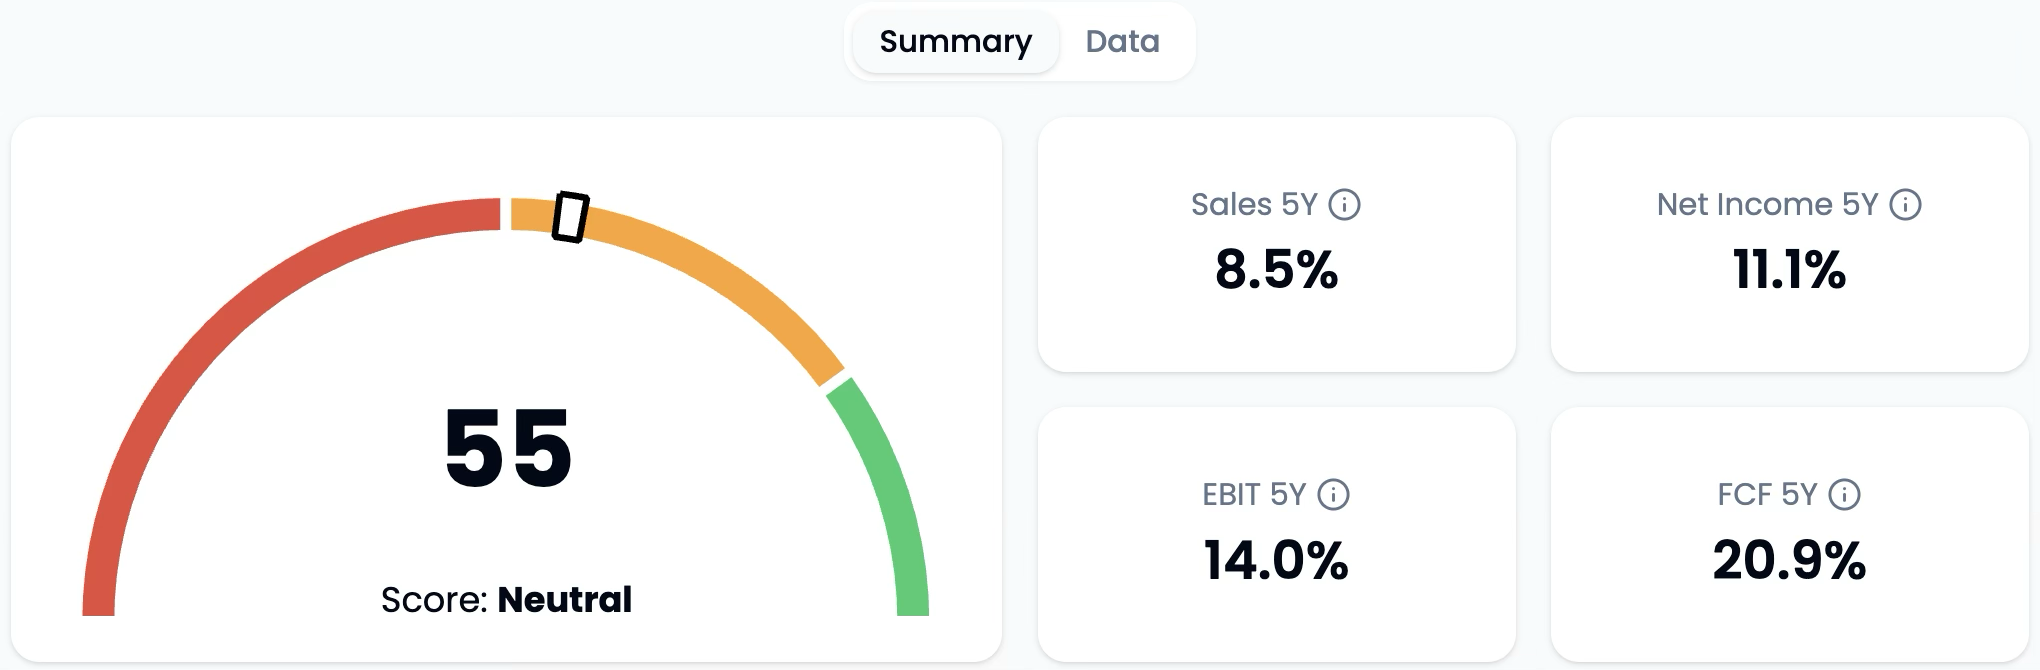
\includegraphics[width=0.8\textwidth]{images/tweenvest/growth score.png}
    \caption{Tweenvest's Growth Score}
    \label{fig:growth_score}
\end{figure}

\subsection{Value}
\noindent The Value Score measures how attractively a company is priced relative to fundamental multiples such as earnings, cash flow, sales, and dividends. This is critical for investors following value investing principles, where the goal is to buy quality companies for less than their intrinsic worth. The algorithm evaluates a series of valuation multiples—both price-based and enterprise value-based—and dividend yield.

\subsubsection{Price-Based Multiples}
\begin{itemize}
    \item \textbf{\acrshort{pe}}: Measures how much investors are willing to pay per dollar of earnings
    \item \textbf{\acrshort{ps}}: Useful when earnings are volatile; shows valuation relative to sales
    \item \textbf{\acrshort{pcf}}: Reflects valuation relative to cash-generating ability
    \item \textbf{\acrshort{pb}}: Especially relevant for asset-heavy sectors like banks or industrials
\end{itemize}

\subsubsection{Enterprise Value-Based Multiples}
\begin{itemize}
    \item \textbf{\acrshort{evsales}}: Indicates how much investors are willing to pay for each unit of revenue, providing a sense of overall company valuation relative to sales.
    \item \textbf{\acrshort{evebitda}}: Shows the value the market assigns to a company compared to its operating profitability before non-cash and financing items, useful for comparing companies with different capital structures.
    \item \textbf{\acrshort{evebit}}: Reflects the market value relative to operating earnings after depreciation and amortization, offering insight into core business profitability.
    \item \textbf{\acrshort{evfcf}}: Assesses how the market values a company in relation to the actual cash it generates, highlighting the ability to produce free cash flow for investors.
\end{itemize}

\subsubsection{Yield-Based Valuation}
\begin{itemize}
    \item \textbf{\acrshort{dividendyield}}: Measures the annual return on investment from dividends, expressed as a percentage of the current share price.
\end{itemize}

\vspace{0.5cm}
\noindent Each of these ratios is compared to multiple historical statistics and sector benchmarks to create individual scores and then average them.

\vspace{0.5cm}
\noindent \textbf{Note:}
\begin{itemize}
    \item \textit{\acrshort{marketcap} = Share Price × Total Outstanding Shares}
    \item \textit{Enterprise Value = \acrshort{marketcap}italization + Total Debt - Cash + Marketable Securities}
\end{itemize}

\begin{figure}[H]
    \centering
    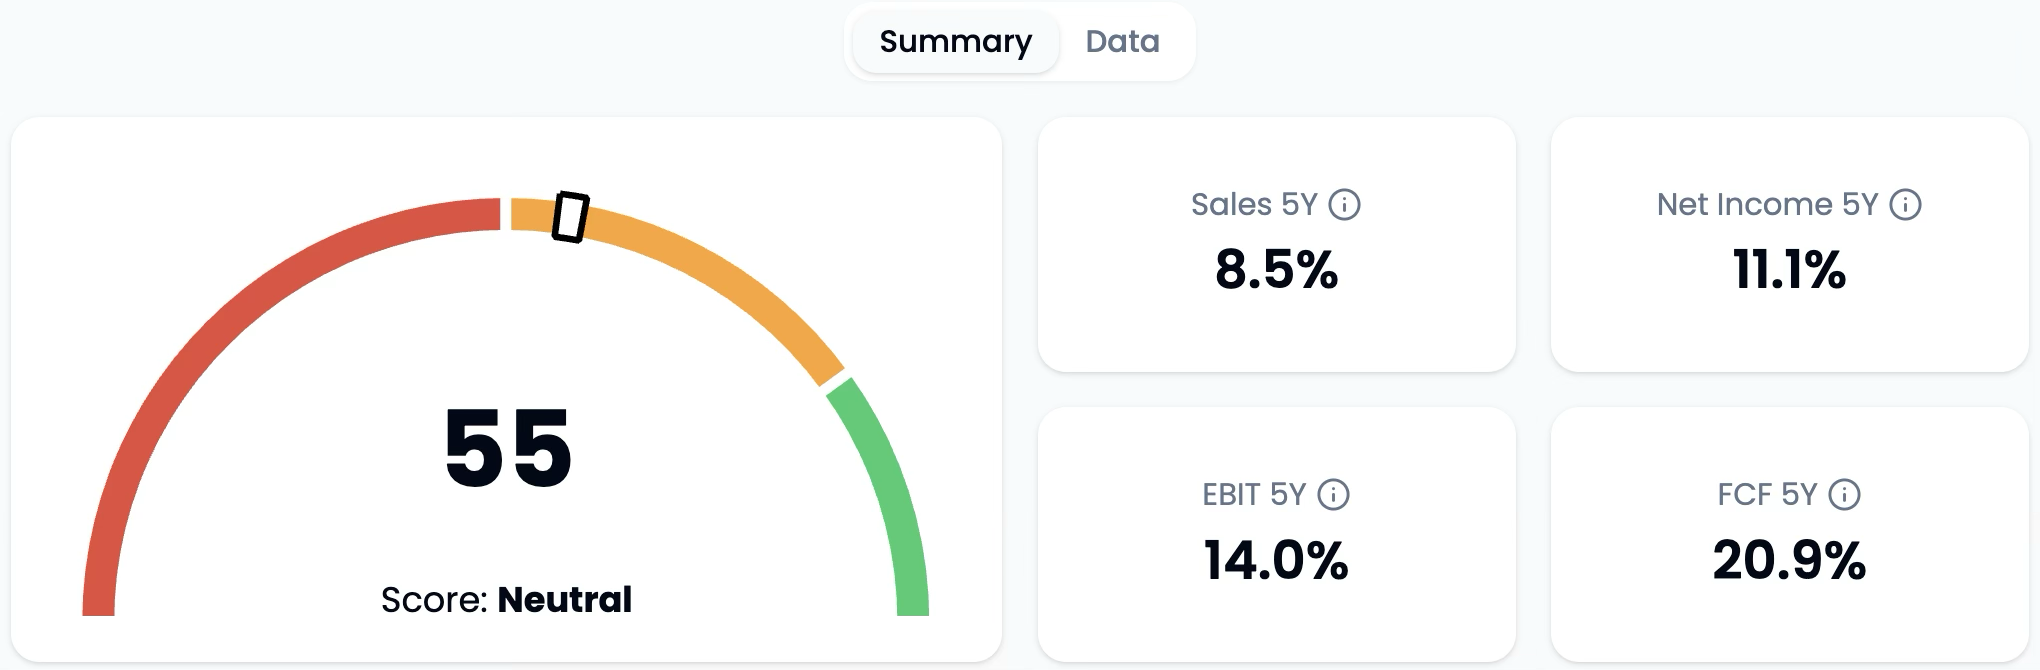
\includegraphics[width=0.8\textwidth]{images/tweenvest/value score.png}
    \caption{Tweenvest's Value Score}
    \label{fig:valuation_score}
\end{figure}


\subsection{Dividend}
\noindent When analyzing Tweenvest most common investors profile, we see a high tendency to income-focused and long-term investors using mainly dividends as their principal concern. Thats why the platform dedicated a full section to this topic. The Dividend Score measures the attractiveness, reliability, and growth potential of a company's dividend payments. It helps investors assess whether the dividend is both rewarding today and sustainable for tomorrow. To do so, the score was built from three primary components:

\subsubsection{Safety}
This part of the score is used to assess the sustainability of the dividend.
\begin{itemize}
    \item \textbf{\acrshort{payoutratioeps}}: Shows if dividends are covered by accounting earnings
    \item \textbf{\acrshort{payoutratiofcf}}: Shows if dividends are funded by real cash generation
    \item \textbf{\acrshort{payoutratioowner}}: A conservative test of sustainability, excluding \acrshort{capex}.
\end{itemize}

\subsubsection{Growth}
\noindent Measures how consistently and strongly the dividend has grown over time.
\begin{itemize}
    \item \textbf{Ordinary \acrshort{dps} \acrshort{cagr}}: 3-Year, 5-Year, 10-Year growth rates
\end{itemize}

\subsubsection{Yield}
\noindent This sub-score evaluates the attractiveness of the dividend today relative to the company's historical averages and sector benchmarks on \acrshort{dividendyield}.

\vspace{0.5cm}
\noindent These components are individually scored weighted and interpolated against industry benchmarks to form a composite score. 

\begin{figure}[H]
    \centering
    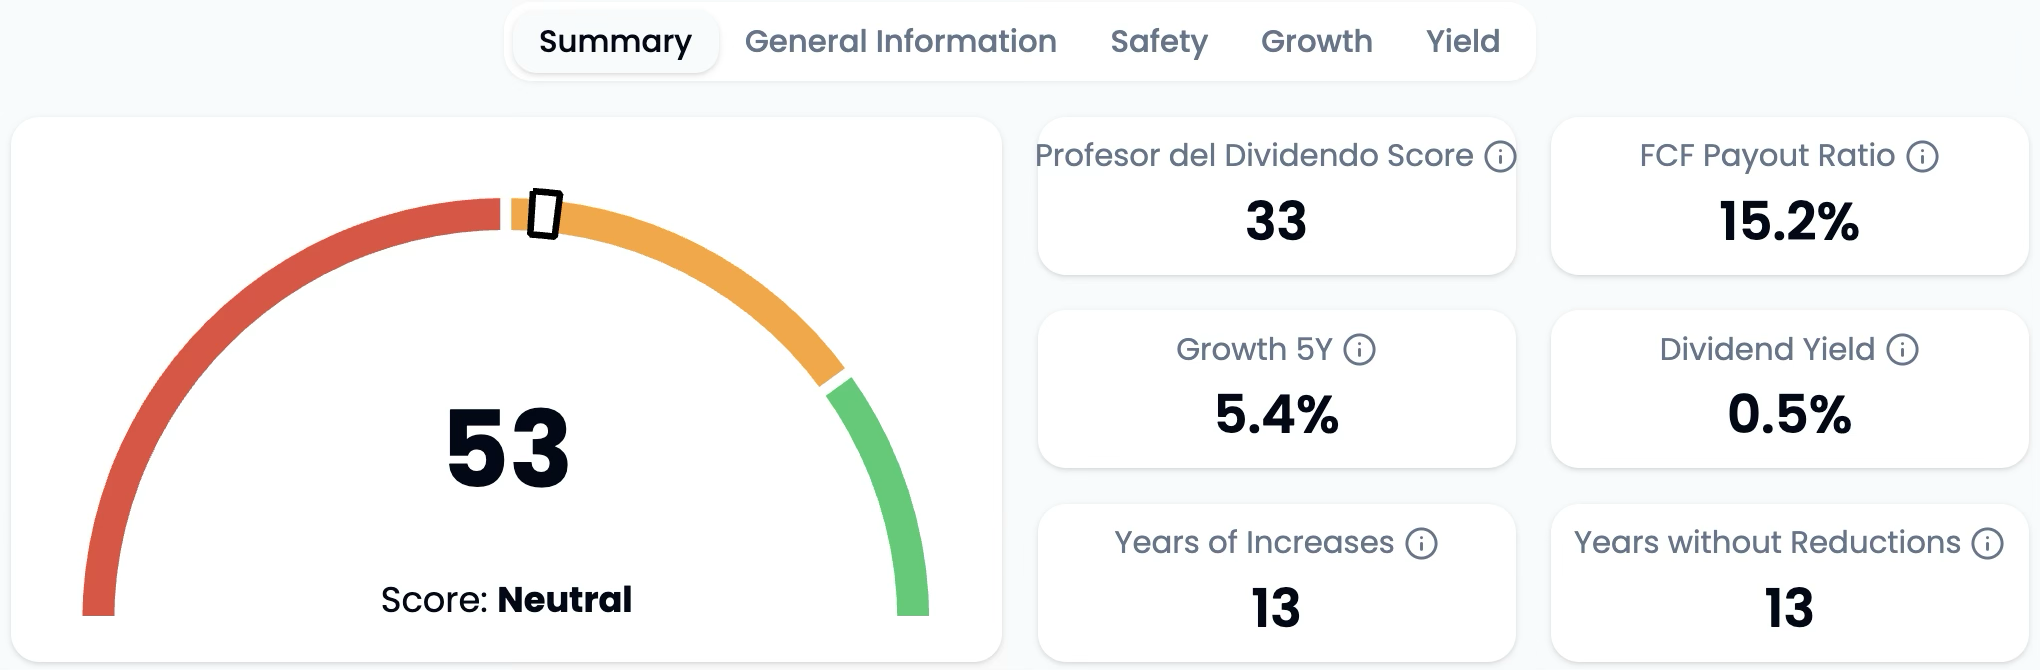
\includegraphics[width=0.8\textwidth]{images/tweenvest/dividend score.png}
    \caption{Tweenvest's Dividend Score}
    \label{fig:dividend_score}
\end{figure}

\noindent Finally, as seen in figure~\ref{fig:dividend_score}, the algorithm adjusts this score based on how many years the dividend has been maintained or increased, \textbf{rewarding consistency}.

\section{Code practices}
Since the code that needs to be changed is used in a production environment by Tweenvest, it is important to follow some \textit{``good practices''} to ensure the code is easy to understand, maintain, and to avoid introducing new bugs.

\begin{itemize}
  \item \textbf{Understanding and Documenting}: Before starting to work on the code, it is important to understand the codebase and the purpose of the code. For this, it is recommended to use some tools like flux diagrams, code comments, and documentation. As it will be shown later on.
  \item \textbf{Testing}: To ensure proper functionality, every function and class should have unit tests that cover all possible scenarios. These tests are run automatically by the \acrshort{ci/cd} pipeline.
  \item \textbf{Pair code review}: After completing the previous steps, the code undergoes a pair code review process, where at least one other team member reviews and approves the changes in \textit{Github} before merging into the main branch.
  \item \textbf{Logging}: After each feature is implemented, it is important to analyze the actual performance in the production environment by looking at its logs to check if the feature is working as expected, and to look for any possible optimizations to be made.
\end{itemize}

\section{Preprocessing}

After implementing the required code changes, the updated \acrshort{job}s are executed to extract the necessary information from Tweenvest’s systems. This process generates the raw dataset, which contains the historical scores alongside other financial and market variables required for the analysis. At this stage, the data is in its initial, unrefined form—directly pulled from various sources and potentially containing inconsistencies, missing values, or irrelevant records. Before it can be used for modeling, the dataset must be carefully inspected and processed to ensure it is coherent, complete, and aligned with the objectives of the study. This preprocessing stage is critical to avoid introducing bias, ensure the reliability of the results, and retain only the data that truly contributes to the evaluation of the scores.

\subsection{Data Consistency}

Since all of the data is coming from a data provider that uses \acrshort{ocr} as one of their tools whenever they do not have the data in a structured format, we need to be very restrictive with the data used. Also, as we mentioned before, some of the algorithms for calculating the scores use long-term data such as 10 year growths rates. This is one of the biggest \textbf{limitations to the study}: we will be missing the data of companies that stopped existing or that were acquired by other companies, if they did not exist for 10 or more years.

\vspace{0.5cm}
\noindent For inspecting the data we will be using Python as the main language, enhanced with: \textit{pandas}~\cite{pandas2025}, \textit{matplotlib}~\cite{matplotlib2025doc}, and \textit{seaborn}~\cite{seaborn2025}, which are powerful tools for data manipulation and analysis. The focus will be on the following aspects:
\begin{itemize}
  \item \textbf{Missing Values}: We need to check if there are any missing values in the data.
  \item \textbf{Data Distributions}: We need to make sure that the data is distributed in a way that is suitable for the modeling.
  \item \textbf{Variable Correlations}: We also have to see if there are any correlations between the variables. For this, we will use the correlation matrix defined as:
  \begin{equation}
    \rho_{X,Y} = \frac{\text{Cov}(X,Y)}{\sigma_X \sigma_Y}
  \end{equation}
  where \(\text{Cov}(X,Y)\) is the covariance between the variables \(X\) and \(Y\), \(\sigma_X\) is the standard deviation of \(X\), and \(\sigma_Y\) is the standard deviation of \(Y\). This matrix will be created with a custom heatmap function (see appendix~\ref{app:custom_functions}).
  \item \textbf{Data Patterns}: We need to check if there are any visible data patterns between the variables. To address this, we will use a custom \textit{\acrshort{pairplot}} function from \textit{seaborn}, which is a powerful tool for data visualization and exploration  depending on the type of variable (see appendix~\ref{app:custom_functions}).
\end{itemize}

\vspace{0.5cm}
\noindent Additionally, we decided to assign a value of 0 to all null Dividend scores, as a null value indicates that the company does not pay dividends. This choice was made to ensure that the Dividend score remains part of the analysis when evaluating its relevance to long-term profitability, rather than being excluded due to missing values.


% ############################### PREPROCESSING #######################
\subsection{Data Transformation}

To ensure a robust and well-performing model, it is often necessary to transform the data into a format more suitable for learning algorithms, with the obligatory condition of being able to revert it back to its original scale when needed. 

\vspace{0.5cm}
\noindent This step is particularly important because many components of machine learning models—such as the RBF kernel in Support Vector Machines or the regularization terms (L1 and L2) in linear models—implicitly assume that features are centered around zero and have comparable variances. Without this adjustment, features with significantly larger variances could dominate the optimization process, leading the model to underweight or ignore more informative but lower-variance features.

\subsubsection{Standard Scaler}
One of the predictive models we will use are neural networks, and for improving the training process of this type of models it is really important to standardize the data. We can easily use the \textit{StandardScaler} from the \textit{scikit-learn} library that transforms a feature \(x_i\) with the following formula:

\begin{equation}
z_i = \frac{x_i - \mu}{\sigma}
\end{equation}

\noindent where \(\mu\) is the mean of the feature and \(\sigma\) is its standard deviation. \textbf{This transformation is a very common practice}, and it results in a distribution with a mean of 0 and a standard deviation of 1.



\subsubsection{Gaussian Transformation}

In numerous modeling applications, having normally distributed features is advantageous. \textbf{Power transformations} represent a set of parametric, monotonic functions that are an extension of the Box-Cox transformation. They are designed to convert data from various distributions into approximately Gaussian distributions, thereby reducing variance fluctuations and decreasing distribution asymmetry. 

\vspace{0.5cm}
\noindent We decided to use the \textbf{Yeo-Johnson transformation} for the profits response variables, because it allows for negative values and it is reversible.

\begin{equation}
x_i^{(\lambda)} =
\begin{cases}
\frac{[{(x_i + 1)}^\lambda - 1]}{\lambda}, & \text{if } x_i \geq 0, \lambda \neq 0 \\
\ln(x_i + 1), & \text{if } x_i \geq 0, \lambda = 0 \\
-\frac{[{(-x_i + 1)}^{2 - \lambda} - 1]}{2 - \lambda}, & \text{if } x_i < 0, \lambda \neq 2 \\
-\ln(-x_i + 1), & \text{if } x_i < 0, \lambda = 2
\end{cases}
\end{equation}

\noindent Where \(\lambda\) is a power parameter that helps minimize the skewness of the data. And since we have already deleted extreme outliers, the final distribution should not be too distorted. In figure~\ref{fig:yeo-johnson}, we depict some examples of the transformation for different distributions:

\begin{figure}[H]
    \centering
    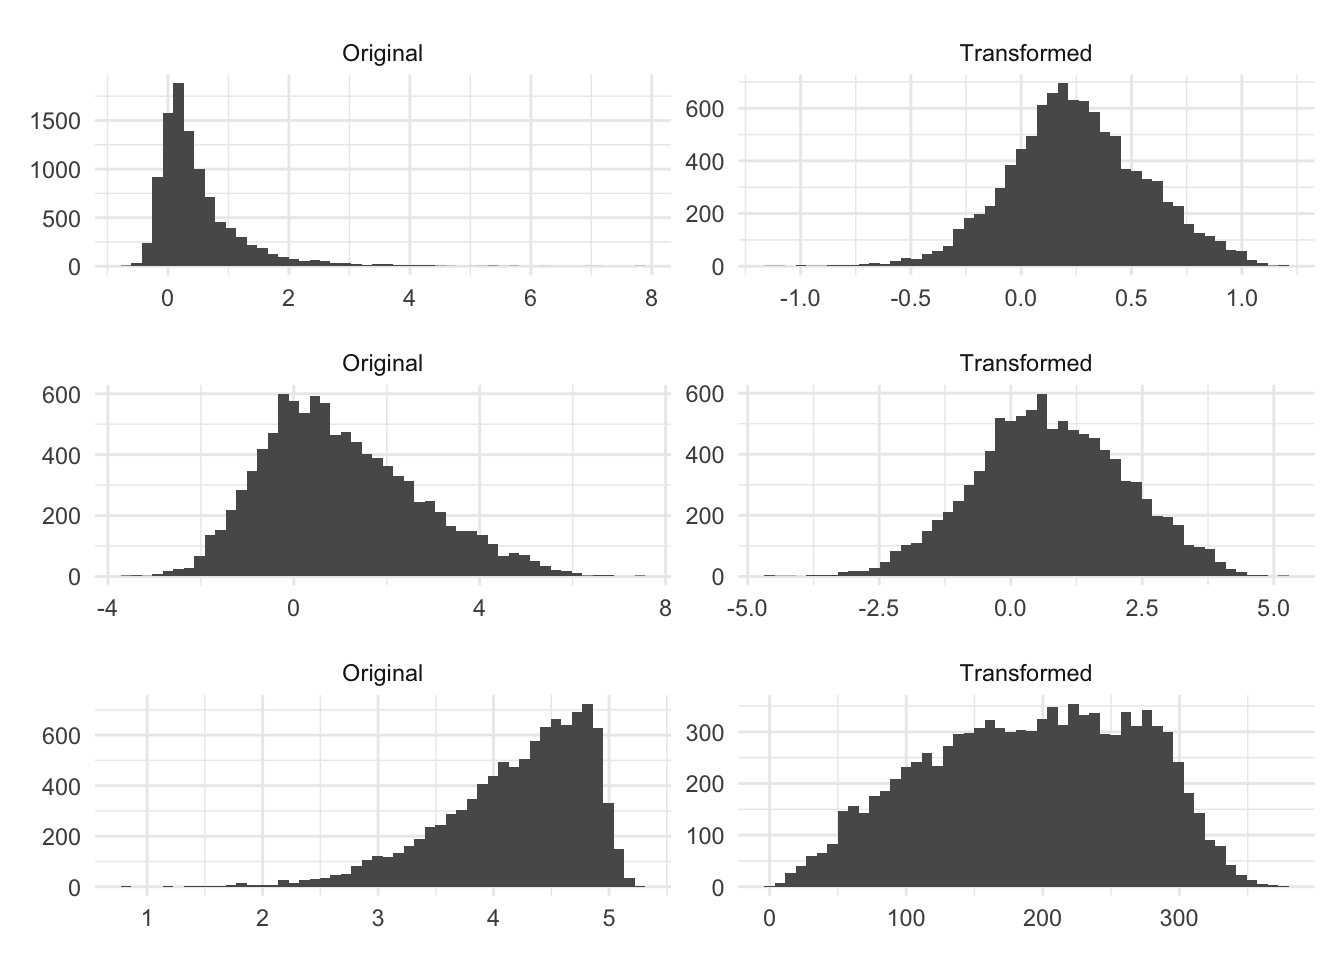
\includegraphics[width=0.5\textwidth]{images/code/transformations/yeo-johnson.png}
    \caption{Yeo-Johnson Transformations examples}
    \label{fig:yeo-johnson}
\end{figure}

\newpage
\section{Outlier Detection}
When we curate a database it is also necessary to consider anomalies. Anomalies are data patterns that have different data characteristics from normal
instances. The ability to detect anomalies has significant relevance since often provide critical and actionable information in many different contexts. For example, anomalies in credit card transactions could signify fraudulent use of
credit cards, or an unusual computer network traffic pattern could stand for an
unauthorized access.


\subsection{Inter Quartile Range}

Given a univariate dataset, the Interquartile Rule identifies outliers based on the \gls{iqr}. The steps are as follows:

\begin{enumerate}
    \item Compute the first quartile (\(Q_1\)), which is the 25th percentile of the data.
    \item Compute the third quartile (\(Q_3\)), which is the 75th percentile of the data.
    \item Calculate the interquartile range:
    \[
        \text{IQR} = Q_3 - Q_1
    \]
    \item Define the lower and upper bounds for non-outlier values following the 1.5 rule:
    \[
        \text{Lower bound} = Q_1 - 1.5 \times \text{IQR}
    \]
    \[
        \text{Upper bound} = Q_3 + 1.5 \times \text{IQR}
    \]
    \item Any data point \(x\) is considered an outlier if:
    \[
        x < \text{Lower bound} \quad \text{or} \quad x > \text{Upper bound}
    \]
\end{enumerate}

\noindent As we can see this is a very simple and intuitive method, but it has some limitations:

\begin{table}[H]
    \centering
    \begin{tabular}{|p{7cm}|p{7cm}|}
    \hline
    \textbf{Pros} & \textbf{Cons} \\
    \hline
    Simple to compute and interpret. & Not suitable for multivariate data with correlated features. \\
    \hline
    Non-parametric. & May misclassify values in skewed distributions as outliers. \\
    \hline
    Robust to extreme values, since it relies on percentiles rather than the mean. & Fixed multiplier is arbitrary and may need tuning for each dataset. \\
    \hline
    \end{tabular}
    \caption{Pros and Cons of the Interquartile Rule}
\end{table}

\noindent Even though this method is simple to compute and interpret, it is not suitable for multivariate data with correlated features, and that is where the rest of the methods come into play.

\subsection{Single Vector Machine}

\noindent The \gls{svm} represent a robust family of unsupervised learning algorithms that can be effectively adapted for anomaly detection tasks. This algorithm establishes itself on the premise that the majority of real-world data is inherently normal. Where the goal is to define a boundary encapsulating the normal instances in the feature space, thereby creating a region of familiarity. 

\vspace{0.5cm}
\noindent To capture the bases of the \textit{scikit-learn} implementation \cite{scikit2025oneclasssvm} used in this work, we can say that the main idea is to find a minimum volume sphere that contain all the training samples. This sphere, described by its center \(c\) and its radius \(r\), is obtained by solving the following optimization problem \cite{zineb2012simple}:
\begin{equation}
\min_{r,c} r^2 \quad \text{subject to} \quad \|\Phi(x_i) - c\|^2 \leq r^2 \quad \text{for} \quad i = 1, 2, \ldots, n
\end{equation}

\vspace{0.5cm}
\noindent This boundary is strategically positioned to maximize the margin around the normal data points, allowing for a clear delineation between what is considered ordinary and what may be deemed unusual. This emphasis on margin maximization is akin to creating a safety buffer around the normal instances, fortifying the model against the influence of potential outliers or anomalies. In summary, this method has the following characteristics:

\begin{table}[H]
    \centering
    \begin{tabular}{|p{7cm}|p{7cm}|}
        \hline
        \textbf{Pros} & \textbf{Cons} \\
            \hline
            Effective for high-dimensional data and complex boundaries. & Sensitive to the choice of kernel and hyperparameters (e.g., \(\nu\), \(\gamma\)). \\
            \hline
            Works well when the training set contains mostly or only normal instances. & Computationally intensive, especially on large datasets. \\
            \hline
            Can capture nonlinear patterns using kernels (e.g., RBF kernel). & Difficult to interpret or explain the decision function. \\
            \hline
            No need for labeled data from the outlier class. & -- \\
            \hline
            Solid theoretical foundation and widely supported in machine learning libraries. & -- \\
        \hline
    \end{tabular}
    \caption{Pros and Cons of One-Class \acrshort{svm} for Outlier Detection}
\end{table}
    
    
\subsection{Isolation Forest}

As we are seeing in this small fraction of outlier detection methodologies, most of the existing anomaly detection approaches are based on the premise of normal distributions, then identify anomalies as those that do not conform to the normal profile. But to solve this issue we can use the Isolation Forest algorithm, which is explained in the original paper \textcite{liu2012isolation}. The algorithm constructs multiple isolation binary-trees (iTrees) from the dataset, where anomalies are identified as data points that exhibit shorter average path lengths across these trees.

\vspace{0.5cm}
\noindent Lets consider a dataset \(X = \{x_1, \dots, x_n\}\) containing \(n\) points in \(d\)-dimensional space, and a subset \(X' \subset X\). An Isolation Tree (iTree) is constructed as follows:

\begin{itemize}
    \item Each node $T$ in the tree is either:
    \begin{itemize}
        \item An external node (leaf) with no children, or
        \item An internal node with exactly two children (\(T_l\) and \(T_r\)) and a test condition
    \end{itemize}
    \item The test condition at each internal node consists of:
    \begin{itemize}
        \item A randomly selected attribute \(q\)
        \item A split value \(p\)
        \item A test \(q < p\) that determines whether a point goes to \(T_l\) or \(T_r\)
    \end{itemize}
\end{itemize}

\noindent The tree construction process recursively partitions \(X'\) by randomly selecting attributes and split values until either:
\begin{itemize}
    \item The node contains only one instance, or
    \item All instances at the node have identical values
\end{itemize}
\begin{figure}[H]
    \centering
    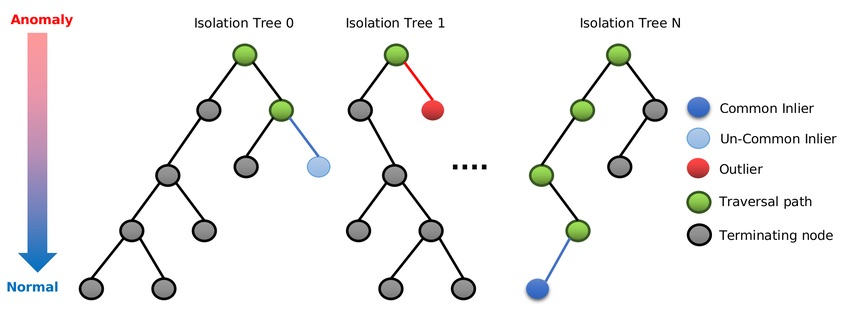
\includegraphics[width=0.8\textwidth]{images/code/outliers/IF.jpeg}
    \caption{Visualization of how \acrshort{if} works~\cite{dairi2022efficient}.}
    \label{fig:isolation_forest}
\end{figure}

\noindent As we can see in figure~\ref{fig:isolation_forest}, once the iTree is fully constructed, each point \(x_i \in X\) is isolated at a leaf node. The path length \(h(x_i)\) of a point \(x_i\) is defined as the number of edges traversed from the root to its leaf node. Points with shorter path lengths are considered more likely to be anomalies, as they require fewer splits to be isolated from the rest of the data.

\noindent This method works very good in most cases, but it has also its own limitations:

\begin{table}[H]
    \centering
    \begin{tabular}{p{7cm}p{7cm}}
    \toprule
    \textbf{Pros} & \textbf{Cons} \\
    \midrule
    Efficient and scalable to large datasets due to its tree-based structure. & Less effective for detecting local outliers in densely clustered regions. \\
    Non-parametric: does not assume any data distribution. & Performance can vary with the choice of parameters like number of estimators and subsample size. \\
    \hline
    Naturally handles high-dimensional data. & Not suitable for detecting subtle anomalies that closely resemble normal data. \\
    \hline
    Requires little preprocessing (no need for feature scaling). & -- \\
    \hline
    Robust to irrelevant features due to random sub-sampling. & -- \\
    \hline
    \end{tabular}
    \caption{Pros and Cons of the Isolation Forest Method for Outlier Detection}
\end{table}

\subsection{Local Outlier Factor}

Since we are looking at outliers from the perspective of correlations between the different response variables to see which companies do not behave naturally. We also checked on the \gls{lof} for being based on hyper-plane densities of data. The algorithm measures the local deviation of the density of a given sample with respect to its neighbors. It is local in that the anomaly score depends on how isolated the object is with respect to the surrounding neighborhood. More precisely, locality is given by k-nearest neighbors, whose distance is used to estimate the local density. By comparing the local density of a sample to the local densities of its neighbors, one can identify samples that have a substantially lower density than their neighbors. These are considered outliers. \cite{breunig2000lof}


\begin{table}[H]
    \centering
    \caption{Pros and Cons of the \acrshort{lof} Method}
    \begin{tabular}{|p{7cm}|p{7cm}|}
    \hline
    \textbf{Pros} & \textbf{Cons} \\
    \hline
    Can detect outliers relative to their local neighborhood, allowing it to identify context-specific anomalies. & \acrshort{lof} scores are relative and lack a universal interpretation threshold for outliers. \\
    \hline
    Effective in datasets with varying densities — unlike global methods, it can recognize outliers near dense clusters. & Sensitivity to parameter selection (e.g., number of neighbors) can affect performance and consistency. \\
    \hline
    Applicable in any domain where a dissimilarity measure is defined, not limited to vector spaces. & Can detect outliers patterns that could create a bias for models, because they do not belong to the normal distribution. \\
    \hline
    Works well across domains, such as network intrusion detection or classification tasks. & -- \\
    \hline
    Easily generalizable and adaptable for use in spatial data, temporal data, and network structures. & -- \\
    \hline
    \end{tabular}
\end{table}
    
\subsection{Multi-Criteria Outlier Detection}

There is a big controversy in the field about the best method to detect the outliers, since the results can vary a lot depending on the algorithm used.

\vspace{0.5cm}
\noindent So to attempt to fix this issue, after reading some aggregative methods such as \textcite{abro2020stacking}, we created a multi-criteria method that combines the results of the different methods to get a more robust result.

\begin{figure}[H]
    \centering
    \includegraphics[width=1\textwidth]{images/code/outliers/multimodal.png}
    \caption{\acrshort{multi} Schema}
    \label{fig:multimodal}
\end{figure}


\vspace{0.5cm}
\noindent As shown in the figure~\ref{fig:multimodal}, this starts by homogenizing the variables distribution with a common data transformation so they are more Normal, but to make sure that the final data is not being transformed we copy the original dataset earlier. After this, we use multiple methods to detect the different outliers and then we make the intersection between them to get the common outliers. By the end of this process we have tagged the original dataset rows, assuring that the data that will be excluded is only formed by \textit{"true outliers"}.

%TODO: maybe move this to the results section
% \vspace{0.5cm}
% \noindent We noticed that since this method is very restrictive, we had to set threshold multipliers to the original dataset to get the final outliers. So for example, a 20\% threshold would only exclude around 8\% of the original dataset because of the intersection of all the methods makes it very restrictive.

\subsubsection{Island Cases detector}

% TODO: explain the island detector.

When looking at the figure~\ref{fig:multimodal}, we can expect it to save different data points that are not common between all of the methods due to its intersection of \textit{true outliers}. This might be good for many classification tasks but when it comes to regression it can cause bias since there could be \textit{islands} --clusters-- of data that do not follow a normal distribution. Thats why we created a variation of the \acrshort{multi} method that should only keep the normal data but also saving those islands of data for further future analysis. Since those points do not have to be errors in the data,  they could show \textbf{extreme but consistent behavior} that should be modeled separately.

\begin{figure}[H]
    \centering
    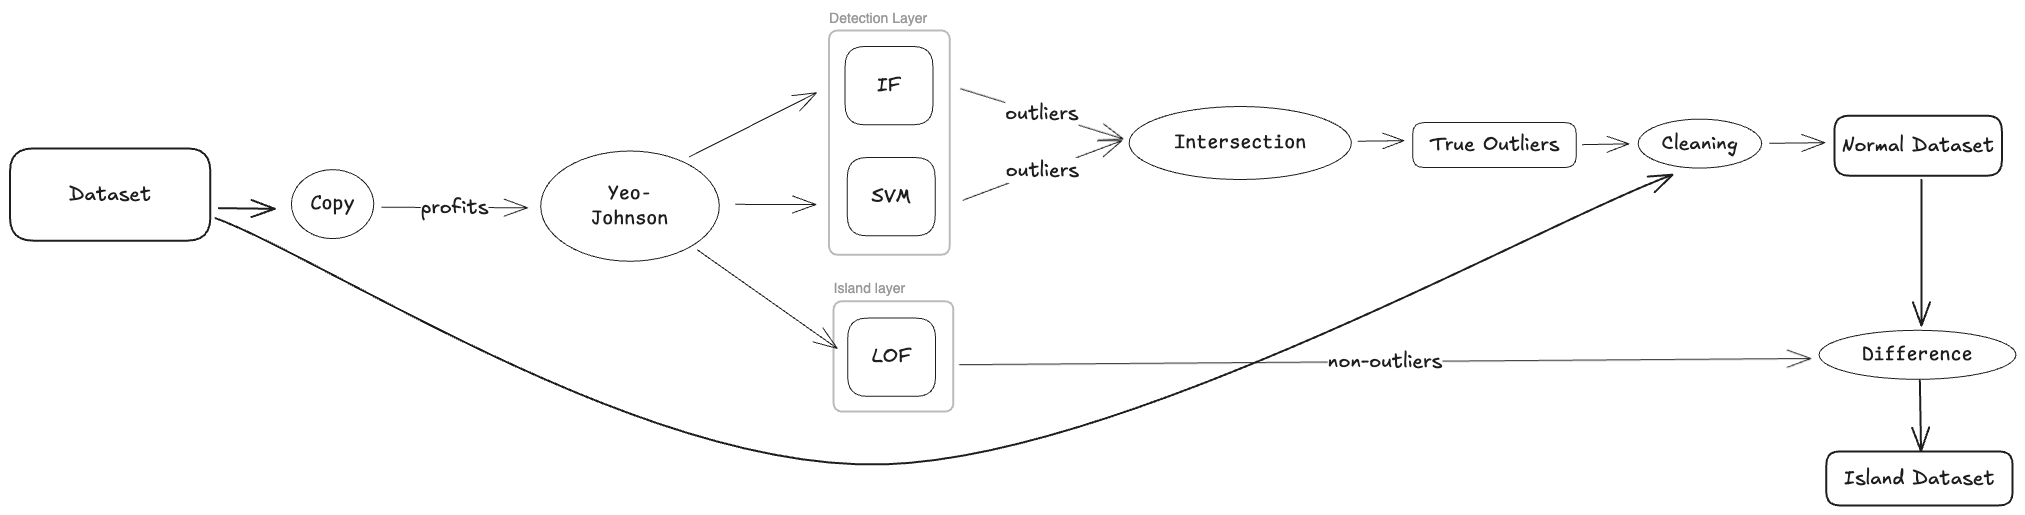
\includegraphics[width=1\textwidth]{images/code/outliers/Islands.png}
    \caption{\acrshort{islandcase} Schema}
    \label{fig:islands_of_outliers}
\end{figure}

% ############################### PREDICTIVE MODELS #######################
\section{Predictive Models}
The main objective of this thesis is to check if the scores have any relation with the future profits of the companies. For doing this in the most generalized way, instead of creating a portfolio following some subjective criteria on the scores, markets and other variables, we used predictive modeling to check for the actual relationships between the response variables and the explanatory ones.

\vspace{0.5cm}
\noindent Since the main objective is to check the relations between the profits and the scores, we used regression models to understand it those relationships. Starting with simple linear regression and then generalizing to non-linear models. And finally to test if we can also predict future profits we used \gls{nn}.


\subsection{Regression Models}

To create the econometrical models, we wanted to be able to understand the actual relationship between the response variables and the explanatory ones. For this we started with the creation of multiple regression models.

\subsubsection{Linear Regression}

As for the first models, we created a family of linear regression models (\(i \times j\)) for each factor i-return and j-score. These models include the interactions between the dummy variables and the j-score used in each model.

\begin{equation}
    \mu_{i,j} = \beta_0+\beta_1 \cdot S_j + 
\sum_{n=2}^{N}\beta_{n}\cdot D_n + S_j \cdot \sum_{m=N+1}^{M}\beta_{m}\cdot D_m
\end{equation}

\noindent where:
\begin{itemize}
    \item  \(R_{i,j} \sim \mathcal{N}(\mu_{i,j}, \sigma_{i,j}^2)\) is the return for each time horizon \(i\) and factor \(j\). So \(R_{i,j} = \mu_{i,j} + \varepsilon_{i,j}\) where \(\varepsilon_{i,j}\) is the error and \(\mu_{i,j}\) is the expected return.
    \item \(S_j\) is the score for each factor \(j\)
    \item \(D_{n,m}\) are the dummy variables for the industry and region, where \(D_{n,m} := I_k \cup G_l\)
    \item \(\beta\) are the coefficients that weight each variable.
\end{itemize}

\noindent For fitting the models, we also applied a \textbf{backward selection} to remove the variables that are not statistically significant, using the \textit{p-value} criterion \textbf{with a 20\% tolerance}. This threshold will be used for most of the analysis because in financial data it is harder to get high precisions.

\subsubsection{Generalized Additive Models}

Since the relationships between the variables are most likely non-linear, we also used the Generalized Additive Models (GAM) for the mentioned (\(i \times j\)) family to check if they are able to improve the performance, and also see if there are consistent patterns across the different time horizons.

\vspace{0.5cm}
\noindent With this analysis we could then let know Tweenvest what are the \textit{"best"} different scales for each score to better guide its users. Since right now --as it was shown in figures~\ref{fig:quality_score} to~\ref{fig:dividend_score}-- they are scaled from [0,50] as a bad score, (50, 80] as a good score, and (80, 100] as a great score. And this has not been tested yet.

\vspace{0.5cm}
\noindent According to \textcite{pygam2018}, GAMs are smooth semi-parametric models that can capture non-linear relationships between variables. They take the form:

\begin{equation}
    g(\mathbb{E}[y|X]) = \beta_0 + f_1(X_1) + f_2(X_2,X_3) + \dots + f_M(X_N)
\end{equation}

\noindent where:
\begin{itemize}
    \item \(X^T = [X_1, X_2, \dots, X_N]\) are the explanatory variables.
    \item \(y\) is the dependent variable, in our case the returns.
    \item \(g()\) is the link function that relates the predictor variables to the expected value of the dependent variable.
    \item \(f_m()\) are feature functions built using penalized B-splines, which automatically model non-linear relationships without requiring manual transformation of variables.
\end{itemize}

\noindent In our case, we used pyGAMs LinearGAM since the model gives a Normal error distribution, and an identity link. Using this library also gives us the possibility to differentiate between the different variable types:

\begin{itemize}
    \item \textbf{s(i) - Smooth Splines:} Standard smooth splines (cubic by default) for continuous variables like scores: \(f_m(X_m) = \sum_{j=1}^{k} \beta_{mj} B_j(X_m)\) where \(B_j\) are B-spline basis functions
    \item \textbf{f(i) - Factor Splines:} For categorical variables (sectors and regions): \(f_m(X_m) = \sum_{j=1}^{k} \beta_{mj} I_j(X_m)\) where \(I_j\) are indicator functions
    \item \textbf{te(i,j) - Tensor Splines:} For modeling non-linear interactions between variables: \(f_m(X_i, X_j) = \sum_{k=1}^{K_i} \sum_{l=1}^{K_j} \beta_{kl} B_k(X_i) B_l(X_j)\)
\end{itemize}

\noindent In figure~\ref{fig:splines_example} we can see an example of how GAMs can show the non-linear relationships between variables.
\begin{figure}[H]
    \centering
    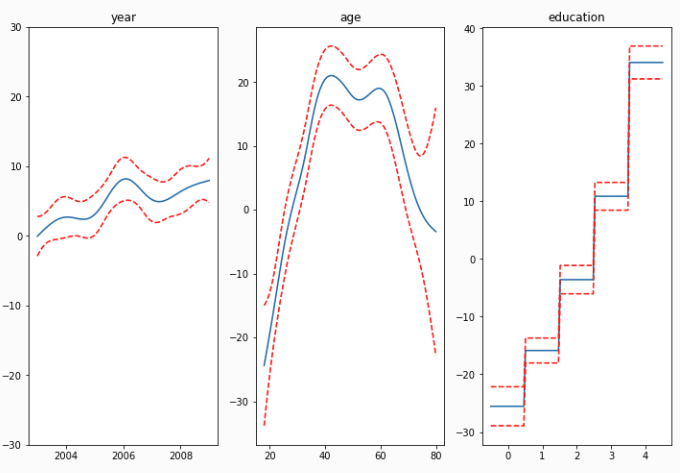
\includegraphics[width=1\textwidth]{images/code/descriptive analysis/gam/splines_example.png}
    \caption{pyGAM - Example of GAMs regression splines}
    \label{fig:splines_example}
\end{figure}

\subsection{Time Series}
In the stock market, the prices of the stocks are not independent from each other so as we will see with the descriptive analysis, they are correlated in the time series and they also have memory on past behavior of the company. This is what is known as \textbf{Momentum}, so companies that have a good past performance are more likely to have a good future performance, and vice versa. For this reason, we contemplated two possibilities:

\subsubsection{\Acrshort{arima} Models}
To take account the profit tendency, we implemented \acrshort{arima} models to improve the regression models performance by using the residues of the already fitted model:

\begin{equation}
    P_i = \hat{P_i} + {\varepsilon_i} \quad \longleftrightarrow \quad {\varepsilon_i} \sim ARIMA_i(p,d,q)
\end{equation}

\noindent The \acrshort{arima} model is defined as:

\begin{equation}
    \phi_i(B_i){(1 - B_i)}^{d_i} \varepsilon_i^t = \theta_i(B_i) \eta_i^t
    \end{equation}
    
    \noindent where for each \(i\) profit:
    \begin{itemize}
      \item \(\varepsilon_i^t\) is the residual at time \(t\).
      \item \(\eta_i^t\) is a white noise error term (innovation).
      \item \(B_i\) is the backshift operator, such that \(B \varepsilon_i^t = \varepsilon_i^{t-1}\).
      \item \(\phi_i(B) = 1 - \phi_{i1} B - \phi_{i2} B^2 - \dots - \phi_{ip} B^p\) is the autoregressive (AR) polynomial.
      \item \(\theta_i(B) = 1 + \theta_{i1} B + \theta_{i2} B^2 + \dots + \theta_{iq} B^q\) is the moving average (MA) polynomial.
      \item \(d_i\) is the order of differencing.
    \end{itemize}
    
\noindent But this approach supposed a \textit{big issue} that we will explain in the development section.

\subsubsection{Windowed Models}
So for trying to not fall into the same mistake and for capturing possible memory of the companies behavior in different aspects, we also implemented windowed models that used the last \(N\) scores statistical properties to predict future profits.

\vspace{0.5cm}
\noindent So for each score \(j\), we calculated the \textbf{average of the scores} over the last \(N\) periods. Let \(S_j^t\) be the score at time \(t\), then for a window of size \(N\):

\begin{equation}
    \bar{S}_j^N = \frac{1}{N} \sum_{i=t-N+1}^{t} S_j^i
\end{equation}

\noindent where:
\begin{itemize}
    \item \(\bar{S}_j^N\) is the average score over window \(N\) for score \(j\)
    \item \(N\) can be 3 months, 6 months, 1 year, or 2 years.
    \item \(t\) is the current time point
\end{itemize}

\noindent For adding also the deviation from the average, we also calculated the \textbf{standard deviation of the scores} over the same window:

\begin{equation}
    \sigma_j^N = \sqrt{\frac{1}{N} \sum_{i=t-N+1}^{t} (S_j^i - \bar{S}_j^N)^2}
\end{equation}

\noindent These statistical measures are used as additional features in our predictive models to capture the temporal behavior of each score.

\subsection{Neural Networks}
\acrshort{nn} are a class of machine learning models inspired by the structure and functioning of the human brain. They consist of an \textbf{input layer}, one or more \textbf{hidden layers}, and an \textbf{output layer}. The input layer receives the explanatory variables or regressors, which are then processed through the hidden layers where the model learns to represent and combine them in increasingly abstract ways. Within these hidden layers, nonlinear activation functions allow the network to capture complex, nonlinear relationships between variables—patterns that traditional linear regression or even more flexible methods such as \acrshort{gam} may fail to detect. Finally, the output layer produces the model’s prediction, which in this thesis corresponds to the expected profit or return over a given investment horizon.

\vspace{0.5cm}
\noindent The motivation for using \acrshort{nn} in this context lies in their ability to approximate highly complex functional relationships without requiring explicit specification of their form. Whereas linear or additive models are constrained by predefined assumptions about the shape of relationships, neural networks can automatically learn intricate dependencies and interactions among variables, making them particularly suitable for modeling financial data where nonlinearity and high-dimensional interactions are common. figure~\ref{fig:nn-basic-schema} illustrates the basic architecture of a neural network.

\vspace{0.5cm}
\begin{figure}[H]
    \centering
    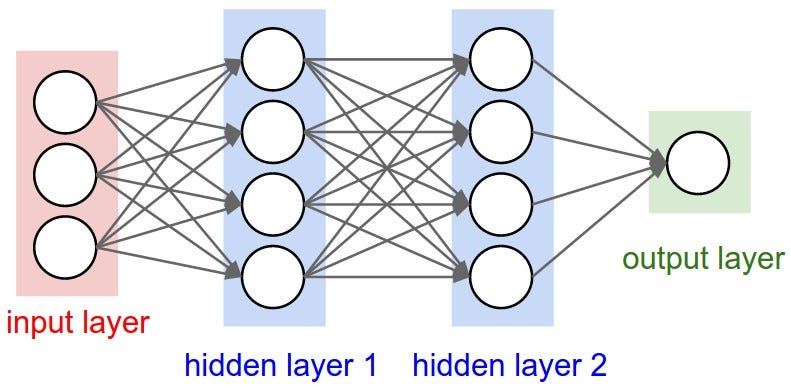
\includegraphics[width=1\textwidth]{images/code/neural_network/basic_schema.png}
    \caption{Simple Architecture of a \acrshort{nn}}
    \label{fig:nn-basic-schema}
\end{figure}

\noindent Finally, to test if we have enough information to model future profits, we will use two different approaches of different types of \acrshort{nn}: \textbf{regressors} and \textbf{classifiers}.

\subsubsection{Regressor Neural Networks}

\noindent
A \textbf{regressor neural network} is a type of artificial neural network specifically designed to predict continuous numerical values, rather than discrete categories. In the context of our analysis, these networks are trained to estimate future profit values based on a set of input features, such as historical scores and other relevant company data. For our implementation, we utilize the \textbf{MLPRegressor} from the \textit{scikit-learn} library~\cite{scikit2025mlpregressor}, which provides a flexible and efficient framework for building and training these models.

\subsubsection{Classifier Neural Networks}

\noindent To simplify the implementation, we are going to use two different quantification of the profits:

\begin{itemize}
    \item \textbf{Binary Classification:} In this approach, we partition the profit variable into two classes using the following rule:
    \begin{equation}
        y = 
        \begin{cases}
            0 & \text{if } P \leq 0 \\
            1 & \text{if } P > 0
        \end{cases}
    \end{equation}
    where \(P\) denotes the profit for a given time horizon, and \(y\) is the resulting binary class label.

    \item \textbf{Multi-class Classification:} Here we created different intervals of profits, using the average inflation rate and the S\&P 500 index as references--~\cite{global_inflation, sp500}.
    \begin{equation}
        y =
        \begin{cases}
            -3 & \text{if } P_a \leq -0.1 \\
            -2 & \text{if } -0.1 < P_a \leq -0.04 \\
            -1 & \text{if } -0.04 < P_a \leq 0 \\
             1 & \text{if } 0 < P_a \leq 0.04 \\
             2 & \text{if } 0.04 < P_a \leq 0.1 \\
             3 & \text{if } 0.1 < P_a
        \end{cases}
    \end{equation}
    \noindent Where \(P_a\) is the \textbf{annualized profit}, calculated as:
    \begin{equation}
        P_a = (1 + P)^{\frac{12}{n}} - 1
    \end{equation}
    \noindent Here, \(P\) is the total profit over a period of \(n\) months, and \(P_a\) is the equivalent annualized return.
\end{itemize}

\noindent And for building these \acrshort{nn} we will use the \textbf{MLPClassifier} from the \textit{scikit-learn} library~\cite{scikit2025mlpclassifier}, which provides a flexible and efficient framework for building and training these models. 

\subsubsection{Architecture Exploration}

\noindent Before building the models, we need to explore different architectures to find the best hyper-parameters for the models. In our case we are only going to explore the different hidden layers and the number of neurons in each layer, since the rest of the hyper-parameters are already being optimized by the library. To systematically explore the effect of the architectures, we will use the following configurations:

\begin{itemize}
    \item \textbf{Single hidden layer:} Networks with one hidden layer and varying width:
    \begin{itemize}
        \item (16), (32), (64), (128), (256), (512)
    \end{itemize}
    \item \textbf{Two hidden layers:} Networks with two hidden layers, both with decreasing and uniform widths:
    \begin{itemize}
        \item (64, 32), (128, 64), (256, 128), (512, 256), (128, 32), (256, 64)
        \item (32, 32), (64, 64), (128, 128), (256, 256)
    \end{itemize}
    \item \textbf{Three hidden layers:} Networks with three hidden layers, including both bottleneck and uniform structures:
    \begin{itemize}
        \item (128, 64, 32), (256, 128, 64), (512, 256, 128), (64, 32, 16), (256, 64, 16), (128, 64, 8)
        \item (128, 128, 128), (256, 256, 256)
    \end{itemize}
    \item \textbf{Four hidden layers:} Deeper networks with four hidden layers, both with gradually decreasing and large bottleneck structures:
    \begin{itemize}
        \item (512, 256, 128, 64), (256, 128, 64, 32), (128, 64, 32, 16), (64, 32, 16, 8), (1024, 512, 256, 128)
    \end{itemize}
    \item \textbf{Hard Bottlenecks:} Networks where the number of neurons sharply decreases in each subsequent layer:
    \begin{itemize}
        \item (256, 64, 16), (128, 32, 8), (512, 128, 32), (1024, 256, 64)
    \end{itemize}
\end{itemize}

\noindent
This comprehensive set of architectures allows us to compare the impact of network depth, width and \textit{bottlenecking} on predictive performance, and to identify the optimal configuration for each problem. So we should end up with a set of best architectures for each score and profits, depending on the \acrshort{nn} type.


\section{Back-testing}

In order to assess and compare the modeling techniques employed in this thesis, it is important to have a consistent criteria to evaluate them. Firstly we have to make clear that the main intent of this work is not to find the model that best predicts future profits, but to check whether the scores are correlated with the profits, and if so, how.

\subsection{Training and Testing}
\noindent
Knowing this, as we already explained, we will use the linear models and the \acrshort{gam} to check the correlations and the statistical significance of each variable. Then we will use the \acrshort{nn} to actually test the true predictability of the models. 

\begin{itemize}
    \item \textbf{Training:} We will use 80\% of the stocks of the dataset to train the models, excluding the last 4 months of each stock.
    \item \textbf{Testing:} When it comes to testing, we want to check the \acrshort{nn}-models in two different situations:
    \begin{itemize}
        \item \textbf{Unknown stocks:} Here we are using 20\% of the stocks left of the dataset, to see if just with the explanatory variables we can predict the future profits of those stocks.
        \item \textbf{Known stocks:} For these tests we will use 80\% of the stocks, that we used to train the models, but we will use the last 4 months of each stock to test if the models are able to predict when they already know past behavior of the stock.
    \end{itemize}
\end{itemize}

\subsection{Performance}
The first thing we need to see is if the models are able to detect any relationships between the co-variables and the response variable, and how accurate they are:
\begin{itemize}
    \item \textbf{Prediction capability:} we want to see if the models are able to predict the future profits, so we need to quantify the proportion of variance explained by the model. For this we will use:
    \begin{itemize}
        \item  \textbf{The coefficient of determination}, defined as:
        \begin{equation}
            R^2 = 1 - \frac{\sum_{i=1}^{n} {(y_i - \hat{y}_i)}^2}{\sum_{i=1}^{n} {(y_i - \bar{y})}^2}
        \end{equation}
        where \(y_i\) are the observed values, \(\hat{y}_i\) are the predicted values, and \(\bar{y}\) is the mean of the observed values.
        \item \textbf{The adjusted coefficient of determination}, to take into account the number of predictors in the model:
        \begin{equation}
            R^2_{adjusted} = 1 - \left(1 - R^2\right) \frac{n - 1}{n - p - 1}
        \end{equation}
        where \(n\) is the number of observations and \(p\) is the number of predictors. Since we are also using a \acrshort{nn} Classifier, we cannot use the same statistics as for regression.
        \item Thus, for prediction capability in classification, we will use the \textbf{F1 Score} from \textit{sklearn}, defined as:
        \begin{equation}
            F1 = 2 \cdot \frac{\text{Precision} \cdot \text{Recall}}{\text{Precision} + \text{Recall}}
        \end{equation}
        where \(\text{Precision} = \frac{TP}{TP + FP}\) and \(\text{Recall} = \frac{TP}{TP + FN}\), with \(TP\) being true positives, \(FP\) false positives, and \(FN\) false negatives.

        \vspace{0.05cm} This interprets as how many correct positive predictions the model makes relative to all positive predictions and actual positives, so a higher F1 score indicates better classification performance.
    \end{itemize}
    \item \textbf{Accuracy:} We also need to check on how much error the model is making when adjusted. For this we used:
    \begin{itemize}
        \item \textbf{The Mean Absolute Error}, defined as:
        \begin{equation}
            MAE = \frac{1}{n} \sum_{i=1}^{n} |y_i - \hat{y}_i|
        \end{equation}
        \item \textbf{The Root Mean Square Error}, for penalizing the larger errors or possible excess of outliers:
        \begin{equation}
            RMSE = \sqrt{\frac{1}{n} \sum_{i=1}^{n} {(y_i - \hat{y}_i)}^2}
        \end{equation}

        And again, for classification we decided to use:
        \item \textbf{Accuracy Score:} From \textit{sklearn} we used the accuracy score, which is defined as:
        \begin{equation}
            \text{Accuracy} = \frac{\text{Number of Correct Predictions}}{\text{Total Number of Predictions}}
        \end{equation}
        \item \textbf{Log Loss}: For mimicking the penalization for large errors we are using the log loss from \textit{sklearn}:
       \begin{equation} 
        \text{Log Loss} = -\frac{1}{n} \sum_{i=1}^{n} \sum_{j=1}^{m} y_{i,j} \log(\hat{y}_{i,j})
       \end{equation}
       where in this context, \(y_{i,j}\) represents the true class label, and \(\hat{y}_{i,j}\) represents the model's predicted probability for that class.
       
    \end{itemize}
\end{itemize}


\subsection{Consistency and Overfitting}
But a good performance does not mean that the models are explaining the behavior of the variables, they could be overfitting the data. To detect this, we need to check if the models reflect stable, interpretable patterns in the relationships between scores and the \textit{alpha}. For this, we will use the following criteria:
\begin{itemize}
    \item \textbf{Sign of coefficients:} We will check if the sign of the scores coefficients remains stable across different time horizons. This would tell us that the score behaves as expected. 
    \item \textbf{Shape of functions:} We will check if the shape of the spline functions of the GAMs remains stable across different time horizons. 
    \item \textbf{Number of significant variables:} We will check if the number of significant variables increases with the performance of the models, using the \textit{p-value} criterion.
\end{itemize}

\noindent And for the \acrshort{nn}, since we cannot access the internal structure of the models, we are going to use the \textbf{\gls{shap}} to check the importance of the variables in the predictions, and then use the same criteria for looking at the consistency of the variables in the models--~\textcite{lundberg2017unified}.

\subsection{Robustness of Results}
Even when the models perform well and show good consistency, it is essential to verify that their residuals resemble \textbf{white noise}. In the context of regression models—such as \acrshort{gam} and linear regression—this requirement stems from the assumptions underlying valid statistical inference. White noise residuals indicate that the model has successfully captured all systematic structure in the data, leaving only random, uncorrelated noise with constant variance. If residuals exhibit autocorrelation, trends, or heteroskedasticity, it suggests that relevant patterns remain unexplained, meaning the model may be misspecified or omitting important variables. 

\vspace{0.5cm}
\noindent Therefore, ensuring white noise residuals is a key diagnostic step to confirm that the relationships modeled are both complete and interpretable. This will be assessed through a combination of visual inspection and formal statistical tests \textcite{enders1948applied}. 

\begin{itemize}
    \item \textbf{Mean Value Test:} The mean of the residuals should be close to 0.
        \begin{itemize}
            \item \textbf{Distribution Plots:} Visualize the distribution of residuals to assess if the mean is centered at zero.
            \item \textbf{T-test:} Checks if the mean of the residuals is close to 0.
        \end{itemize}
    \item \textbf{Heteroskedasticity Tests:} The variance of the residuals should be constant across all time horizons.
        \begin{itemize}
            \item \textbf{Residuals vs Fitted Plots:} In a model with homoscedasticity (constant variance), the residuals should be randomly scattered around zero with a roughly constant spread.
            \item \textbf{White Test:} Checks for general forms of heteroskedasticity.
            \item \textbf{Breusch-Pagan Test:} Tests whether the variance of the errors depends on the values of the independent variables.
        \end{itemize}
    \item \textbf{Normality Tests:} The distribution of residuals should follow a Normal distribution.
        \begin{itemize}
            \item \textbf{\acrshort{qq} Plots:} Visual tool to compare the quantiles of the residuals to a normal distribution. If the data points in the \acrshort{qq} plot fall close to a straight diagonal line, it suggests that the data's distribution is similar to the theoretical distribution
            \item \textbf{Shapiro-Wilk Test:} Statistical test for normality.
            \item \textbf{Jarque-Bera Test:} Tests whether sample data have the skewness and kurtosis matching a normal distribution.
        \end{itemize}
    \item \textbf{Autocorrelation Test:} The errors should not be correlated with each other.
        \begin{itemize}
            \item \textbf{\gls{acf} and \gls{pacf} Plots:} Visualize the autocorrelation and partial autocorrelation of residuals.
            \item \textbf{Durbin-Watson Test:} Checks for the presence of autocorrelation in the residuals.
        \end{itemize}
\end{itemize}

\noindent \textit{Note: These residual diagnostics are not required for neural network (NN) models, as NNs do not rely on the same statistical assumptions as regression models.}

% ############################### DEVELOPMENT  ###############################
\chapter{Development}

\noindent This chapter details the practical implementation of the methodology described earlier, focusing on the steps taken to adapt Tweenvest’s infrastructure, create the datasets, and prepare them for analysis. The development phase bridges the conceptual framework with the operational execution, requiring modifications to the existing system architecture, the design of new data extraction jobs, and the deployment of solutions on dedicated servers. These tasks were carried out in close collaboration with Tweenvest, ensuring that all changes integrated seamlessly with the company’s production environment while maintaining data integrity and traceability.

\section{Architecture Enhancement}

\noindent At the current moment of beginning this work, Tweenvest kept a large \gls{db} of most of the needed information for creating the dataset. This included all of the price histories, historical currency multipliers to dollar, dividends payed per stock, etc. but when it came to the scores we had a traceability problem. For optimizing the costs and structure of the \acrshort{db}, Tweenvest chose to only save the latest score for each company and overwriting it each day when calculating the newest one, which led to the \textbf{first main task}.

\subsection{Updating Tweenvest Code}

After locating where the score calculators were called, we had to understand the code's architecture and the relationships between the different database models to see exactly what needs to be changed. Tweenvest uses \textit{Django} as the main backend's technology to handle a relational database with \textit{PostgreSQL}, this \acrshort{db} was chosen due to the nature of the financial data where information is related to another.

\vspace{0.5cm}
\noindent For handling all of the different technologies and environments, Tweenvest uses \textbf{\textcite{dockercompose2025}} to create a virtual machine that contains all of the needed dependencies to run the platform. This way, they have a consistent environment for developing, testing and deploying the code separately. So as we can see in figure~\ref{fig:general_architecture}, each of the components is running in a different container.

\begin{figure}[H]
    \centering
    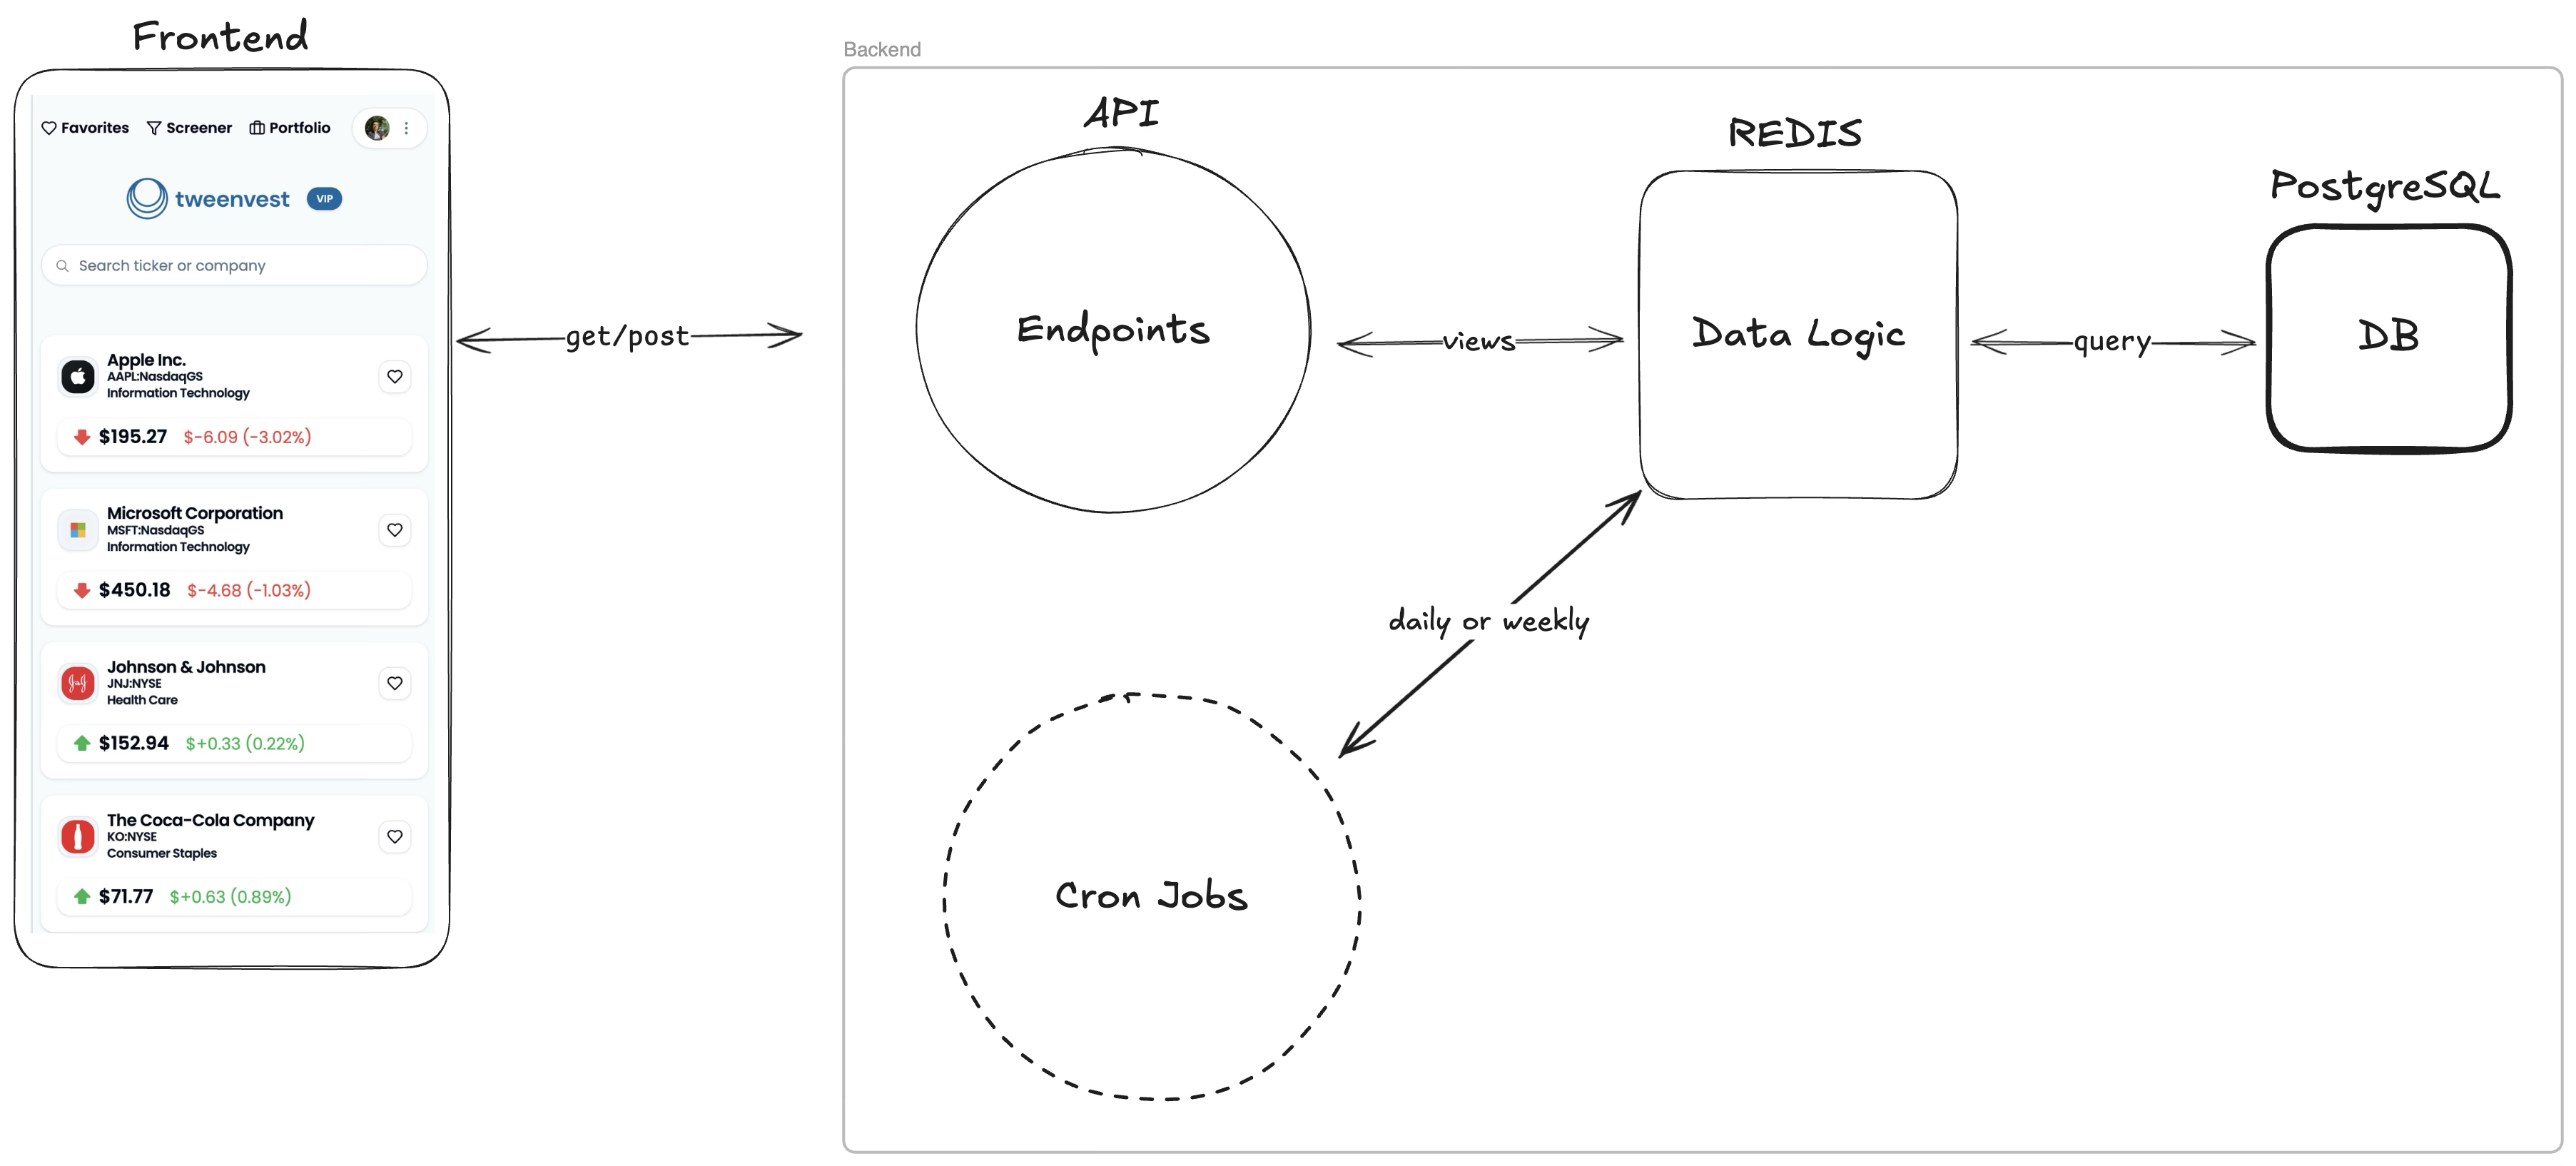
\includegraphics[width=1\textwidth]{images/tweenvest/general architecture.png}
    \caption{General Tweenvest's Architecture}
    \label{fig:general_architecture}
\end{figure}

\noindent Once we had a clear understanding of the architecture, we could look at the two different actions occurring at the same time: 
\begin{enumerate}
    \item Requests originating from user interactions.
    \item \acrshort{job}s that must be executed daily, weekly or at the moment, such as:
    \begin{itemize}
        \item Updating all financial information of the stocks.
        \item Performing necessary actions like sending emails to deliver authentication pins.
    \end{itemize}
\end{enumerate}

\noindent Since we were changing the data logic for calculating and storing historical data of the factor scores, we needed to assure that the systems capabilities do not exceed the platforms needs, and that the changes do not affect the normal calculation of the factor scores, so we had to look at the corresponding code of the factor scores.

\begin{figure}[H]
    \centering
    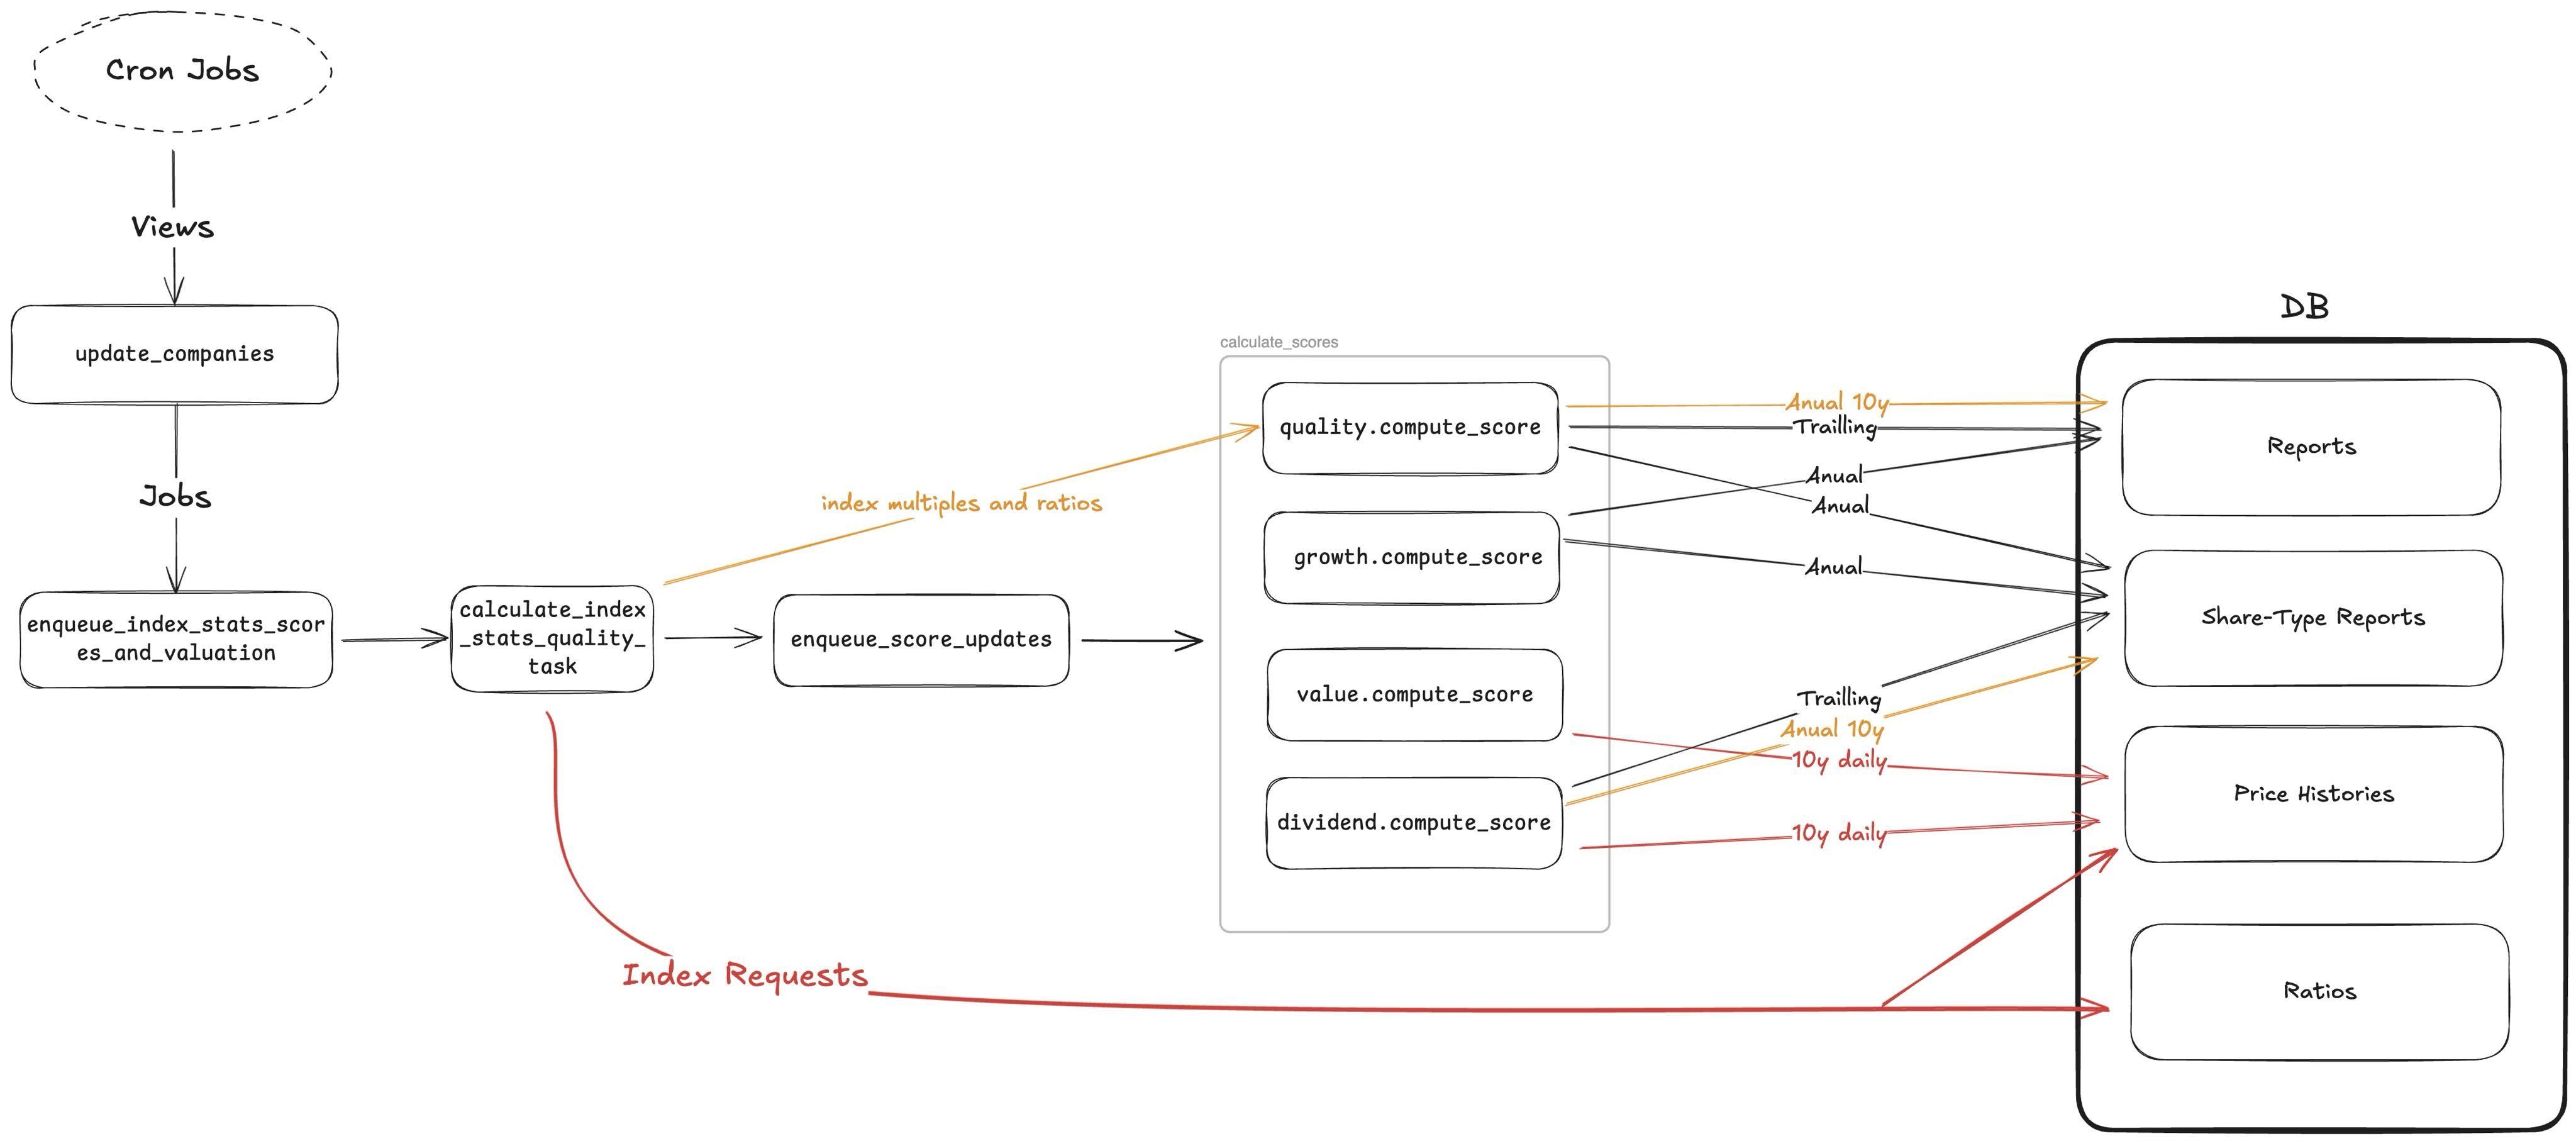
\includegraphics[width=1\textwidth]{images/tweenvest/scores schema.png}
    \caption{Scores Calculations Code Schema}
    \label{fig:scores_schema}
\end{figure}

\noindent The code integrates several methods and data-flows, so we created the schema shown in figure~\ref{fig:scores_schema} to simplify the logic behind several functions related to the calculations of each factor score. The scheduler triggers a request that is sent to the backend through the \textit{API} views, which then execute a series of functions responsible for calculating the scores for each factor. Seeing the chronology of the events, and the different queries to the \acrshort{db}, we quickly realized that we had to modify the queries to include an extra filter --\textit{calculation\_date}-- to get the models related to the score at any time, this way we could set it as ``today'' whenever we are calculating the present scores, not modifying the normal behavior of the system; while also having the ability to propagate the calculation to a specific past date.

\begin{figure}[H]
    \centering
    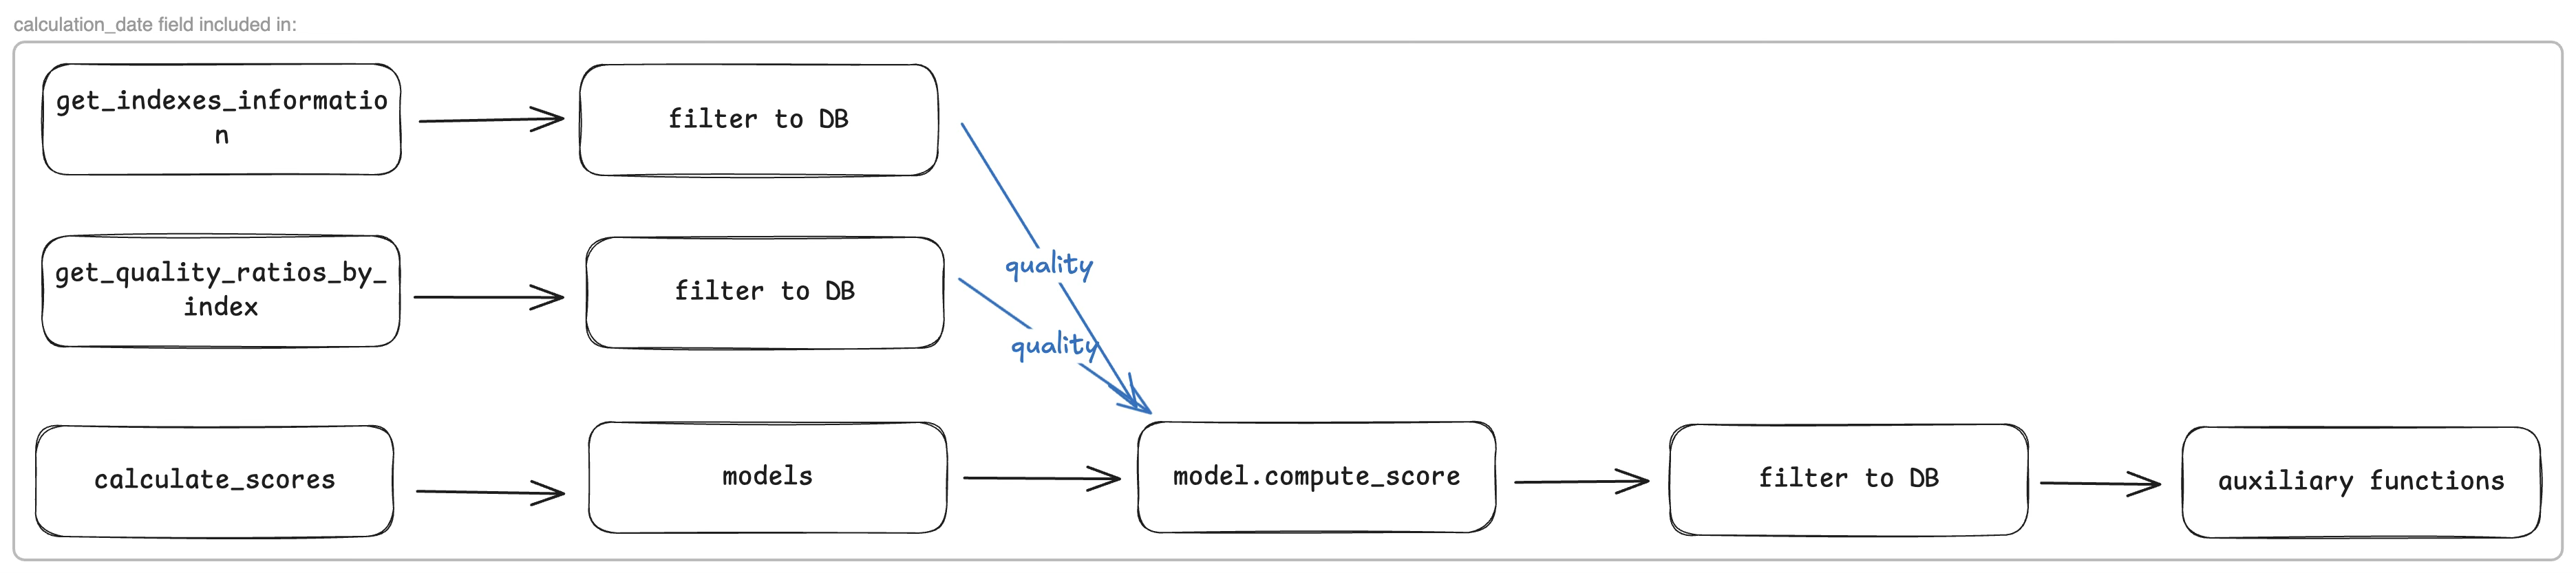
\includegraphics[width=1\textwidth]{images/tweenvest/Propagation Schema.png}
    \caption{\textit{calculation\_date} Field Propagation Schema}
    \label{fig:propagation_schema}
\end{figure}

\noindent For not adding redundant code, we had to inspect the propagation schema shown in figure~\ref{fig:propagation_schema} to determine the root changes from the main functions: \textit{calculate\_scores}, \textit{get\_indexes\_information} and \textit{get\_quality\_ratios\_by\_index}. These are the ones used by the production \textit{\acrshort{cron}} to calculate the factor scores daily, so for a normal function call we set the \textit{calculation\_date} to None and whenever we want to calculate the scores for a specific date we set it to the desired date. 

\vspace{0.5cm}
\noindent This helped us create very readable logic to adapt the filters to both scenarios, for example in the value score shown in Listing~\ref{lst:value_score_filtering}:

\begin{lstlisting}[language=Python, caption={Value Score Filtering}, label={lst:value_score_filtering}]
if calculation_date is None:
    calculation_date = date.today()
    filters = {
        "stock": stock,
        "date__gte": calculation_date - relativedelta(years=10),
    }
else:
    filters = {
        "stock": stock,
        "date__gte": calculation_date - relativedelta(years=10),
        "date__lte": calculation_date,
    }
phs = (
    PriceHistory.objects.filter(**filters)
)
\end{lstlisting}

\noindent So as we can observe, the main change for this part of the code was to add a date filter to get only data "lower than or equal" to the \textit{calculation\_date}. This may seem a bad approximation, but it has to be done this way due to the nature of the data: most of the financial data come from annual, semestral, and quarterly reports, except to the price history that is updated daily.

\vspace{0.5cm}
\noindent Along the way of analyzing the code's structure we made a small refactoring to simplify the legibility:
\begin{itemize}
    \item \textbf{Renaming functions} whenever they are internal methods or generic auxiliary methods called by different functions.
    \item \textbf{Externalizing mocking functions} that help create fake models and data for \textit{\acrshort{unittest}s}.
    \item \textbf{Homogenize the code's structure}, field types, to help with readability and keeping a standard order along the backend and frontend.
\end{itemize}

\noindent Another very important part of these updating procedure was to \textbf{adapt the \acrshort{unittest}s} to make sure that the original code still behaved as expected, \textbf{and creating new ones} to check that the changes calculated the factor scores properly.

\subsection{Designing new \acrshort{job}s}

Once all tests have passed and the team had approved the changes, the next step was to create new \acrshort{job}s to populate the current \acrshort{db} with the historic factor scores while maintaining the servers performance in normal levels. For this, we had to update a basic method, \textit{bulk\_create\_or\_update}, used many times through the whole codebase and add a new conditioning so it can handle conflicts depending if the models are empty or not. After reading the official Django \textcite{django2025queryset}, we saw that in the newest version available they had included the needed fields to its original method \textit{bulk\_create}, so \textbf{we had to update the \textit{Django} version} in our \textit{Docker} machine, making sure that it did not introduce any unwanted issues.

\vspace{0.5cm}
\noindent After this was implemented, we decided to create three different jobs for enqueueing the tasks and being able to separate the calculations. This way we could restart them in case something broke during the process (see appendix~\ref{app:historical_scores_job}). Also, we had to manage the server resources, so for assuring the platform's performance, we used the following hierarchy (see Listing~\ref{lst:tweenvest_production_workers_management}):
\begin{enumerate}
    \item Seven workers for primary daily jobs from different API data integration
    \item One dedicated worker for guaranteeing email sending, and 6 prioritized shared workers
    \item Four shared workers with lower priority, except for 1 which is set higher than email.
\end{enumerate}

\vspace{0.5cm}
\noindent A crucial part of this code was replicability, equal distribution through different sectors, and mostly to assure that the companies existed during enough time for the factor scores to calculate the 10 years averages.
\begin{figure}[H]
    \centering
    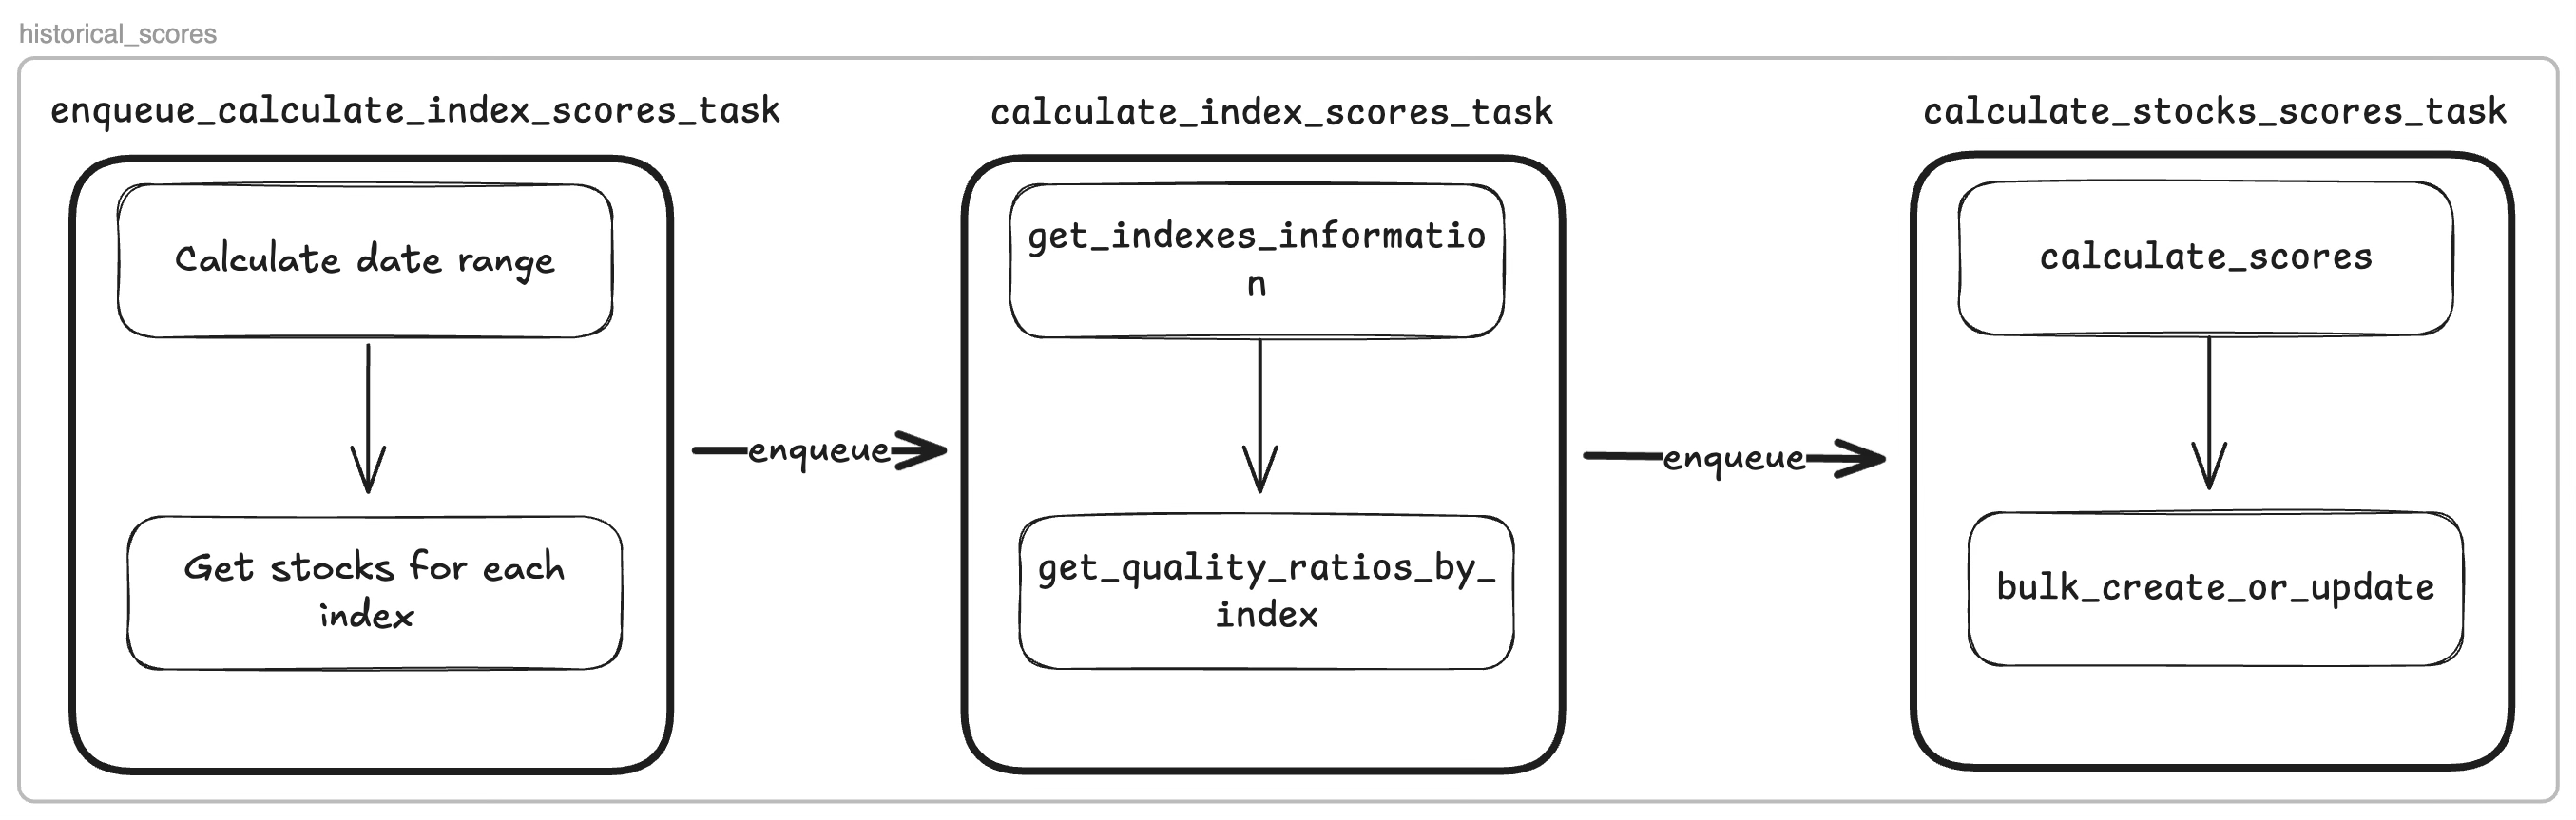
\includegraphics[width=1\textwidth]{images/tweenvest/Historical Jobs First Iteration.png}
    \caption{Historical Jobs First Iteration Schema}
    \label{fig:historical_jobs_first_iteration}
\end{figure}

\noindent We created the first jobs with the schema shown in figure~\ref{fig:historical_jobs_first_iteration}, and during the first small test it worked in local, but when tested with the production \acrshort{db} we started to see important issues with how the functions where designed due to the large amount of data being processed:
\begin{itemize}
    \item Passing incorrect arguments between jobs—such as entire lists of stock objects—led to the \acrshort{redis} \acrshort{db} reaching its maximum storage capacity.
    \item Jobs ran out of time, due to the large amount of data being processed.
\end{itemize}

\noindent We then changed the day range logic to enqueue a \textit{calculate\_index\_scores\_task} for each day, so the job did not have to calculate all of the index data for the dates all at once, as shown in figure~\ref{fig:historical_jobs_final_version}. Also, we modified the function \textit{args} to only uses models identifiers "id" to reduce the \acrshort{redis} memory used. The complete implementation of this job can be found in appendix~\ref{app:historical_scores_job}.

\begin{figure}[H]
    \centering
    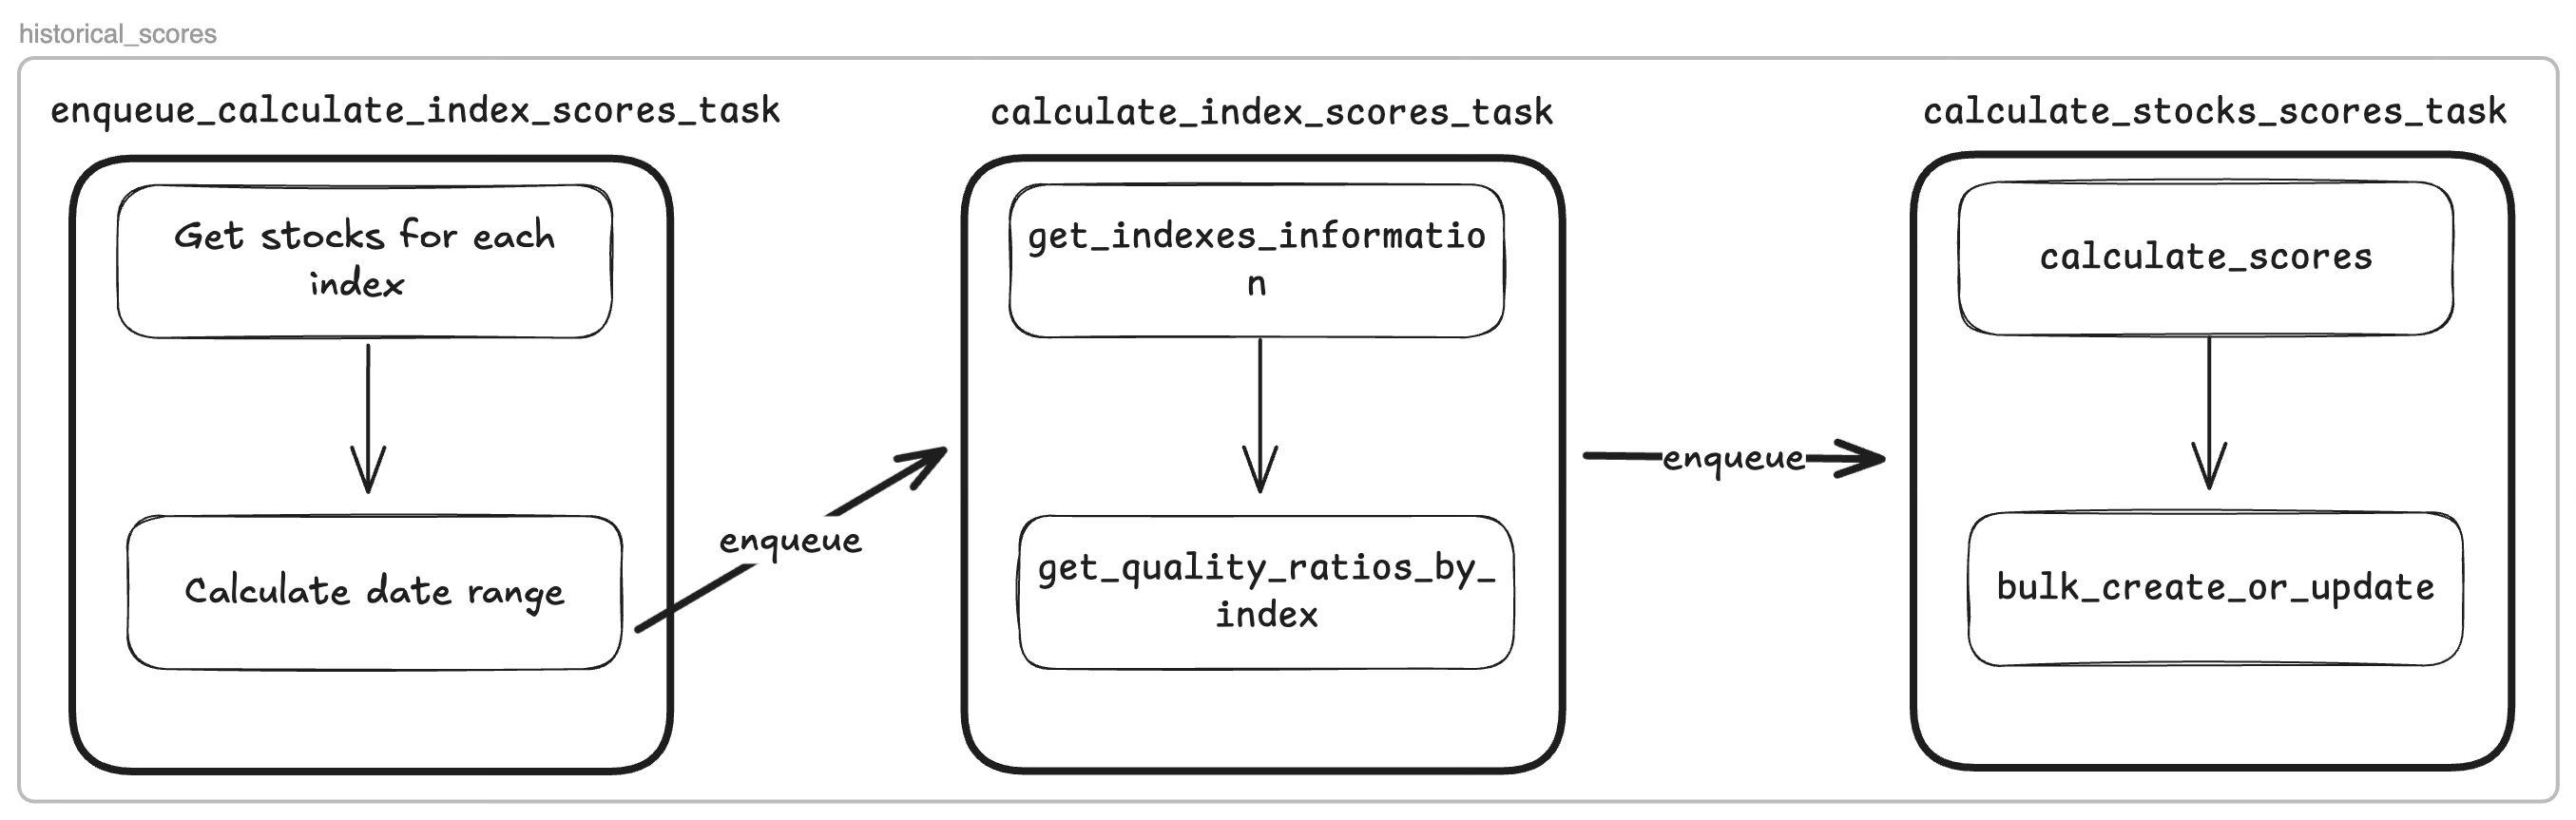
\includegraphics[width=1\textwidth]{images/tweenvest/Historical Jobs Final Version.png}
    \caption{Historical Jobs Final Version Schema}
    \label{fig:historical_jobs_final_version}
\end{figure}



\subsection{Telemetry Tracing}
Finally we had the functional jobs for calculating the scores, and ran the first calculation for a dataset of 1,500 stocks. After the first jobs finished we quickly realized that they were taking too much time to process, and saw a disproportionate amount of queries to the \acrshort{db} so we started a process to check on where was the bottleneck using telemetry tracing tools.

\vspace{0.5cm}
\noindent To do so, we had to inspect each method and function that was being used through the calculations of the factor scores. Luckily we had just recently implemented \textit{DataDog} which is a software that provides monitoring and analytics for applications and infrastructure, offering real-time metrics, event monitoring, and end-to-end tracing.

\vspace{0.5cm}
\noindent To apply the tracer, we simply had to add a specific \textit{\acrshort*{decorator}} before each method and set up the environment for being able to trace not only production launched jobs, but also development tests.

\vspace{0.5cm}
\noindent Here's an example of how the tracer was implemented in the quality score calculation:

\begin{lstlisting}[language=Python, caption=Telemetry Tracing Implementation, label={lst:telemetry_tracing_implementation}]
from opentelemetry import trace

tracer = trace.get_tracer(__name__)

@tracer.start_as_current_span("compute_quality_score")
def compute_quality_score(
    stock: "Stock",
    index_quality_ratios: Dict[str, IndexRatio],
    calculation_date: date | None,
) -> tuple[dict, dict]:
    ...
    return final_score
\end{lstlisting}

\noindent We then looked at the \textit{DataDog} dashboard and clearly saw an excess of queries to the \acrshort{db} when calculating each score, and tried to reduce them by looking for a simple fault in the logic of the queries. Similar issues were resolved before by adding a \textit{select\_related} in the queries. To clarify what this does, here is the definition with a simple use-case:

\vspace{0.5cm}
\noindent ``Returns a QuerySet that will follow foreign-key relationships, selecting additional related-object data when it executes its query. This is a performance booster which results in a single more complex query but means later use of foreign-key relationships will not require database queries.'' -- \textcite{django2025selectrelated}.

\vspace{0.5cm}
\noindent In Django, \textit{select\_related()} and \textit{prefetch\_related()} are designed to stop the deluge of database queries that are caused by accessing related objects. \textit{select\_related()} ``follows'' foreign-key relationships, selecting additional related-object data when it executes its query. \textit{prefetch\_related()} does a separate lookup for each relationship and does the ``joining'' in Python. So one uses \textit{select\_related} when the object that you're going to be selecting is a single object, so \textit{OneToOneField} or a \textit{ForeignKey}.

\vspace{0.5cm}
\noindent After numerous attempts to improve performance, we were forced to reconsider our approach and began analyzing the problem from a different perspective. It quickly became evident that we were operating on a small virtual machine (Table~\ref{tab:tweenvest_server_specs}) shared with the regular platform workload. Tweenvest's servers were not designed for high computational demand; rather, they were optimized for routine operations, where standard score calculations typically take between 3 to 4 hours. This setup works well under normal conditions, as calculations are performed after market hours and do not impact the user experience. However, it proved inadequate for our needs—specifically, processing data over five or more years within a reasonable timeframe, even when computing just one score per month.

\begin{table}[H]
    \centering
    \caption{Tweenvest Server Specifications}
    \begin{tabular}{|l|l|l|l|}
        \hline
        \textbf{VCPUS} & \textbf{RAM}  \\
        \hline
        2 & 4 GB  \\
        \hline
    \end{tabular}
    \label{tab:tweenvest_server_specs}
\end{table}


\subsection{Dedicated Server Deployment}
\noindent We made the decision to establish a dedicated server for this thesis, equipped with enhanced computational power to facilitate the calculations and data fitting.After evaluating several providers, we opted for Hetzner servers due to their exceptional quality-price ratio. The final setup consists of a dedicated server with the following specifications:

\begin{table}[H]
    \centering
    \caption{Hetzner Server Specifications}
    \begin{tabular}{|l|l|l|l|l|l|}
        \hline
        \textbf{VCPUS} & \textbf{RAM} & \textbf{SSD Storage} & \textbf{Extra Volume} \\
        \hline
        16 & 32 GB & 320 GB & 480 GB \\
        \hline
    \end{tabular}
    \label{tab:hetzner_server_specs}
\end{table}

\noindent Deploying the project in a scalable and reproducible environment involved several structured steps, encompassing server provisioning, secure remote access configuration using SSH, and initializing the containerized application deployment via Docker, with the application codebase managed through GitHub.

\vspace{0.5cm}  
\noindent After all of the setup was done, we saw an amazing \textbf{x100 performance improvement}, going from 15-minute calculation times for index statistics to 8 seconds. Finally, we could launch the factor scores historical calculations, so we created two subsets of 1,500 random companies each with the factor scores calculated for the 1st day of the month for the following periods: 2015-2020 and 2020-2025, which took a total of 3 hours.

\vspace{0.5cm}
\noindent Now that we had filled the \acrshort{db} with the necessary factor scores for the study, we ran a big calculation to get all of the possible factor scores for the +100,000 companies, which took several days.

\section{Dataset Creation}

\subsection{Aggregating the data}

For being able to continue, we needed to create the final dataset with all the necessary data for later on doing the analysis and developing the predictive models, so we created a simple algorithm with this logic:

\begin{figure}[H]
    \centering
    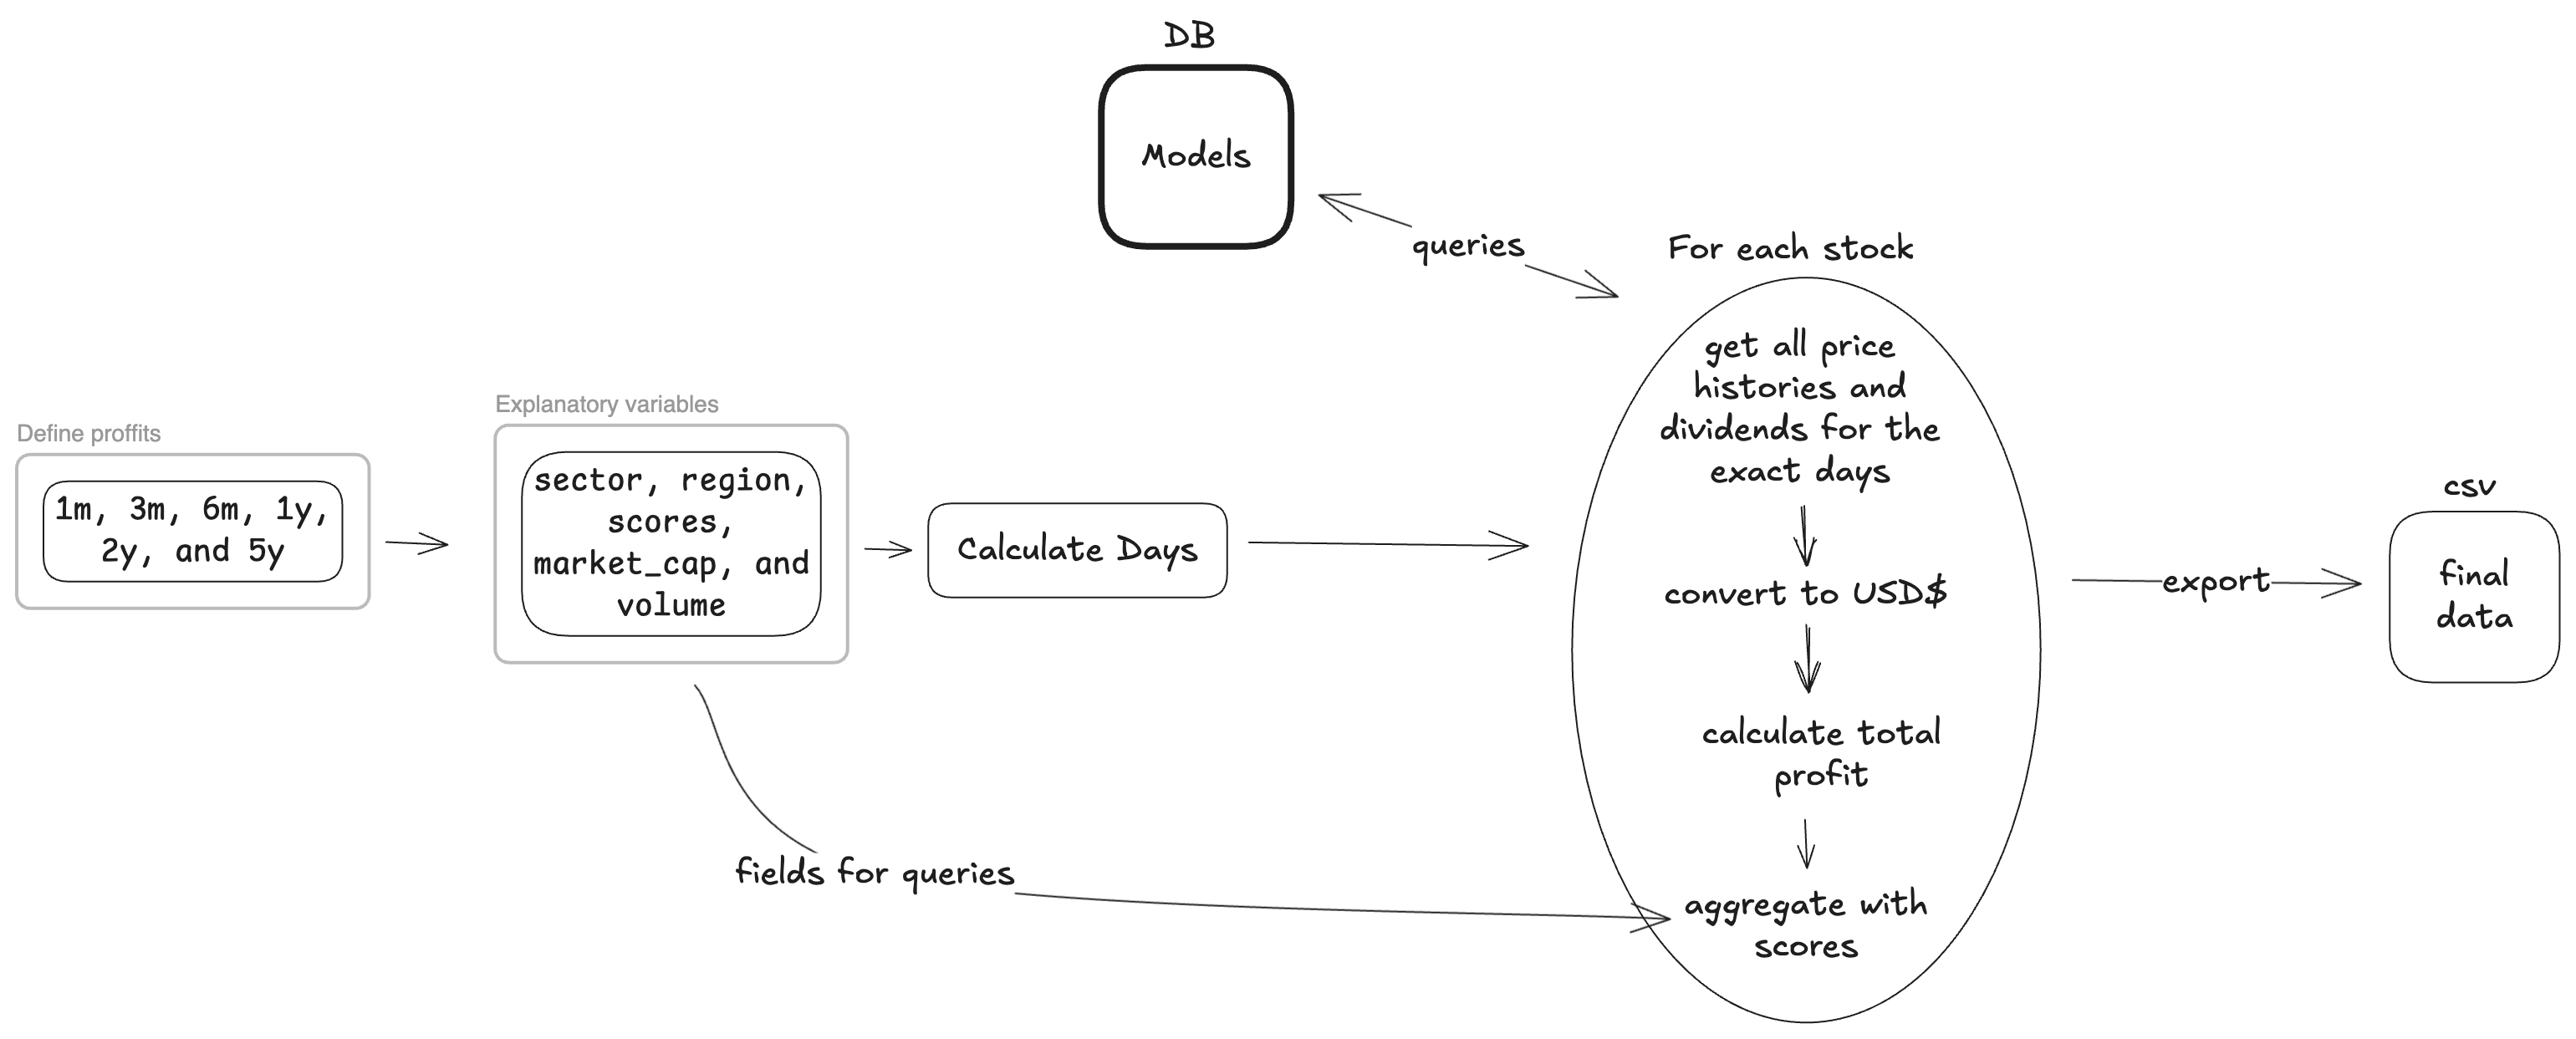
\includegraphics[width=0.8\textwidth]{images/tweenvest/First Data Aggregation Schema.png}
    \caption{First Data Aggregation Schema}
    \label{fig:first_data_aggregation_schema}
\end{figure}

\noindent Once we had the final csv file we noticed that we had too many empty values for profits, the problem was that some of the days calculated were empty for a specific company, so there was no price history for them. Since companies belong to multiple countries, different holidays could be causing another major loss in the information. To fix this in a general way \textbf{we implemented an internal method} for estimating price histories when they did not exist for the wanted date. The complete implementation of this data export and price estimation process can be found in appendix~\ref{app:data_export_job}.

\begin{figure}[H]
    \centering
    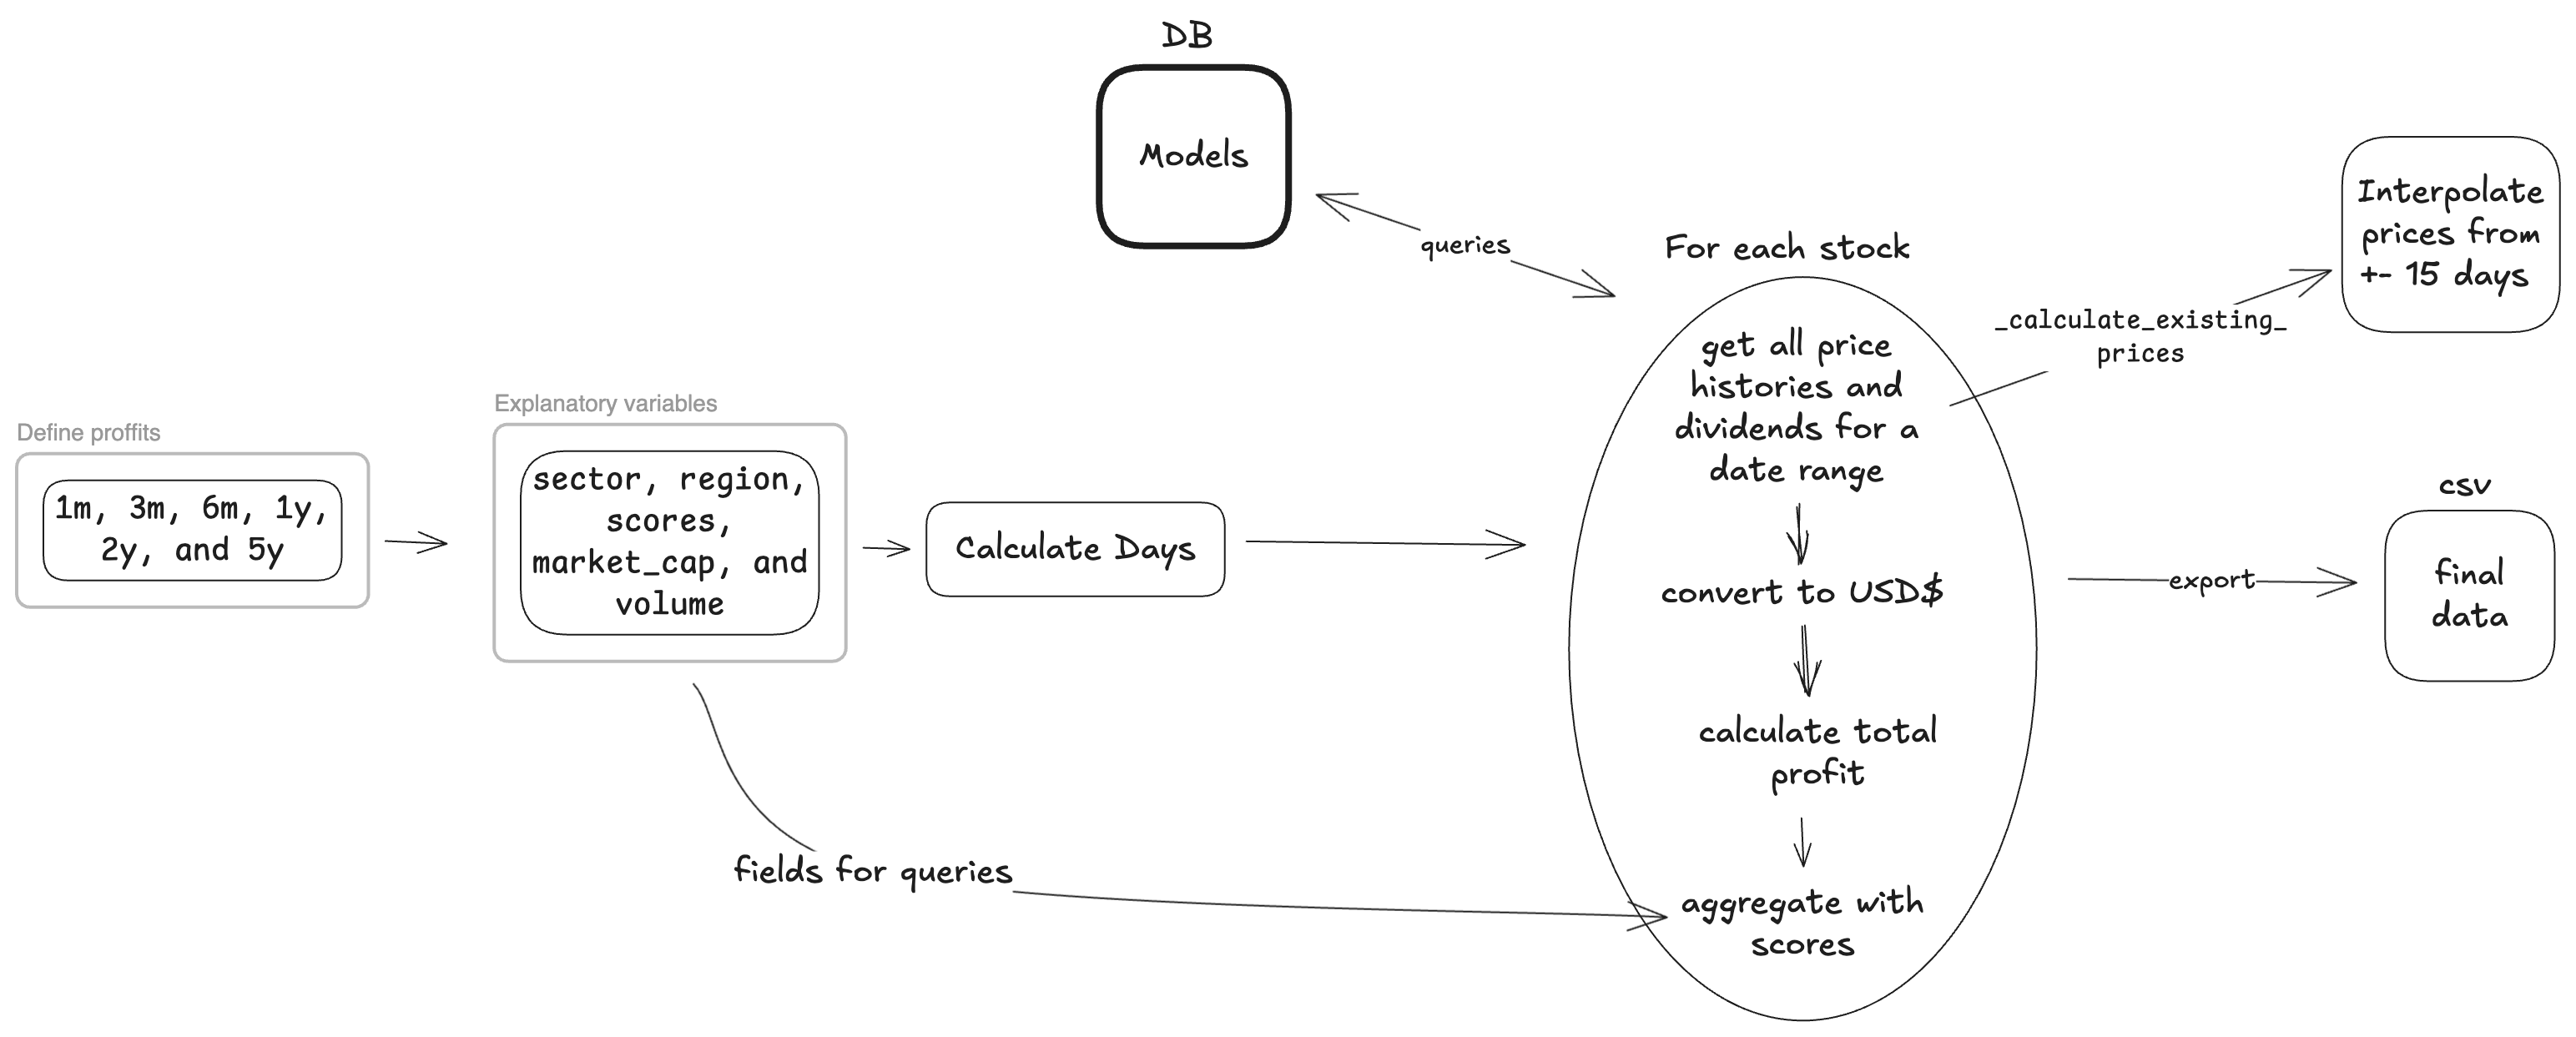
\includegraphics[width=0.8\textwidth]{images/tweenvest/Final Data Aggregation Schema.png}
    \caption{Final Data Aggregation Schema}
    \label{fig:final_data_aggregation_schema}
\end{figure}

\noindent By looking at the figure~\ref{fig:final_data_aggregation_schema} we can see that we are interpolating those price histories. Since we are only looking for long term profitabilities, we can \textbf{approximate the price} on a day $x$ by interpolating the price on $x-y$ and $x+z$, weighted by how close they are to the original day $x$, with a maximum distance from $x$ of 15 days. This significantly reduced the amount of missing values.

\subsection{Datasets Construction}

For this study, we have attacked the objectives from multiple perspectives. First we are making a descriptive analysis to understand the data, and then we are proposing different models to see if there are any relationships between the scores factors and long term profitabilities. Thats why when creating the datasets, we made two different approaches to have more information for the analysis:

\begin{figure}[H]
    \begin{minipage}{0.48\textwidth}
        \centering
        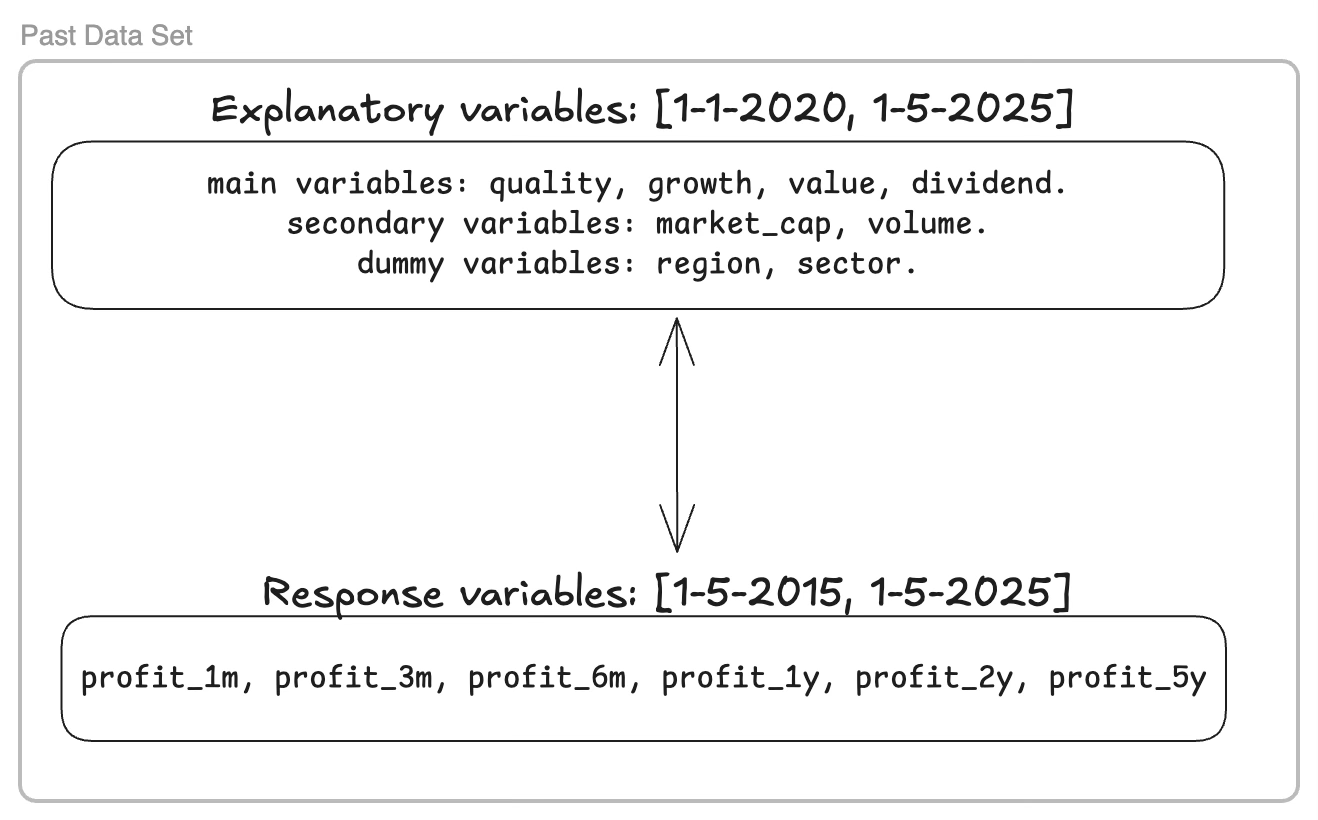
\includegraphics[width=\textwidth]{images/tweenvest/Past Dataset variables relations.png}
        \caption{Past Dataset}
        \label{fig:past_dataset}
    \end{minipage}
    \hfill
    \begin{minipage}{0.48\textwidth}
        \centering
        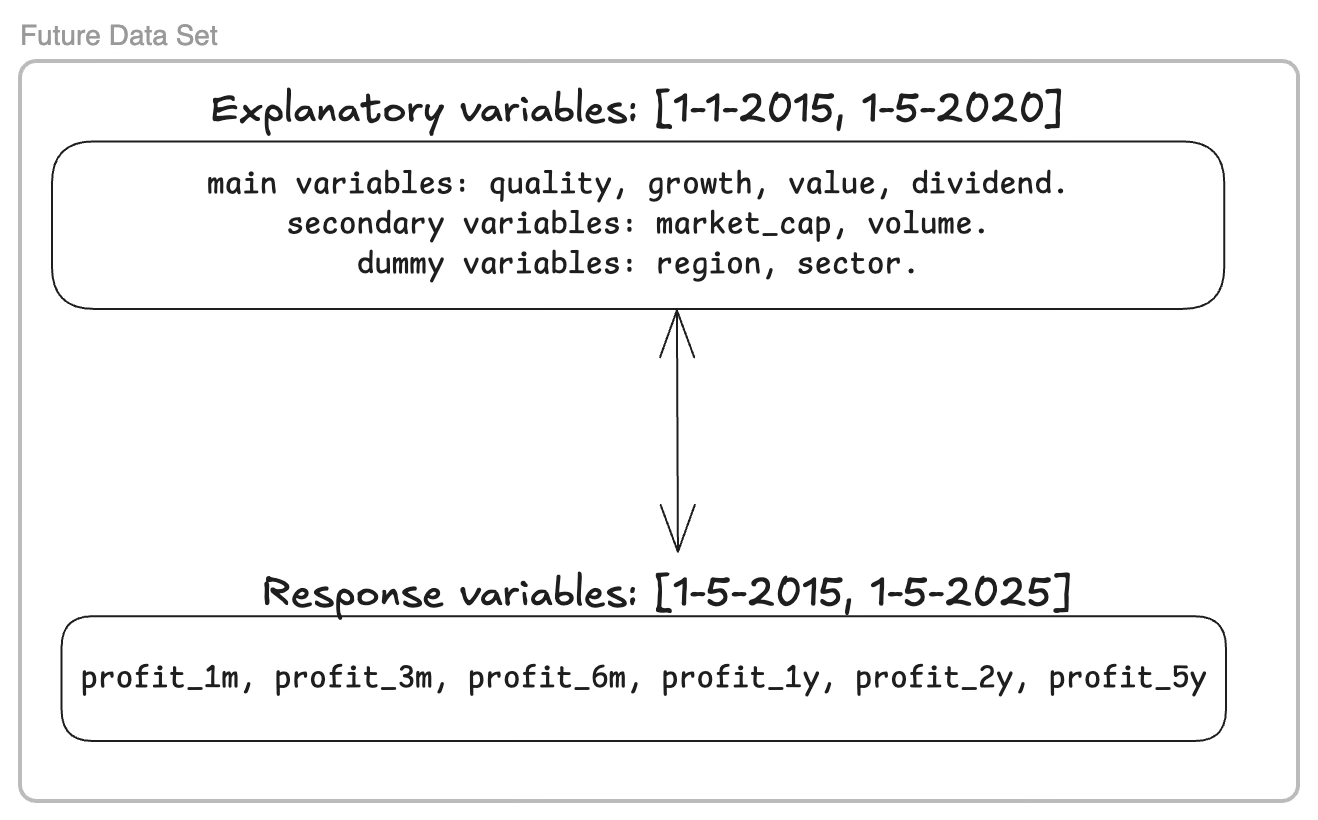
\includegraphics[width=\textwidth]{images/tweenvest/Future Dataset variables relations.png}
        \caption{Future Dataset}
        \label{fig:future_dataset}
    \end{minipage}
\end{figure}

\noindent For the past dataset, we calculated the scores for the range 2020-2025 and then related them to the profits obtained until the specified date. For example, the date 1-1-2021 would be linked to the 2 years' profitability obtained until that date: 
\begin{equation}
    Profit_{1\text{-}1\text{-}2021}(\%) = \frac{P_{1\text{-}1\text{-}2021} - P_{1\text{-}1\text{-}2019} + D_{\text{acc}}}{P_{1\text{-}1\text{-}2019}}
\end{equation}

\noindent Which interprets to \textbf{how earlier profits have influenced on the explanatory variables}. This will give us valuable information in the descriptive analysis.

\vspace{0.5cm}
\noindent For the model fitting, \textbf{we want to know if the current scores are good predictors of future profits}. So we calculated the scores for the range 2015-2020 and related them to the profits obtained from that date to the future. For example, the date 1-1-2021 would be linked to the 2 years' profitability that will be obtained in the future: 

\begin{equation}
    Profit_{1\text{-}1\text{-}2021}(\%) = \frac{P_{1\text{-}1\text{-}2023} - P_{1\text{-}1\text{-}2021} + D_{\text{acc}}}{P_{1\text{-}1\text{-}2021}}
\end{equation}

\noindent As this approach is what we actually want to use for the predictive models, we will be using the future dataset structure for most of the analysis.

\subsection{Preprocessing}
Even with all of the protocols created to have the most reliable and filled datasets, we still had to follow the methodologies explained in the previous chapter to analyze the data and see if there were any problems not solved.

\subsubsection{Cleaning the Data}
To begin, when looking at the data structure we saw that \textbf{about 50\% of growth scores were empty}. This turned on many alerts from problems with the scores calculation algorithm, because compared to the rest of the variables there was a significant difference, since the \textbf{normal absence was only around 8\%}.
\begin{table}[H]
    \centering
    \caption{Missing values (\% ) per column for Small Data Future.}
    \begin{tabular}{|c|c|c|c|c|c|c|c|c|}
        \hline
        \textbf{quality} & \textbf{growth} & \textbf{value} & \textbf{profit\_1m} & \textbf{profit\_3m} & \textbf{profit\_6m} & \textbf{profit\_1y} & \textbf{profit\_2y} & \textbf{profit\_5y} \\
        \hline
        13.4 & 54.0 & 7.4 & 2.6 & 3.1 & 3.2 & 3.2 & 3.3 & 6.0 \\
        \hline
    \end{tabular}
    \label{tab:missing_values_small_data_future}
\end{table}


\noindent   But after digging into the data we saw that it was due to the fact that many companies stopped sending reports or selling but kept existing, so we decided to deleted them from our dataset because they were not behaving as a "normal company", and this could create a bias in the models. Additionally, as noted earlier, we replaced all empty values in the dividend scores with 0, since Tweenvest's algorithm omits a score when a company does not pay dividends. That's why we do not see any missing values in the dividend scores.

\subsection{Outlier Detection}

% TODO: Cohesionate this with last chapter.

In this section we will present the performance of the different outlier detection methods. But the main analysis of the final datasets will be done in the results chapter.

\subsubsection{Inter Quartile Range}

This method is useful for big datasets that need to be filtered quickly and where the meaning of the outliers is not multivariate. But as it will be explained in the results chapter, we saw correlations between the different profits, so we needed to use multivariate outlier detection methods, otherwise we could be creating a bias in the data for the model fitting.

\subsubsection{Isolation Forest}

We started of using this technique due to its speed and accuracy for non-linear multivariate clusters.

\begin{figure}[H]
    \centering
    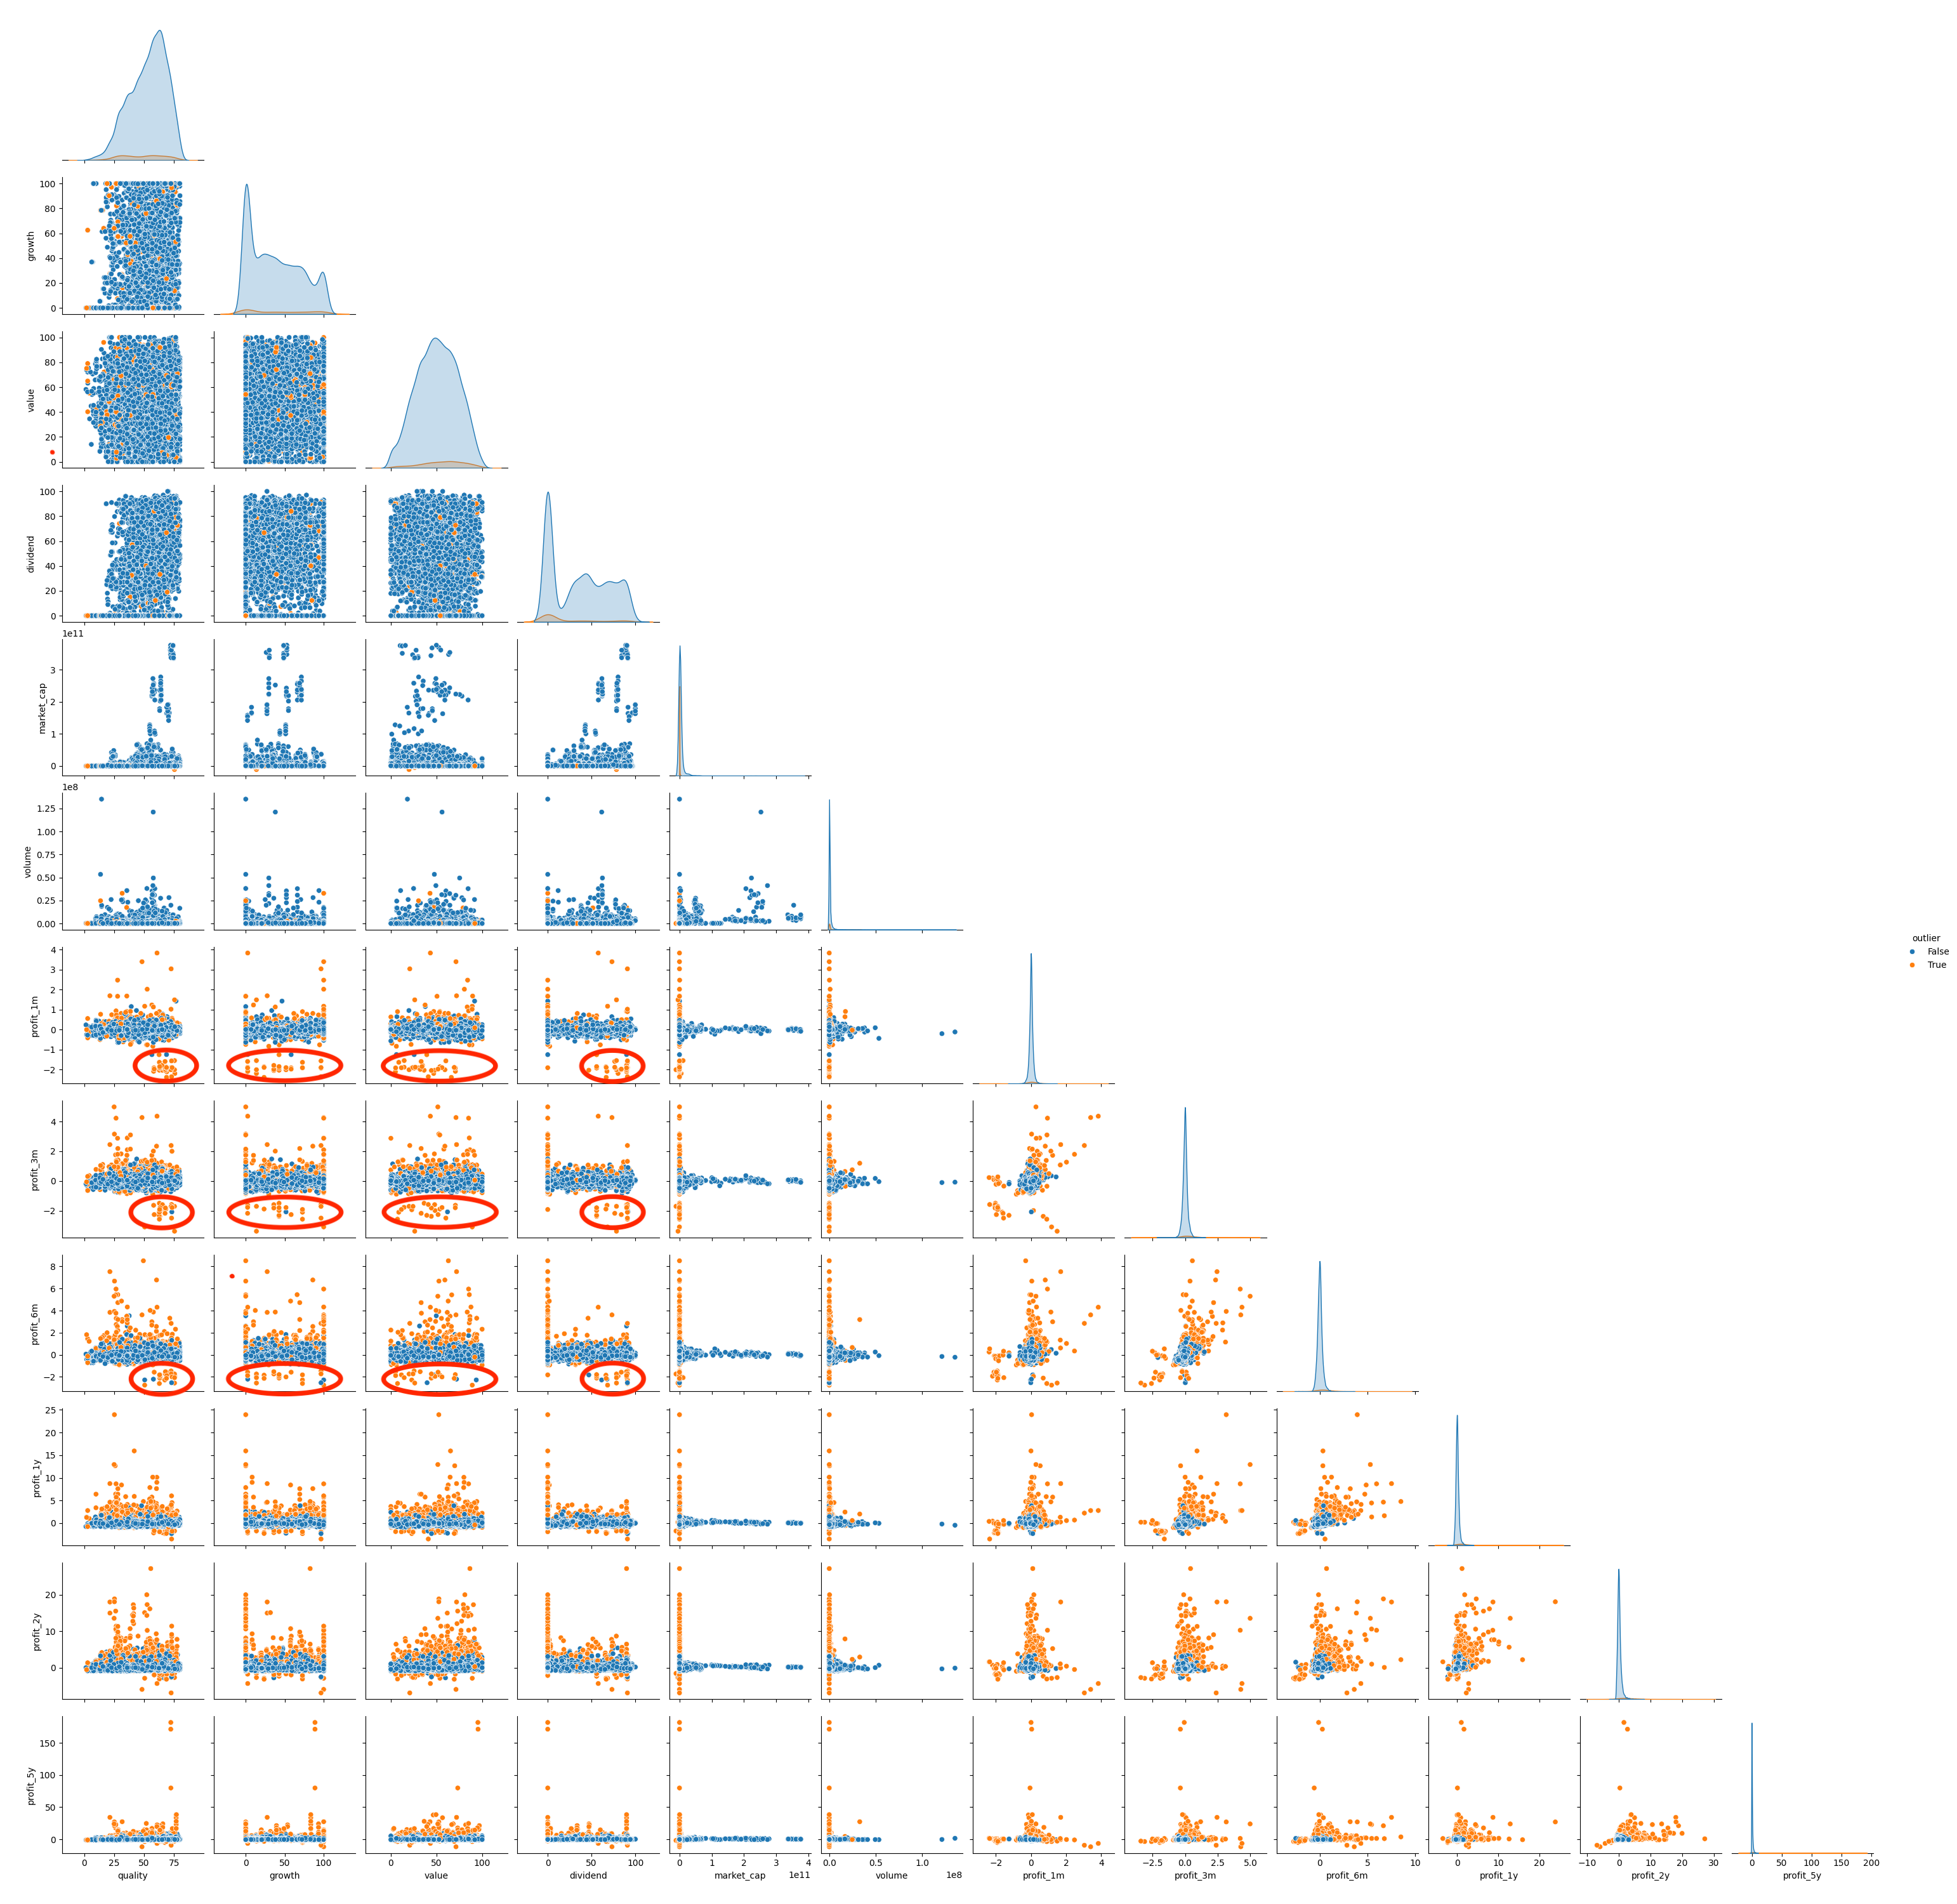
\includegraphics[width=1\textwidth]{images/code/outliers/Small Data future - IF.png}
    \caption{Small Data Future - \acrshort{if} (4\%) \acrshort{pairplot}}
    \label{fig:small_data_future_if}
\end{figure}

\noindent This \acrshort{pairplot} shows how the \acrshort{if} method is detecting outliers in the profits data. In this case it is detecting as outliers much of the data that seems to form a structure in the profits. Also, it is deleting some interesting clusters when comparing the profits with the scores, and here we might lose some important information-- this is highlighted with the red circles.

\newpage

\subsubsection{Single Vector Machine}

When using the \acrshort{svm} we saw a similar detection compared to the \acrshort{if} method, which is very interesting since their approach is completely different.


\begin{figure}[H]
    \centering
    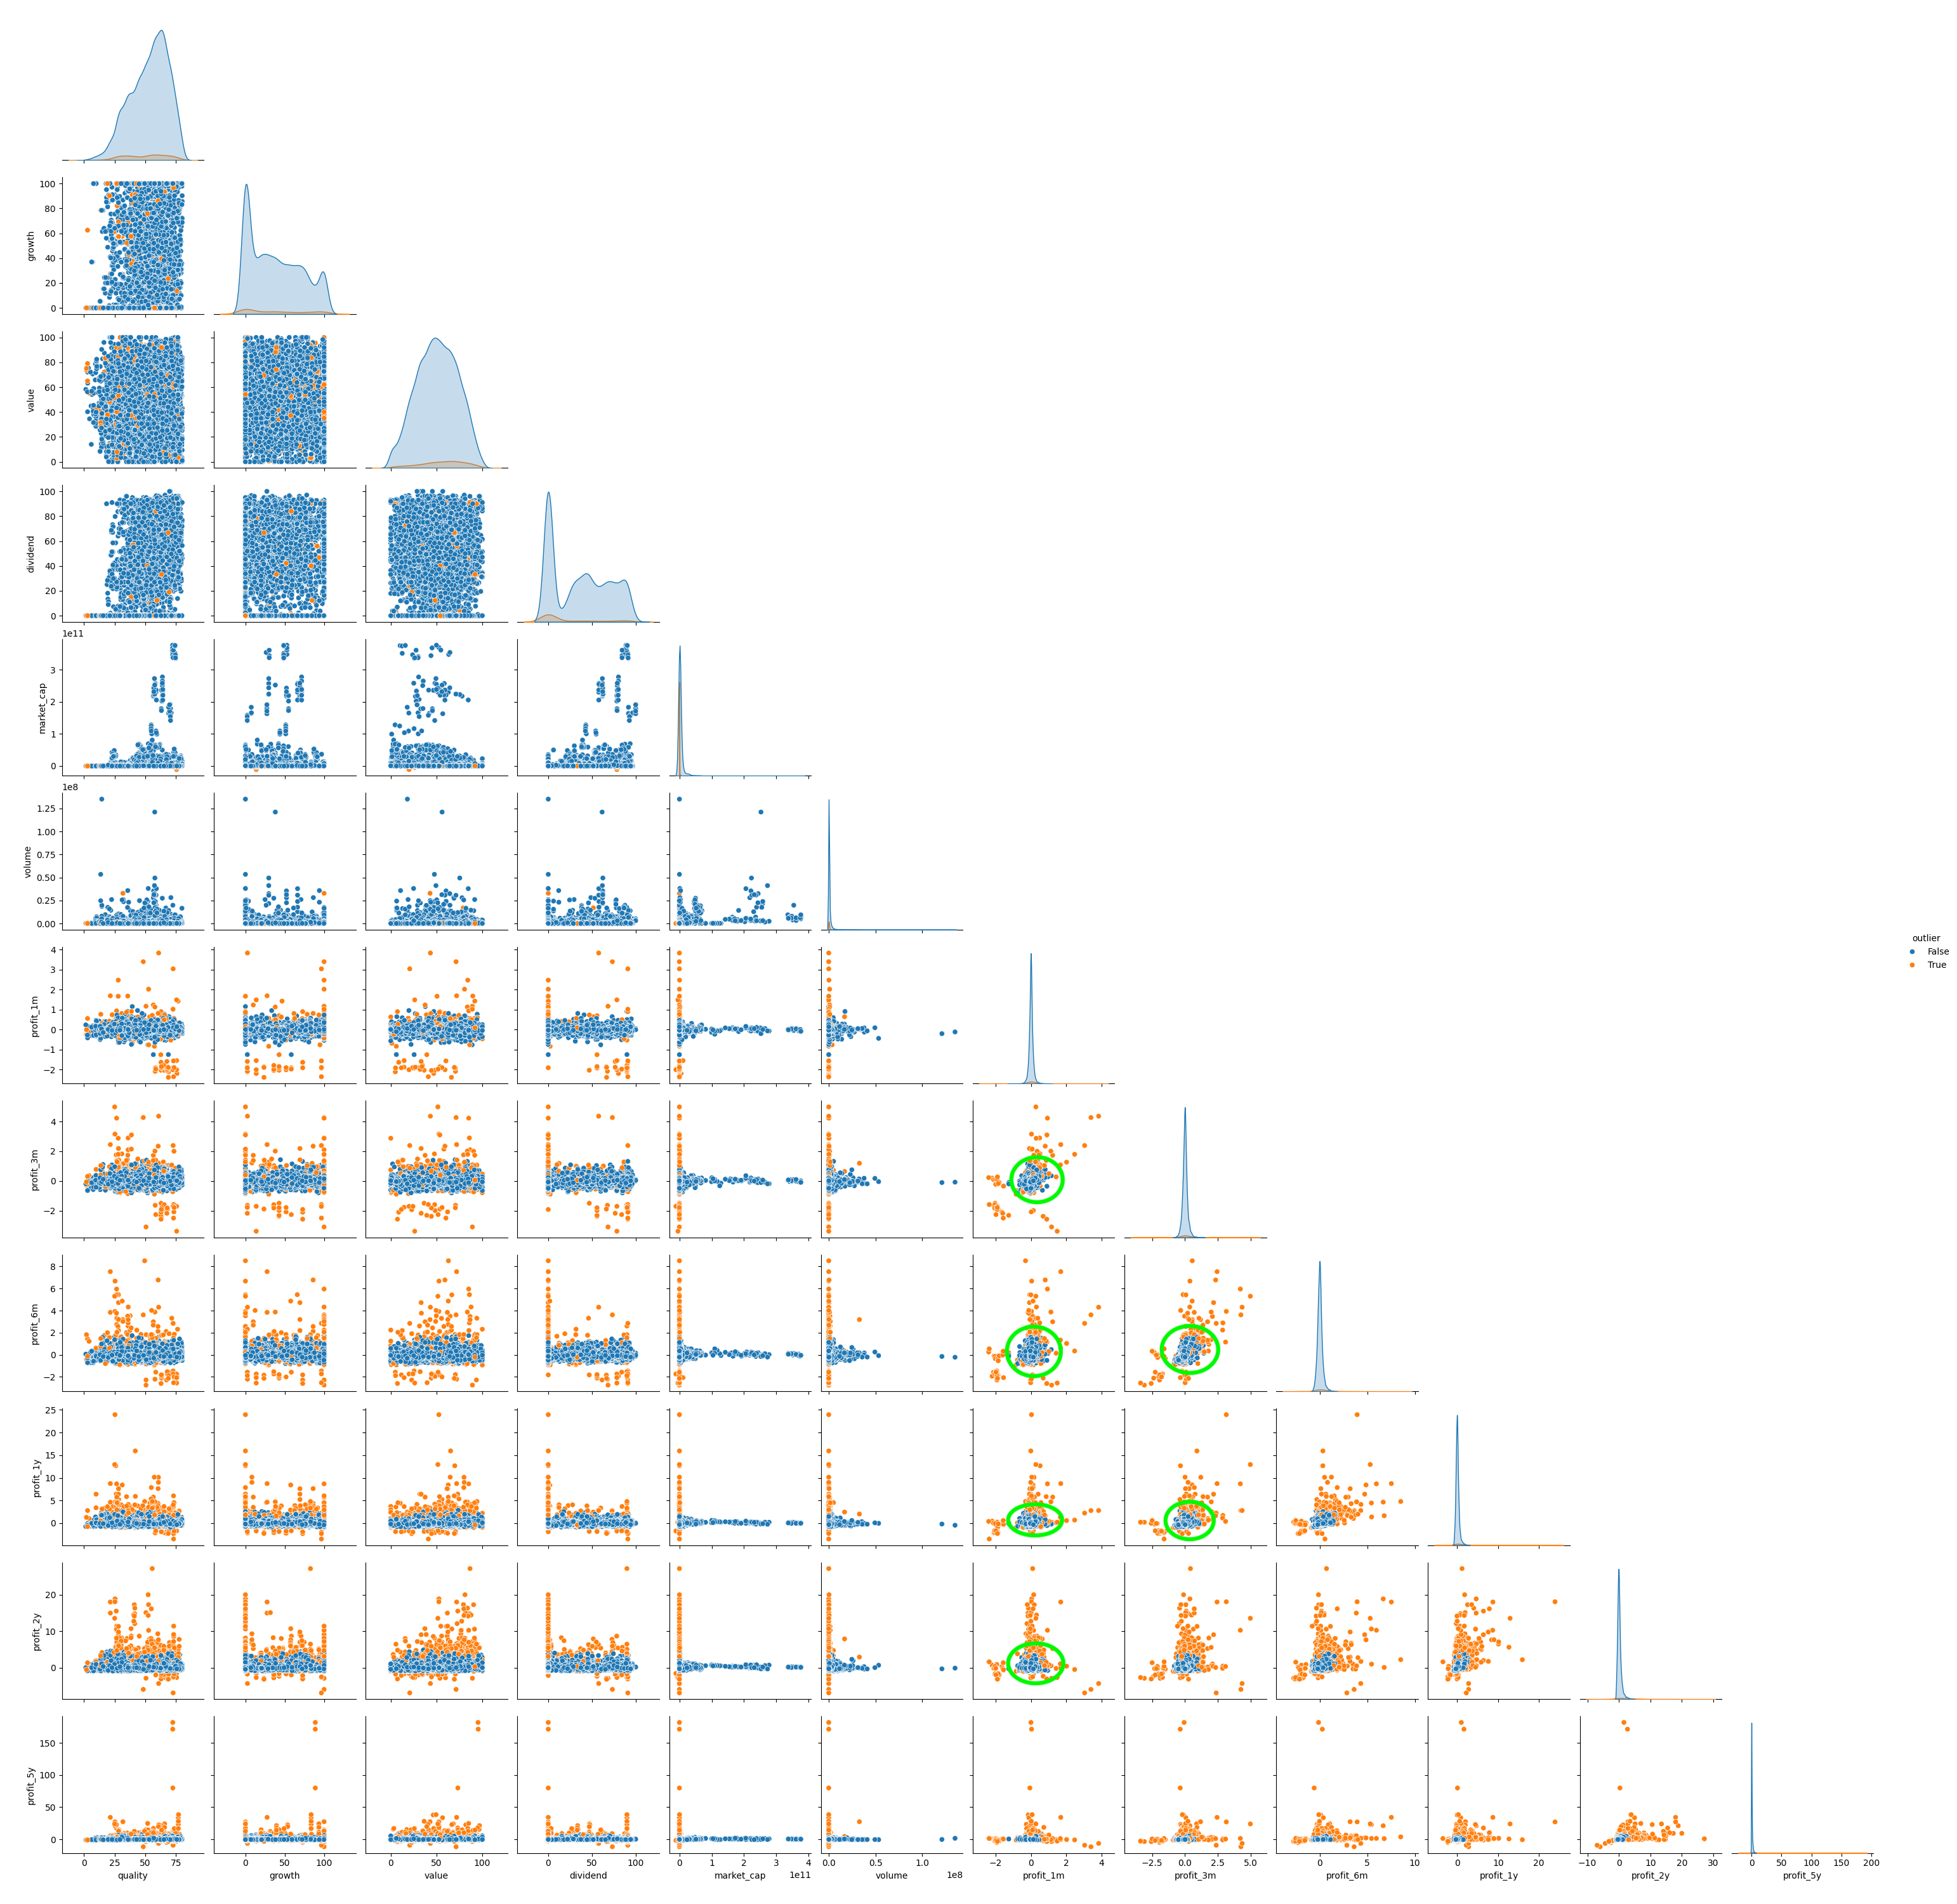
\includegraphics[width=1\textwidth]{images/code/outliers/Small Data future - SVM.png}
    \caption{Small Data Future - \acrshort{svm} (4\%) \acrshort{pairplot}}
    \label{fig:small_data_future_svm}
\end{figure}

\noindent But in this case we also see a slight improvement with recuperating the structures in some of the profits--  this is circled with the green color.

\newpage
\subsubsection{Local Outlier Factor}

\noindent Surprisingly, with the \acrshort{lof} method we see a good improvement for both the profits and the scores clusters-- which is highlighted with the green circles.

\begin{figure}[H]
    \centering
    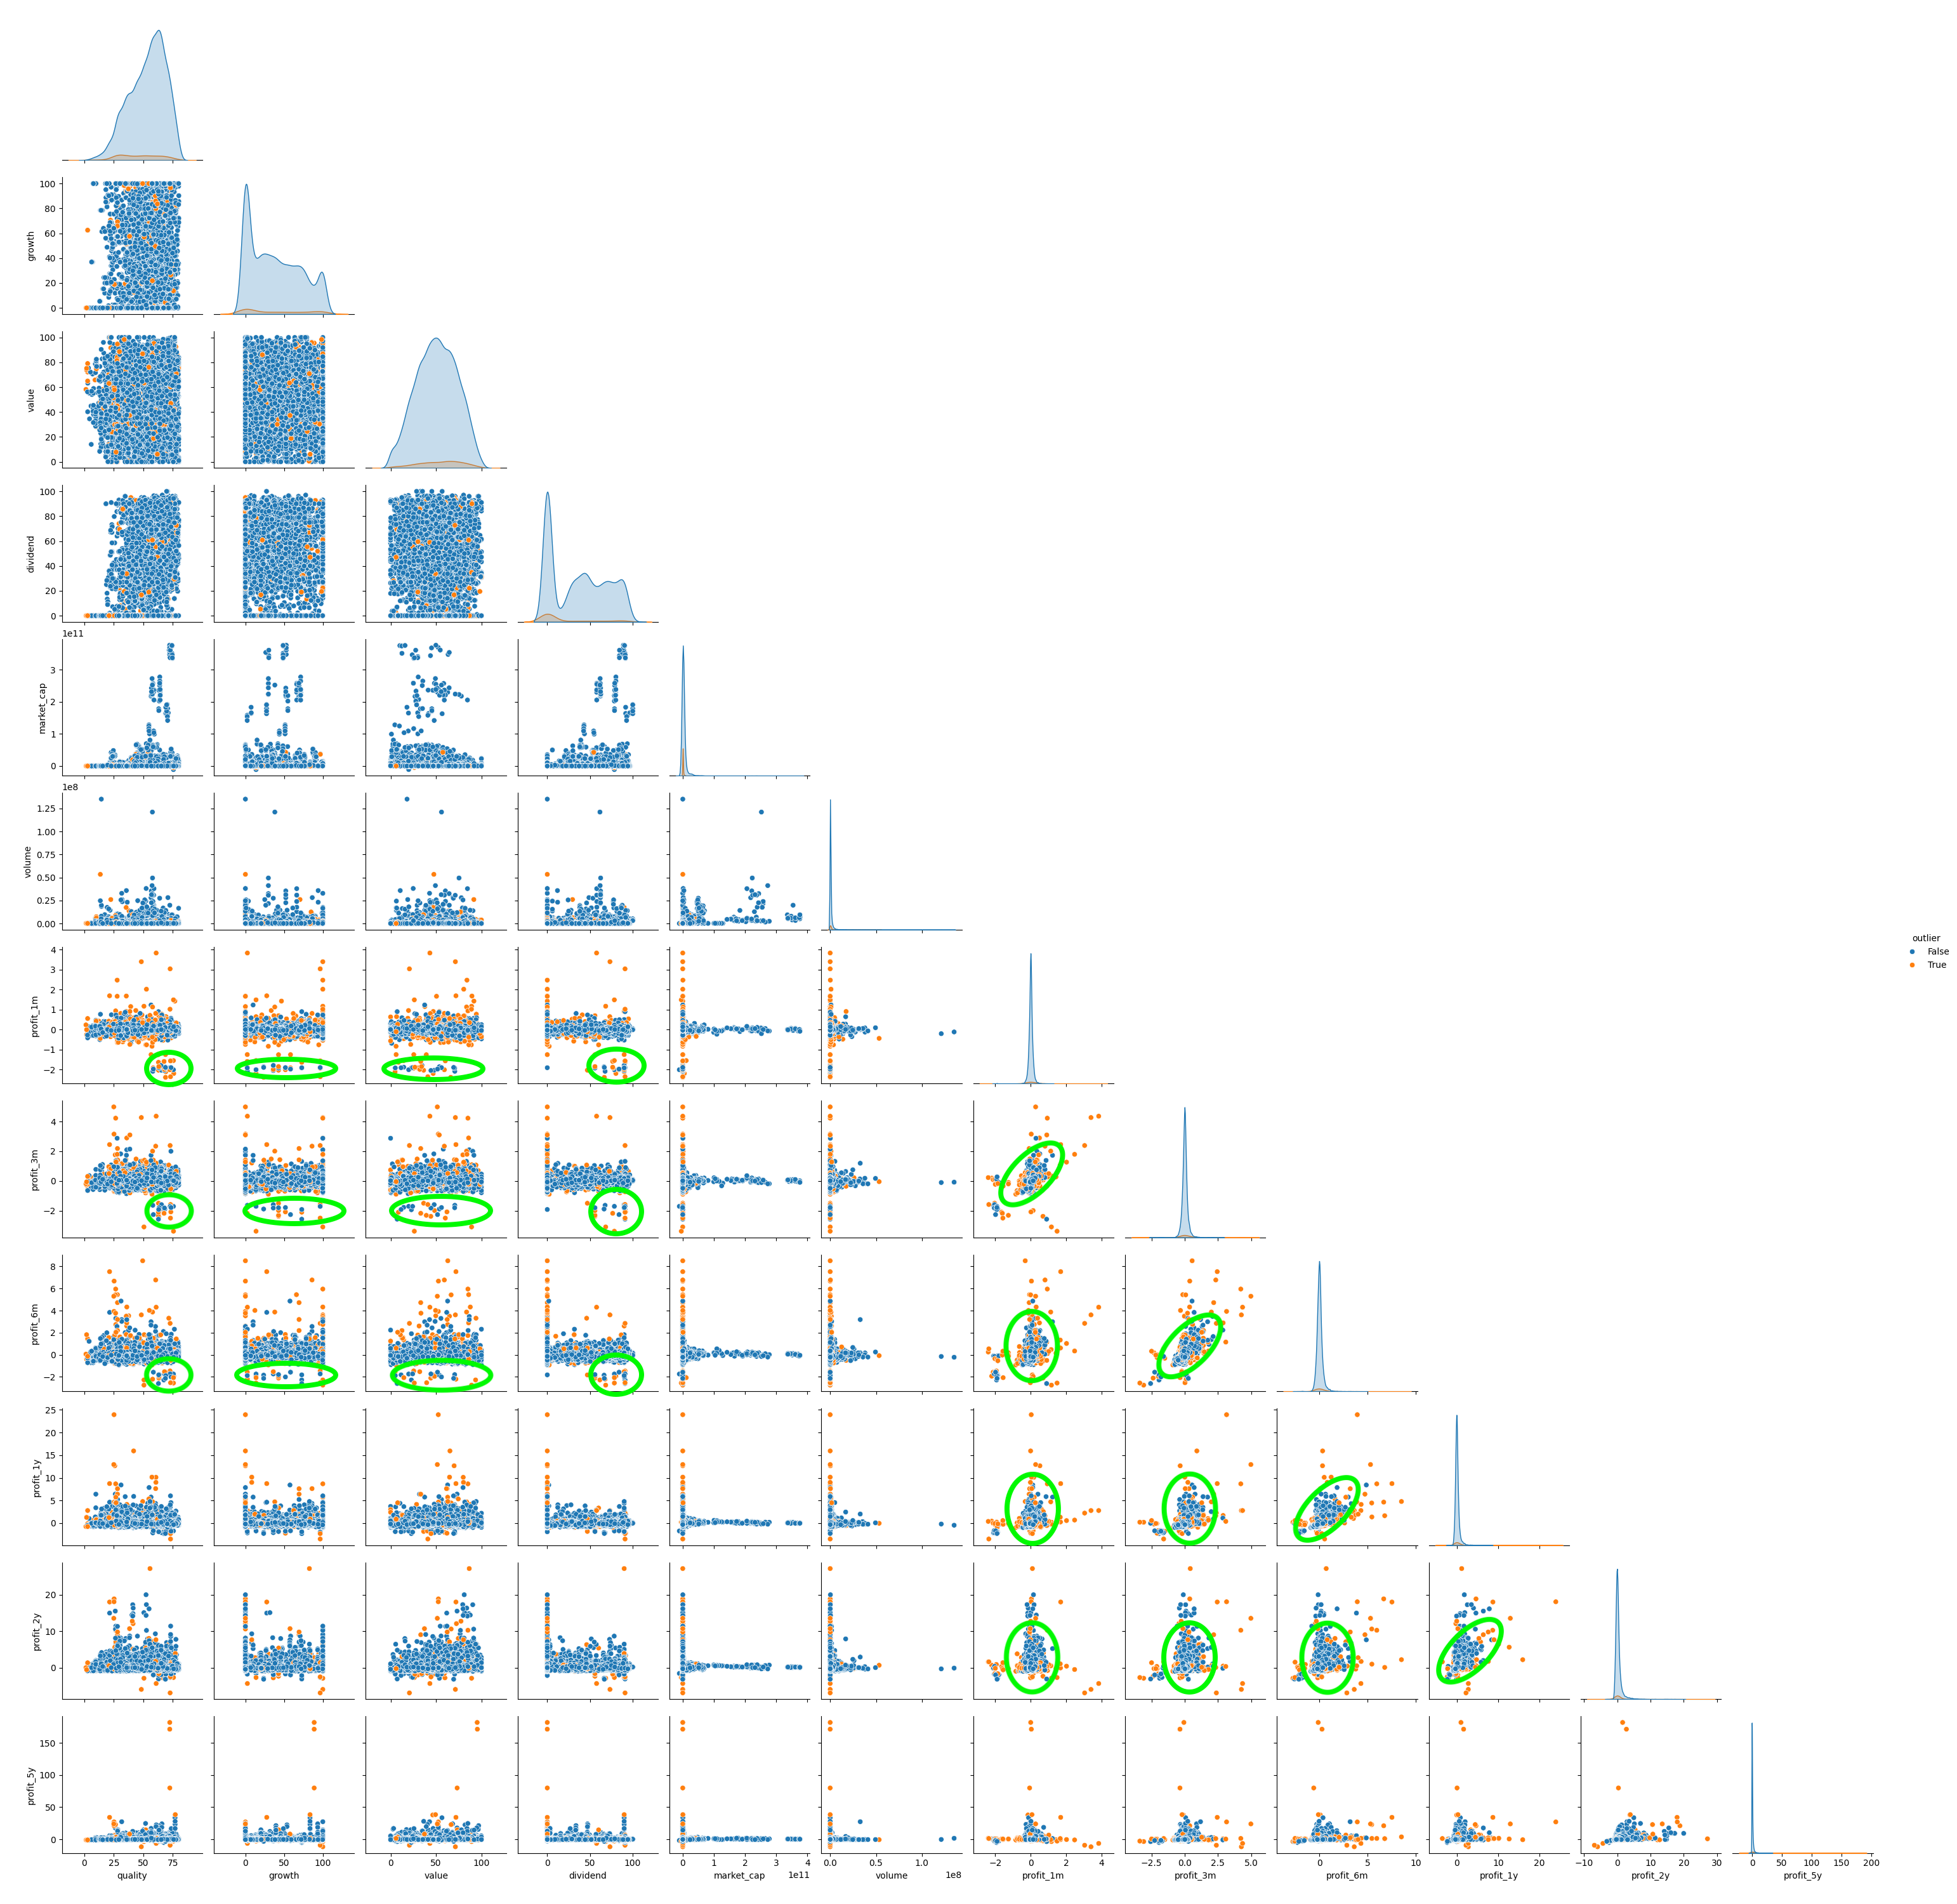
\includegraphics[width=1\textwidth]{images/code/outliers/Small Data future - LOF.png}
    \caption{Small Data Future - \acrshort{lof} (4\%) \acrshort{pairplot}}
    \label{fig:small_data_future_lof}
\end{figure}

\noindent We knew we were going in the right direction, but with this method we were missing some outliers that were detected before in the score-profits clusters.

\newpage
\subsubsection{Multi-Criteria Outlier Detection}

That's when we realized that if each method was good at detecting some outliers but bad at others, so it made a lot of sense to use them together. Following this approach and after multiple tests, we found that the bests results came when increasing the overall tolerance and then selecting the intersection of outliers between them, so with a 20\% tolerance we only excluded around 8\% of the data.

\begin{figure}[H]
    \centering
    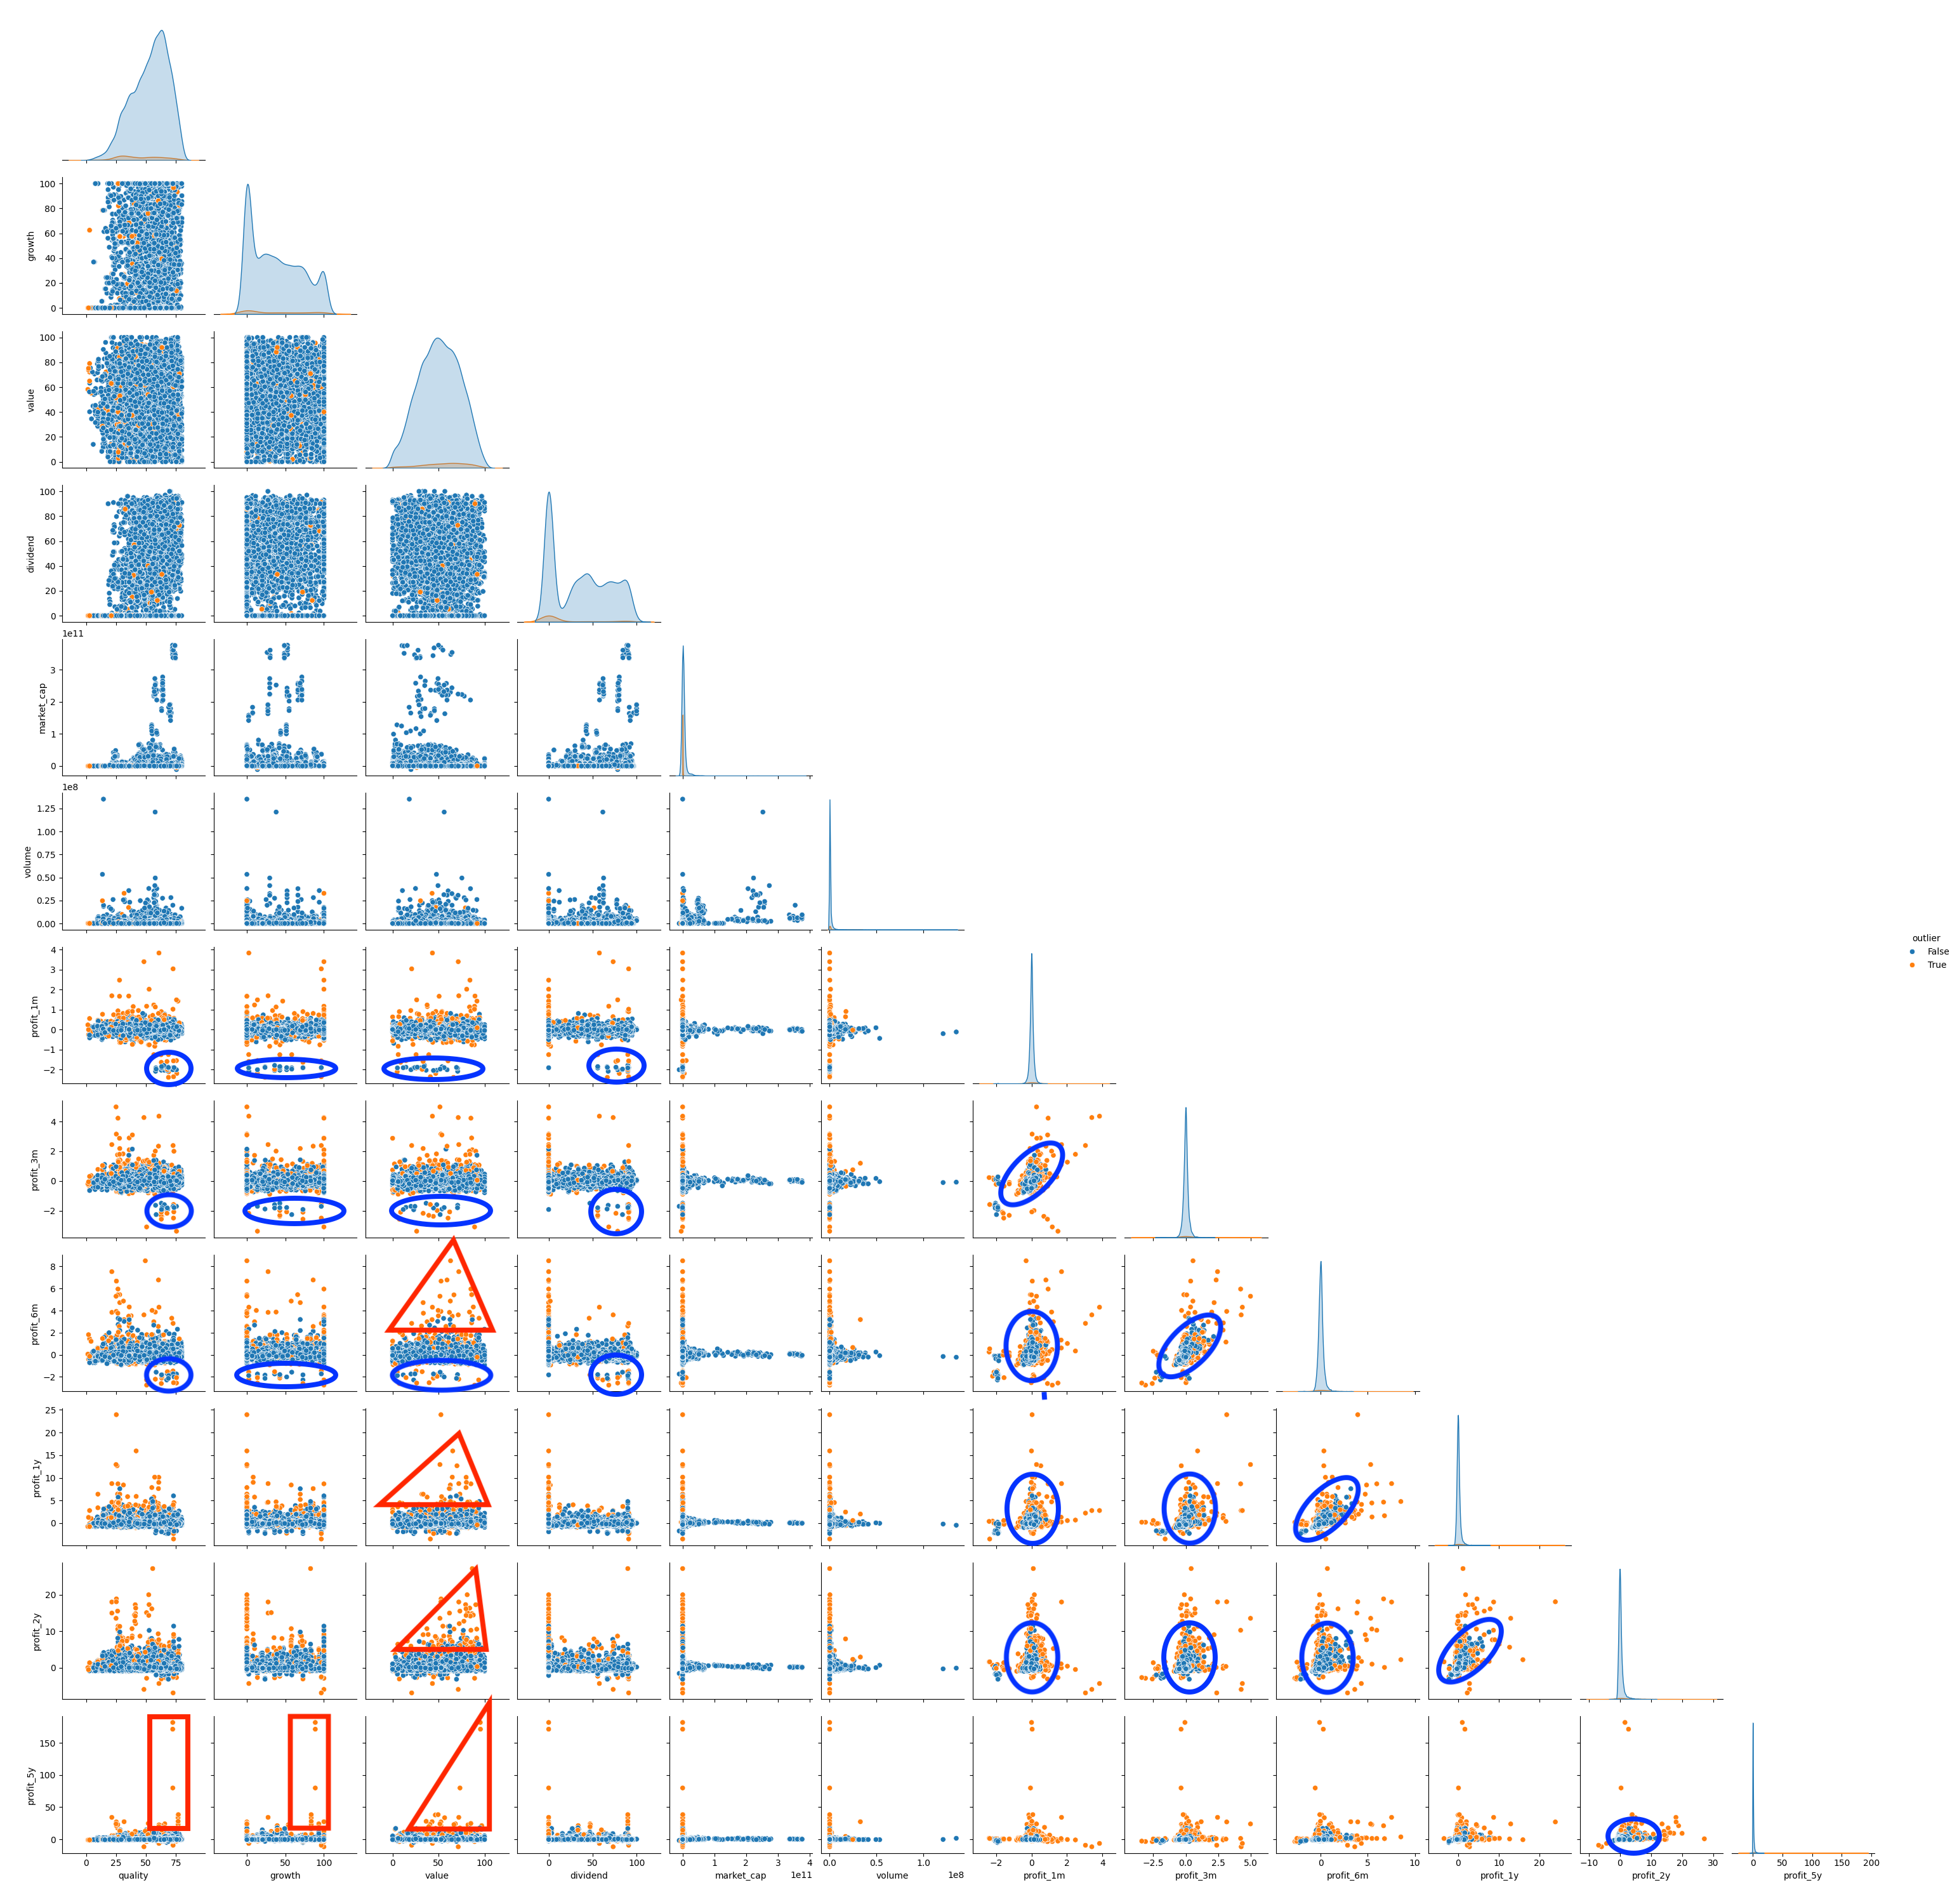
\includegraphics[width=1\textwidth]{images/code/outliers/Small Data future - Multi.png}
    \caption{Small Data Future - \acrshort{multi} (8\%) \acrshort{pairplot}}
    \label{fig:small_data_future_multi}
\end{figure}

\noindent As shown in the \acrshort{pairplot}, this method is able to maintain most of the structures of the profits and also keep the small clusters for the scores, which is highlighted with the blue circles. But of course, it is not perfect and could be missing important information for extreme cases --highlighted with the red shapes. 


\subsubsection{Islands of Outliers}

\noindent After the previous results we started working with the models, but we quickly noticed that those clusters that were not being deleted, on purpose, were affecting the results. So we decided to take a big look at the data again to see what was happening:

\begin{figure}[H]
    \centering
    \begin{minipage}{0.32\textwidth}
        \centering
        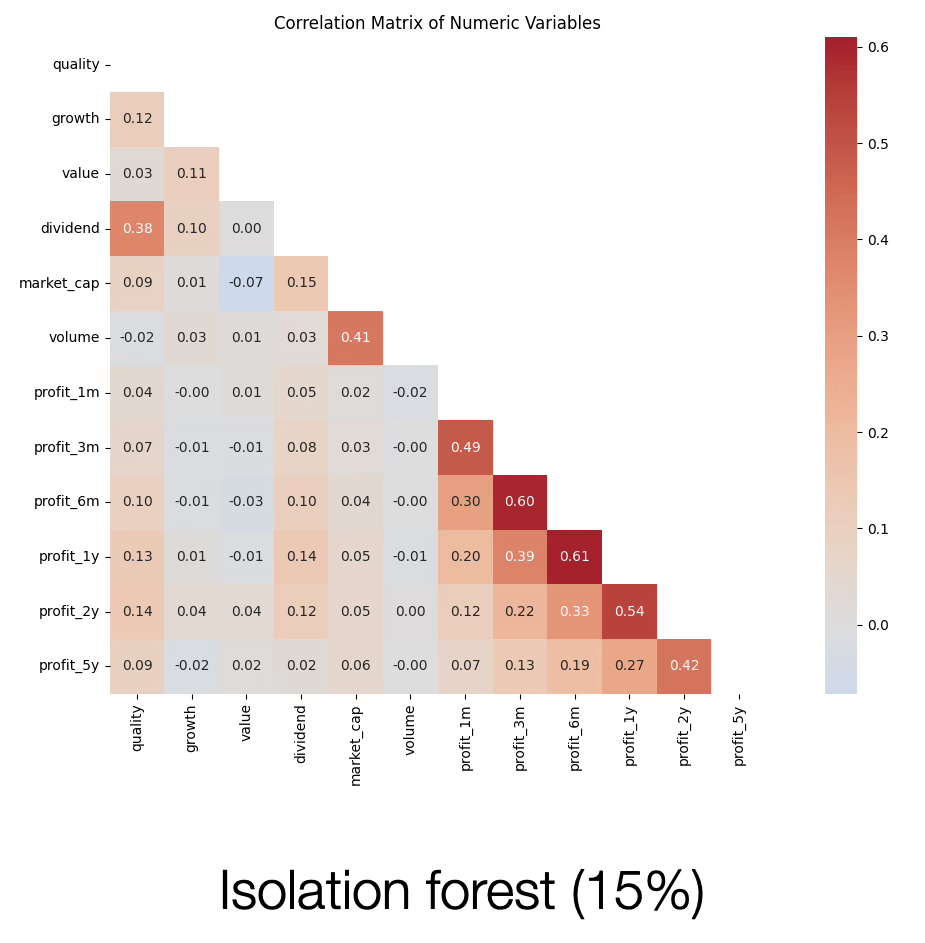
\includegraphics[width=\textwidth]{images/code/outliers/IF 15.png}
    \end{minipage}
    \hfill
    \begin{minipage}{0.32\textwidth}
        \centering
        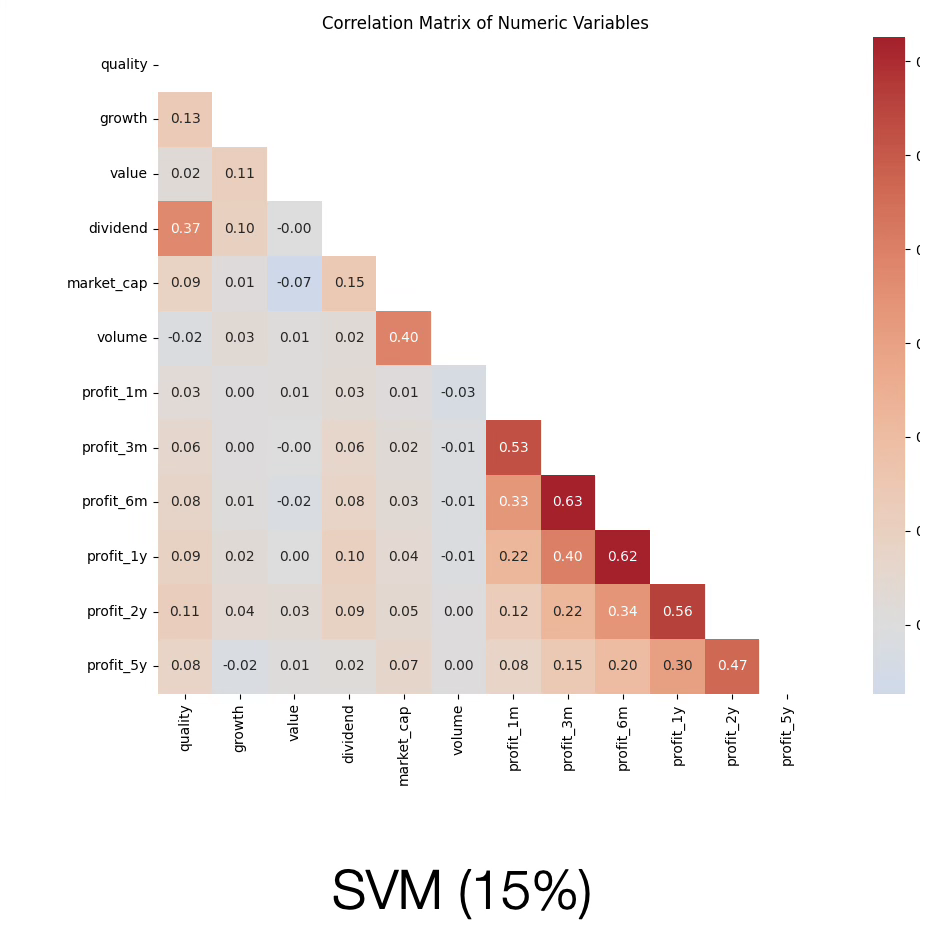
\includegraphics[width=\textwidth]{images/code/outliers/SVM 15.png}
    \end{minipage}
    \hfill
    \begin{minipage}{0.32\textwidth}
        \centering
        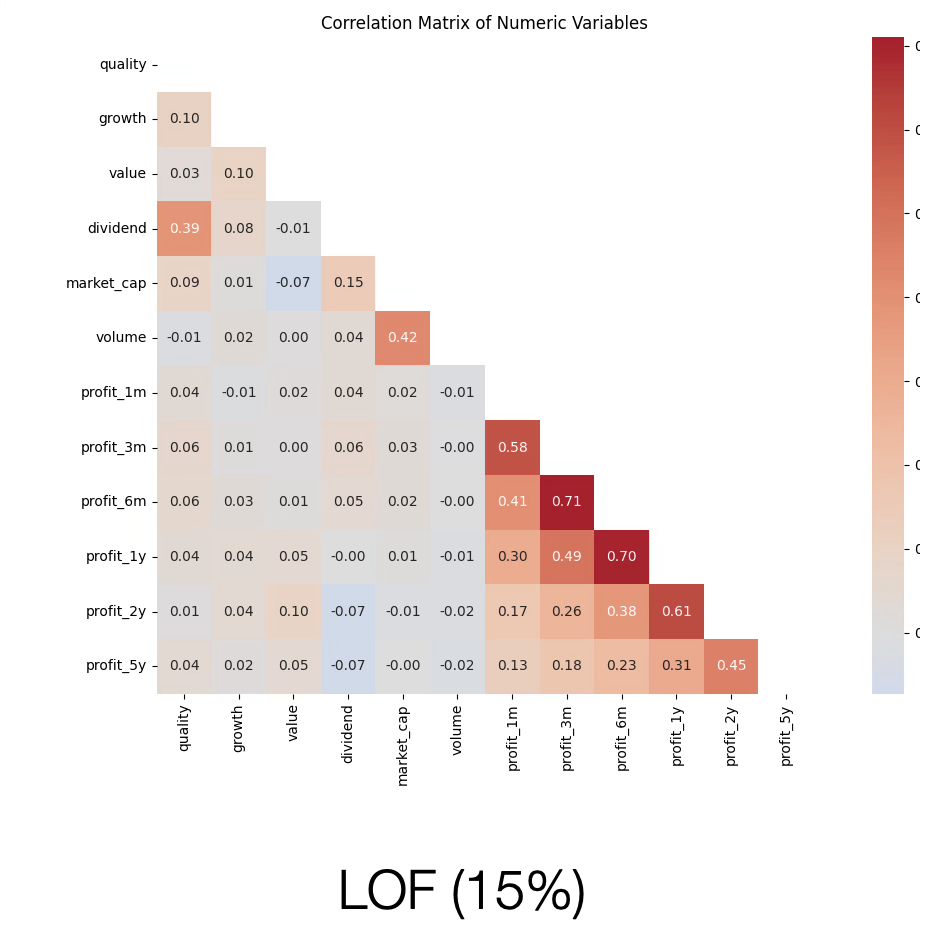
\includegraphics[width=\textwidth]{images/code/outliers/LOF 15.png}
    \end{minipage}
    \caption{Correlations between variables for different outlier detection methods}
    \label{fig:island_cases_examples}
\end{figure}

\noindent As we can see, the \acrshort{if} and \acrshort{svm} methods are showing some correlations between the profits and the scores, but the \acrshort{lof} is not showing any correlations, even negative ones. And that is what made us think about the clusters of anomalies that were not being deleted by the \acrshort{lof} method, so we built the \acrshort{islandcase}, mentioned in the previous section.





% TODO: Move this to the future work section:

% \vspace{0.5cm}
% \noindent For future developments of these type of techniques, we have to mention that understanding the main core ideas of each method we could probably optimize the results by changing the tolerance parameters individually by applying multipliers for each method:
% \begin{enumerate}
%     \item \textbf{\acrshort{svm}} is basically creating geometrical hyper-dimensional frontiers to form a safe hyper-volume of data clusters. So the intuition tells us that this method should probably have a \textbf{higher tolerance} than the rest.
%     \item \textbf{\acrshort{lof}} is looking for clusters of high density, not taking account the distance between the clusters. So this method is very good for detecting extreme phenomena but that could be consistent. Its \textbf{tolerance could be between the other methods}.
%     \item \textbf{\acrshort{if}} is looking for the most isolated points following a random forest approach. It is good for detecting those points that seem to make not much sense, so its \textbf{tolerance should not be as high}.
% \end{enumerate}

% \noindent But this is just a hypothesis, we will have to be studied it in the future with rigorous tests.


\subsection{Summary}

\noindent To summarize how we have treated the data, we ended up with different datasets groups, each with 17 columns for the explained variables, the date and also the company's name and stock ticker (see appendix figure~\ref{fig:number_of_columns}).

\subsubsection{Simple Datasets}
\noindent For the first part of the analysis that consisted of the descriptive analysis, we started by using the Big Datasets, that contain all of the Tweenvest's data for the past 10 years. This way we could see the real distributions and correlations, as we will explain in the next chapter. Also we created the 2 subsets of Small Data with only 1,500 stocks for quicker calculations, making sure that the sectors were balanced, and using a \textbf{4\% removal rate} for the \acrshort{multi} method.

\begin{table}[H]
    \centering
    \caption{Simple Datasets Total Rows}
    \begin{tabular}{|l|l|l|l|}
        \hline  
        \textbf{Dataset} & \textbf{Raw} & \textbf{Cleaned} & \textbf{No Outliers} \\
        \hline
        \textbf{Big Data Past$^\dagger$} & 16,119,852 & 9,991,895 & 9,492,300 \\
        \hline
        \textbf{Big Data Future$^\dagger$} & 31,933,137 & 14,518,624 & 13,792,692 \\
        \hline 
        \textbf{Small Data Past} & 83,243 & 48,338 & 46,415 \\
        \hline
        \textbf{Small Data Future} & 65,166 & 26,214 & 25,220 \\
        \hline
        \end{tabular}
    \label{tab:simple_datasets_rows}
\end{table}

\noindent $^\dagger$ In the \textit{Big Data Past} and \textit{Big Data Future} datasets, we removed the outliers using the \acrshort{if} method for saving computational time.

\subsubsection{Geographical Datasets}

\noindent For the second part of the analysis, that consists of exploring the regression models, while advancing with it we had to inspect how the geographical regions were affecting the results, so we created one dataset per region applying the same sector balancing. Here  we kept using the \textbf{4\% removal rate} with the \acrshort{multi}.

\begin{table}[H]
    \centering
    \caption{Geographical Datasets Total Rows}
    \begin{tabular}{|l|l|l|l|}
        \hline  
        \textbf{Dataset} & \textbf{Raw} & \textbf{Cleaned} & \textbf{No Outliers} \\
        \hline
        \textbf{Small Data Future USA} & 60,503 & 21,240 & 20,463 \\
        \hline
        \textbf{Small Data Future EU} & 62,725 & 25,217 & 24,245 \\
        \hline        
        \textbf{Small Data Future AS} & 65,772 & 28,085 & 27,156\\
        \hline
        \textbf{Small Data Future LAT} & 48,412 & 20,610 & 19,851 \\
        \hline
        \textbf{Small Data Future AF} & 58,341 & 21,182 & 20,335 \\
        \hline
        \end{tabular}
    \label{tab:geographical_datasets_rows}
\end{table}

\subsubsection{Restrictive Datasets}
\noindent For the third part of the analysis, once we had seen the nature of the data and the simple models results, we realized how much the outliers and countries were affecting the results, thats why we chose the \acrshort{gam} non-linear models. So for improving the consistency we used the \acrshort{islandcase} and the \acrshort{if} method with higher tolerances.

% TODO: Check which datasets were being used here.

\begin{table}[H]
    \centering
    \caption{Restrictive Datasets Total Rows}
    \begin{tabular}{|l|l|l|l|l|}
        \hline  
        \textbf{Dataset} & \textbf{Raw} & \textbf{Cleaned} & \textbf{ \acrshort{islandcase} 15\%} & \textbf{ \acrshort{if} 15\%} \\
        \hline
        \textbf{Small Data Future} & 65,166 & 26,214 & 22,214 & 22,282 \\
        \hline
        \end{tabular}
    \label{tab:restrictive_datasets_rows}
\end{table}

\subsubsection{Validation Dataset}

\noindent In the final stage of our analysis, our goal was to obtain the most realistic results possible, which required retaining as much data as we could. To achieve this, we revisited the Big Data Future dataset and applied the \acrshort{if} method with a \textbf{very high removal rate of 35\%}. Additionally, we balanced the data by regions and sectors. These steps, however, led to a substantial reduction in the number of rows.

\begin{table}[H]
    \centering
    \caption{Validation Datasets Summary}
    \begin{tabular}{|l|l|l|l|l|}
        \hline  
        \textbf{Dataset} & \textbf{Cleaned} & \textbf{ \acrshort{if} 35\%} & \textbf{{Balanced}} \\
        \hline
        \textbf{Big Data Future} & 14,518,624 & 9,437,105 & 110,203 \\
        \hline
        \end{tabular}
    \label{tab:validation_datasets_summary}
\end{table}

\noindent These restrictions resulted on a surprisingly higher simple correlations, showing that we were going in the right path.

\subsubsection{Conclusion}

\noindent Finally, we have to clarify that outliers are anomalies in the \textit{normal} behavior of the data, so even thought we are excluding them for obtaining a general set of models, we could be missing valuable information such as the possible structures shown with the red structures in the figure~\ref{fig:small_data_future_multi}. That is why we propose for future work a separate analysis for the outliers, to see if really good profits (or bad ones) have any characteristics, such as average high or low scores.

%  TODO: Try to make a small analysis of the outliers.

\chapter{Results}
This chapter presents the outcomes of the analyses and modeling procedures applied to the curated datasets. The results are organized into two main parts. First, a descriptive analysis explores the underlying characteristics of the data, examining distributions, correlations, and clustering patterns to identify preliminary relationships between the scores and company performance. Second, the predictive modeling results evaluate the extent to which the scores --and other explanatory variables-- can be used to anticipate future profitability over different investment horizons.

\section{Descriptive Analysis}

Before jumping into the model fitting, it is necessary to understand the data that we are working with. For doing so, we will be looking at the variables distributions, correlations and possible structures.Through this analysis we will be first looking at the big datasets for understanding the data, and then we will be checking if the small subsets behave similarly. Also, because there are a few outliers in the \textit{Big Data} that makes the profits distributions not very clear, we will be using the \acrshort{iqr} method to remove them.

\subsection{Variables Distributions}

\subsubsection{Scores}
 When looking at the scores in the figure~\ref{fig:scores}, we see that there are several scores that saturate. So for a better visualization we created a temporal dataset where the dividend and growth scores saturating at 0 were deleted, this is shown in the figure~\ref{fig:scores_deep}. 

\begin{figure}[H]
    \centering
    \begin{minipage}{0.5\textwidth}
        \centering
        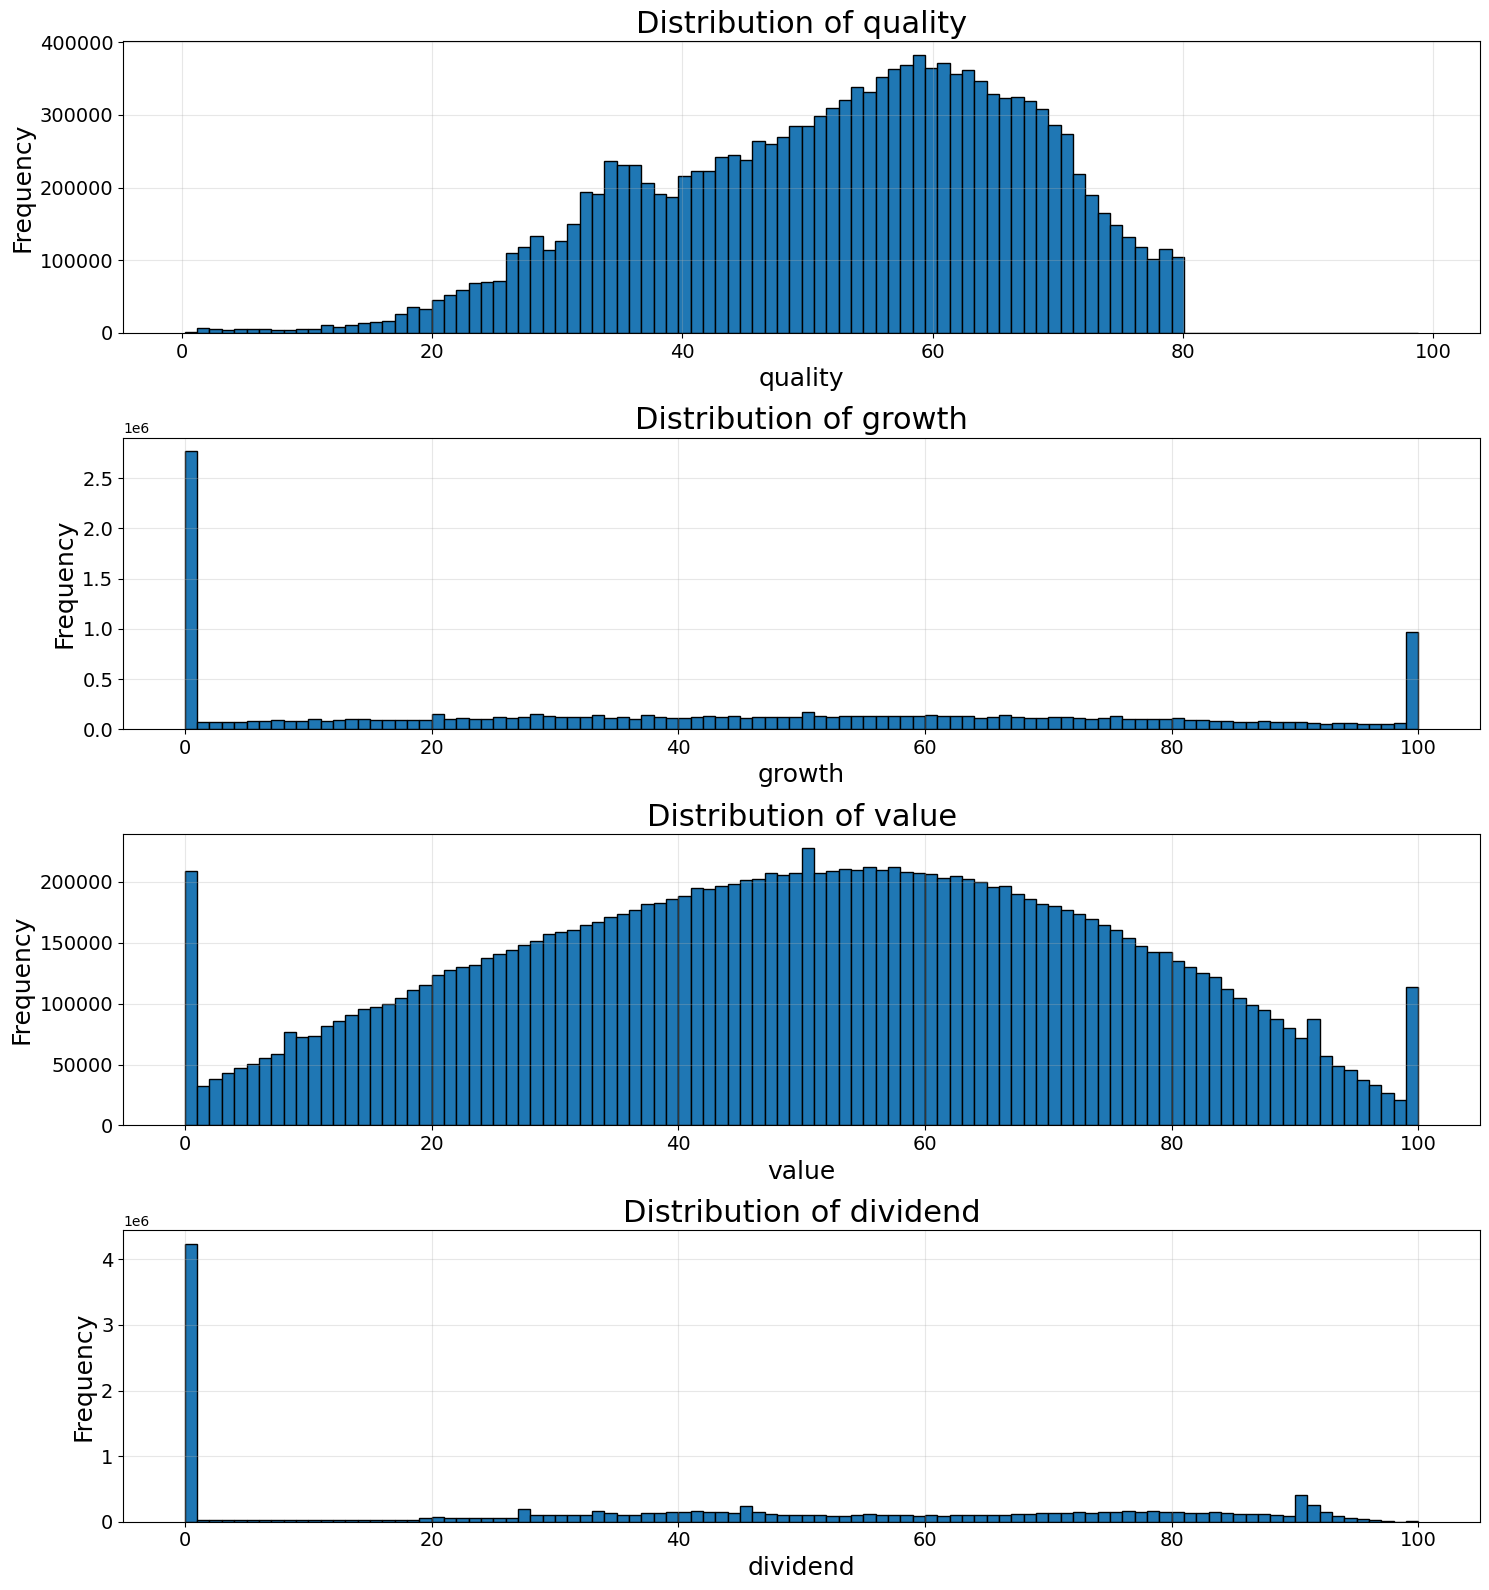
\includegraphics[width=\linewidth]{images/code/descriptive analysis/distributions/Big Data future IQR - Scores.png}
        \caption{Big Data Future (\acrshort{iqr}) - Scores}
        \label{fig:scores}
    \end{minipage}\hfill
    \begin{minipage}{0.5\textwidth}
        \centering
        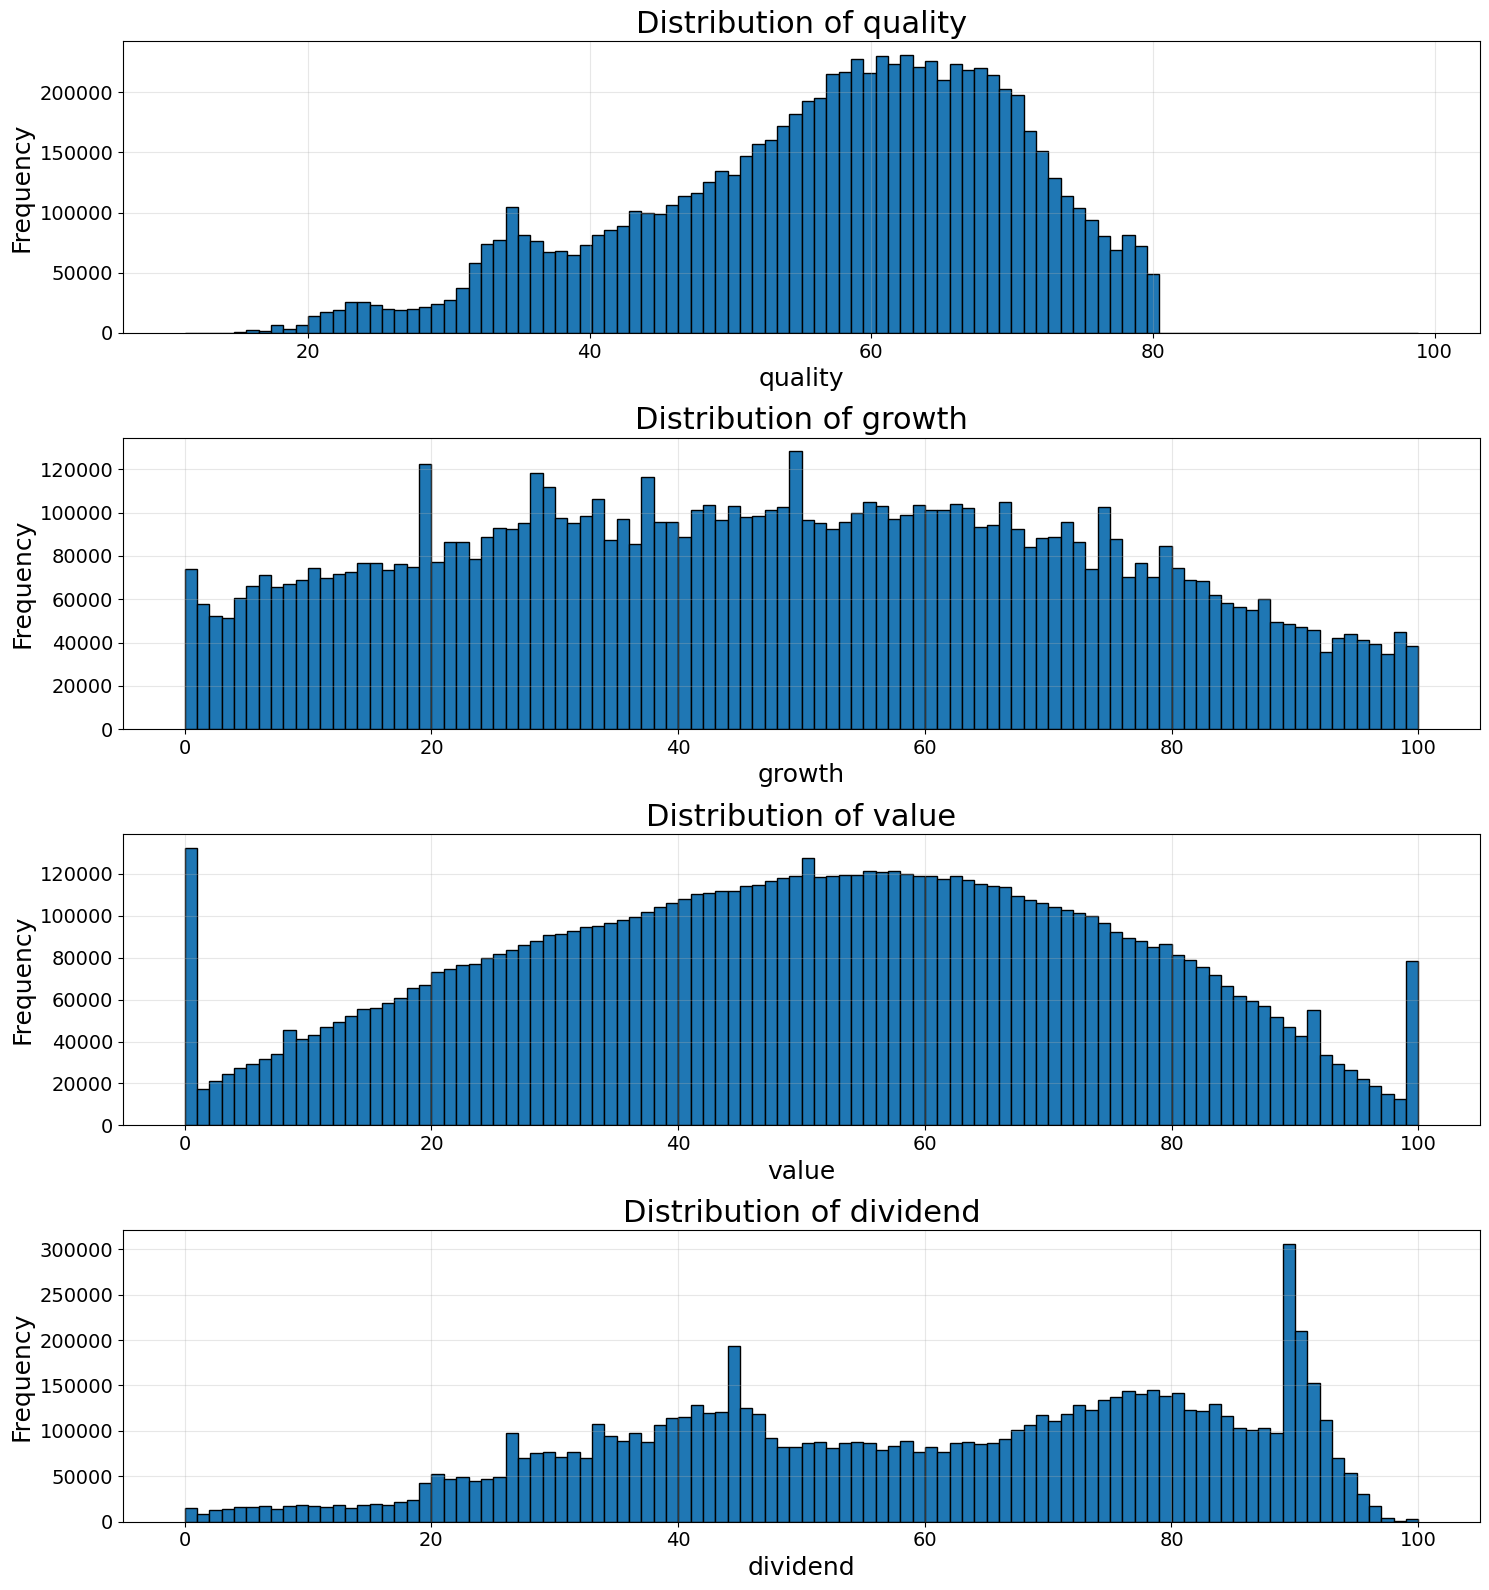
\includegraphics[width=\linewidth]{images/code/descriptive analysis/distributions/Big Data future IQR - Scores Deep.png}
        \caption{Big Data Future (\acrshort{iqr}) - Scores Deep}
        \label{fig:scores_deep}
    \end{minipage}
\end{figure}

\noindent Starting with the \textbf{quality score}, we can see that its distribution shows a \textbf{clear negative skewness}, meaning that there are more companies closer to having a good quality score. This could be due to the fact that we had deleted companies that did not behave as a ``normal company'', so we will later analyze the distributions of the profits to see if this was the case. Also, there is a \textbf{secondary peak around the 30-40 scores}, which could be related to the time-frame of the data.

\begin{figure}[H]
    \centering
    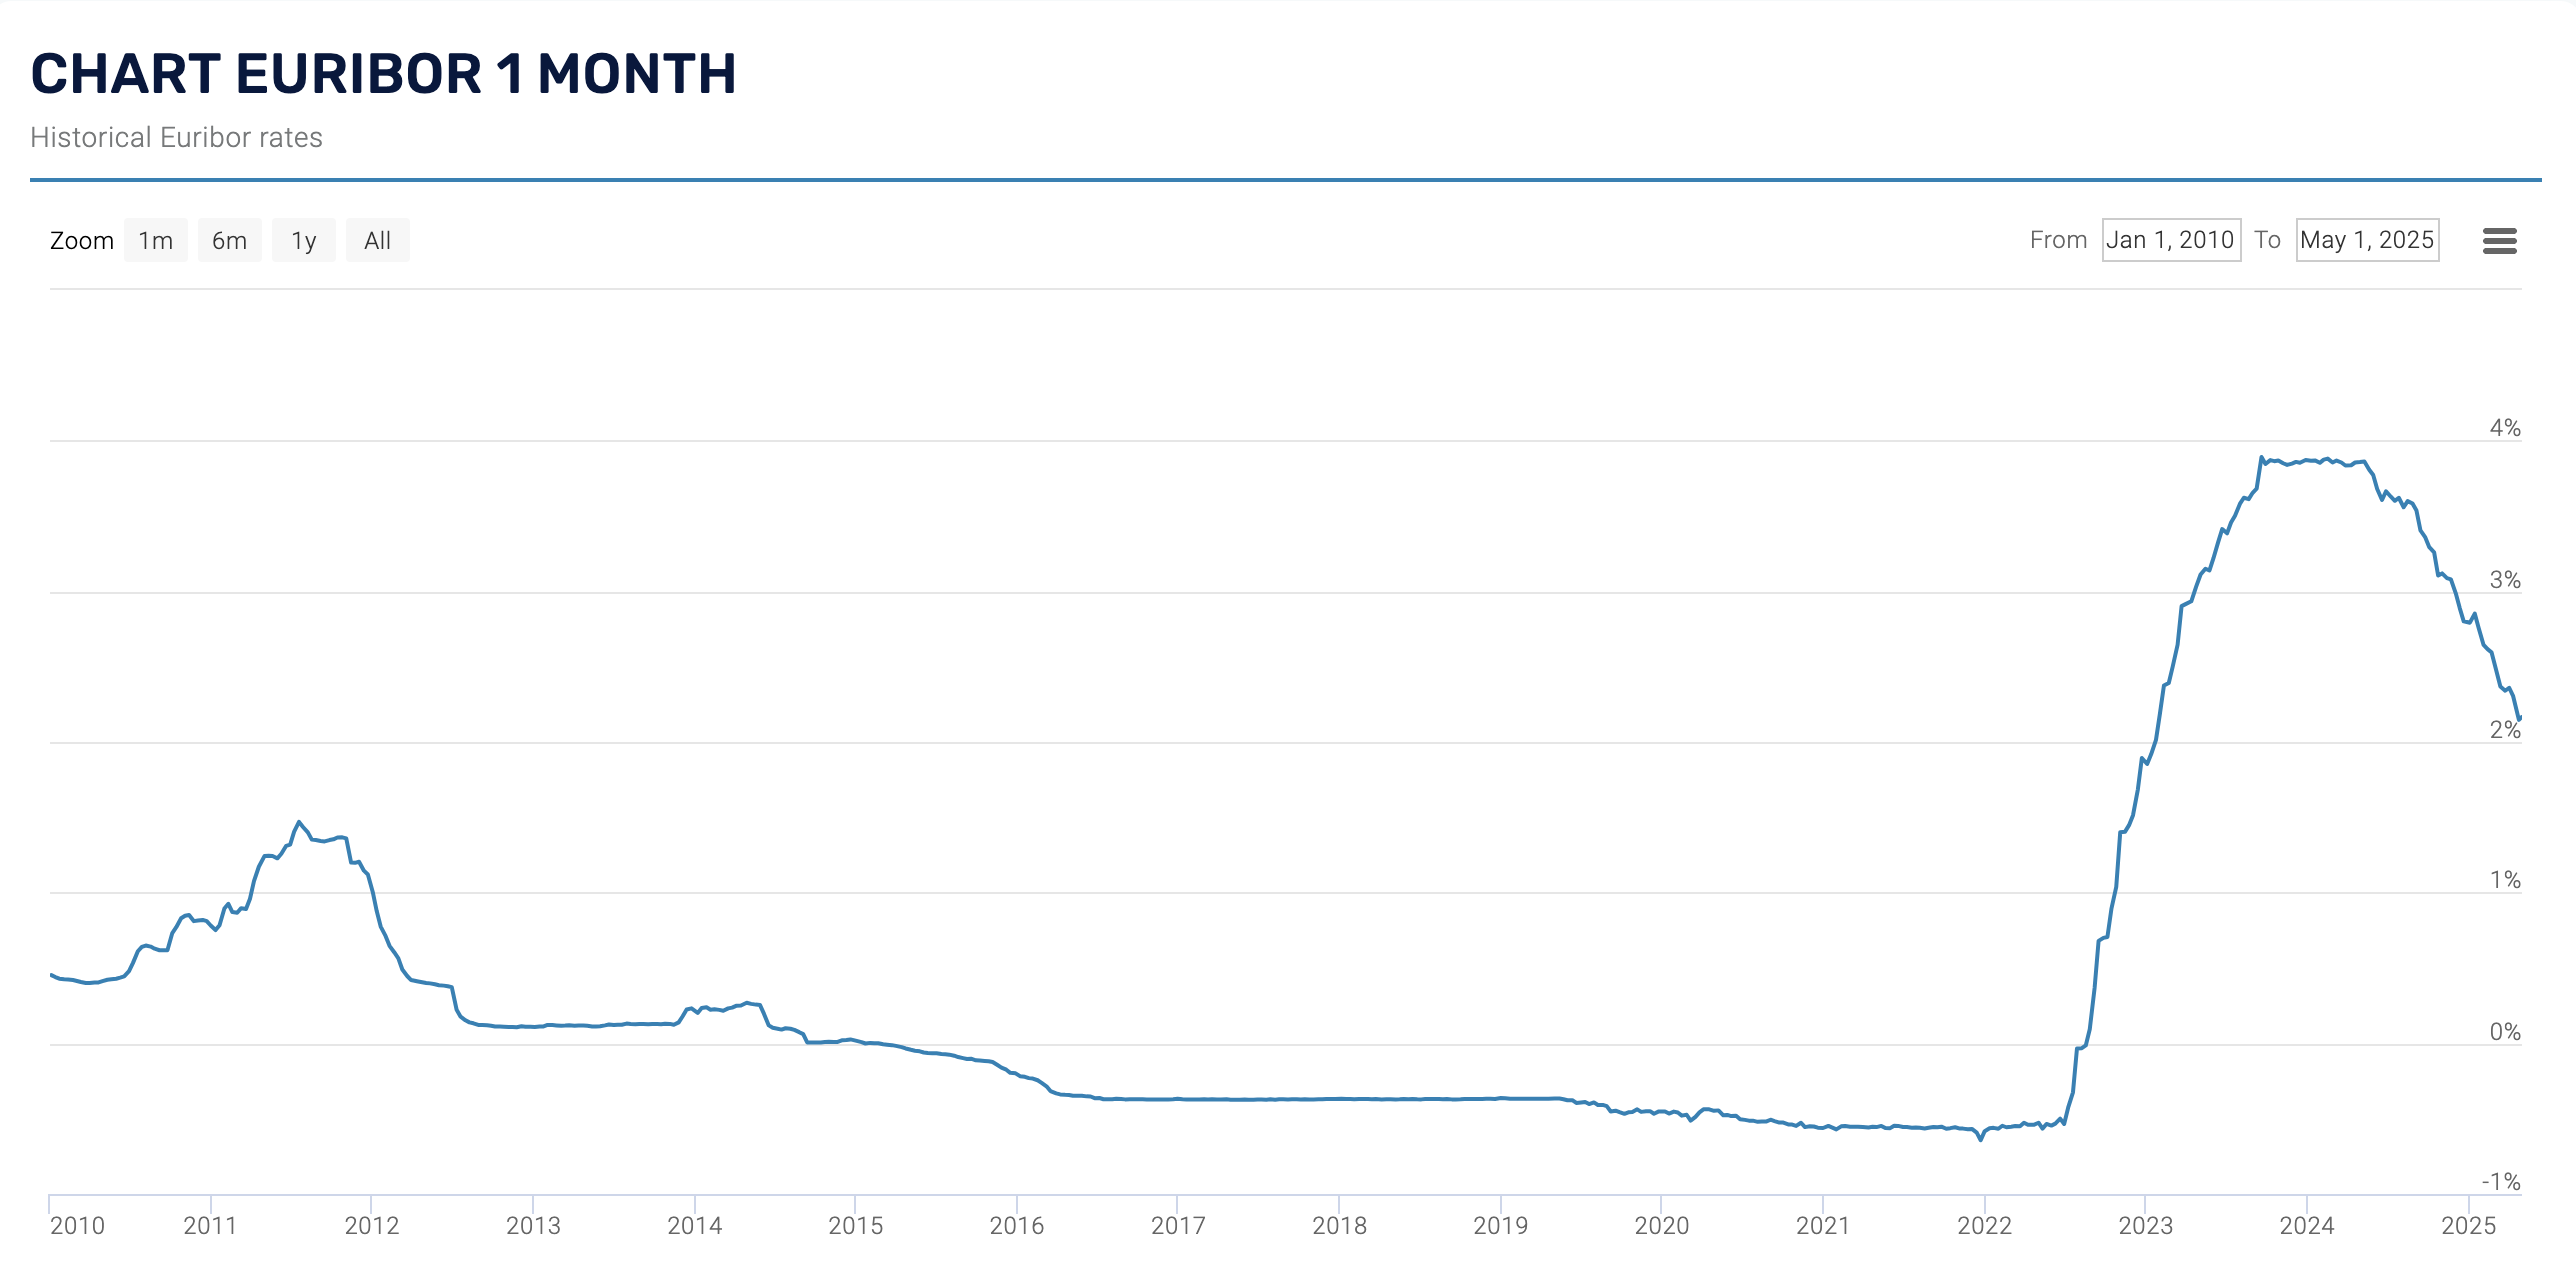
\includegraphics[width=1\linewidth]{images/macros/Euribor.png}
    \caption{\acrshort{emmi} - Euribor Interest Rates}
    \label{fig:euribor}
\end{figure}

\noindent Comparing the interest rates between 2015--2020 and 2020--2025, we can see that the first period was at a historical low, so there could be more companies with higher debt rates than normal. Some central banks, particularly in Europe, experimented with negative interest rate policies on deposit facilities during this period (figure~\ref{fig:euribor}), \cite{euribor_emmi}. This possibility should be studied in more detail, but knowing that this does not happen for the dataset between 2020--2025 where interest rates are higher, we have a clue that this could be whats causing it (see appendix figure~\ref{fig:past_scores_deep}).

\vspace{0.5cm}
\noindent Finishing with quality, there is a \textit{``defect''} in the dataset. We do not have 10 year averages for the companies that are in the 2015--2020 period --Tweenvest only has data after 2012-- so the algorithm gives 0 to some of its criteria making the maximum quality be 80. But since this is happening for all of the companies, \textbf{it is not a problem for the model fitting}, and we could easily rescale to 100.

\vspace{0.5cm}
\noindent Continuing with \textbf{growth score}, we notice that there are many companies saturating the score at 0 and 100, and the same happens with the Dividend. But looking at the deeper plots, we can see that it is closer to a uniform distribution with a descend slope after 65, which means that most companies have a similar growth rate, but fewer have higher ones.

\vspace{0.5cm}
\noindent When looking at the \textbf{value score}, we can see that the distribution almost has an average of 50, and there is a continuum of values trough the whole range decreasing as the score diverges from that average, so it seems that it is a good scale for distributing the companies.

\vspace{0.5cm}
\noindent Lastly for the \textbf{dividend score}, as mentioned before, there are many companies that do not pay dividends. But aside from that, we have an irregular distribution for the score, with a peak around 85--92 meaning that there are several companies that care about their dividend policy.

\vspace{0.5cm}
\noindent \textit{\textbf{Note}: We get very similar distributions for the Small Data datasets, but with lower resolutions of the scores distributions due to the sampling process (see appendix figures~\ref{fig:small_future_scores} and~\ref{fig:small_future_scores_deep}).}

\subsubsection{Dummies}

We have already explored the scores, so now we have to see if there distributions of the dummies could be affecting the model fitting. We started looking at the sectors distributions for the \textit{Big Data Future} to see what is full picture of the market, and then we will look at the \textit{Small Data Future} dataset since it will be the most used one in the analysis.

\begin{figure}[H]
    \centering
    \begin{minipage}{0.48\textwidth}
        \centering
        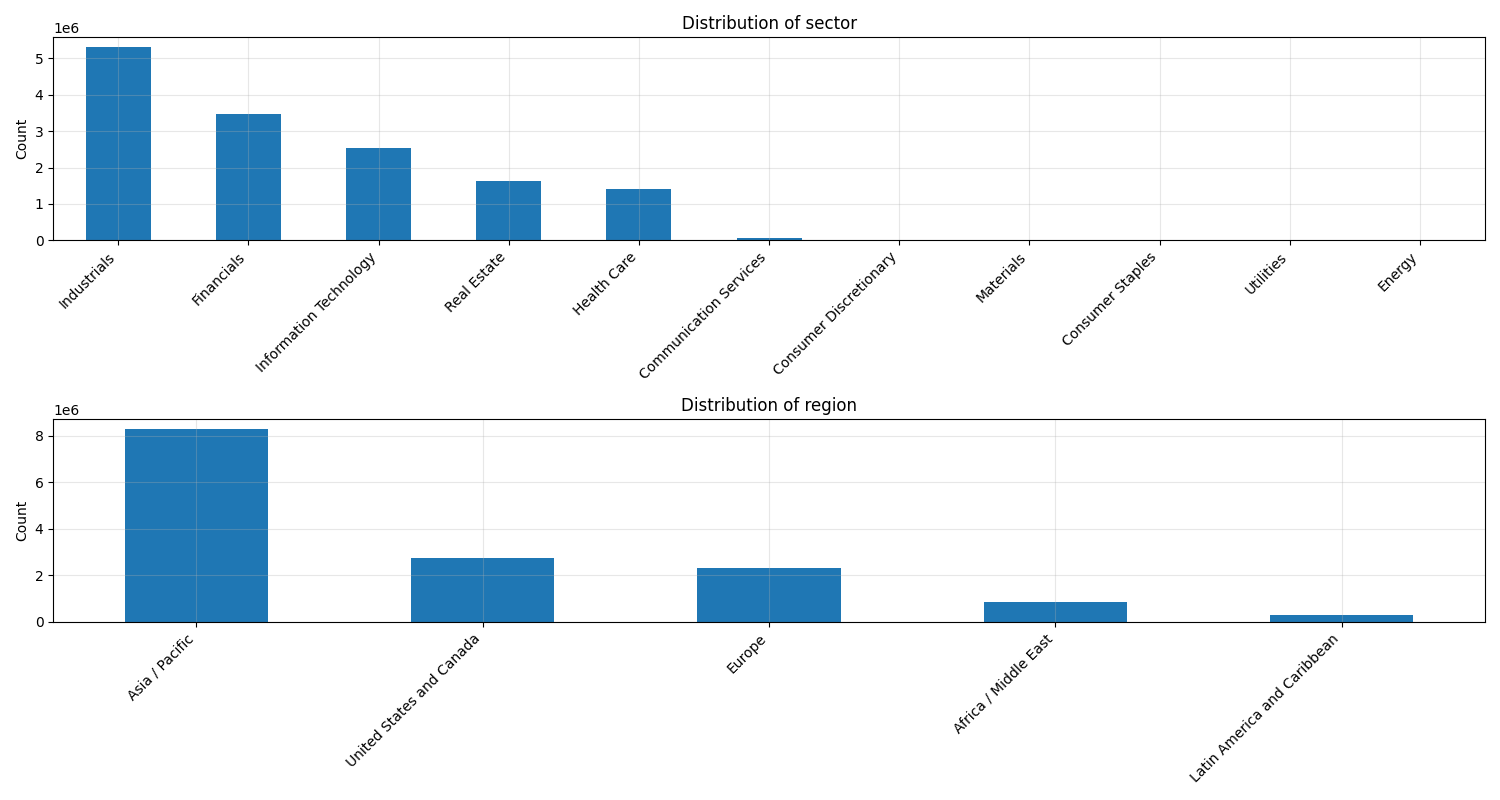
\includegraphics[width=1\linewidth]{images/code/descriptive analysis/distributions/Big Data future - Dummies.png}
        \caption{Big Data Future (\acrshort{iqr}) - Dummies}
        \label{fig:big_future_dummies}
    \end{minipage}\hfill
    \begin{minipage}{0.48\textwidth}
        \centering
        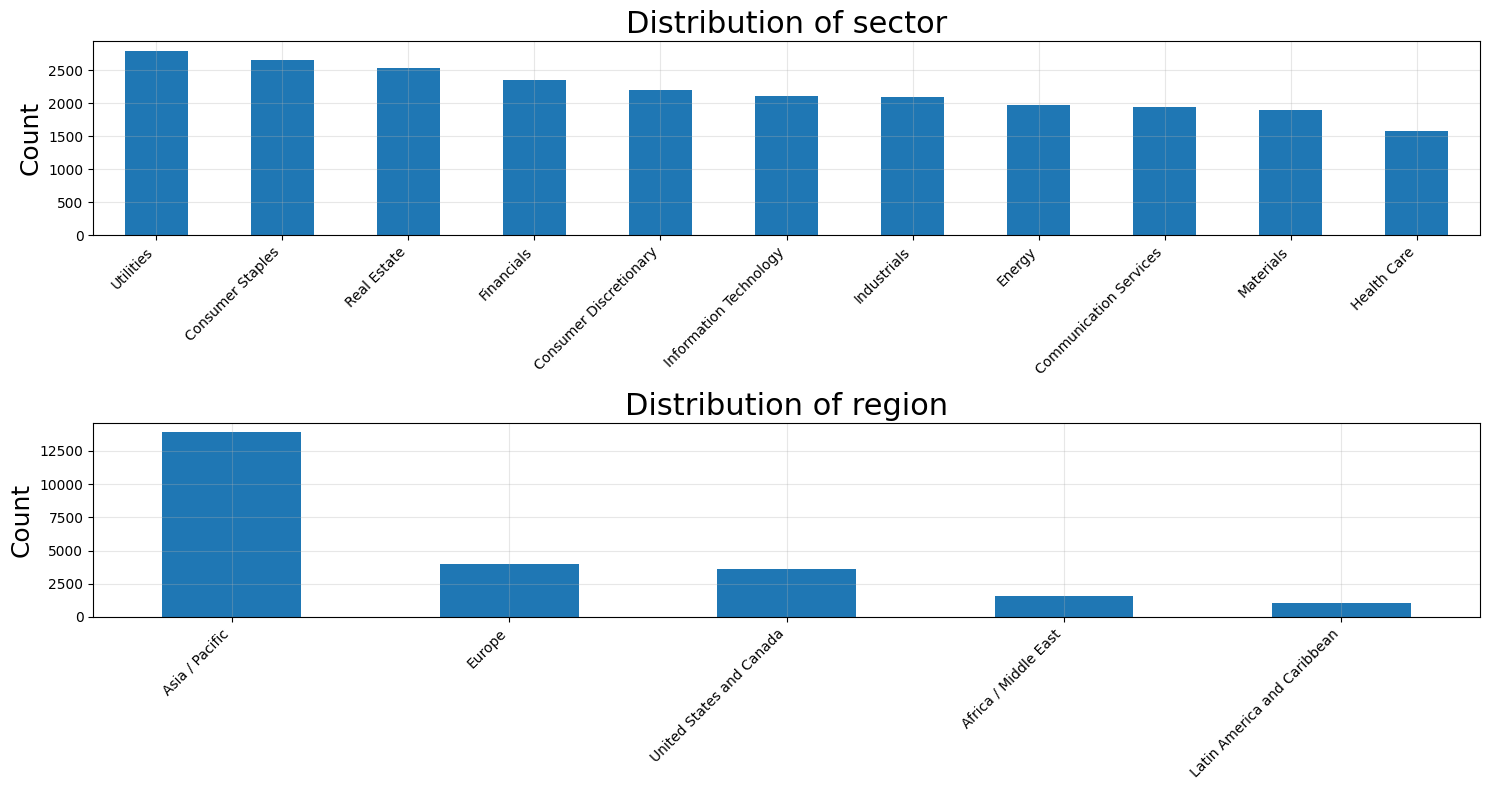
\includegraphics[width=1\linewidth]{images/code/descriptive analysis/distributions/Small Data future MCOD - Dummies.png}
        \caption{Small Data Future (\acrshort{multi}) - Dummies}
        \label{fig:small_future_dummies}
    \end{minipage}
\end{figure}

\noindent As it was expected, in figure~\ref{fig:small_future_dummies} we see a \textbf{uniform distribution for the sectors} because this condition was forced in the data creation process, but in the full dataset we have a different distribution, which could show some interesting information about how the market behaves. This made us also check the distributions for the past datasets (see appendix figures~\ref{fig:past_dummies}) where we saw a noticeable difference. This \textbf{temporal variation in sector representation} presents an interesting opportunity for future research. When it comes to the regions variables, we have a different result, seeing a \textbf{clear predomination of the Asiatic region}, which happens for all of the datasets. 

\vspace{0.5cm}
\noindent This could create issues for the model fitting, since it is known that in countries like China have more volatility and lower returns~\cite{chen2024economic}. Also, their auditors often lack true independence, especially when auditing \gls{soe} or firms with strong political ties. The Chinese government tightly controls domestic accounting firms and imposes restrictions on foreign auditors. Even international firms like \textit{PwC-China} operate under local joint ventures, often with limited autonomy, as reviewed in~\cite{LIU2012782}. So we will have to check if the dummies variables are enough to take this effect into account, or if we need a different approach for modeling the geographical effects.

\subsubsection{Profits}

\noindent Finally, when analyzing the profit distributions across different time horizons, we observe that the distributions contain a numerous amount of outliers that do not let us see the distributions clearly (appendix figures~\ref{fig:big_data_future_profits_boxplot} and~\ref{fig:big_data_future_profits}).

\begin{figure}[H]
    \centering
    \begin{minipage}{0.5\textwidth}
        \centering
        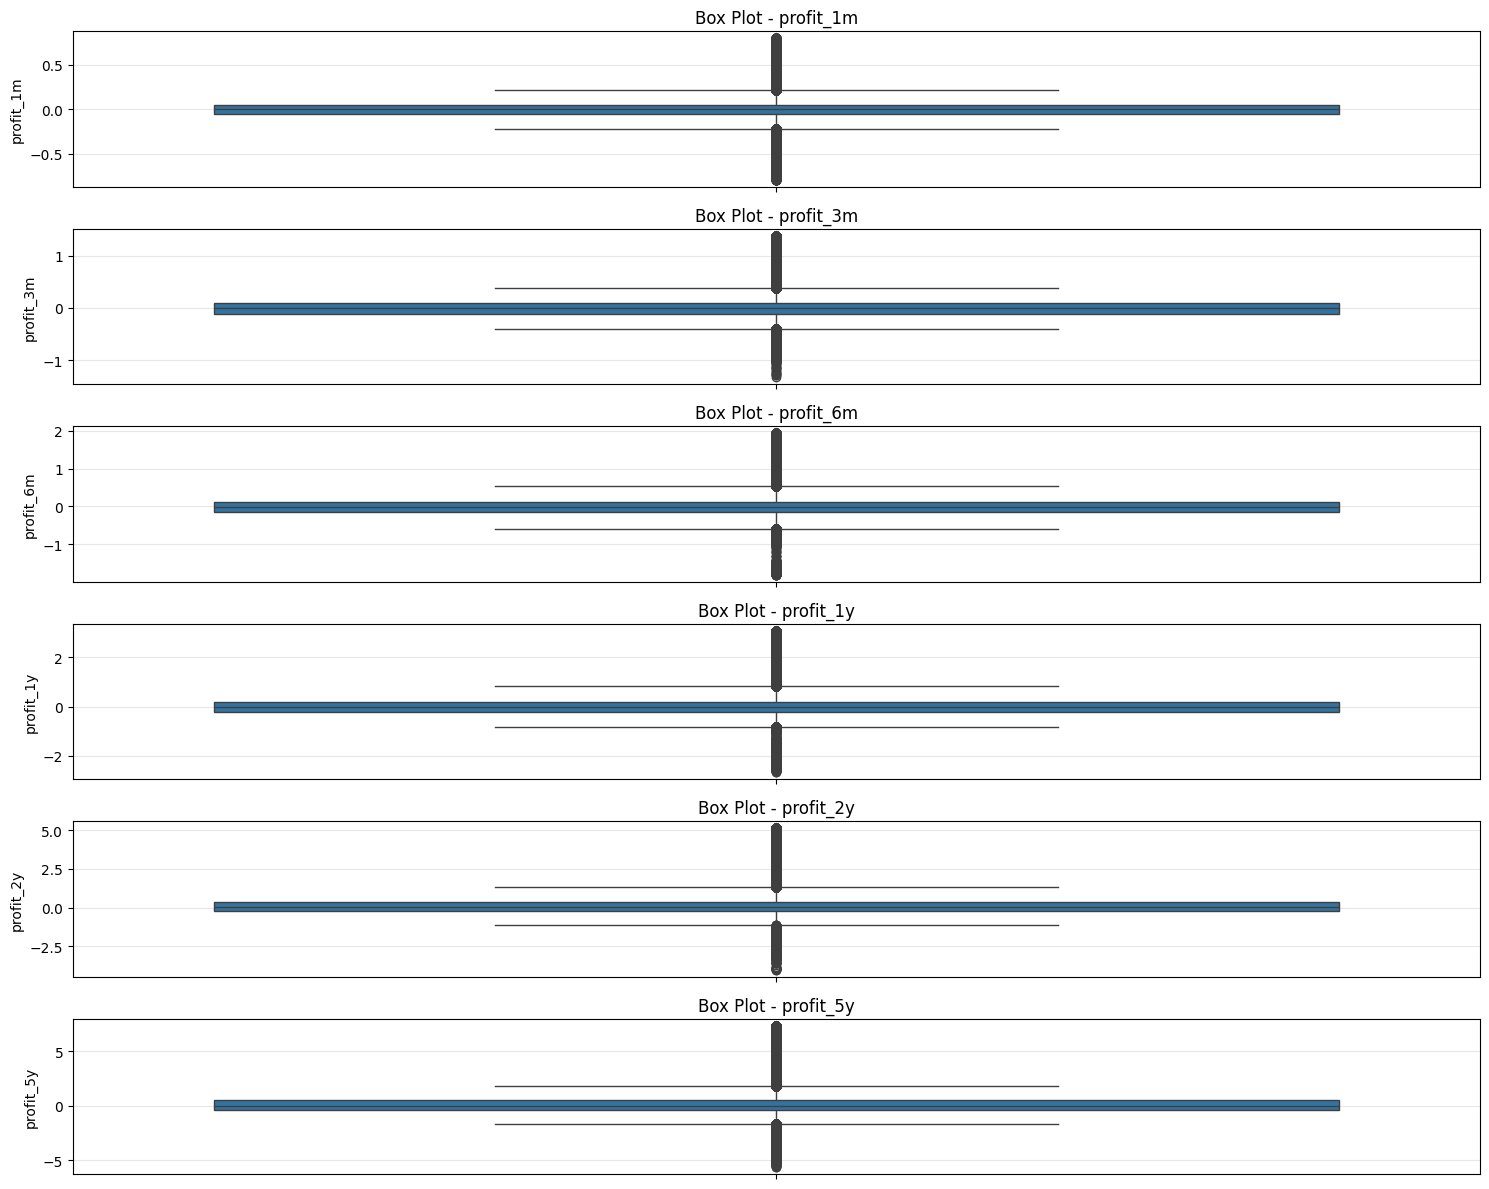
\includegraphics[width=1\linewidth]{images/code/descriptive analysis/distributions/Big Data future IQR - Profits Boxplot.png}
        \caption{Big Data Future \acrshort{iqr} - Profits Boxplot}
        \label{fig:big_data_future_iqr_profits_boxplot}
    \end{minipage}\hfill
    \begin{minipage}{0.5\textwidth}
        \centering
        \includegraphics[width=1\linewidth]{images/code/descriptive analysis/distributions/Big Data Future IQR - Profits.png}
        \caption{Big Data Future \acrshort{iqr} - Profits}
        \label{fig:big_data_future_iqr_profits_iqr}
    \end{minipage}
\end{figure}

\noindent Interestingly, we notice that the \textbf{short-term profit} distributions (1-month and 3-month) are more symmetric and closer to \textbf{normal distributions}, which is consistent with the efficient market hypothesis suggesting that short-term price movements are largely random. However, as we extend to \textbf{longer time horizons}, the \textbf{distributions become more positively skewed}, which aligns with the general expectation that most companies do not have good returns, except of the market winners that tend to generate extraordinary positive returns due to the mentioned \textbf{\textit{economic moats}}. This is particularly evident in the longer-term profit distributions (2-year and 5-year), where we see a \textbf{longer tail extending toward higher positive returns}. Finally, there is also a tendency to having \textbf{less negative returns} compared to the positive ones the longer the time-frame. Logically, companies with bad returns do not last long.

\subsection{Correlations}

For analyzing the correlations between the variables, we will start firstly with just the cleaned big datasets, and then we will use also the datasets without the outliers using the multi-variate approach explained in previous chapters, since these are the ones that will be used for the model fitting in most of the analysis. We have to make clear that this is the last section where \textbf{we will be using the past datasets}, to see if past profits are being reflected in current scores.

\subsubsection{Clean Datasets}
\begin{figure}[H]
    \centering
    \begin{minipage}{0.48\textwidth}
        \centering
        \includegraphics[width=\linewidth]{images/code/descriptive analysis/correlations/Big Data Past.png}
        \caption{Big Data Past (Clean) - Correlations}
        \label{fig:big_data_past_correlations}
    \end{minipage}\hfill
    \begin{minipage}{0.48\textwidth}
        \centering
        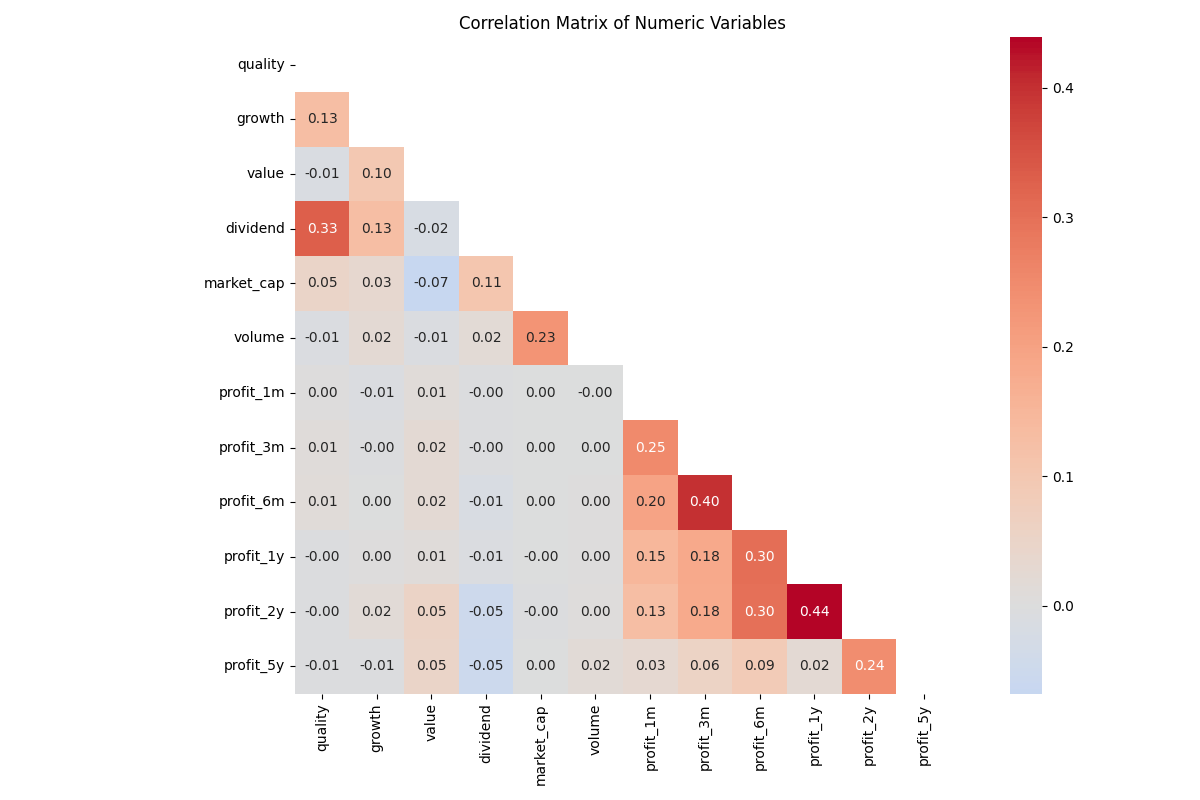
\includegraphics[width=\linewidth]{images/code/descriptive analysis/correlations/Big Data future.png}
        \caption{Big Data Future (Clean) - Correlations}
        \label{fig:big_data_future_correlations}
    \end{minipage}
\end{figure}

\noindent We can appreciate three main expected correlations:
\begin{itemize}
    \item \textbf{Companies with good quality} --that is so, they have consistent growth, good liquidity and healthy debt-- \textbf{are more likely to give dividends}.
    \item There is a strong relationship between the market cap of a stock and the volume of the shares traded.
    \item \textbf{Companies have inertia}, or how it is mostly called \textit{Momentum}, meaning that the profit of a company is positively correlated with the profit of the previous period.
\end{itemize}

\subsubsection{Outliers Datasets}
\begin{figure}[H]
    \centering
    \begin{minipage}{0.48\textwidth}
        \centering
        \includegraphics[width=\linewidth]{images/code/descriptive analysis/correlations/Big Data Past - IF.png}
        \caption{Big Data Past \acrshort{if} (4\%) - Correlations}
        \label{fig:big_data_past_if_correlations}
    \end{minipage}\hfill
    \begin{minipage}{0.48\textwidth}
        \centering
        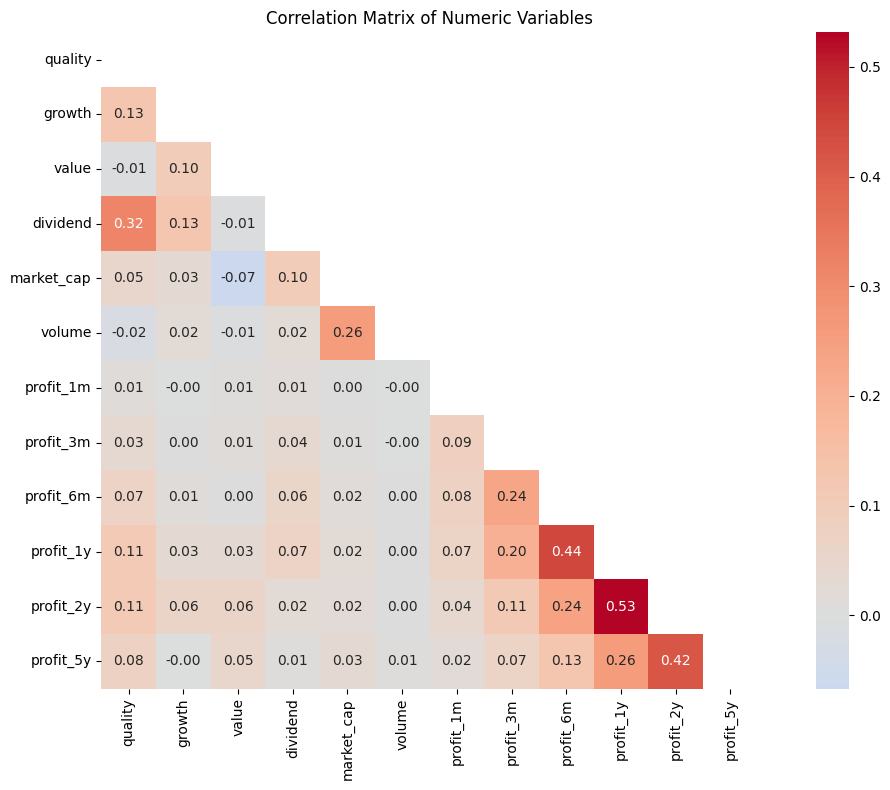
\includegraphics[width=\linewidth]{images/code/descriptive analysis/correlations/Big Data future - IF.png}
        \caption{Big Data Future \acrshort{if} (4\%) - Correlations}
        \label{fig:big_data_future_if_correlations}
    \end{minipage}
\end{figure}

\noindent For getting a bigger picture we only used a small outlier removal. And as expected, the correlations already seen before any removal stay similar with a slight increase in the \textit{Momentum}, showing more importance of it than other variables. But actually, there are \textbf{new correlations seen} for both datasets:

\begin{itemize}
    \item  \textbf{Accumulated profits affect the scores}. In the past dataset we can see that long term past profits translate into higher growth, quality and dividend scores, these were expected to increase together due to their correlation. But also, we see that \textbf{accumulated stock performance make the value score decrease}. This could be explained by two effects:
    \begin{itemize}
        \item \textbf{Bull markets}. As explained in the second chapter, a company can experience returns in the stock market that cannot be followed by financial growth. This makes their value multiples to raise, making their value score to decrease.
        \item \textbf{Unknown companies}. There is a possibility that the company is not well known, so the market price is lower than it could while their finances are good. This hypothesis could be supported if Value score is correlated to future market profits, which we will see soon.
    \end{itemize}
    \item \textbf{Long term stock returns affect the company's growth}. This is a very interesting result, since it explains the reason why companies try to go to the market to raise capital and help the company grow.
    \item \textbf{Quality is correlated to future profits}. This could be explained by the fact that a company with good quality is more likely to have good future profits, but also by the fact that the market is efficient and the price of a company will reflect all of the information available.
    \item There is a \textbf{mild correlation between most scores}, which could be explain by the fact that a company that does well in one aspect, is more likely to do well in the others. This correlation will not affect the models because they are separated by score.
\end{itemize}

\noindent Although we have to make clear that these correlations do not stand along all of the geographical datasets (see appendix figures from~\ref{fig:small_data_future_usa_correlations} to~\ref{fig:small_data_future_as_multi_correlations}), so we cannot be sure if these correlations will be properly explained by the linear models.

\subsubsection{Validation Dataset}

\begin{figure}[H]
    \centering
    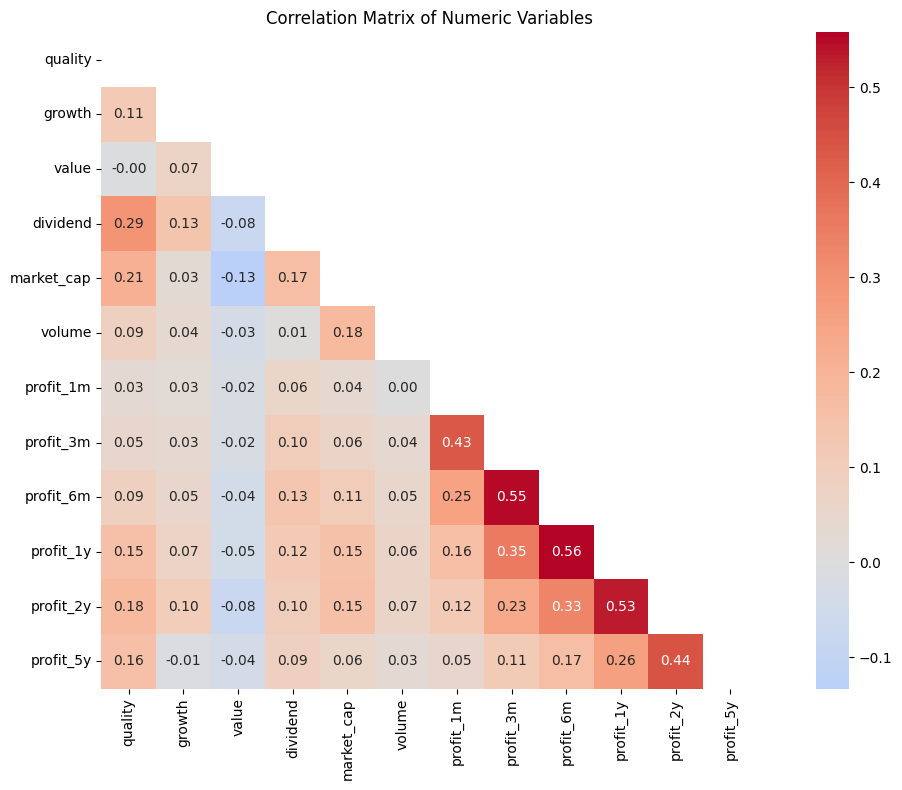
\includegraphics[width=0.48\textwidth]{images/code/descriptive analysis/correlations/Medium future - IF HARD.png}
    \caption{Medium Data Future \acrshort{if} (35\%) - Correlations}
    \label{fig:medium_data_future_if_correlations}
\end{figure}


\noindent Also, as we mentioned in the previous chapter, in figure~\ref{fig:medium_data_future_if_correlations} we see a huge increase in the previous correlations when we removed more outliers. And a new inverse correlation for \textit{Market Cap} and \textit{Value}. It is interesting that this relationship is not as strong as we could expect.

\subsection{Data clusters}
Finally, we are going to try to compare these results with the \acrshort{pairplot} of the datasets, to look for clusters of data when comparing many variables at once.

\begin{figure}[H]
    \centering
    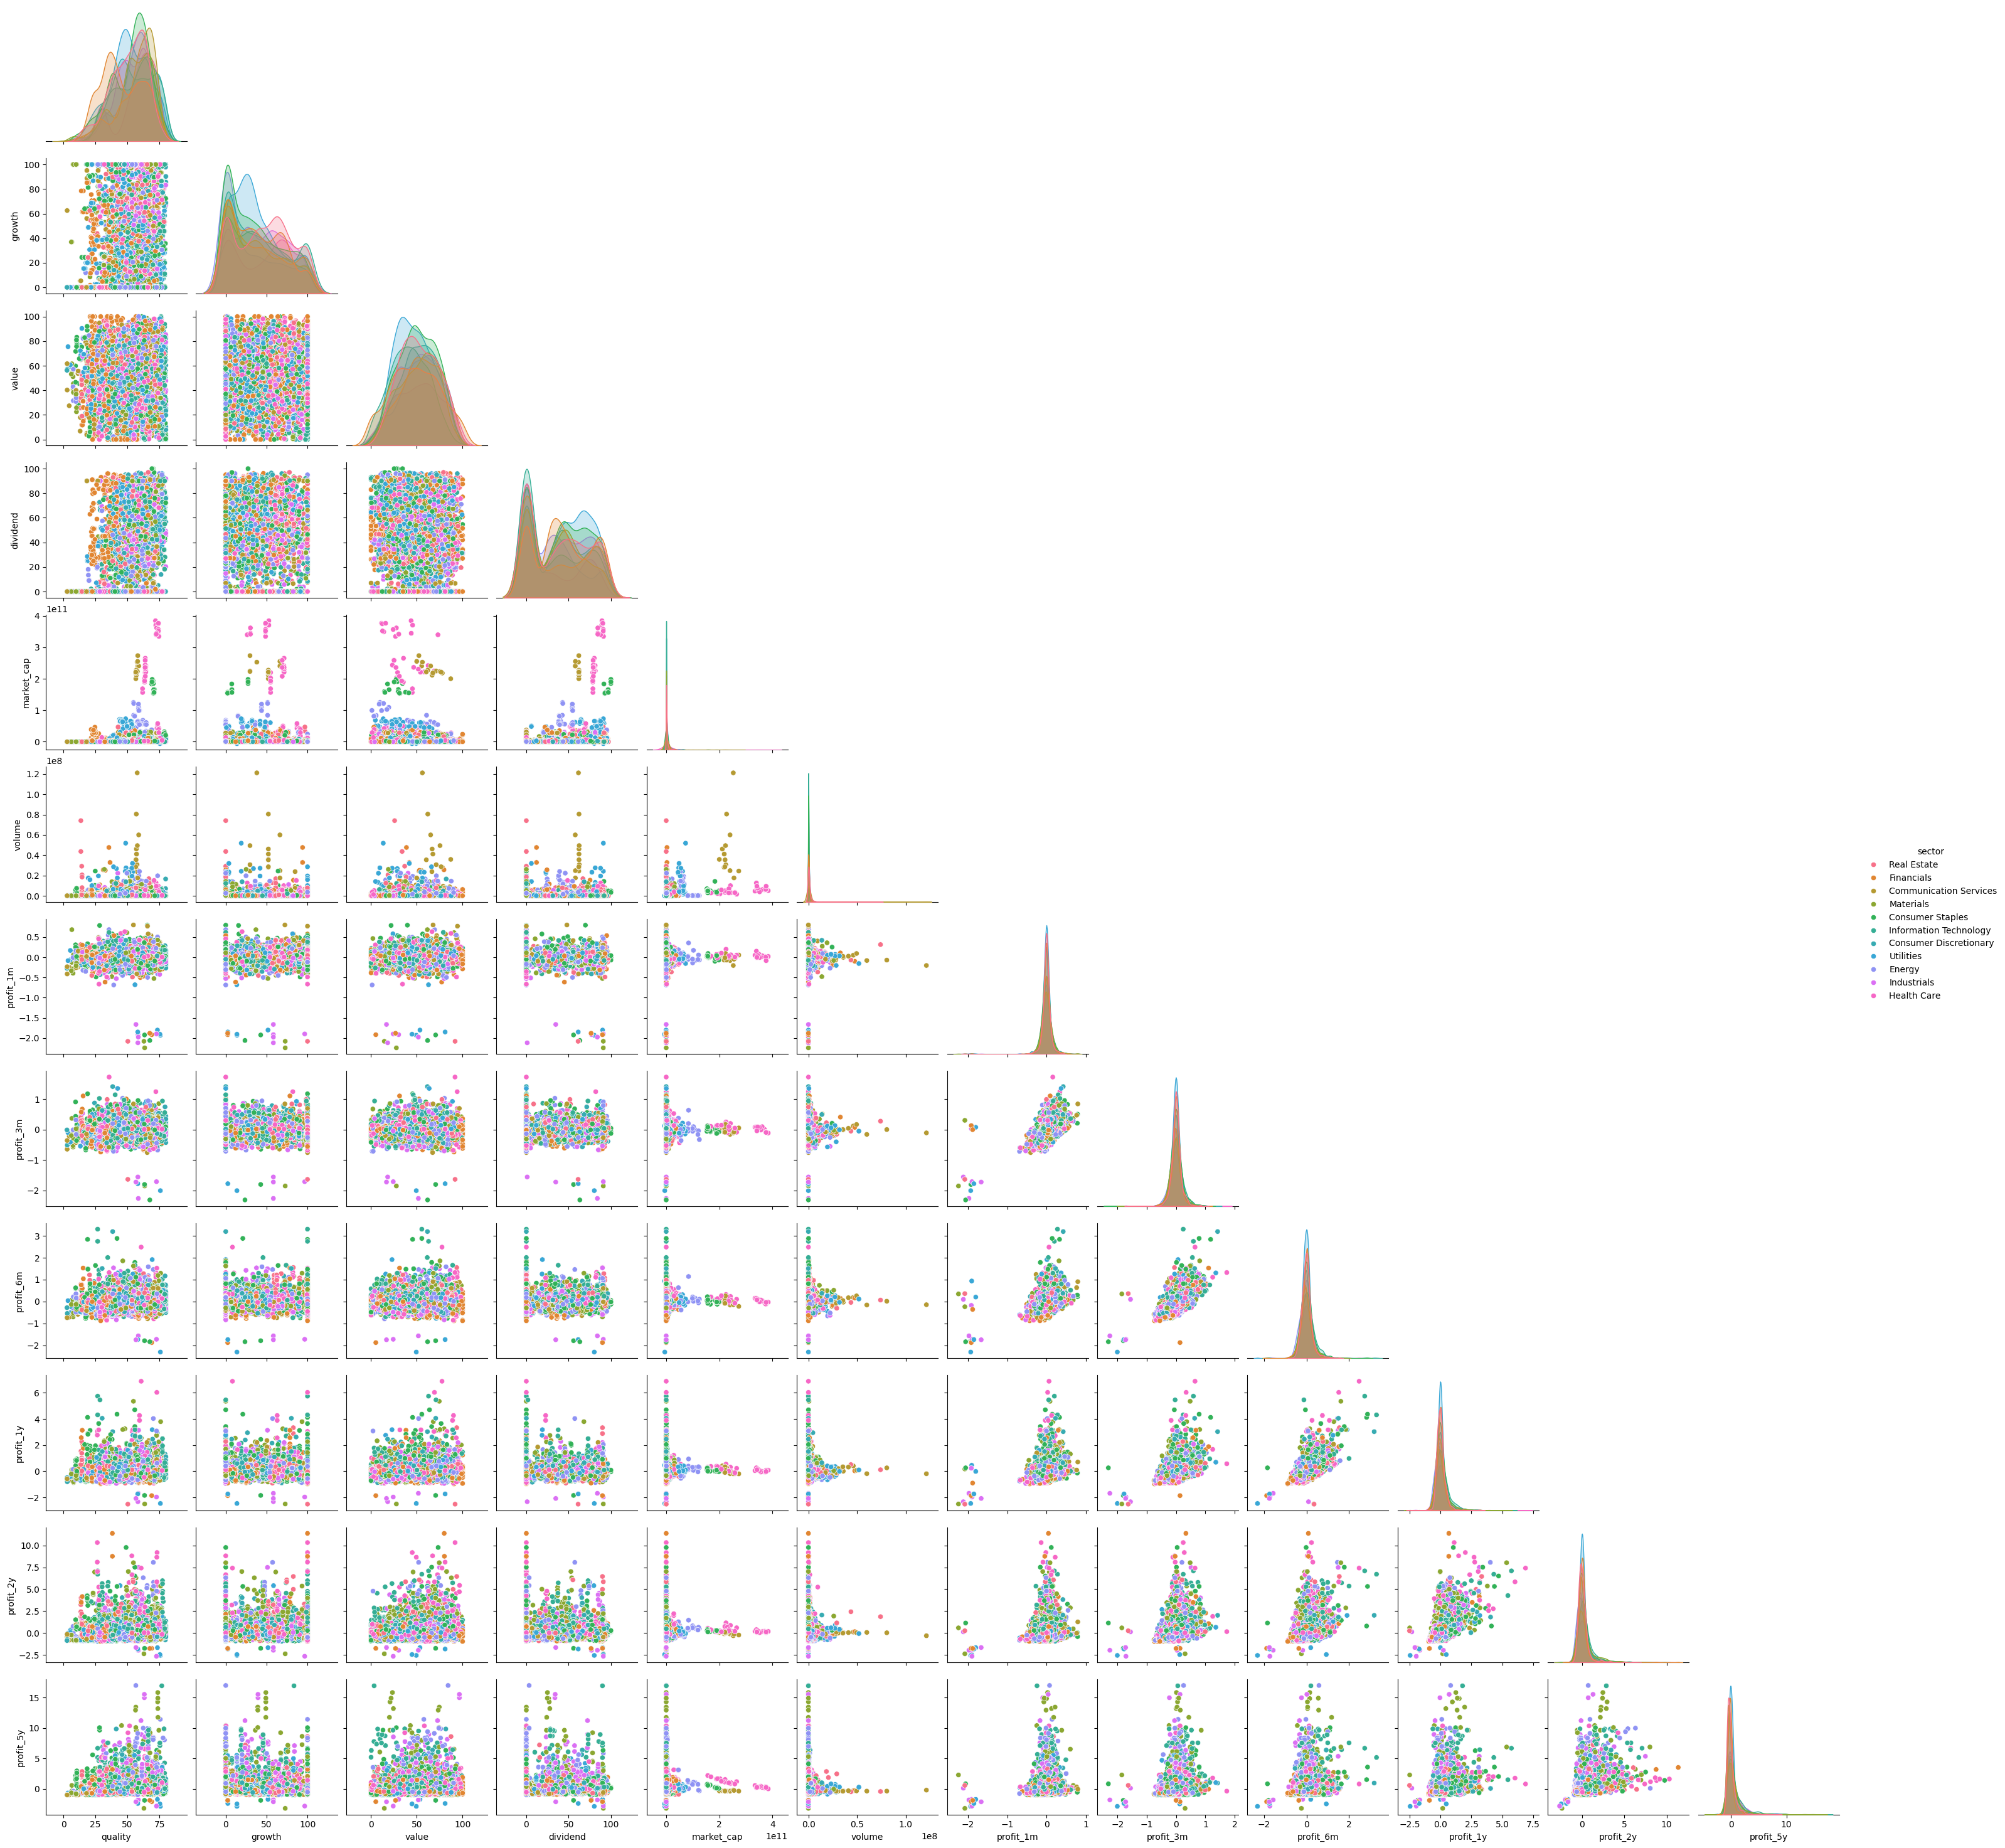
\includegraphics[width=1\textwidth]{images/code/descriptive analysis/correlations/Small Data future - Multi - pairplot.png}
    \caption{Small Data Future - \acrshort{multi} (4\%) \acrshort{pairplot}}
    \label{fig:pairplot_small_data_future_multi}
\end{figure}

\noindent Here it is harder to eye-see the data structure that could form clusters since there are many data-points, but there are some exceptions:
\begin{itemize}
    \item \textbf{Profits}. We can see linear correlations between some of the different profits, but for longer horizons the relationships are no longer linear. Which is expected since the further the horizon, more variables take part in the calculation of the profit.
    \item \textbf{\acrshort{marketcap}}. Companies with bigger market caps tend to have higher quality and dividend scores. Bigger companies should have a more stable financial situation, otherwise they would not be as big in the long term. Also there are some sectors that tend to have higher market caps than others, like \textit{Health Care} or \textit{Consumer Staples}.
    \item \textbf{Sector}. It seems that there could be a pattern seen in the sectors distribution for each scores, but it is not clear.
\end{itemize}

\noindent Although, these results are not as clear and they also variate depending on the dataset. Showing early results of non-linear relationships with the dummy variables.

\section{Predictive Models}

Now that we understand the data, and the different datasets created. We are going to explain how was the process of refining the methodologies for improving the results.

\subsection{Linear Regression}

First of all, we started with a family of simple linear regression models with very few variables and not excluding the outliers. This, of course, resulted in a very poor model that could not predict anything (see appendix figure~\ref{fig:first_linear_regression_performance}). However, after applying the first outlier removal for the initial series of datasets, we started to see some results:

\begin{figure}[H]
    \centering
    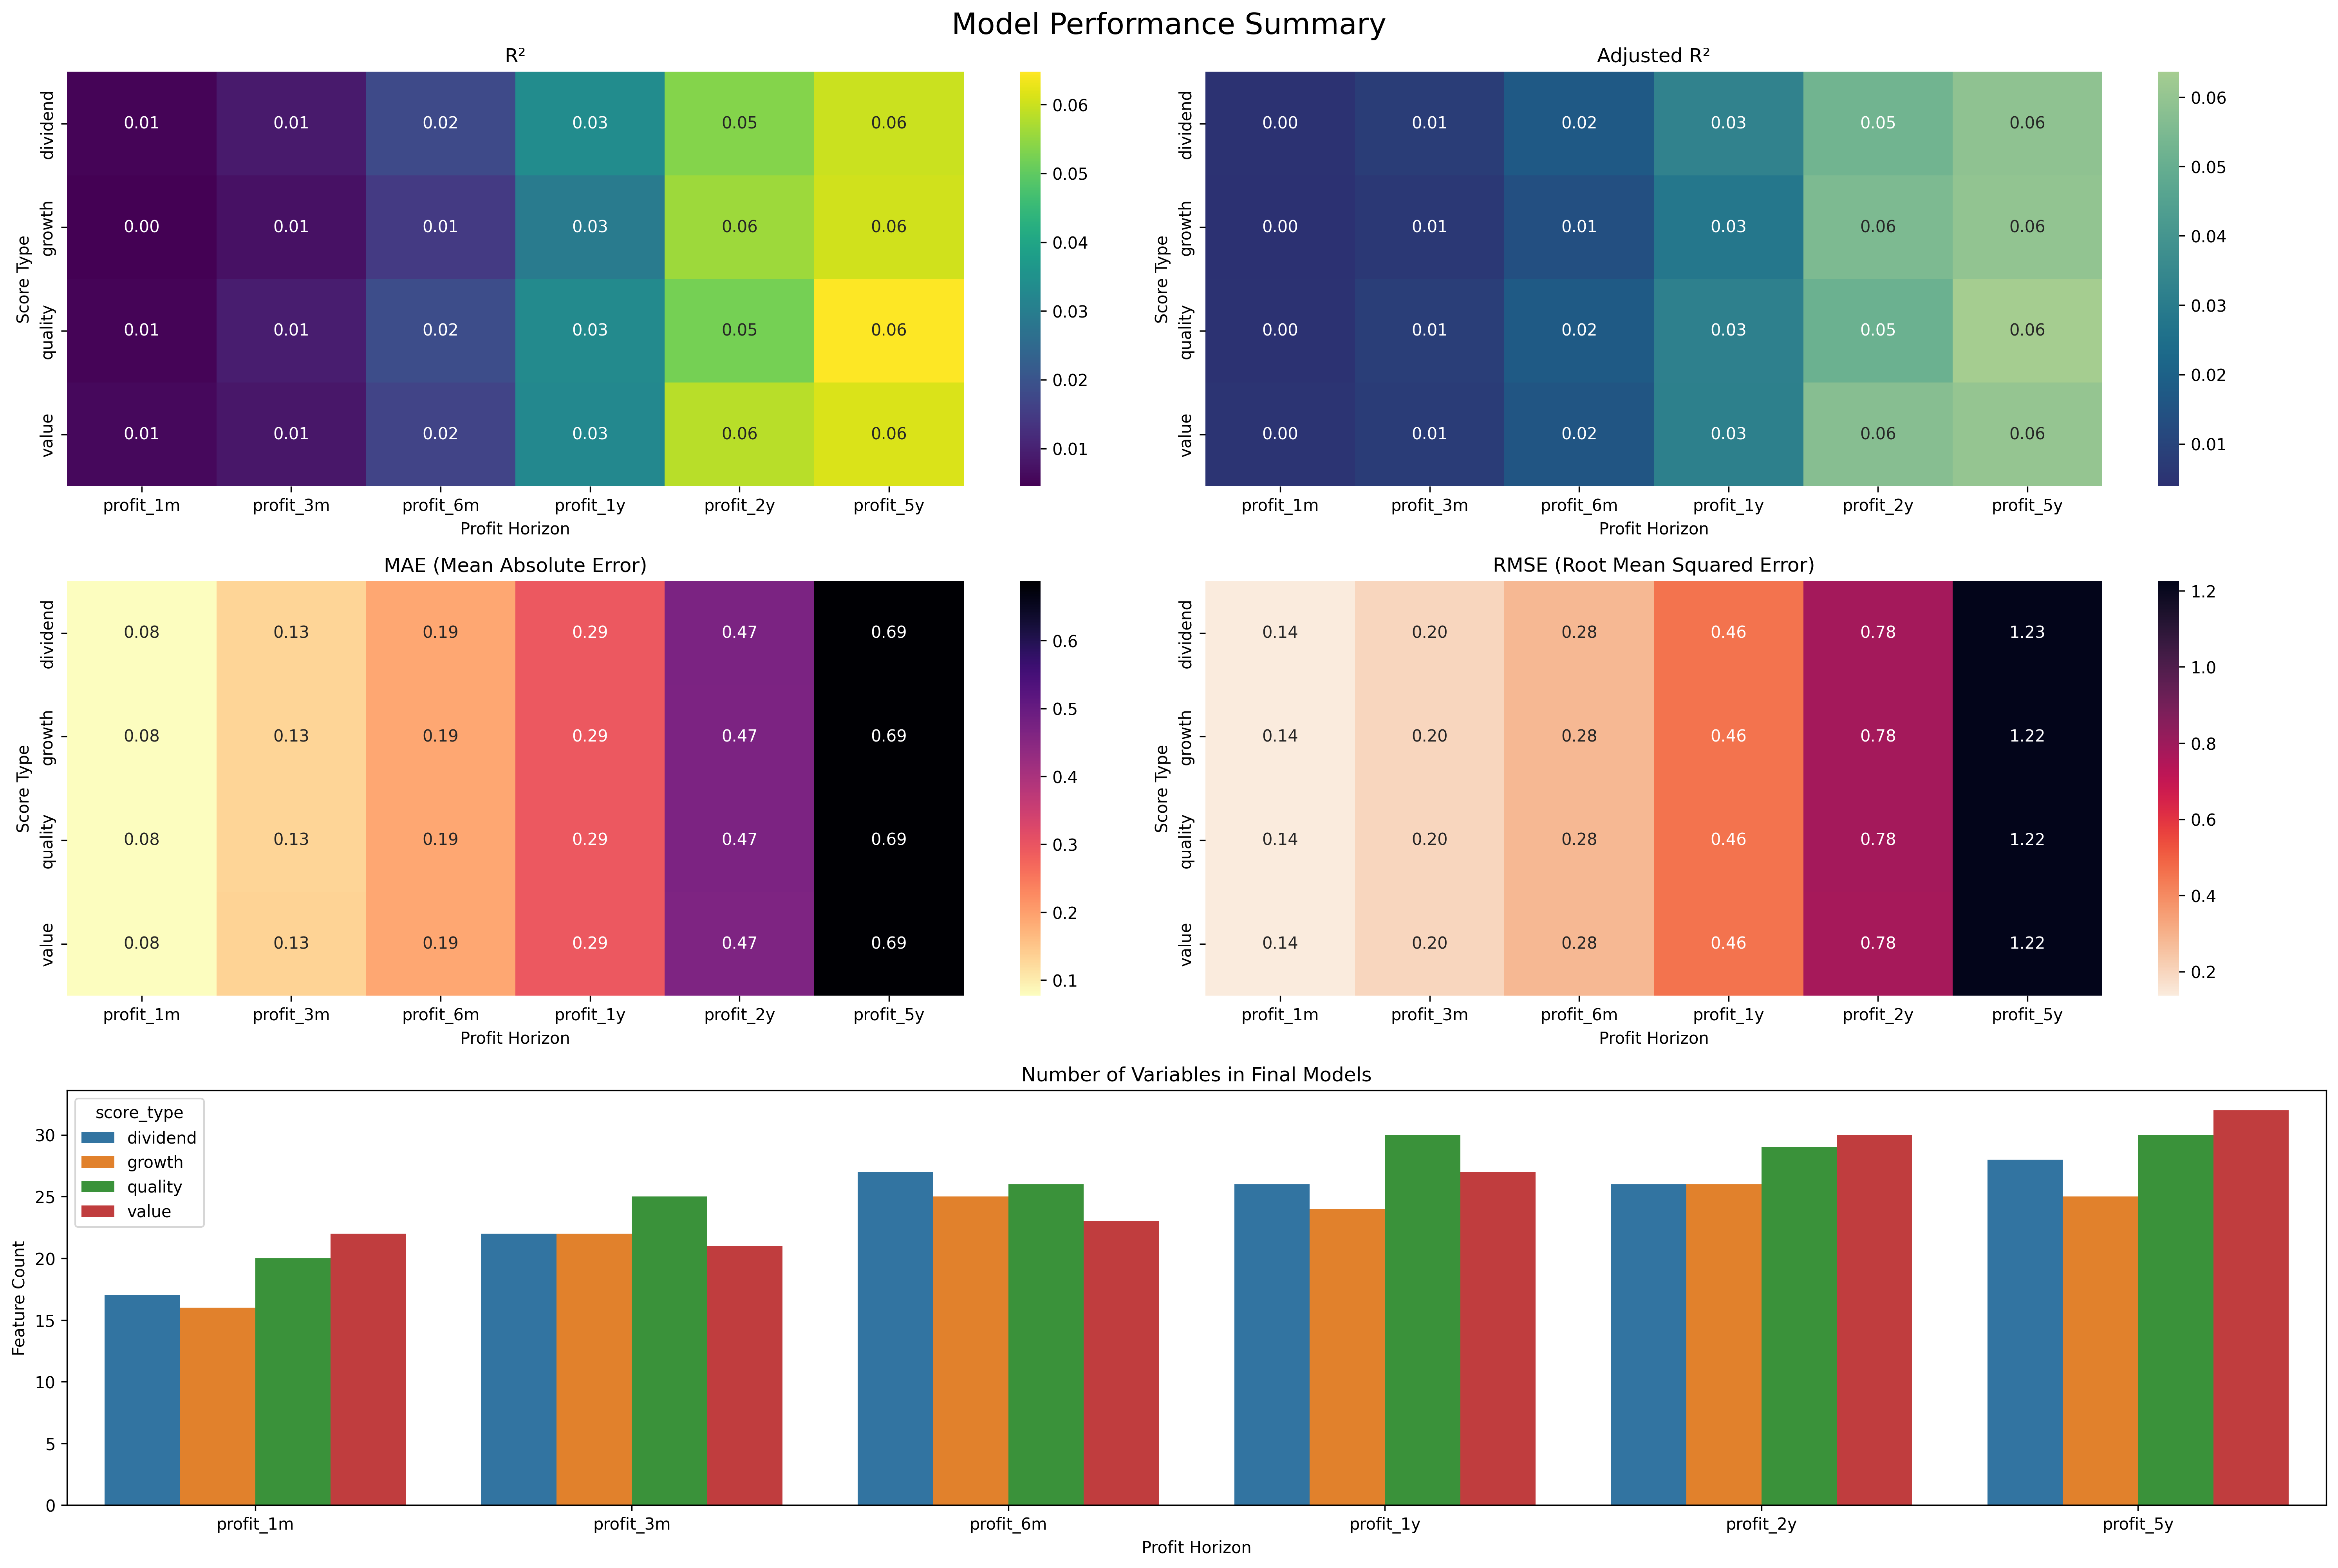
\includegraphics[width=1\textwidth]{images/code/models/linear_regression/first_model/Small Data future - Multi performance.png}
    \caption{Small Data Future - \acrshort{multi} (4\%)}
    \label{fig:first_linear_regression}
\end{figure}

\noindent In figure~\ref{fig:first_linear_regression} we observe a consistent pattern across all models: the further into the future we try to predict profits, the better the model performs in terms of capturing trends, but the prediction error also increases. This is expected, as \textbf{long-term forecasts naturally involve greater variance}; however, stable companies tend to exhibit more predictable behavior over time. Additionally, we notice that the \acrshort{rmse} is nearly twice as large as the \acrshort{mae}, which suggests the \textbf{presence of numerous outliers in the data}. Also it is worth mentioning that the number of variables increase at the same time as the models' performance improves, which could be a \textbf{sign of overfitting}.

\begin{figure}[H]
    \centering
    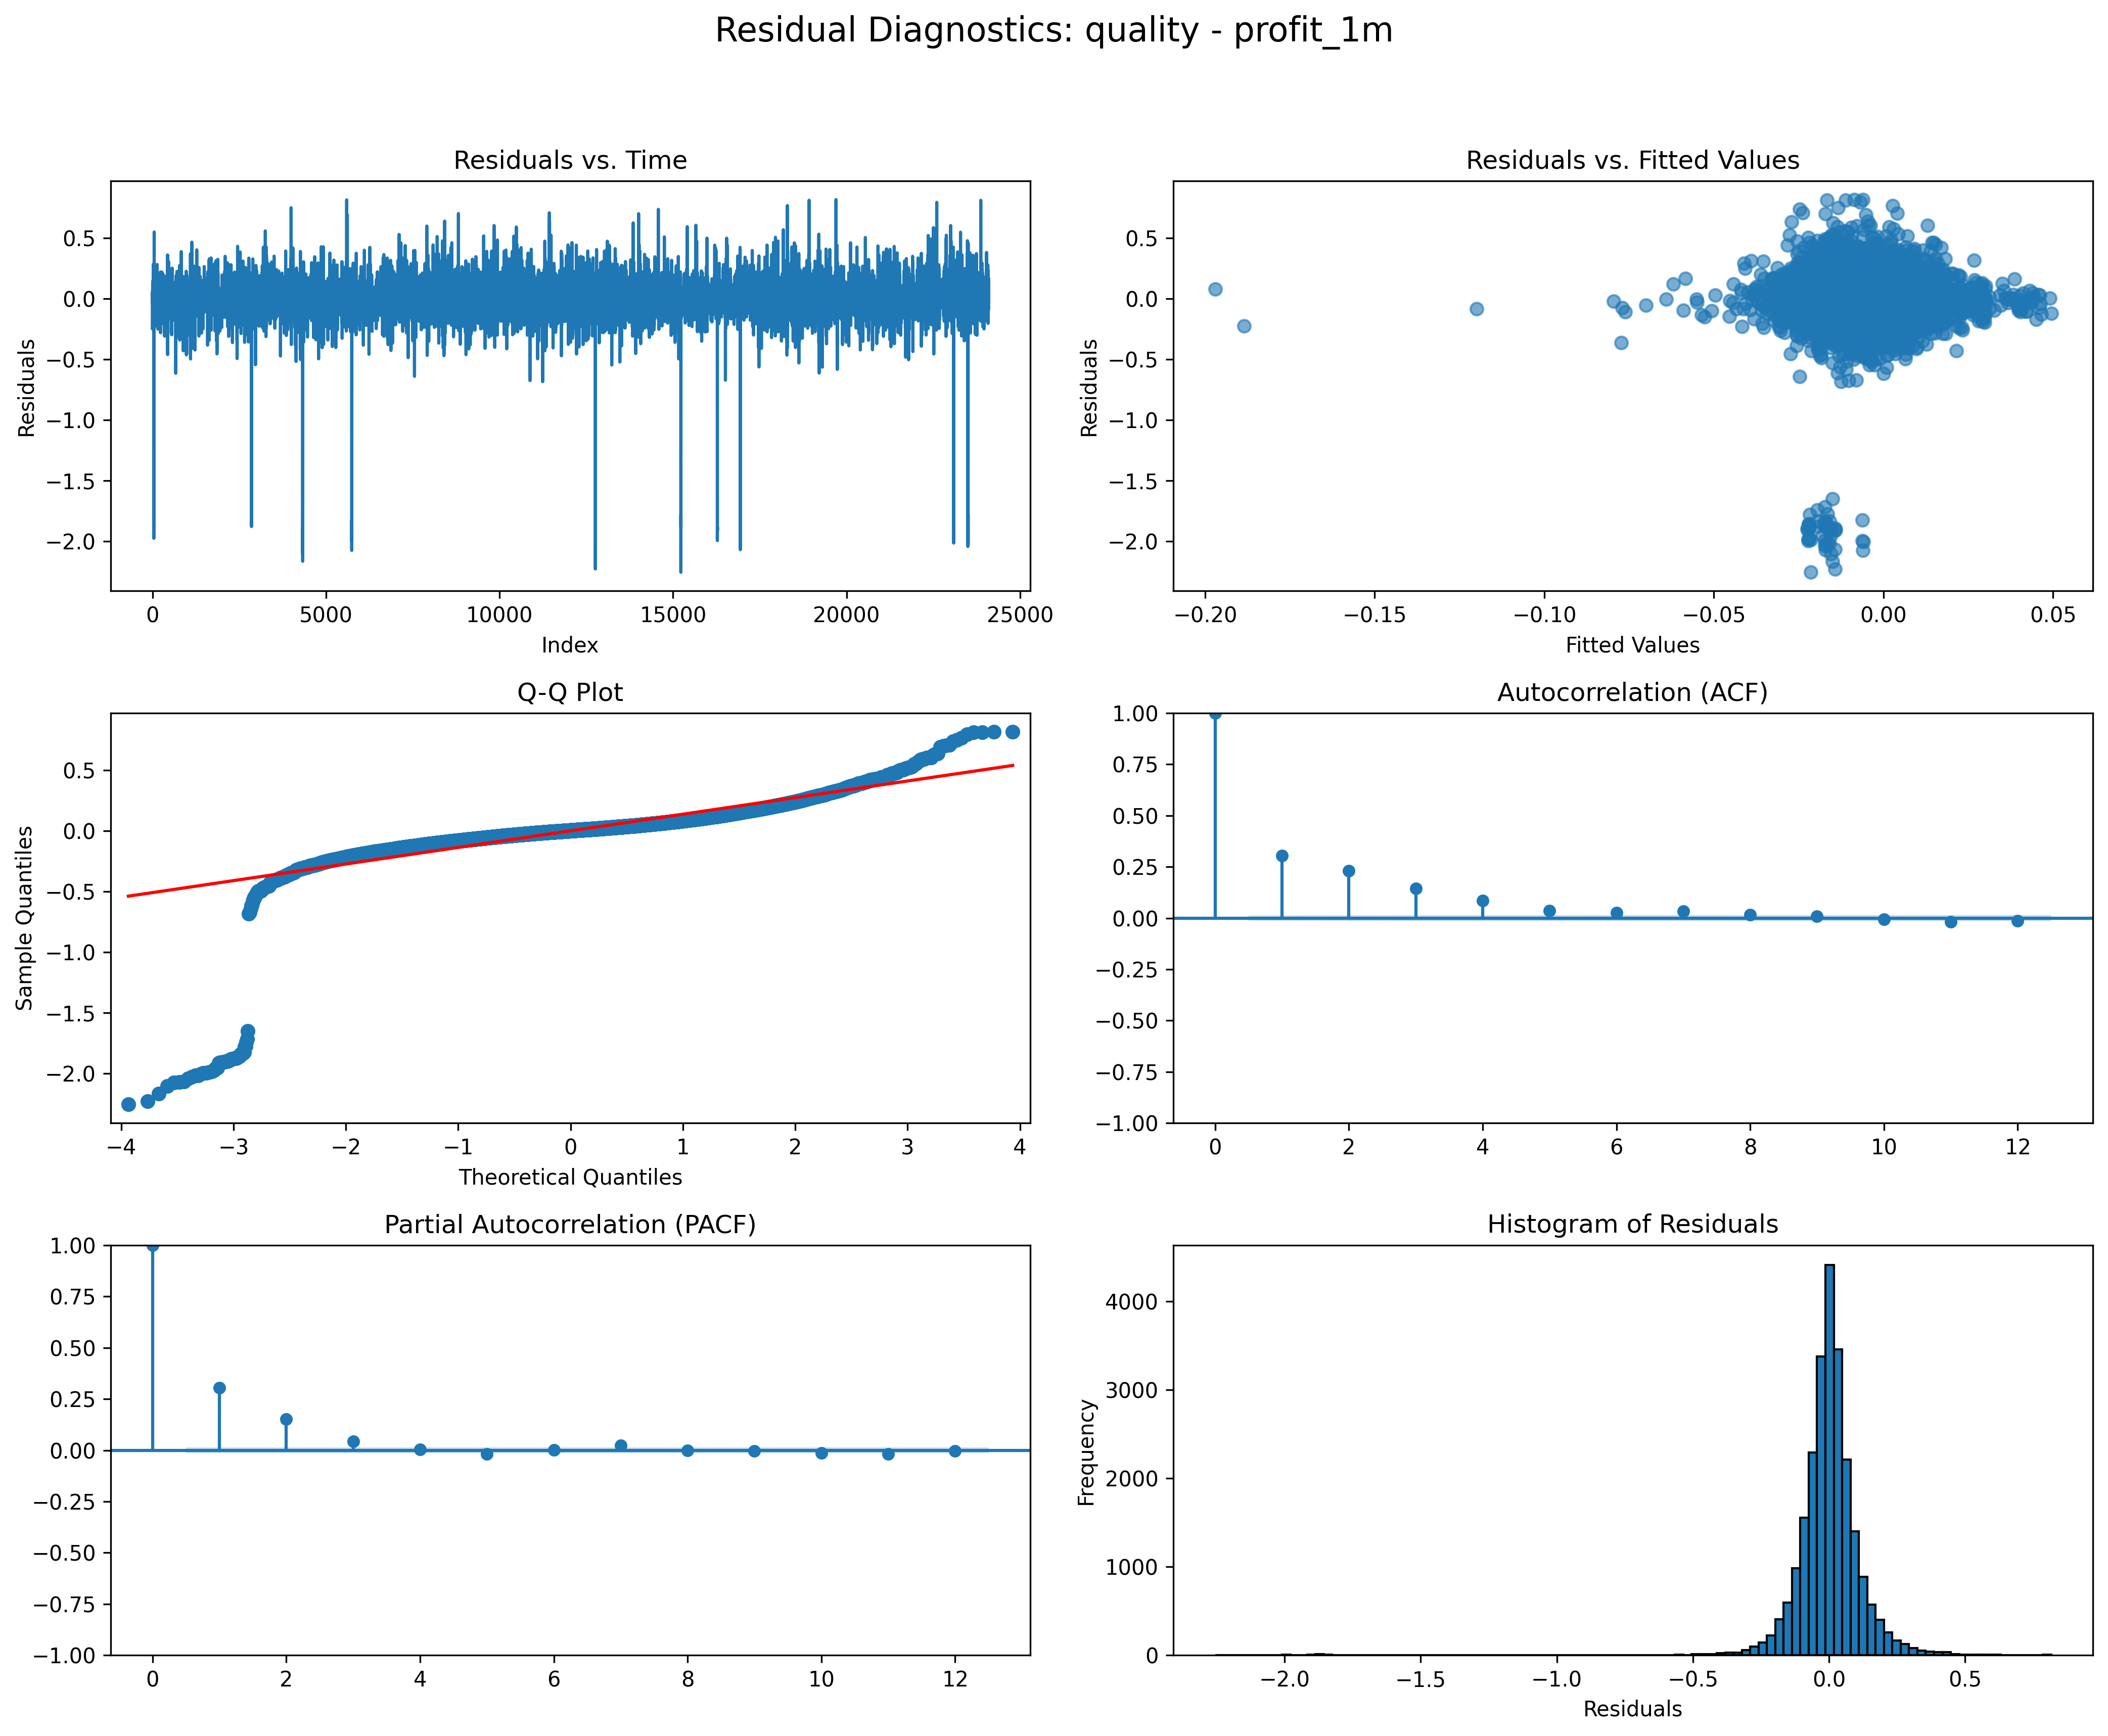
\includegraphics[width=0.32\textwidth]{images/code/models/linear_regression/first_model/Multi/quality_profit_1m_residuals.png}
    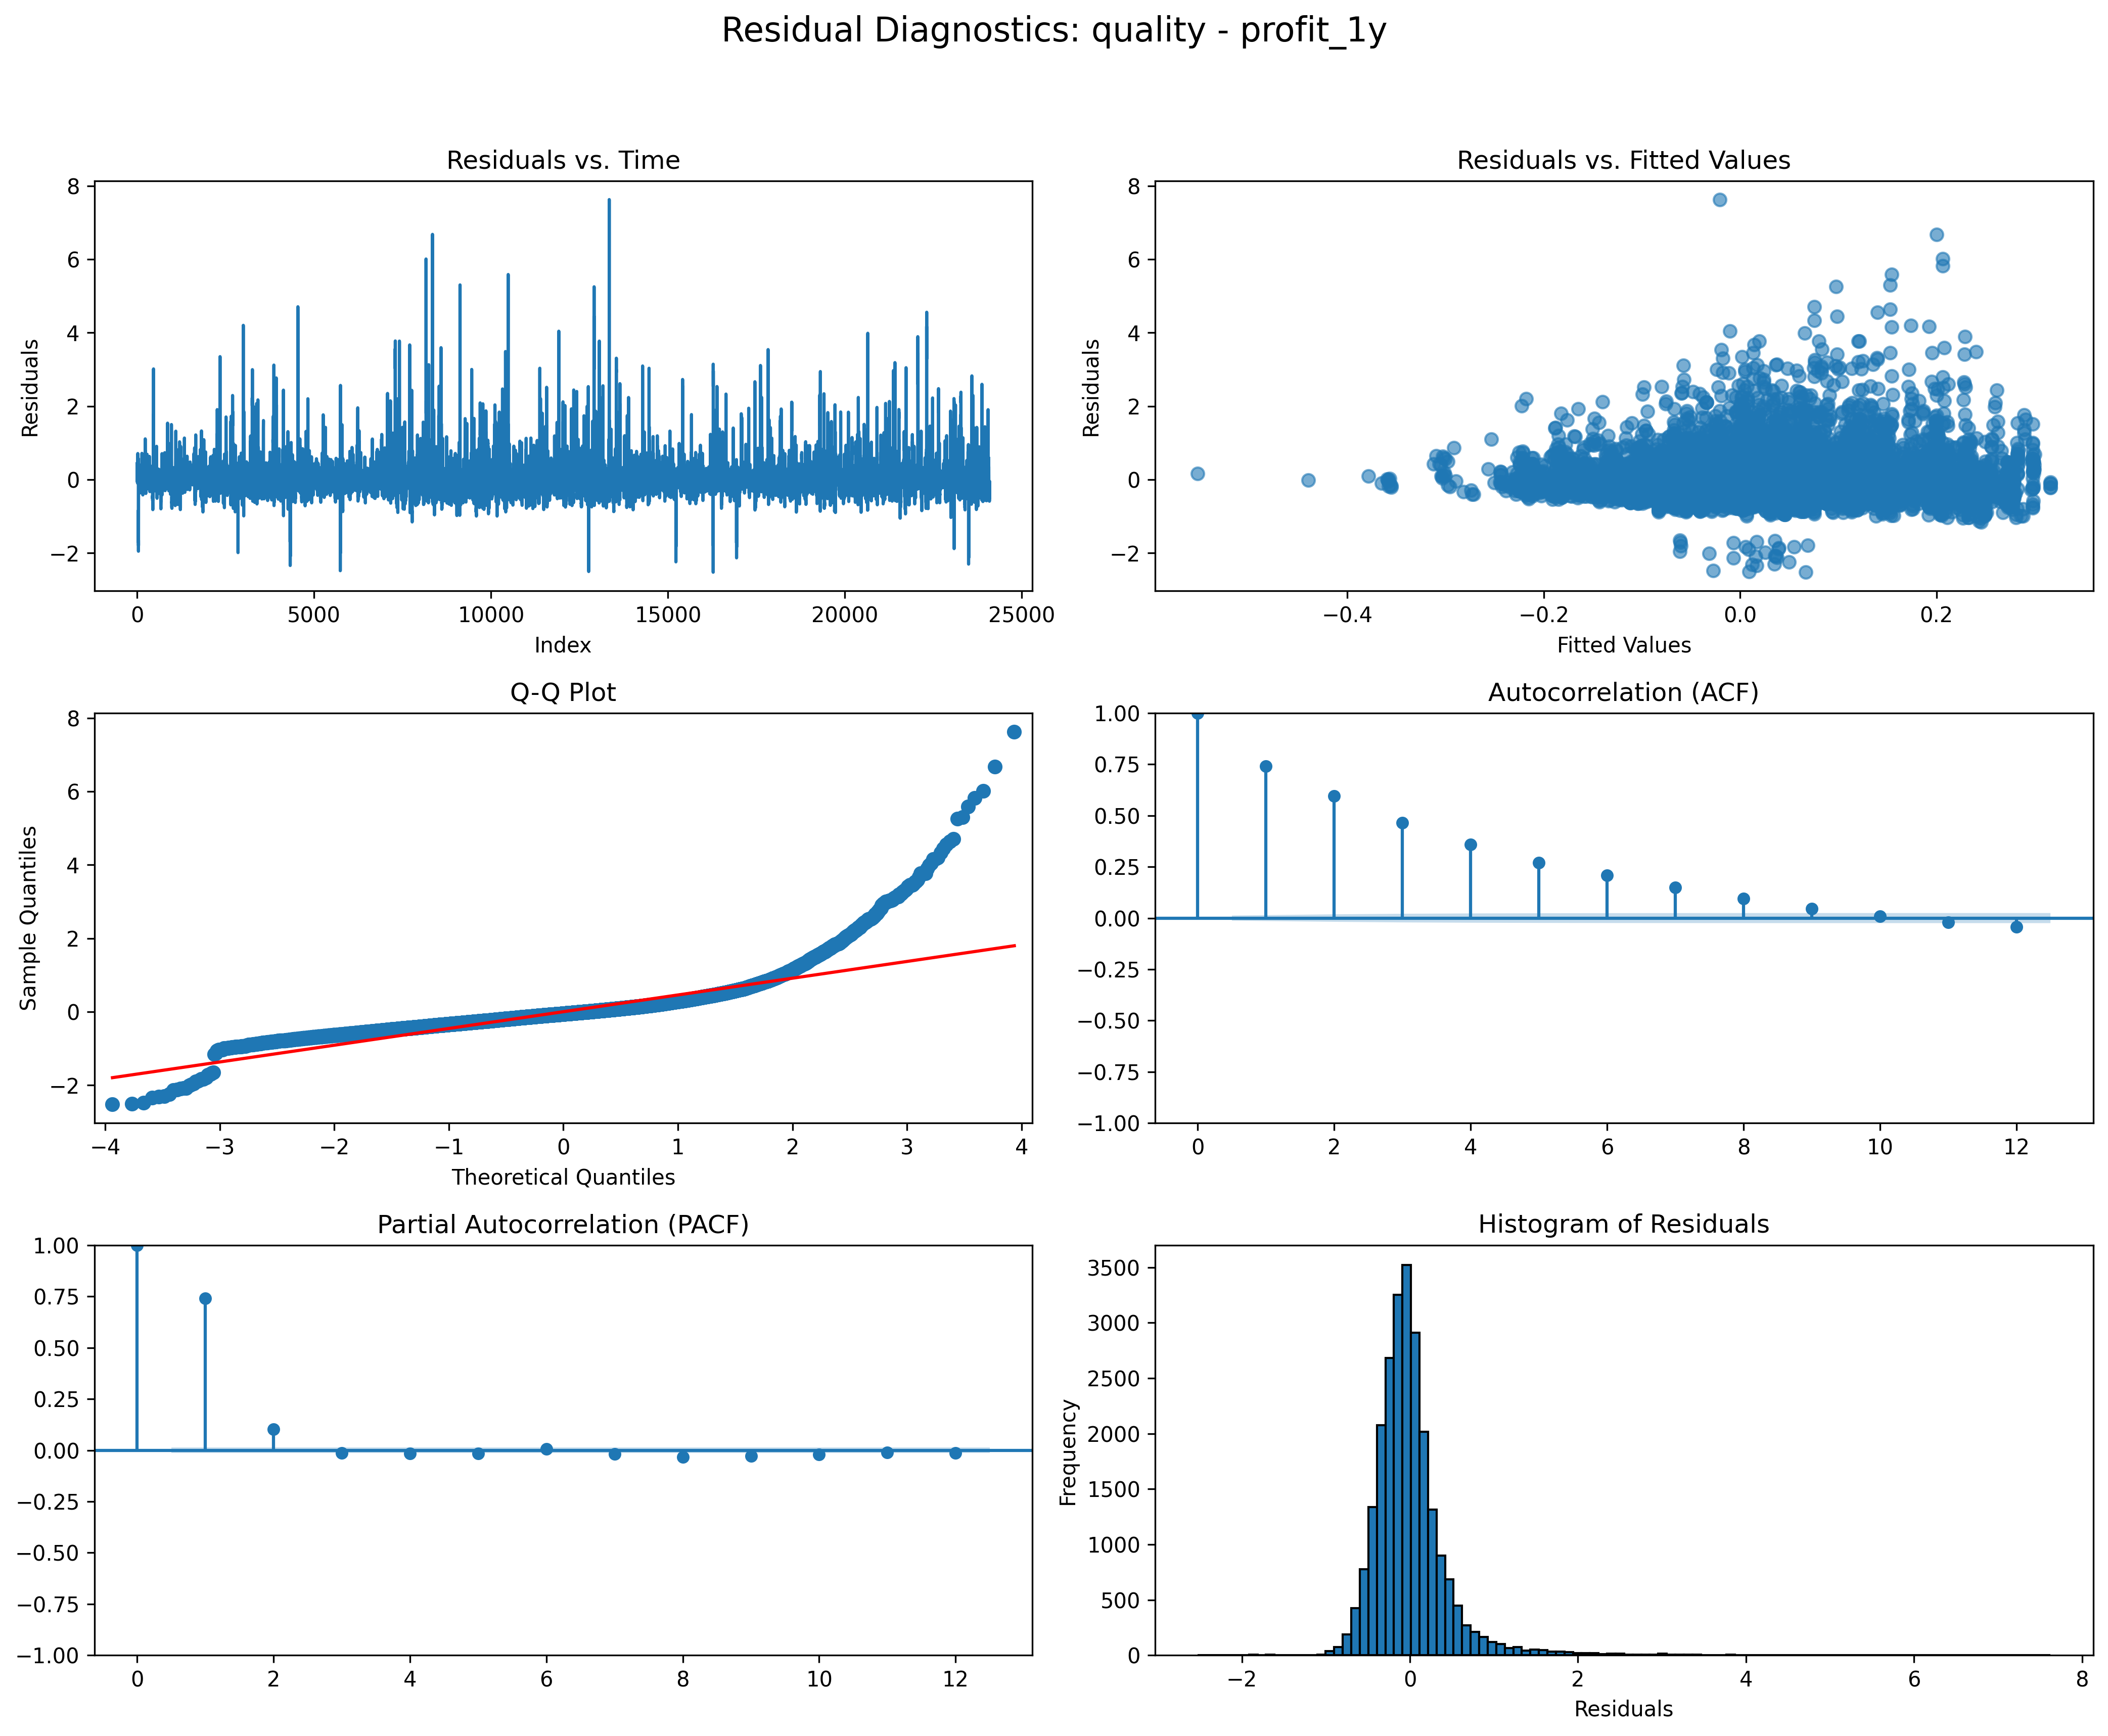
\includegraphics[width=0.32\textwidth]{images/code/models/linear_regression/first_model/Multi/quality_profit_1y_residuals.png}
    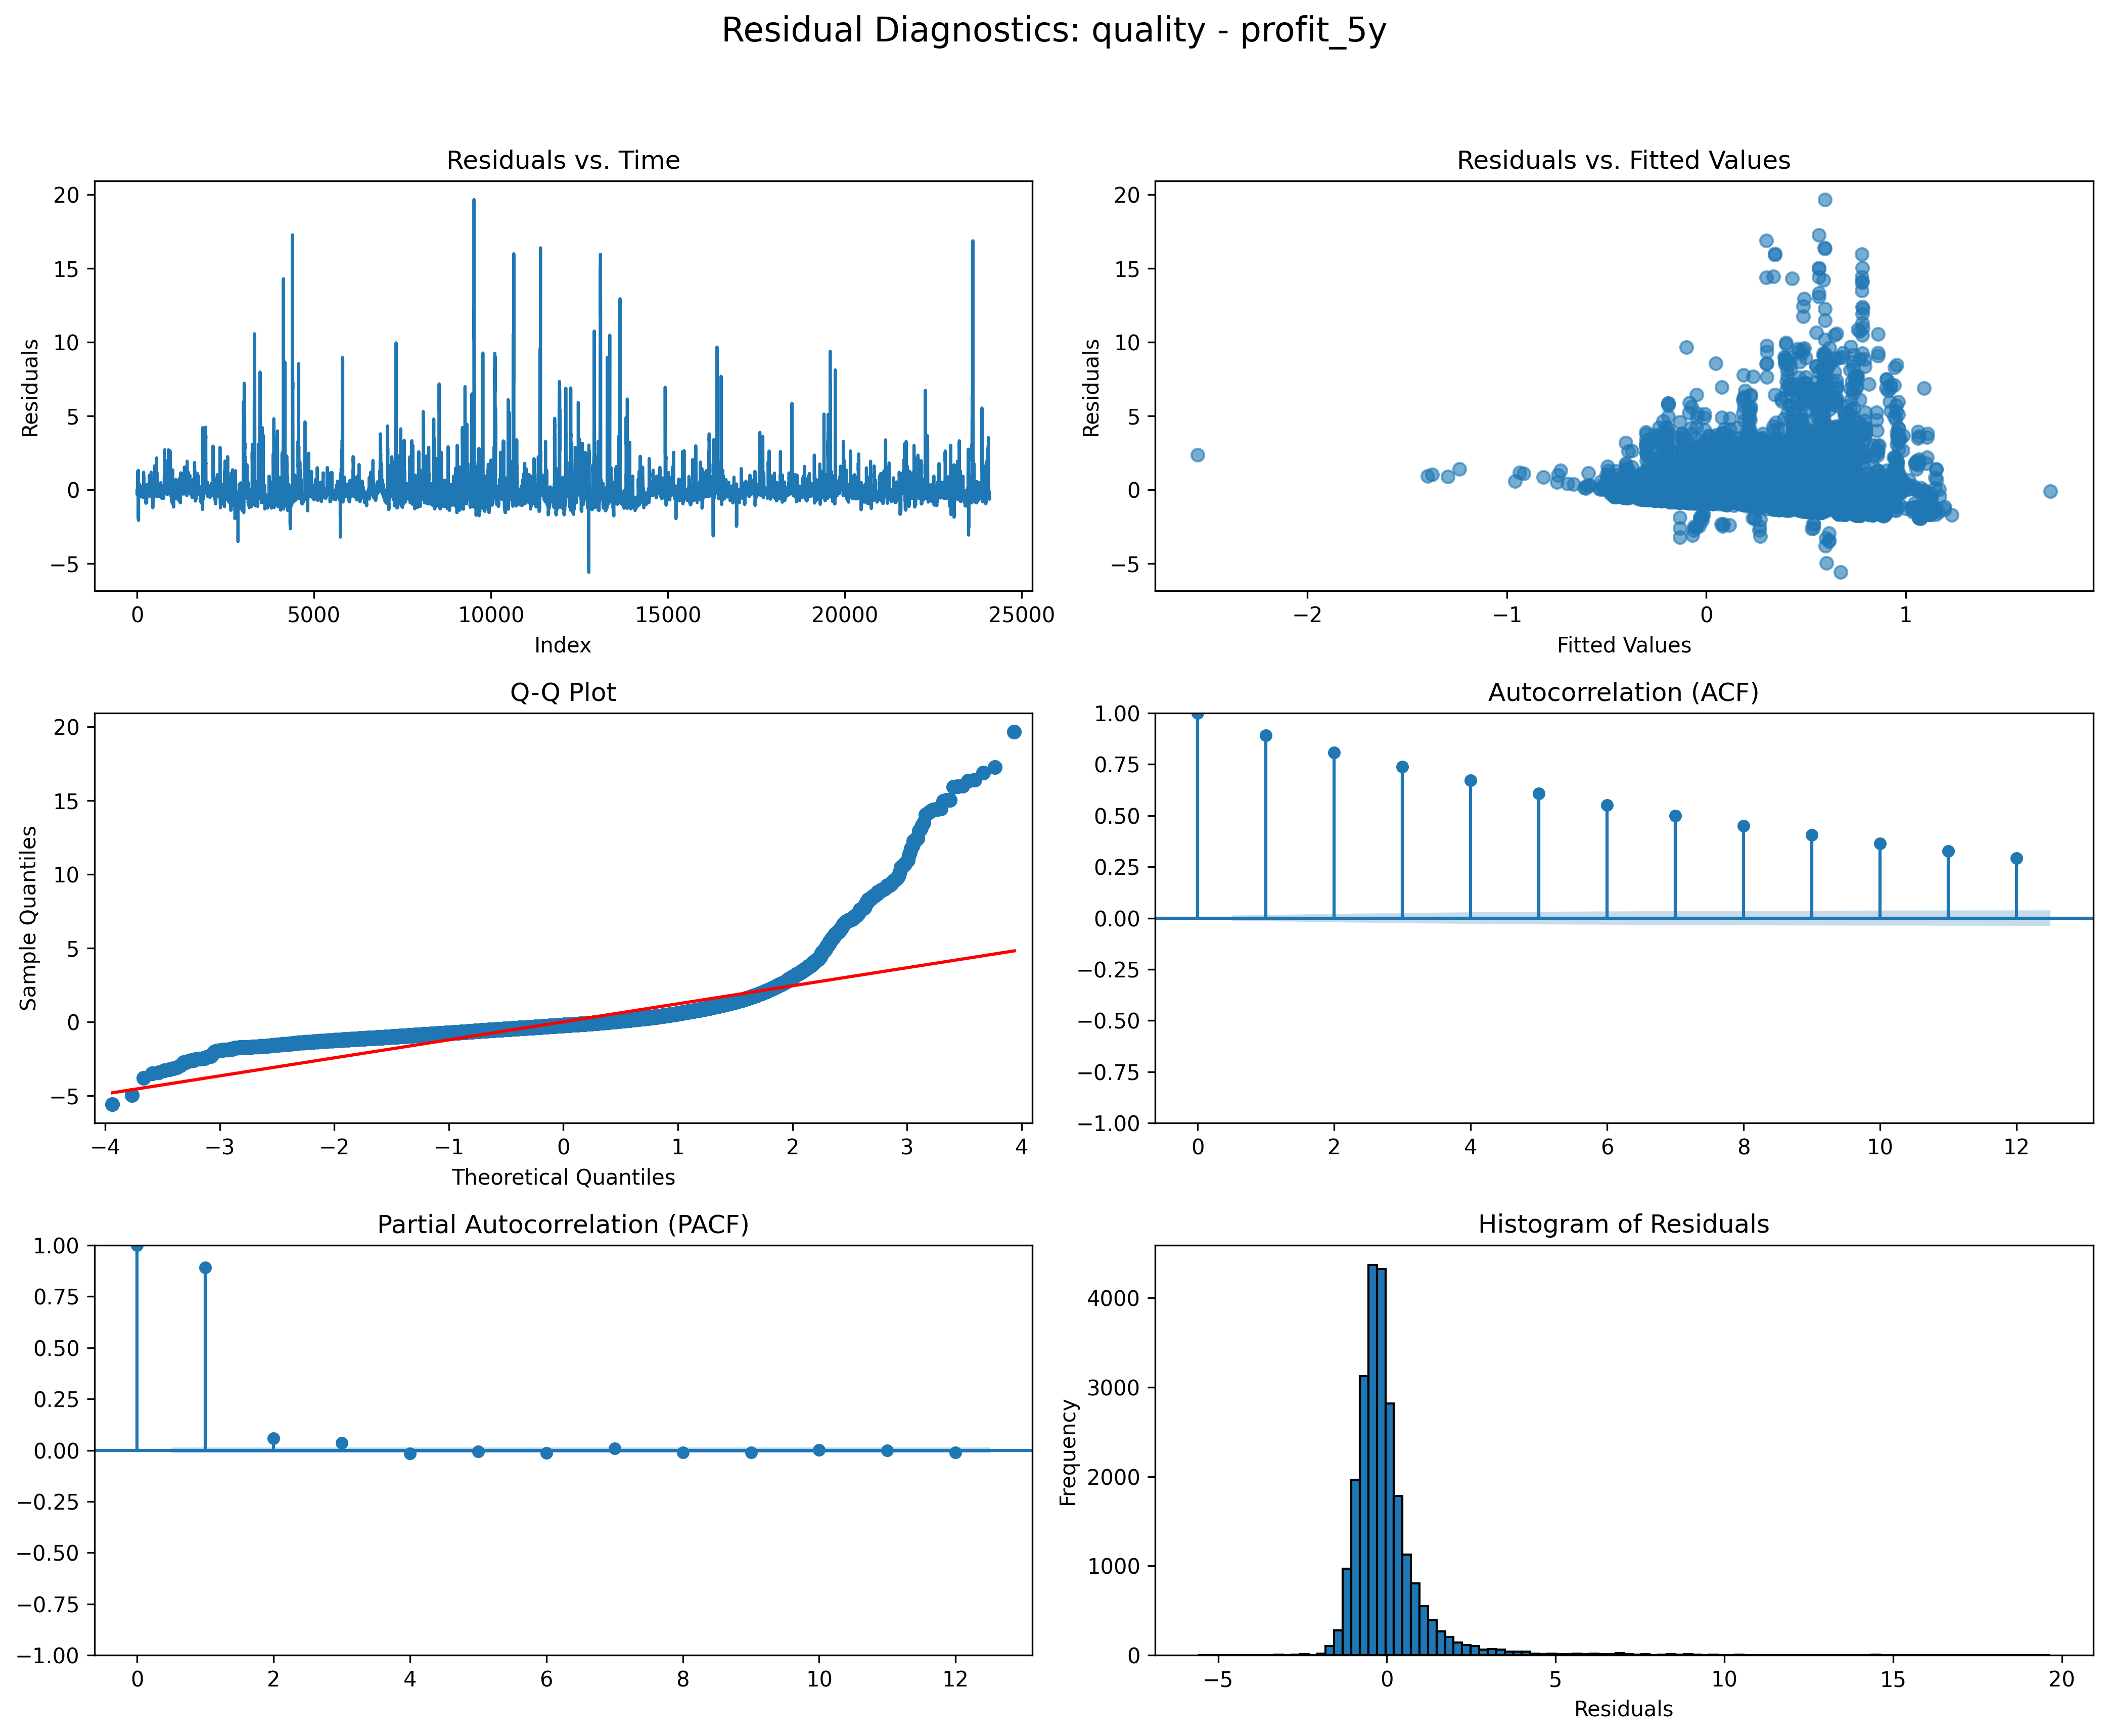
\includegraphics[width=0.32\textwidth]{images/code/models/linear_regression/first_model/Multi/quality_profit_5y_residuals.png}
    \caption{Small Data Future - \acrshort{multi} 5\% - Residuals}
    \label{fig:first_linear_regression_residuals}
\end{figure}

\noindent Examining the residuals, they all show a similar patter that we captured in figure~\ref{fig:first_linear_regression_residuals} with quality for 1m, 1y and 5y profits. We identified several issues:

\begin{itemize}
    \item \textbf{Normality}. The \acrshort{qq} plot reveals that the residuals are not normally distributed, although there is a section where normality appears to hold.
    \item \textbf{Heteroskedasticity}. The residuals vs fitted values plot indicates that the variance is not constant across all time horizons.
    \item \textbf{Autocorrelation}. The \acrshort{acf} and \acrshort{pacf} plots also shows that the residuals are not independent of each other.
    \item \textbf{Outliers}. When looking at the residuals against time, we see big spikes that show that there are many outliers in the data.
\end{itemize}

\noindent Finally we did not even see any consistency with the scores since its effect (sign) kept changing and the coefficients themselves did not have statistical significance.

\begin{table}[H]
    \centering
    \caption{Small Data Future - \acrshort{multi} (4\%) Consistency}
    \begin{tabular}{lccccccc}
        \toprule
        \textbf{Score} & \textbf{Metric} & \textbf{1M} & \textbf{3M} & \textbf{6M} & \textbf{1Y} & \textbf{2Y} & \textbf{5Y} \\
        \midrule
        \multirow{3}{*}{\textbf{Dividend}} 
            & Coef.   & -0.0013 & --      & -0.0004 & -0.0026 & --      & 0.0003 \\
            & Sign    & --      & 0       & --      & --      & 0       & +      \\
            & t-value & -6.38   & --      & -3.22   & -6.92   & --      & 6.44   \\
        \midrule
        \multirow{3}{*}{\textbf{Growth}} 
            & Coef.   & 0.0018  & --      & 0.0007  & 0.0047  & 0.0001  & --     \\
            & Sign    & +       & 0       & +       & +       & +       & 0      \\
            & t-value & 11.27   & --      & 5.75    & 13.86   & 1.62    & --     \\
        \midrule
        \multirow{3}{*}{\textbf{Quality}} 
            & Coef.   & -0.0038 & -0.0059 & -0.0010 & -0.0076 & -0.0003 & 0.0002 \\
            & Sign    & --      & --      & --      & --      & --      & +      \\
            & t-value & -6.93   & -4.54   & -4.29   & -8.61   & -1.87   & 2.47   \\
        \midrule
        \multirow{3}{*}{\textbf{Value}} 
            & Coef.   & 0.0015  & -0.0054 & --      & --      & --      & -0.0002 \\
            & Sign    & +       & --      & 0       & 0       & 0       & --      \\
            & t-value & 4.64    & -4.36   & --      & --      & --      & -1.81   \\
        \bottomrule
    \end{tabular}
    \label{tab:first_linear_regression_results_scores}
\end{table}

\newpage

\subsubsection{The problem with \acrshort{arima}}

\noindent Before jumping into trying to improve the results by refining the data or the models themselves, the first main issue we tried to fix was the autocorrelations seen in the residues. So used an automatic \acrshort{arima} fitter from \textit{PyPI} \textcite{pmdarima2025} to see if it improved the performance of the linear regression models and also fix the issue all together.

\begin{figure}[H]
    \centering
    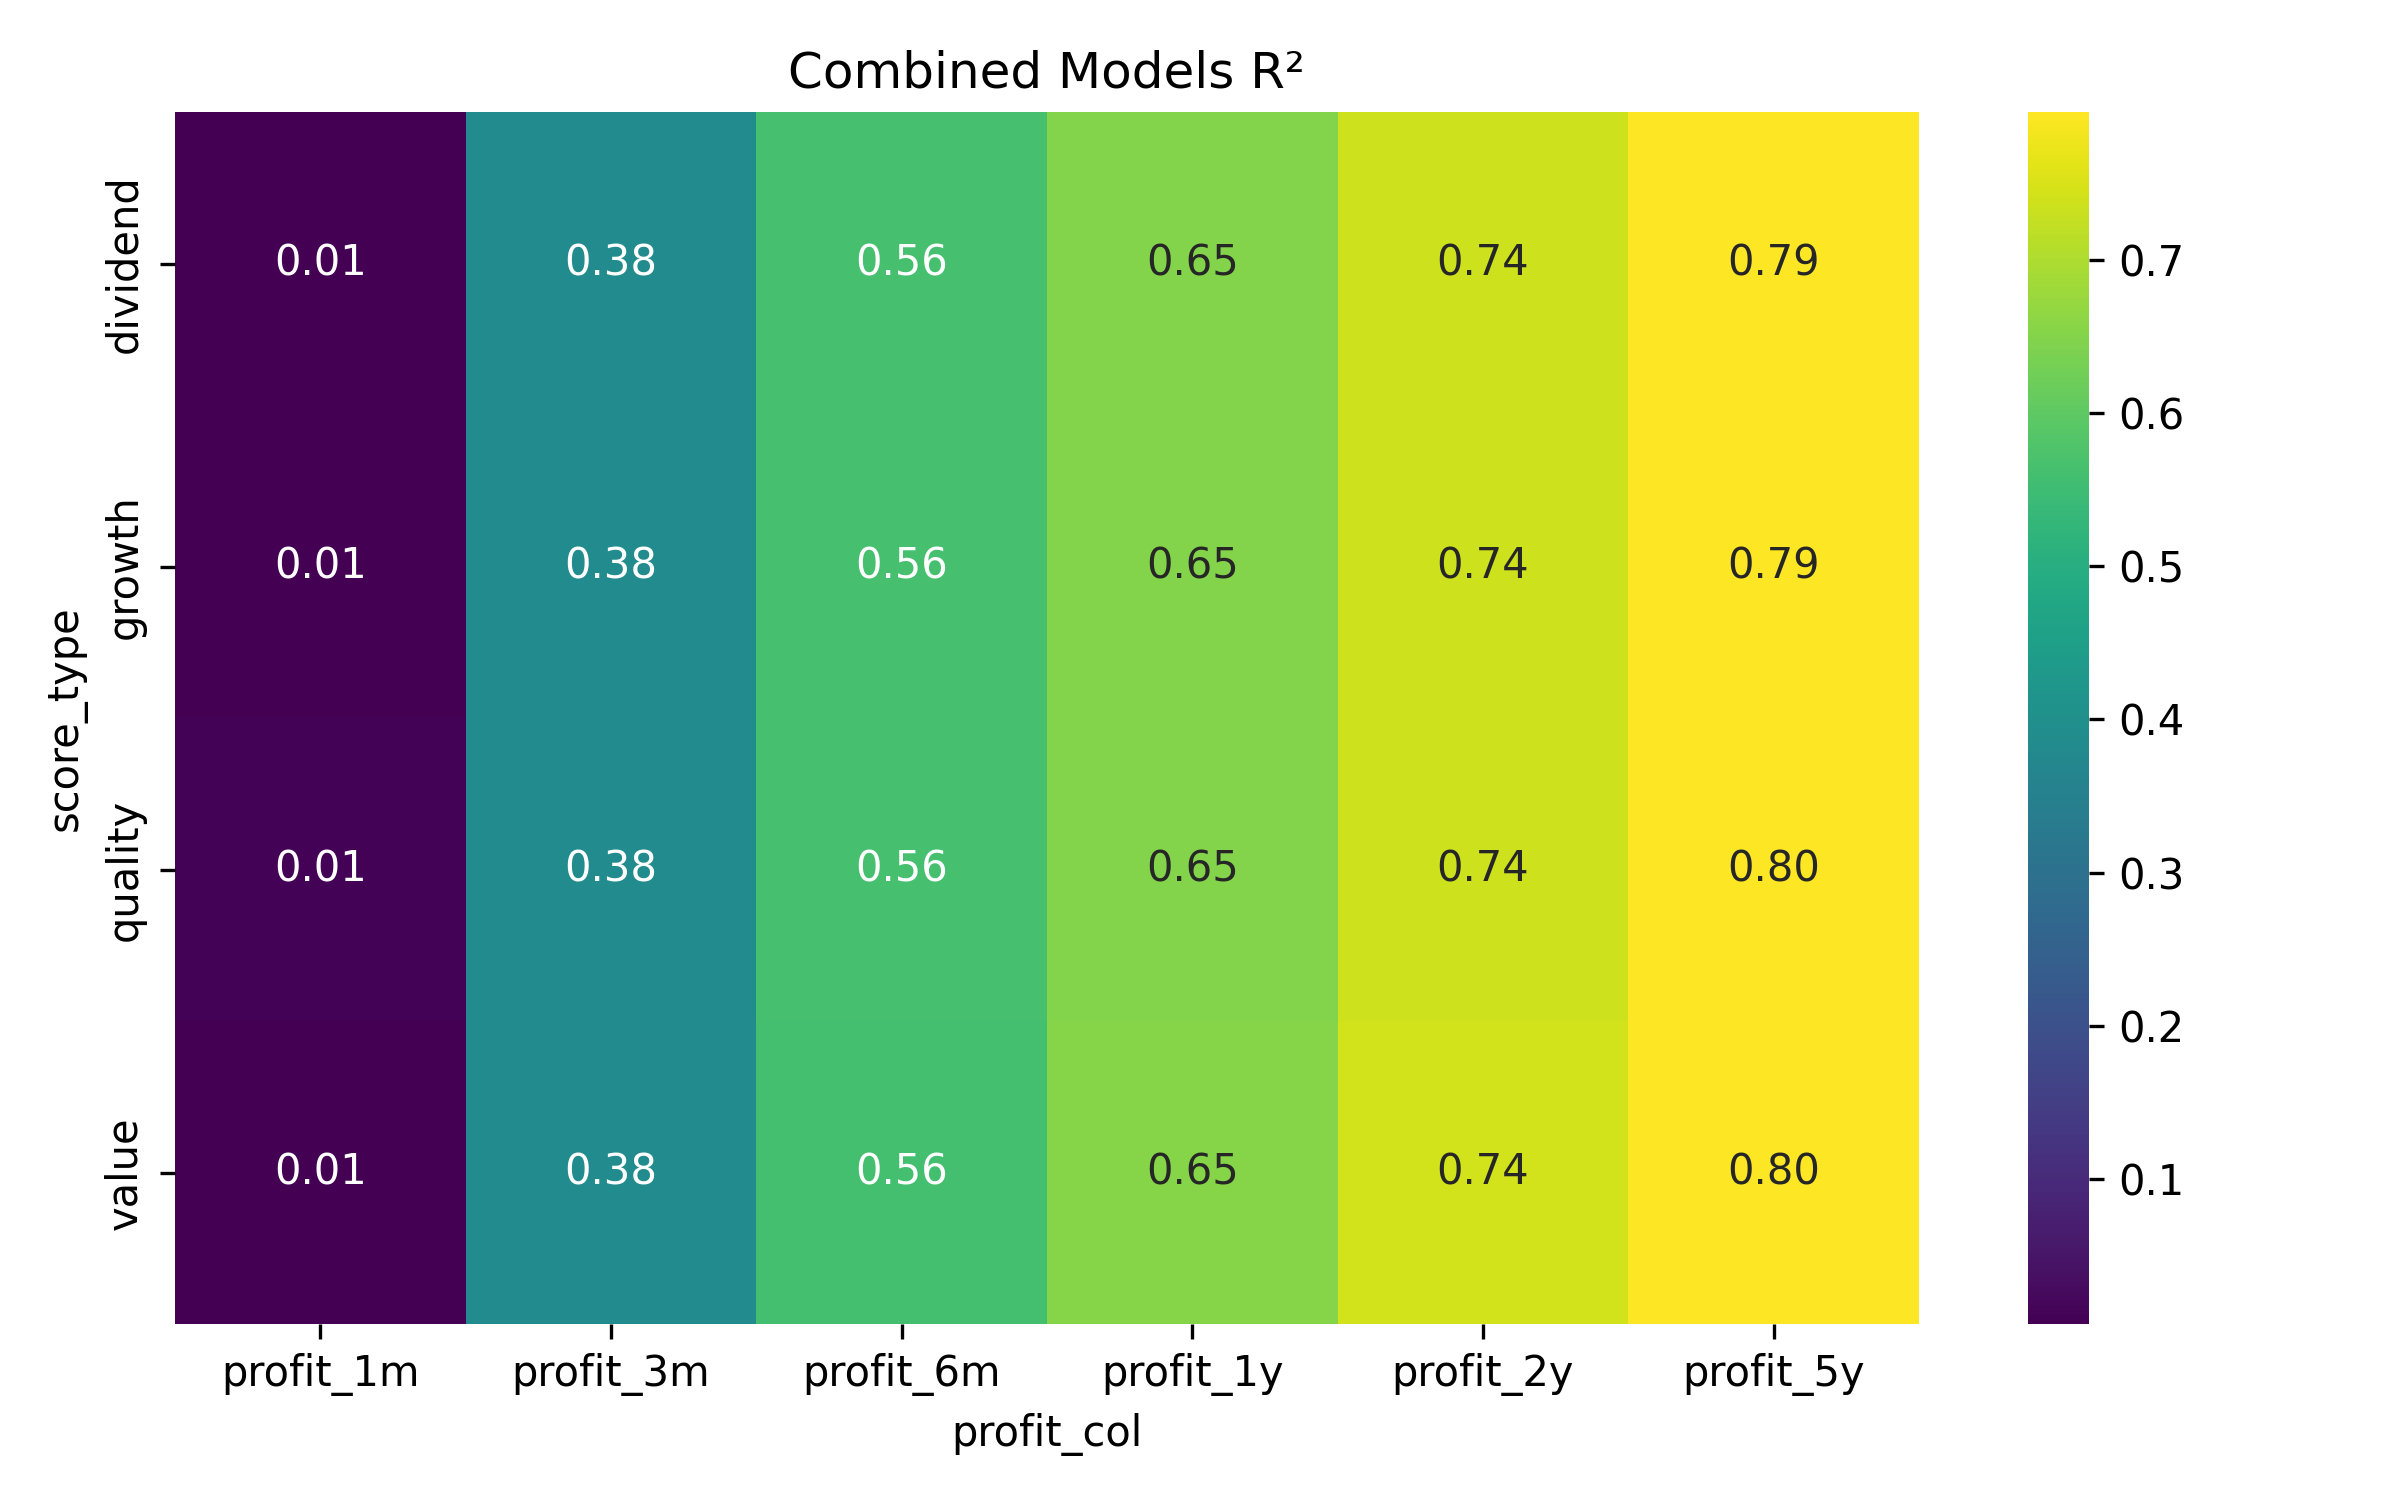
\includegraphics[width=1\textwidth]{images/code/models/linear_regression/ARIMA_performance.png}
    \caption{Small Data Future - \acrshort{multi} (4\%)}
    \label{fig:arima_linear_regression}
\end{figure}

\noindent And of course, this worked amazingly: it solved completely the autocorrelations of the residues and it improved a lot the performance of the model (figure~\ref{fig:arima_linear_regression}). But this came with a major issue that made us abandon the idea of using \acrshort{arima} models; \textbf{we had to use future profits as inputs for the \acrshort{arima} model}, which only could make sense for an ad-hoc model to explain past behavior, but not for a model that is supposed to predict future behavior.

\subsubsection{Artificial Normality}

\noindent So before continuing with the autocorrelations issue, we tried to solve the normality and heteroskedasticity issues. And since it is well known that regression models are not very robust to non-normal data fixing these should also improve the models' performance. We used the mentioned \textit{Yeo-Johnson} transformation and saw some \textbf{improvements with the performances and the \acrshort{rmse} for long term models (5y)} but showed complete noise for the short term (1m to 6m), which suggest that this transformation helped coping with the tails of the 5y-profits distribution and also helped showing the real noise from the short term models. In general, we see a \textbf{worsening of the accuracy} in most of the models, except in the long term.

\begin{figure}[H]
    \centering
    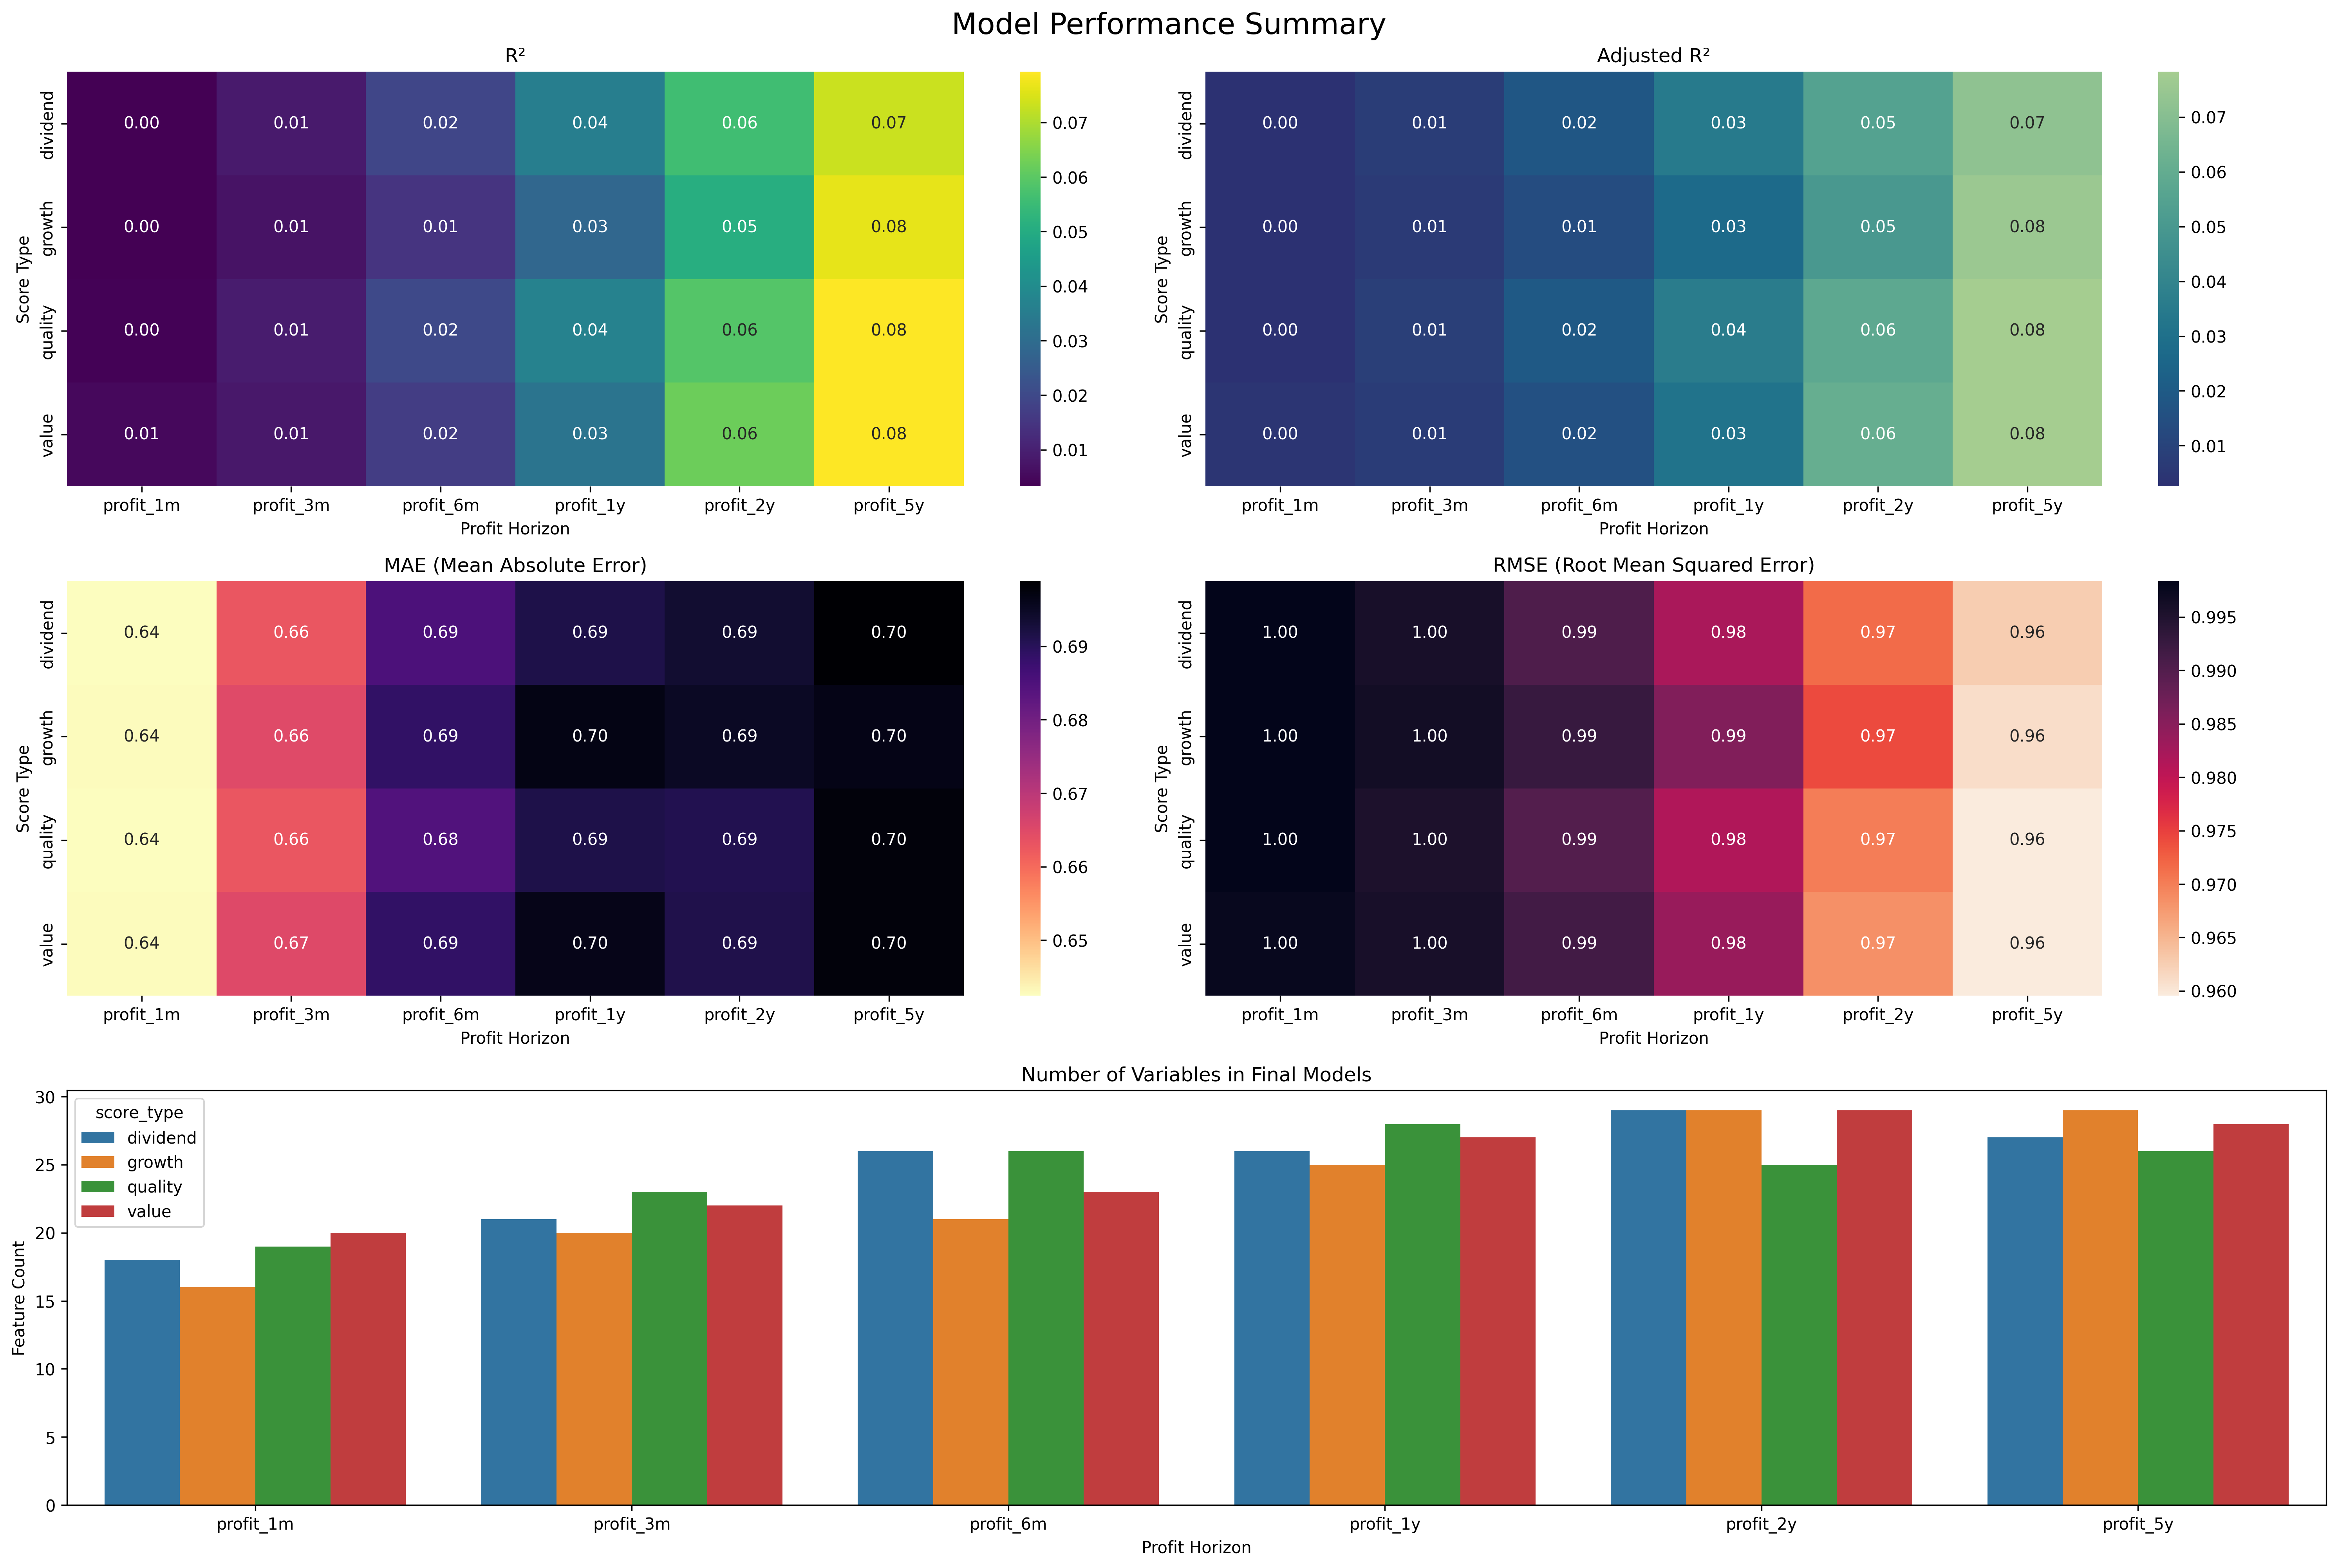
\includegraphics[width=1\textwidth]{images/code/models/linear_regression/first_model/Small Data future - Multi Gaussian performance.png}
    \caption{Small Data Future \textit{Yeo-Johnson} - \acrshort{multi} (4\%)}
    \label{fig:first_linear_regression_gaussian}
\end{figure}

\noindent When looking at the residuals in figure~\ref{fig:first_linear_regression_gaussian_residuals}, we can see that the \textbf{normality had improved a lot} for the mid and long term models --which aligns with the accuracies changes--, but we still have issues in the tails of the \acrshort{qq} plot and the same peaks in the time series plots.

\begin{figure}[H]
    \centering
    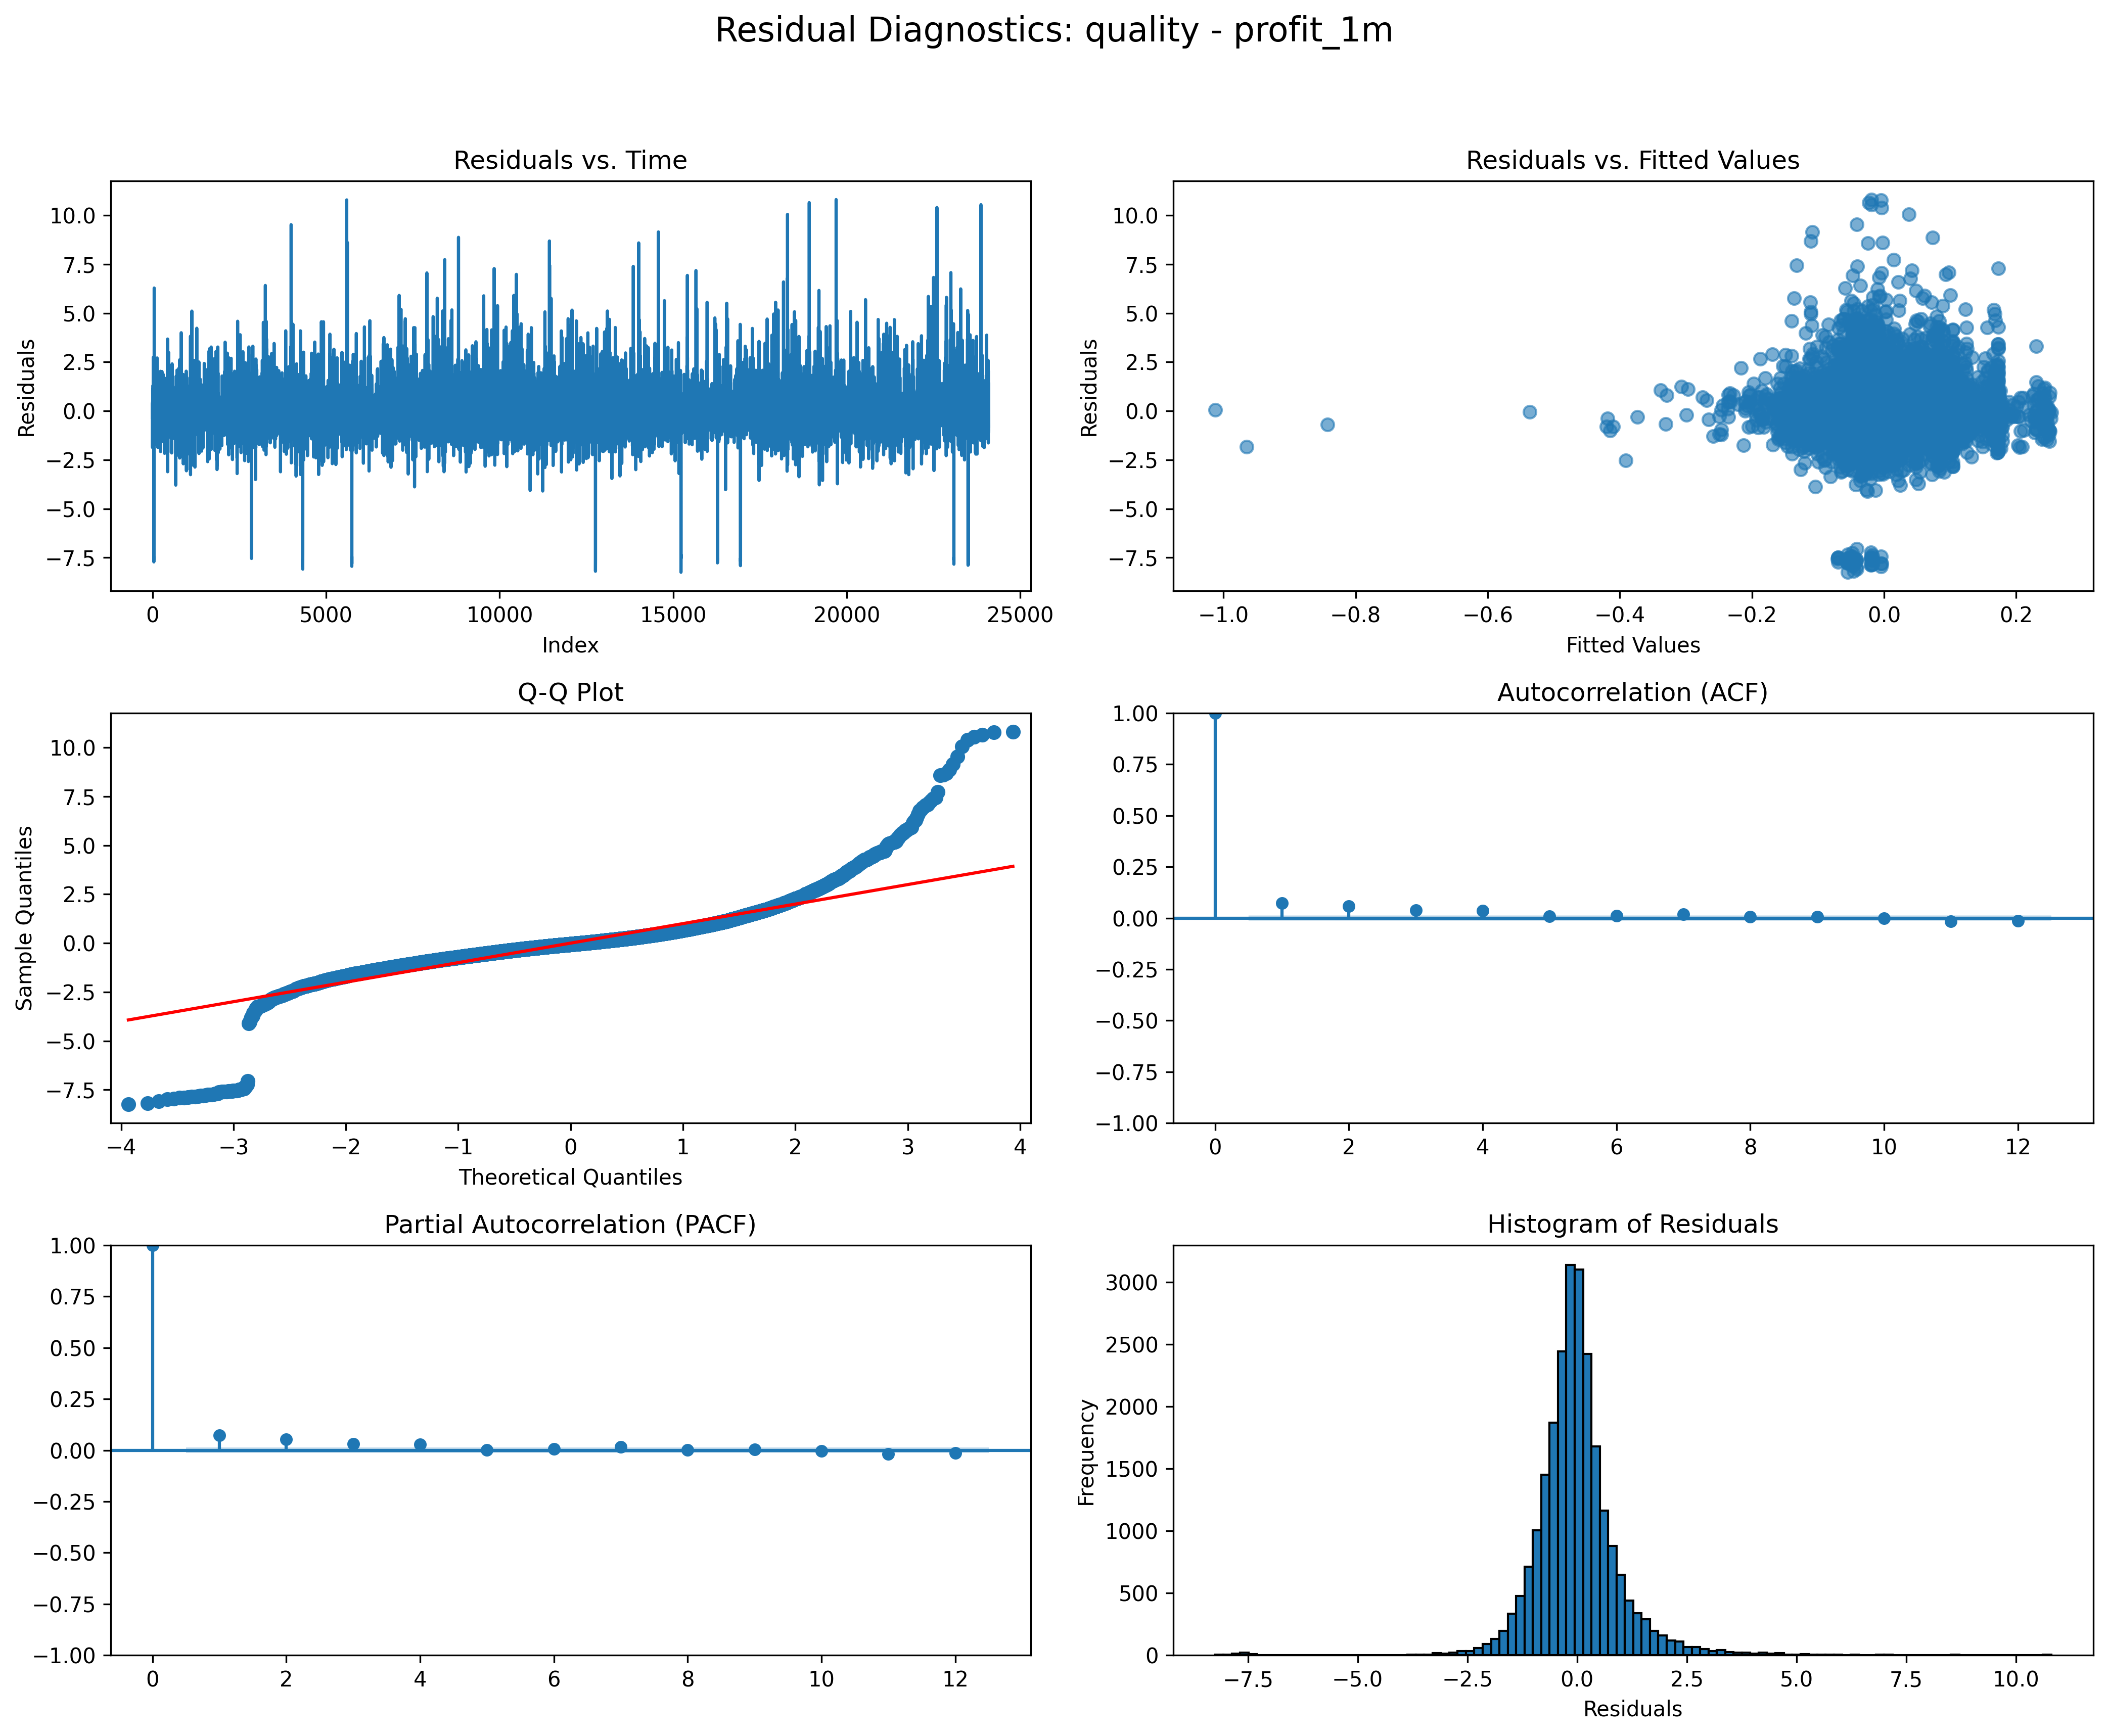
\includegraphics[width=0.32\textwidth]{images/code/models/linear_regression/first_model/Multi/quality_profit_1m_residuals - Gaussian.png}
    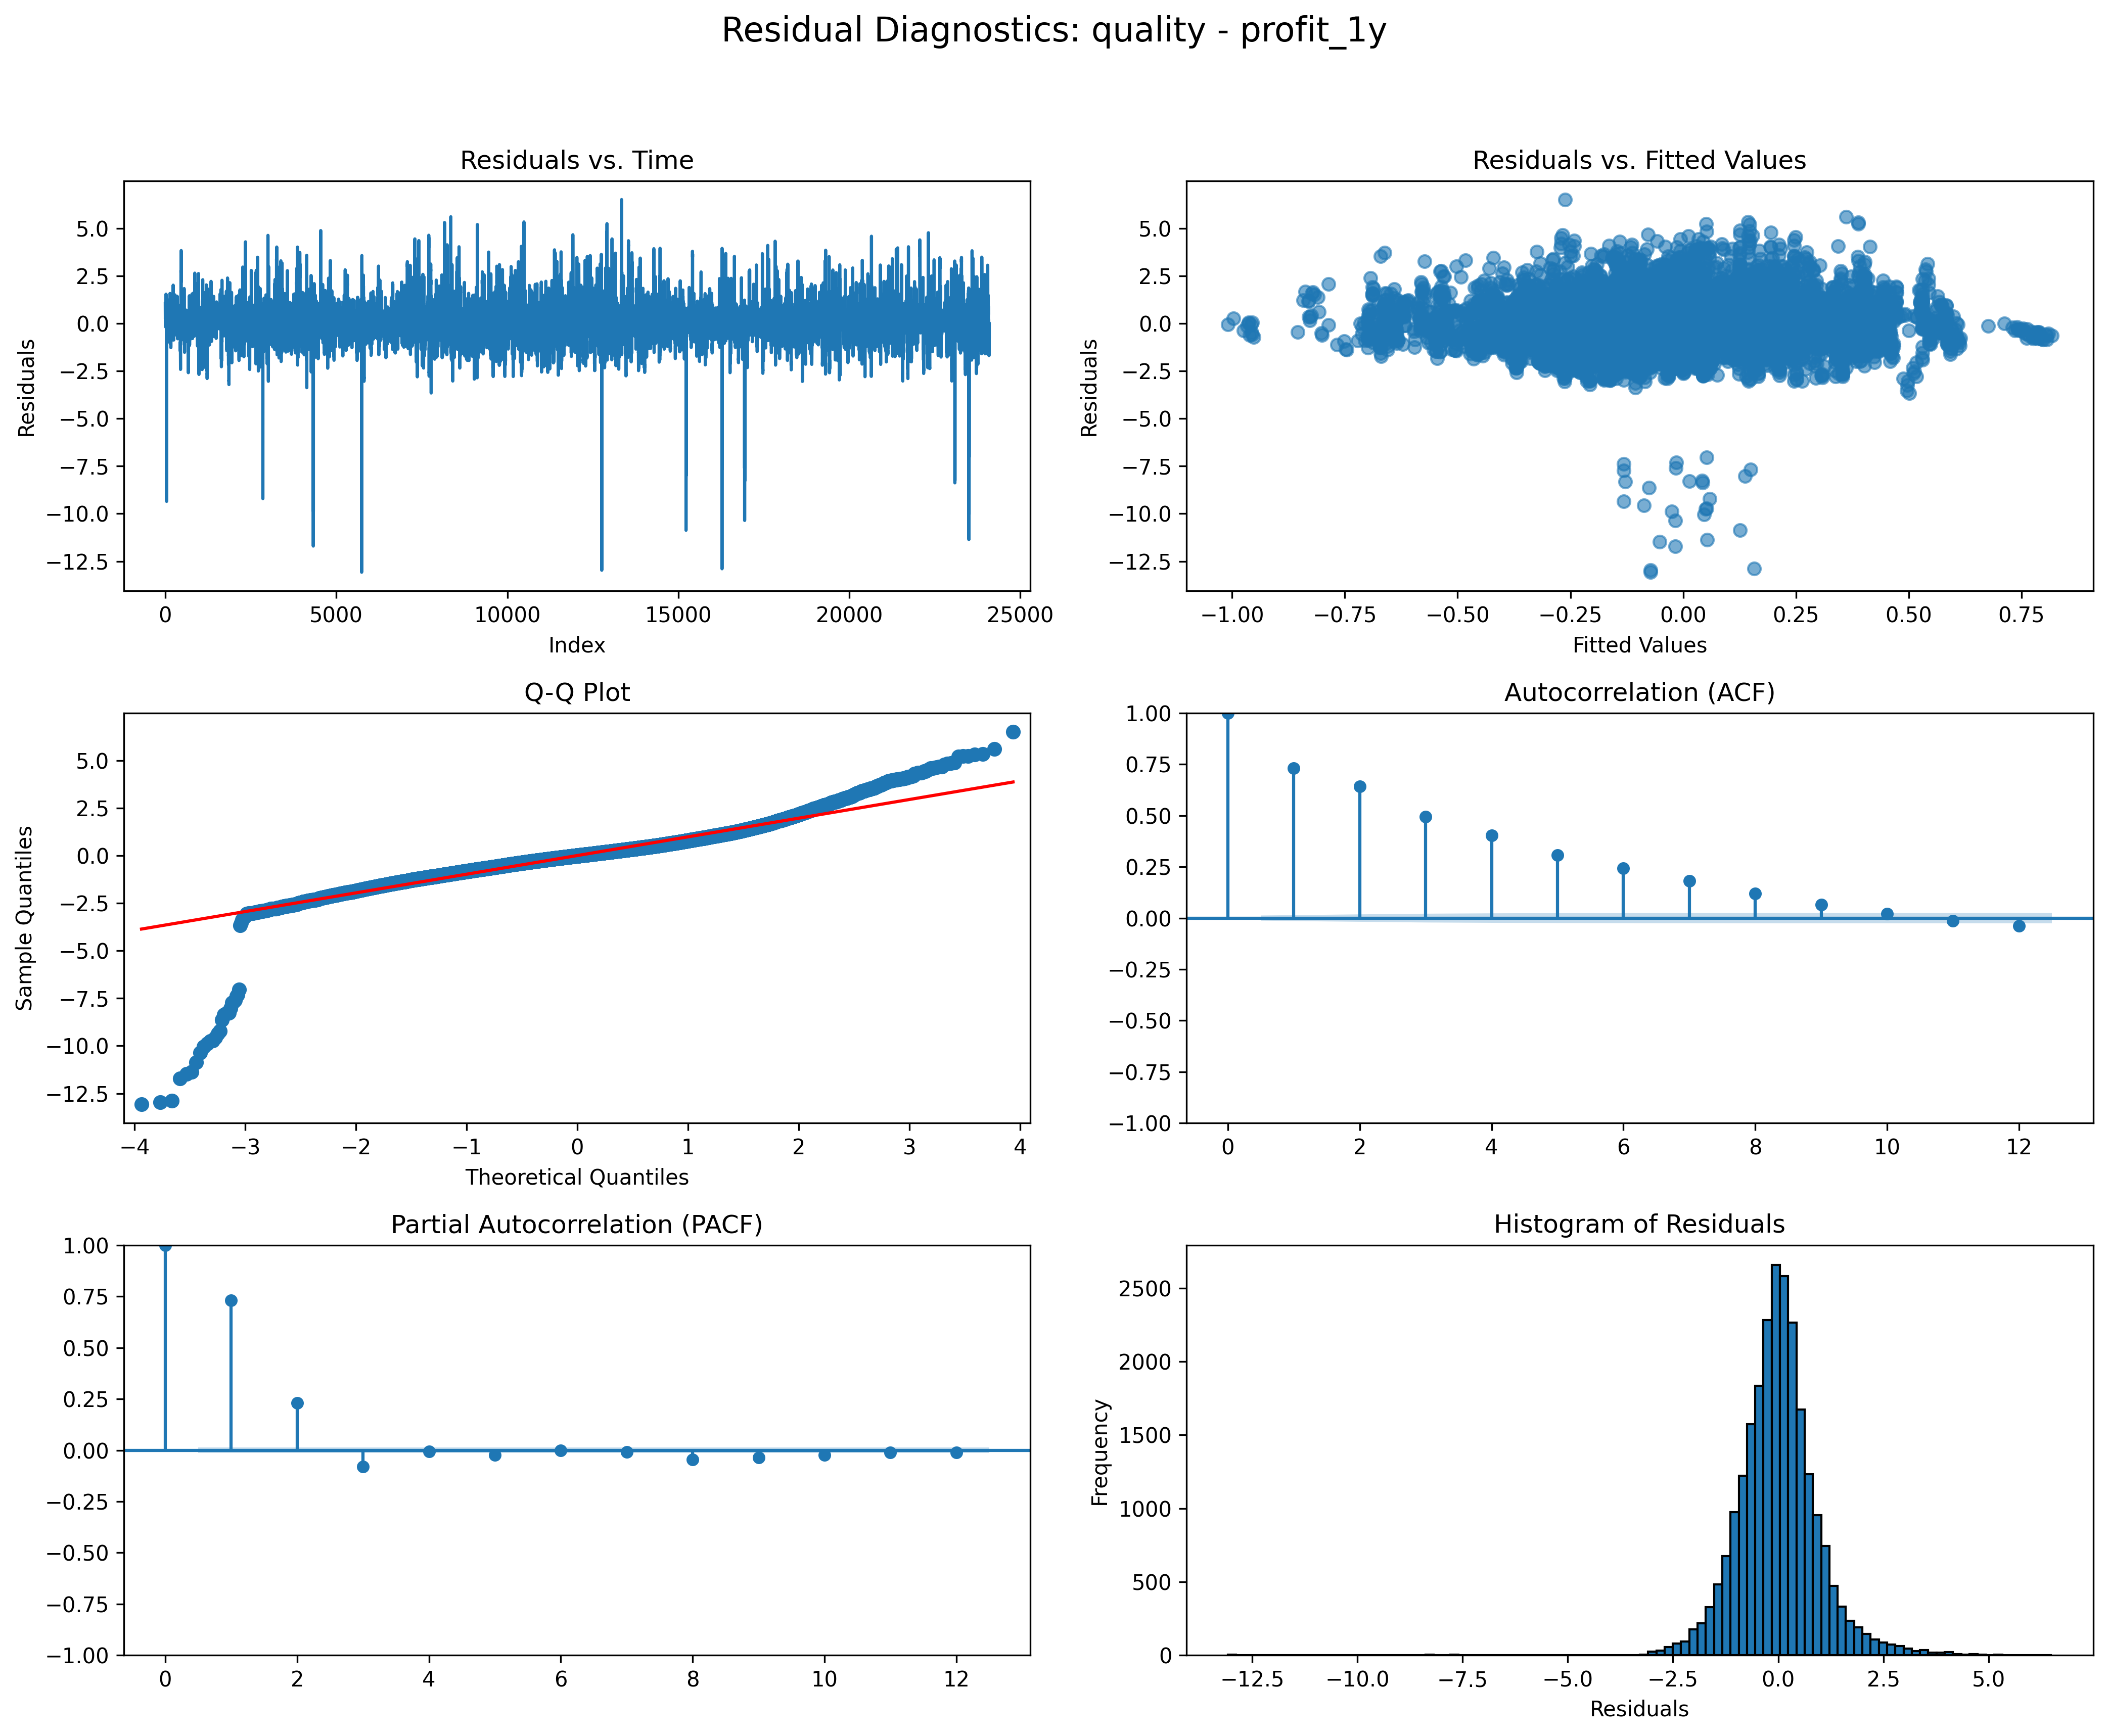
\includegraphics[width=0.32\textwidth]{images/code/models/linear_regression/first_model/Multi/quality_profit_1y_residuals - Gaussian.png}
    \includegraphics[width=0.32\textwidth]{images/code/models/linear_regression/first_model/Multi/quality_profit_5y_residuals - Gaussian.png}
    \caption{Small Data Future \textit{Yeo-Johnson} - \acrshort{multi} (4\%)}
    \label{fig:first_linear_regression_gaussian_residuals}
\end{figure}

\noindent Also, after this transformation we still didn't see any consistency and statistical significance (see appendix Table~\ref{tab:first_linear_regression_results_scores_gaussian}). But since it improved both the performance and the normality \textbf{we applied this transformation for the rest of the models}.

\subsubsection{Windowed Models}

\noindent Before seeing if the regions' non-linear effects were causing the some of issues, we wanted to try to improve the autocorrelations by using a different approach. In this case, we used a new family of windowed models with the different statistics explained to see if the market had any memory with past financial performances.

\begin{figure}[H]
    \centering
    \includegraphics[width=1\textwidth]{images/code/models/linear_regression/third_model/Small Data future - Multi performance.png}
    \caption{Small Data Future (Windowed) - \acrshort{multi} (4\%)}
    \label{fig:third_linear_regression_summary}
\end{figure}

\noindent In figure~\ref{fig:third_linear_regression_summary} it appears to be a general improvement into all of the models' performance and accuracy, but this could be due to the increase of explanatory variables --overfitting--. But we encounter a new patter that will be happening in all of the models that uses these windows: \textbf{increase in the Value's models performance and accuracy, with a peak around 6m-profits}. To understand this, we have to go back to the definition of the Value Score seen in chapter 2, where it was clear that the score contains the price movements within it. So we have figured out a way to implement some of the price's momentum into the models including also financial data into it. This showed us that \textbf{the market has memory of a company's price multiples}.

\begin{figure}[H]
    \centering
    \includegraphics[width=0.32\textwidth]{images/code/models/linear_regression/third_model/Multi/quality_profit_1m_residuals.png}
    \includegraphics[width=0.32\textwidth]{images/code/models/linear_regression/third_model/Multi/quality_profit_1y_residuals.png}
    \includegraphics[width=0.32\textwidth]{images/code/models/linear_regression/third_model/Multi/quality_profit_5y_residuals.png}
    \caption{Small Data Future (Windowed) - \acrshort{multi} (4\%)}
    \label{fig:third_linear_regression_residuals}
\end{figure}

\noindent The residues kept having the same issues as the previous models, but we finally see \textbf{consistency and significance}. In Table~\ref{tab:third_linear_regression_results_scores} we made a summary of the only relevant results, but for the full data see appendix Tables 6.2--6.5.

\begin{table}[H]
    \centering
    \caption{Small Data Future (Windowed) - \acrshort{multi} (4\%) Consistency Summary}
    \begin{tabular}{lccccccc}
        \toprule
        \textbf{Score} & \textbf{Metric} & \textbf{1M} & \textbf{3M} & \textbf{6M} & \textbf{1Y} & \textbf{2Y} & \textbf{5Y} \\
        \midrule
        \multirow{3}{*}{\textbf{Dividend\_24m\_avg}} 
        & Coef.   & 0.0041   & 0.0073  & 0.0154  & 0.0172  & 0.0268  & 0.0328  \\
        & \textbf{\textcolor{green}{Sign}}
                     & \textbf{\textcolor{green}{+}}
                     & \textbf{\textcolor{green}{+}}
                     & \textbf{\textcolor{green}{+}}
                     & \textbf{\textcolor{green}{+}}
                     & \textbf{\textcolor{green}{+}}
                     & \textbf{\textcolor{green}{+}} \\
        & \textbf{\textcolor{green}{t-value}}
                     & \textbf{\textcolor{green}{5.09}}
                     & \textbf{\textcolor{green}{6.97}}
                     & \textbf{\textcolor{green}{7.27}}
                     & \textbf{\textcolor{green}{13.30}}
                     & \textbf{\textcolor{green}{13.01}}
                     & \textbf{\textcolor{green}{11.94}} \\
        \midrule
        \multirow{3}{*}{\textbf{Growth\_12m\_avg}}
            & Coef.   & -0.005013 & -0.009417 & -0.01313  & -0.014288 & -0.014954 & -0.015208 \\
            & \textbf{\textcolor{red}{Sign}}    & \textbf{\textcolor{red}{–}}         & \textbf{\textcolor{red}{–}}         & \textbf{\textcolor{red}{–}}         & \textbf{\textcolor{red}{–}}         & \textbf{\textcolor{red}{–}}         & \textbf{\textcolor{red}{–}}         \\
            & \textbf{\textcolor{red}{t-value}} & \textbf{\textcolor{red}{-3.17}}     & \textbf{\textcolor{red}{-3.61}}     & \textbf{\textcolor{red}{-5.27}}     & \textbf{\textcolor{red}{-5.88}}     & \textbf{\textcolor{red}{-9.01}}     & \textbf{\textcolor{red}{-5.38}}     \\
        \midrule
        \multirow{3}{*}{\textbf{Growth\_24m\_avg}}
            & Coef.   & 0.006224  & 0.011802  & 0.016234  & 0.021646  & 0.02099   & 0.013468  \\
            & \textbf{\textcolor{green}{Sign}}
                     & \textbf{\textcolor{green}{+}}
                     & \textbf{\textcolor{green}{+}}
                     & \textbf{\textcolor{green}{+}}
                     & \textbf{\textcolor{green}{+}}
                     & \textbf{\textcolor{green}{+}}
                     & \textbf{\textcolor{green}{+}} \\
            & \textbf{\textcolor{green}{t-value}}
                     & \textbf{\textcolor{green}{3.94}}
                     & \textbf{\textcolor{green}{6.77}}
                     & \textbf{\textcolor{green}{9.26}}
                     & \textbf{\textcolor{green}{9.69}}
                     & \textbf{\textcolor{green}{13.09}}
                     & \textbf{\textcolor{green}{6.02}} \\
        \midrule
        \multirow{3}{*}{\textbf{Quality\_24m\_avg}}
            & Coef.   & 0.041583  & 0.05991   & 0.108683  & 0.135561  & 0.189188  & 0.072937  \\
            & \textbf{\textcolor{green}{Sign}}
                     & \textbf{\textcolor{green}{+}}
                     & \textbf{\textcolor{green}{+}}
                     & \textbf{\textcolor{green}{+}}
                     & \textbf{\textcolor{green}{+}}
                     & \textbf{\textcolor{green}{+}}
                     & \textbf{\textcolor{green}{+}} \\
            & \textbf{\textcolor{green}{t-value}}
                     & \textbf{\textcolor{green}{8.63}}
                     & \textbf{\textcolor{green}{8.53}}
                     & \textbf{\textcolor{green}{18.98}}
                     & \textbf{\textcolor{green}{14.57}}
                     & \textbf{\textcolor{green}{15.59}}
                     & \textbf{\textcolor{green}{9.03}} \\
        \midrule
        \multirow{3}{*}{\textbf{Value}} 
            & Coef.   & 0.0654  & 0.0555  & 0.0332  & 0.0198  & 0.0162  & 0.0142 \\
            & \textbf{\textcolor{green}{Sign}}    & \textbf{\textcolor{green}{+}}       & \textbf{\textcolor{green}{+}}       & \textbf{\textcolor{green}{+}}       & \textbf{\textcolor{green}{+}}       & \textbf{\textcolor{green}{+}}       & \textbf{\textcolor{green}{+}}      \\
            & \textbf{\textcolor{green}{t-value}} & \textbf{\textcolor{green}{26.78}}   & \textbf{\textcolor{green}{32.30}}   & \textbf{\textcolor{green}{19.56}}   & \textbf{\textcolor{green}{11.05}}   & \textbf{\textcolor{green}{14.31}}   & \textbf{\textcolor{green}{12.81}}  \\
        \bottomrule
    \end{tabular}
    \label{tab:third_linear_regression_results_scores}
\end{table}

\noindent Examining the results, we observe that a company's \textbf{24-month averages for Dividend and Quality are positively correlated with overall returns}, which aligns with the theoretical link between these scores and long-term value creation. The relationship with the Growth score is less straightforward but still relevant: \textbf{long term growth (24-months averages) is correlated with the profits}. However, temporary slowdowns in short-term growth (12 months averages) can negatively influence market sentiment, often leading to a decline in share price relative to fundamentals. This compression results in more attractive value multiples—reflected in \textbf{Value scores which show a positive correlation} with future profitability.

\noindent These results are very promising and indicate a clear trend; however, we cannot be certain of their validity yet because the residuals do not meet the model's assumptions.

\subsubsection{Geographical Effects}

\noindent All of the changes made have improved the results so far, but we still are hitting very low performances. This is very common when trying to fit a linear model to non-linear relationships. And we want to see if these non-linearities come from the regions; since the sectors effects should have already been taken into account by Tweenvest's algorithm. Additionally, we wanted to check if the outliers were coming from any specific region.

\vspace{0.5cm}

\noindent Following the same approach as for the general datasets, we start with the simple model and then we keep iterating with the same steps as before. So for not being repetitive we are only showing the finishing results in the section, and the full data is in the appendix figures~\ref{fig:region_performance_first_model} to~\ref{fig:linear_regression_AF_residues} and tables~\ref{tab:usa_first_model_consistency} to~\ref{tab:africa_first_model_consistency}. Doing this, we see that the first results are very poor in general, but we start to see some behavior that will be constant in all of the models:

\begin{itemize}
    \item \textbf{North America} has the best performances and accuracies.
    \item \textbf{Asia \& Oceania} show more outliers than the rest.
    \item \textbf{Different Coeficient behavior} between regions, which confirms the non-linearities.
\end{itemize}

\noindent But once we apply the \textit{Yeo-Johnson} transformation, \textbf{the results start to be relevant}. We see \textbf{higher overall predictabilities} in the figure~\ref{fig:region_performance_first_model_gaussian} than the ones we had using the original dataset. This also indicates the presence of non-linearities with the geographical regions.

\begin{figure}[H]
    \centering
    % First row: 3 images
    \begin{subfigure}[b]{0.48\textwidth}
        \centering
        \includegraphics[width=\textwidth]{images/code/models/linear_regression/second_model/USA - performance.png}
        \caption{North America}
    \end{subfigure}
    \hfill
    \begin{subfigure}[b]{0.48\textwidth}
        \centering
        \includegraphics[width=\textwidth]{images/code/models/linear_regression/second_model/EU - performance.png}
        \caption{Europe}
    \end{subfigure}
    \hfill
    
    \vspace{0.5cm}
    
    \begin{subfigure}[b]{0.48\textwidth}
        \centering
        \includegraphics[width=\textwidth]{images/code/models/linear_regression/second_model/AS - performance.png}
        \caption{Asia \& Oceania}
    \end{subfigure}
    \hfill
    \begin{subfigure}[b]{0.48\textwidth}
        \centering
        \includegraphics[width=\textwidth]{images/code/models/linear_regression/second_model/LAT - performance.png}
        \caption{South America}
    \end{subfigure}
    \hfill
    
    \vspace{0.5cm}
    
    \begin{subfigure}[b]{0.48\textwidth}
        \centering
        \includegraphics[width=\textwidth]{images/code/models/linear_regression/second_model/AF - performance.png}
        \caption{Africa \& Middle East}
    \end{subfigure}
    \caption{Geographical Predictability Analysis - \textit{Yeo-Johnson}}
    \label{fig:region_performance_first_model_gaussian}
\end{figure}

\noindent In this case, the residues improved significantly in terms of normality, which are along the improvement in predictability a good sign of progress. But we still have heteroskedasticity and, of course, the autocorrelations issue for most of the regions and models. Although we don't have perfect models, looking at the \acrshort{qq} plots and more from~\ref{fig:linear_regression_AS_residues_gaussian}, we can be certain that \textbf{most of the outliers are coming from \textit{Asia \& Oceania}}; which is also the region with more data-points in the complete dataset.

\begin{figure}[H]
    \centering
    \begin{subfigure}[b]{0.32\textwidth}
        \centering
        \includegraphics[width=\textwidth]{images/code/models/linear_regression/first_model/USA/quality_profit_1m_residuals - Gaussian.png}
    \end{subfigure}
    \hfill
    \begin{subfigure}[b]{0.32\textwidth}
        \centering
        \includegraphics[width=\textwidth]{images/code/models/linear_regression/first_model/USA/quality_profit_1y_residuals - Gaussian.png}
    \end{subfigure}
    \hfill
    \begin{subfigure}[b]{0.32\textwidth}
        \centering
        \includegraphics[width=\textwidth]{images/code/models/linear_regression/first_model/USA/quality_profit_5y_residuals - Gaussian.png}
    \end{subfigure}
    \caption{North America \textit{Yeo-Johnson} - Model Residuals}
    \label{fig:linear_regression_USA_residues_gaussian}
\end{figure}

\begin{figure}[H]
    \centering
    \begin{subfigure}[b]{0.32\textwidth}
        \centering
        \includegraphics[width=\textwidth]{images/code/models/linear_regression/first_model/EU/quality_profit_1m_residuals - Gaussian.png}
    \end{subfigure}
    \hfill
    \begin{subfigure}[b]{0.32\textwidth}
        \centering
        \includegraphics[width=\textwidth]{images/code/models/linear_regression/first_model/EU/quality_profit_1y_residuals - Gaussian.png}
    \end{subfigure}
    \hfill
    \begin{subfigure}[b]{0.32\textwidth}
        \centering
        \includegraphics[width=\textwidth]{images/code/models/linear_regression/first_model/EU/quality_profit_5y_residuals - Gaussian.png}
    \end{subfigure}
    \caption{Europe \textit{Yeo-Johnson} - Model Residuals}
    \label{fig:linear_regression_EU_residues_gaussian}
\end{figure}

\begin{figure}[H]
    \centering
    \begin{subfigure}[b]{0.32\textwidth}
        \centering
        \includegraphics[width=\textwidth]{images/code/models/linear_regression/first_model/AS/quality_profit_1m_residuals - Gaussian.png}
    \end{subfigure}
    \hfill
    \begin{subfigure}[b]{0.32\textwidth}
        \centering
        \includegraphics[width=\textwidth]{images/code/models/linear_regression/first_model/AS/quality_profit_1y_residuals - Gaussian.png}
    \end{subfigure}
    \hfill
    \begin{subfigure}[b]{0.32\textwidth}
        \centering
        \includegraphics[width=\textwidth]{images/code/models/linear_regression/first_model/AS/quality_profit_5y_residuals - Gaussian.png}
    \end{subfigure}
    \caption{Asia \& Oceania \textit{Yeo-Johnson} - Model Residuals}
    \label{fig:linear_regression_AS_residues_gaussian}
\end{figure}

\begin{figure}[H]
    \centering
    \begin{subfigure}[b]{0.32\textwidth}
        \centering
        \includegraphics[width=\textwidth]{images/code/models/linear_regression/first_model/LAT/quality_profit_1m_residuals - Gaussian.png}
    \end{subfigure}
    \hfill
    \begin{subfigure}[b]{0.32\textwidth}
        \centering
        \includegraphics[width=\textwidth]{images/code/models/linear_regression/first_model/LAT/quality_profit_1y_residuals - Gaussian.png}
    \end{subfigure}
    \hfill
    \begin{subfigure}[b]{0.32\textwidth}
    \centering
    \includegraphics[width=\textwidth]{images/code/models/linear_regression/first_model/LAT/quality_profit_5y_residuals - Gaussian.png}
    \end{subfigure}
    \caption{South America \textit{Yeo-Johnson} - Model Residuals}
    \label{fig:linear_regression_LAT_residues_gaussian}
\end{figure}

\begin{figure}[H]
    \centering
    \begin{subfigure}[b]{0.32\textwidth}
        \centering
        \includegraphics[width=\textwidth]{images/code/models/linear_regression/first_model/AF/quality_profit_1m_residuals - Gaussian.png}
    \end{subfigure}
    \hfill
    \begin{subfigure}[b]{0.32\textwidth}
        \centering
        \includegraphics[width=\textwidth]{images/code/models/linear_regression/first_model/AF/quality_profit_1y_residuals - Gaussian.png}
    \end{subfigure}
    \hfill
    \begin{subfigure}[b]{0.32\textwidth}
        \centering
        \includegraphics[width=\textwidth]{images/code/models/linear_regression/first_model/AF/quality_profit_5y_residuals - Gaussian.png}
    \end{subfigure}
    \caption{Africa \& Middle East \textit{Yeo-Johnson} - Model Residuals}
    \label{fig:linear_regression_AF_residues_gaussian}
\end{figure}


\noindent Also, with these more stable residues; we can study in detail the coefficients' results. And before starting going in depth with it, we have to note that they behave similarly than the results before applying the \textit{Yeo-Johnson} transformation; which is a good sign of consistency and robustness. Now we will explore all of the regions individually and try to see if the patterns presented could be supported by economical theory.

\vspace{0.5cm}
\noindent Starting with \textbf{North America} in table~\ref{tab:usa_gaussian_model_consistency}, we highlight the following:
\begin{itemize}
    \item \textbf{Quality} seems to have a negative impact on the profits, which is strange and should later be examined with the windowed models.
    \item \textbf{Value} appears to have a clear positive impact on the profits, and since the american market is very volatile it could help investors
\end{itemize}

\begin{table}[H]
    \centering
    \caption{North America \textit{Yeo-Johnson} - Model Consistency}
    \begin{tabular}{lccccccc}
        \toprule
        \textbf{Score} & \textbf{Metric} & \textbf{1M} & \textbf{3M} & \textbf{6M} & \textbf{1Y} & \textbf{2Y} & \textbf{5Y} \\
        \midrule
        \multirow{3}{*}{\textbf{Dividend}}
            & Coef.   & -- & -- & 0.000620 & -- & -0.001933 & 0.000089 \\
            & Sign    & 0 & 0 & + & 0 & – & + \\
            & t-value & -- & -- & 2.001277 & -- & -11.59973 & 2.219952 \\
        \cmidrule{1-8}
        \multirow{3}{*}{\textbf{Growth}}
            & Coef.   & -0.000038 & -0.002244 & -- & 0.002143 & -0.000109 & -0.000258 \\
            & Sign    & – & – & 0 & + & – & – \\
            & t-value & -1.983310 & -6.684435 & -- & 10.384198 & -2.760117 & -4.029017 \\
        \cmidrule{1-8}
        \multirow{3}{*}{\textbf{Quality}}
            & Coef.   & -0.003752 & -0.019694 & -- & -0.015246 & -0.000893 & -0.001066 \\
            & \textbf{\textcolor{red}{Sign}}    & \textbf{\textcolor{red}{–}} & \textbf{\textcolor{red}{–}} & 0 & \textbf{\textcolor{red}{–}} & \textbf{\textcolor{red}{–}} & \textbf{\textcolor{red}{–}} \\
            & \textbf{\textcolor{red}{t-value}} & \textbf{\textcolor{red}{-6.160076}} & \textbf{\textcolor{red}{-13.75983}} & -- & \textbf{\textcolor{red}{-13.64155}} & \textbf{\textcolor{red}{-5.013214}} & \textbf{\textcolor{red}{-4.148951}} \\
        \cmidrule{1-8}
        \multirow{3}{*}{\textbf{Value}}
            & Coef.   & 0.000133 & 0.001205 & 0.007211 & 0.006137 & 0.000503 & 0.000722 \\
            & \textbf{\textcolor{green}{Sign}} & \textbf{\textcolor{green}{+}} & \textbf{\textcolor{green}{+}} & \textbf{\textcolor{green}{+}} & \textbf{\textcolor{green}{+}} & \textbf{\textcolor{green}{+}} & \textbf{\textcolor{green}{+}} \\
            & \textbf{\textcolor{green}{t-value}} & \textbf{\textcolor{green}{6.214291}} & \textbf{\textcolor{green}{8.952343}} & \textbf{\textcolor{green}{9.132017}} & \textbf{\textcolor{green}{14.399025}} & \textbf{\textcolor{green}{7.442206}} & \textbf{\textcolor{green}{6.460282}} \\
        \bottomrule
    \end{tabular}
    \label{tab:usa_gaussian_model_consistency}
\end{table}

\noindent \textbf{Europe} in table~\ref{tab:eu_gaussian_model_consistency}, shows behaviors that are more common to a \textbf{stable market that prioritizes financial health}, which could be related to the EU investment conservative policies:
\begin{itemize}
    \item \textbf{Dividend and Quality} show a clear positive impact, with statistical significance. We have already seen this behavior in the previous models and even with simple correlations.
    \item \textbf{Growth} could have a negative impact, but it is not statistically significant so we can't be sure.
    \item \textbf{Value} could have a positive impact, but it is not constant across all time horizons.
\end{itemize}

\begin{table}[H]
    \centering
    \caption{Europe \textit{Yeo-Johnson} - Model Consistency}
    \begin{tabular}{lccccccc}
        \toprule
        \textbf{Score} & \textbf{Metric} & \textbf{profit\_1m} & \textbf{profit\_3m} & \textbf{profit\_6m} & \textbf{profit\_1y} & \textbf{profit\_2y} & \textbf{profit\_5y} \\
        \midrule
        \multirow{3}{*}{\textbf{Dividend}} 
            & Coef. & 0.000424 & 0.002823 & 0.000729 & 0.000595 & 0.001202 & 0.000445 \\
            & Sign & \textbf{\textcolor{green}{+}} & \textbf{\textcolor{green}{+}} & \textbf{\textcolor{green}{+}} & \textbf{\textcolor{green}{+}} & \textbf{\textcolor{green}{+}} & \textbf{\textcolor{green}{+}} \\
            & t-value & \textbf{\textcolor{green}{5.046673}} & \textbf{\textcolor{green}{16.154619}} & \textbf{\textcolor{green}{6.037506}} & \textbf{\textcolor{green}{3.758153}} & \textbf{\textcolor{green}{7.856079}} & \textbf{\textcolor{green}{3.920517}} \\
        \midrule
        \multirow{3}{*}{\textbf{Growth}} 
            & Coef. & -0.000197 & -0.003022 & -0.001026 & -0.000779 & -0.001040 & -0.000397 \\
            & Sign & – & – & – & – & – & – \\
            & t-value & -1.644037 & -11.376062 & -4.547723 & -2.890478 & -2.929000 & -3.077300 \\
        \midrule
        \multirow{3}{*}{\textbf{Quality}} 
            & Coef. & 0.001838 & 0.005873 & 0.004024 & 0.004615 & 0.006613 & 0.002814 \\
            & Sign & \textbf{\textcolor{green}{+}} & \textbf{\textcolor{green}{+}} & \textbf{\textcolor{green}{+}} & \textbf{\textcolor{green}{+}} & \textbf{\textcolor{green}{+}} & \textbf{\textcolor{green}{+}} \\
            & t-value & \textbf{\textcolor{green}{5.386076}} & \textbf{\textcolor{green}{15.618397}} & \textbf{\textcolor{green}{11.439039}} & \textbf{\textcolor{green}{14.357360}} & \textbf{\textcolor{green}{18.654053}} & \textbf{\textcolor{green}{7.928337}} \\
        \midrule
        \multirow{3}{*}{\textbf{Value}} 
            & Coef. & -- & 0.002201 & -- & 0.001557 & 0.002308 & -- \\
            & Sign & 0 & + & 0 & + & + & 0 \\
            & t-value & -- & 7.980292 & -- & 7.571191 & 10.664820 & -- \\
        \bottomrule
    \end{tabular}
    \label{tab:eu_gaussian_model_consistency}
\end{table}

\noindent For the resgions of \textbf{Asia \& Oceania} in table~\ref{tab:asia_gaussian_model_consistency}, it seems that \textbf{all factors are positive and significant}. This result could mean that in a growing market, investors makes more rational decisions also because unmeasurable effects --such as brand strength-- are not as relevant as in North America or Europe causing less effects like \acrshort{fomo}. But at the same time, these markets come with a less stability and a lot of volatility --outliers--, so we should be careful.

\begin{table}[H]
    \centering
    \caption{Asia \& Oceania \textit{Yeo-Johnson} - Model Consistency}
    \begin{tabular}{lccccccc}
        \toprule
        \textbf{Score} & \textbf{Metric} & \textbf{profit\_1m} & \textbf{profit\_3m} & \textbf{profit\_6m} & \textbf{profit\_1y} & \textbf{profit\_2y} & \textbf{profit\_5y} \\
        \midrule
        \multirow{3}{*}{\textbf{Dividend}} 
            & Coef. & 0.002706 & 0.001996 & 0.002103 & 0.002697 & 0.001314 & 0.000921 \\
            & Sign & \textbf{\textcolor{green}{+}} & \textbf{\textcolor{green}{+}} & \textbf{\textcolor{green}{+}} & \textbf{\textcolor{green}{+}} & \textbf{\textcolor{green}{+}} & \textbf{\textcolor{green}{+}} \\
            & t-value & \textbf{\textcolor{green}{16.305686}} & \textbf{\textcolor{green}{15.822070}} & \textbf{\textcolor{green}{14.489915}} & \textbf{\textcolor{green}{17.023119}} & \textbf{\textcolor{green}{12.235443}} & \textbf{\textcolor{green}{5.669478}} \\
        \midrule
        \multirow{3}{*}{\textbf{Growth}} 
            & Coef. & 0.000821 & 0.000922 & 0.000713 & 0.001069 & 0.000602 & 0.000293 \\
            & Sign & \textbf{\textcolor{green}{+}} & \textbf{\textcolor{green}{+}} & \textbf{\textcolor{green}{+}} & \textbf{\textcolor{green}{+}} & \textbf{\textcolor{green}{+}} & \textbf{\textcolor{green}{+}} \\
            & t-value & \textbf{\textcolor{green}{4.280952}} & \textbf{\textcolor{green}{4.795172}} & \textbf{\textcolor{green}{3.697878}} & \textbf{\textcolor{green}{5.763015}} & \textbf{\textcolor{green}{3.114600}} & \textbf{\textcolor{green}{2.687339}} \\
        \midrule
        \multirow{3}{*}{\textbf{Quality}} 
            & Coef. & 0.007622 & 0.008248 & 0.007712 & 0.009832 & 0.003962 & 0.002321 \\
            & Sign & \textbf{\textcolor{green}{+}} & \textbf{\textcolor{green}{+}} & \textbf{\textcolor{green}{+}} & \textbf{\textcolor{green}{+}} & \textbf{\textcolor{green}{+}} & \textbf{\textcolor{green}{+}} \\
            & t-value & \textbf{\textcolor{green}{22.085857}} & \textbf{\textcolor{green}{25.980872}} & \textbf{\textcolor{green}{8.327695}} & \textbf{\textcolor{green}{25.002458}} & \textbf{\textcolor{green}{12.139435}} & \textbf{\textcolor{green}{6.139051}} \\
        \midrule
        \multirow{3}{*}{\textbf{Value}} 
            & Coef. & 0.001930 & 0.003812 & 0.000879 & 0.003423 & 0.001265 & 0.000900 \\
            & Sign & \textbf{\textcolor{green}{+}} & \textbf{\textcolor{green}{+}} & \textbf{\textcolor{green}{+}} & \textbf{\textcolor{green}{+}} & \textbf{\textcolor{green}{+}} & \textbf{\textcolor{green}{+}} \\
            & t-value & \textbf{\textcolor{green}{10.168522}} & \textbf{\textcolor{green}{22.223979}} & \textbf{\textcolor{green}{4.377369}} & \textbf{\textcolor{green}{21.304016}} & \textbf{\textcolor{green}{9.347055}} & \textbf{\textcolor{green}{6.903840}} \\
        \bottomrule
    \end{tabular}
    \label{tab:asia_gaussian_model_consistency}
\end{table}

\noindent \textbf{South America} in table~\ref{tab:latam_gaussian_model_consistency}, shows a very similar behavior to \textbf{Asia \& Oceania}, but with less consistency across time horizons.:
\begin{itemize}
    \item \textbf{Dividend} is slightly positive and significant for the mid and long term.
    \item \textbf{Growth} and \textbf{Quality} are positive and significant for all time horizons.
    \item \textbf{Value} is positive and significant except for 3M and 1Y.
\end{itemize}

\begin{table}[H]
    \centering
    \caption{South America \textit{Yeo-Johnson} - Model Consistency}
    \begin{tabular}{lccccccc}
        \toprule
        \textbf{Score} & \textbf{Metric} & \textbf{profit\_1m} & \textbf{profit\_3m} & \textbf{profit\_6m} & \textbf{profit\_1y} & \textbf{profit\_2y} & \textbf{profit\_5y} \\
        \midrule
        \multirow{3}{*}{\textbf{Dividend}} 
            & Coef. & 0.000589 & -0.001633 & 0.001206 & 0.000545 & 0.000703 & 0.000570 \\
            & Sign & \textbf{\textcolor{green}{+}} & – & \textbf{\textcolor{green}{+}} & \textbf{\textcolor{green}{+}} & \textbf{\textcolor{green}{+}} & \textbf{\textcolor{green}{+}} \\
            & t-value & \textbf{\textcolor{green}{2.993752}} & -4.461563 & \textbf{\textcolor{green}{8.253964}} & \textbf{\textcolor{green}{2.915853}} & \textbf{\textcolor{green}{5.427420}} & \textbf{\textcolor{green}{4.236314}} \\
        \midrule
        \multirow{3}{*}{\textbf{Growth}} 
            & Coef. & 0.003605 & 0.004210 & 0.001985 & 0.006252 & 0.001384 & 0.000641 \\
            & Sign & \textbf{\textcolor{green}{+}} & \textbf{\textcolor{green}{+}} & \textbf{\textcolor{green}{+}} & \textbf{\textcolor{green}{+}} & \textbf{\textcolor{green}{+}} & \textbf{\textcolor{green}{+}} \\
            & t-value & \textbf{\textcolor{green}{10.886228}} & \textbf{\textcolor{green}{16.229706}} & \textbf{\textcolor{green}{5.589288}} & \textbf{\textcolor{green}{17.793972}} & \textbf{\textcolor{green}{3.952738}} & \textbf{\textcolor{green}{3.416957}} \\
        \midrule
        \multirow{3}{*}{\textbf{Quality}} 
            & Coef. & 0.009461 & 0.005873 & 0.005789 & 0.014780 & 0.003928 & 0.002168 \\
            & Sign & \textbf{\textcolor{green}{+}} & \textbf{\textcolor{green}{+}} & \textbf{\textcolor{green}{+}} & \textbf{\textcolor{green}{+}} & \textbf{\textcolor{green}{+}} & \textbf{\textcolor{green}{+}} \\
            & t-value & \textbf{\textcolor{green}{10.912310}} & \textbf{\textcolor{green}{10.844574}} & \textbf{\textcolor{green}{12.511430}} & \textbf{\textcolor{green}{8.968703}} & \textbf{\textcolor{green}{9.048040}} & \textbf{\textcolor{green}{6.211781}} \\
        \midrule
        \multirow{3}{*}{\textbf{Value}} 
            & Coef. & 0.005235 & -- & 0.002801 & -- & 0.002318 & 0.002174 \\
            & Sign & \textbf{\textcolor{green}{+}} & 0 & \textbf{\textcolor{green}{+}} & 0 & \textbf{\textcolor{green}{+}} & \textbf{\textcolor{green}{+}} \\
            & t-value & \textbf{\textcolor{green}{9.745774}} & -- & \textbf{\textcolor{green}{11.726903}} & -- & \textbf{\textcolor{green}{10.919653}} & \textbf{\textcolor{green}{6.196305}} \\
        \bottomrule
    \end{tabular}
    \label{tab:latam_gaussian_model_consistency}
\end{table}

\noindent Finally, for the regions of \textbf{Africa \& Middle East} in table~\ref{tab:africa_gaussian_model_consistency}, we see the same results. Showing that it is very unpredictable with these models, and we can only highlight that \textbf{Quality is positive and significant for all time horizons} and Dividend seems to have a small negative impact; but since the effects are so small it could be overfitting.

\begin{table}[H]
    \centering
    \caption{Africa \& Middle East \textit{Yeo-Johnson} - Model Consistency}
    \begin{tabular}{lccccccc}
        \toprule
        \textbf{Score} & \textbf{Metric} & \textbf{profit\_1m} & \textbf{profit\_3m} & \textbf{profit\_6m} & \textbf{profit\_1y} & \textbf{profit\_2y} & \textbf{profit\_5y} \\
        \midrule
        \multirow{3}{*}{\textbf{\textcolor{red}{Dividend}}} 
            & Coef. & -0.000866 & -0.004017 & -0.000262 & -0.001265 & -0.000145 & -- \\
            & Sign & \textbf{\textcolor{red}{–}} & \textbf{\textcolor{red}{–}} & \textbf{\textcolor{red}{–}} & \textbf{\textcolor{red}{–}} & \textbf{\textcolor{red}{–}} & 0 \\
            & t-value & \textbf{\textcolor{red}{-7.56}} & \textbf{\textcolor{red}{-7.76}} & \textbf{\textcolor{red}{-4.84}} & \textbf{\textcolor{red}{-6.82}} & \textbf{\textcolor{red}{-4.30}} & -- \\
        \midrule
        \multirow{3}{*}{\textbf{Growth}} 
            & Coef. & -- & -- & -- & 0.000679 & -- & -- \\
            & Sign & 0 & 0 & 0 & + & 0 & 0 \\
            & t-value & -- & -- & -- & 2.80 & -- & -- \\
        \midrule
        \multirow{3}{*}{\textbf{\textcolor{green}{Quality}}} 
            & Coef. & 0.002288 & 0.007478 & 0.001800 & 0.005933 & 0.000984 & 0.000373 \\
            & Sign & \textbf{\textcolor{green}{+}} & \textbf{\textcolor{green}{+}} & \textbf{\textcolor{green}{+}} & \textbf{\textcolor{green}{+}} & \textbf{\textcolor{green}{+}} & \textbf{\textcolor{green}{+}} \\
            & t-value & \textbf{\textcolor{green}{7.99}} & \textbf{\textcolor{green}{10.52}} & \textbf{\textcolor{green}{6.65}} & \textbf{\textcolor{green}{9.34}} & \textbf{\textcolor{green}{7.50}} & \textbf{\textcolor{green}{5.22}} \\
        \midrule
        \multirow{3}{*}{\textbf{Value}} 
            & Coef. & 0.000324 & 0.005205 & -- & 0.001033 & -- & -- \\
            & Sign & + & + & 0 & + & 0 & 0 \\
            & t-value & 2.34 & 5.91 & -- & 3.27 & -- & -- \\
        \bottomrule
    \end{tabular}
    \label{tab:africa_gaussian_model_consistency}
\end{table}

\noindent Continuing with the methodology, we applied the windowed models to all of the regions model, and we ended up with the most robust results so far. Looking at the performances in figure~\ref{fig:region_performance_windowed_models}, we can see the similar results as before:  

\begin{itemize}
    \item \textbf{Predictability}: \textbf{North America} has the best performances and accuracies. On the other side,  \textbf{Asia \& Oceania} and \textbf{Africa \& Middle East} have the worst performances and accuracies; the first due to their outliers and the second probably because of its financial and political instability.
    \item \textbf{Relevant Scores}: in all of the regions we see that \textbf{Value and Quality} models are outperforming the rest.
\end{itemize}

\begin{figure}[H]
    \centering
    % First row: 3 images
    \begin{subfigure}[b]{0.48\textwidth}
        \centering
        \includegraphics[width=\textwidth]{images/code/models/linear_regression/third_model/USA - performance.png}
        \caption{North America}
    \end{subfigure}
    \hfill
    \begin{subfigure}[b]{0.48\textwidth}
        \centering
        \includegraphics[width=\textwidth]{images/code/models/linear_regression/third_model/EU - performance.png}
        \caption{Europe}
    \end{subfigure}
    \hfill
    
    \vspace{0.5cm}
    
    \begin{subfigure}[b]{0.48\textwidth}
        \centering
        \includegraphics[width=\textwidth]{images/code/models/linear_regression/third_model/AS - performance.png}
        \caption{Asia \& Oceania}
    \end{subfigure}
    \hfill
    \begin{subfigure}[b]{0.48\textwidth}
        \centering
        \includegraphics[width=\textwidth]{images/code/models/linear_regression/third_model/LAT - performance.png}
        \caption{South America}
    \end{subfigure}
    \hfill
    
    \vspace{0.5cm}
    
    \begin{subfigure}[b]{0.48\textwidth}
        \centering
        \includegraphics[width=\textwidth]{images/code/models/linear_regression/third_model/AF - performance.png}
        \caption{Africa \& Middle East}
    \end{subfigure}
    \caption{Geographical Predictability Analysis - Windowed Models}
    \label{fig:region_performance_windowed_models}
\end{figure}

\noindent Before analyzing the coefficients, we have to check the residuals. Finally, we see that not only is normality good, but we also start to observe some homoscedasticity in figures~\ref{fig:linear_regression_USA_residues_windowed} to~\ref{fig:linear_regression_AF_residues_windowed}.


\begin{figure}[H]
    \centering
    \begin{subfigure}[b]{0.32\textwidth}
        \centering
        \includegraphics[width=\textwidth]{images/code/models/linear_regression/third_model/USA/quality_profit_1m_residuals.png}
    \end{subfigure}
    \hfill
    \begin{subfigure}[b]{0.32\textwidth}
        \centering
        \includegraphics[width=\textwidth]{images/code/models/linear_regression/third_model/USA/quality_profit_1y_residuals.png}
    \end{subfigure}
    \hfill
    \begin{subfigure}[b]{0.32\textwidth}
        \centering
        \includegraphics[width=\textwidth]{images/code/models/linear_regression/third_model/USA/quality_profit_5y_residuals.png}
    \end{subfigure}
    \caption{North America - Windowed Model Residuals}
    \label{fig:linear_regression_USA_residues_windowed}
\end{figure}

\begin{figure}[H]
    \centering
    \begin{subfigure}[b]{0.32\textwidth}
        \centering
        \includegraphics[width=\textwidth]{images/code/models/linear_regression/third_model/EU/quality_profit_1m_residuals.png}
    \end{subfigure}
    \hfill
    \begin{subfigure}[b]{0.32\textwidth}
        \centering
        \includegraphics[width=\textwidth]{images/code/models/linear_regression/third_model/EU/quality_profit_1y_residuals.png}
    \end{subfigure}
    \hfill
    \begin{subfigure}[b]{0.32\textwidth}
        \centering
        \includegraphics[width=\textwidth]{images/code/models/linear_regression/third_model/EU/quality_profit_5y_residuals.png}
    \end{subfigure}
    \caption{Europe - Windowed Model Residuals}
    \label{fig:linear_regression_EU_residues_windowed}
\end{figure}

\begin{figure}[H]
    \centering
    \begin{subfigure}[b]{0.32\textwidth}
        \centering
        \includegraphics[width=\textwidth]{images/code/models/linear_regression/third_model/AS/quality_profit_1m_residuals.png}
    \end{subfigure}
    \hfill
    \begin{subfigure}[b]{0.32\textwidth}
        \centering
        \includegraphics[width=\textwidth]{images/code/models/linear_regression/third_model/AS/quality_profit_1y_residuals.png}
    \end{subfigure}
    \hfill
    \begin{subfigure}[b]{0.32\textwidth}
        \centering
        \includegraphics[width=\textwidth]{images/code/models/linear_regression/third_model/AS/quality_profit_5y_residuals.png}
    \end{subfigure}
    \caption{Asia \& Oceania - Windowed Model Residuals}
    \label{fig:linear_regression_AS_residues_windowed}
\end{figure}

\begin{figure}[H]
    \centering
    \begin{subfigure}[b]{0.32\textwidth}
        \centering
        \includegraphics[width=\textwidth]{images/code/models/linear_regression/first_model/LAT/quality_profit_1m_residuals - Gaussian.png}
    \end{subfigure}
    \hfill
    \begin{subfigure}[b]{0.32\textwidth}
        \centering
        \includegraphics[width=\textwidth]{images/code/models/linear_regression/first_model/LAT/quality_profit_1y_residuals - Gaussian.png}
    \end{subfigure}
    \hfill
    \begin{subfigure}[b]{0.32\textwidth}
    \centering
    \includegraphics[width=\textwidth]{images/code/models/linear_regression/first_model/LAT/quality_profit_5y_residuals - Gaussian.png}
    \end{subfigure}
    \caption{South America - Windowed Model Residuals}
    \label{fig:linear_regression_LAT_residues_windowed}
\end{figure}

\begin{figure}[H]
    \centering
    \begin{subfigure}[b]{0.32\textwidth}
        \centering
        \includegraphics[width=\textwidth]{images/code/models/linear_regression/first_model/AF/quality_profit_1m_residuals - Gaussian.png}
    \end{subfigure}
    \hfill
    \begin{subfigure}[b]{0.32\textwidth}
        \centering
        \includegraphics[width=\textwidth]{images/code/models/linear_regression/first_model/AF/quality_profit_1y_residuals - Gaussian.png}
    \end{subfigure}
    \hfill
    \begin{subfigure}[b]{0.32\textwidth}
        \centering
        \includegraphics[width=\textwidth]{images/code/models/linear_regression/first_model/AF/quality_profit_5y_residuals - Gaussian.png}
    \end{subfigure}
    \caption{Africa \& Middle East - Windowed Model Residuals}
    \label{fig:linear_regression_AF_residues_windowed}
\end{figure}

\vspace{0.5cm}
\noindent We created a summary table per region ~\ref{tab:north_america_windowed_consistency_summary}. Starting with North America.

\begin{table}[H]
    \centering
    \caption{North America (Windowed) - Consistency Summary}
    \begin{tabular}{lccccccc}
        \toprule
        \textbf{Score} & \textbf{Metric} & \textbf{1M} & \textbf{3M} & \textbf{6M} & \textbf{1Y} & \textbf{2Y} & \textbf{5Y} \\
        \midrule
        \multirow{3}{*}{\textbf{Growth\_24m\_avg}} 
        & Coef.   & 0.003565 & 0.007495 & 0.013033 & 0.015419 & 0.006597 & 0.001522 \\
        & \textbf{\textcolor{green}{Sign}}
                     & \textbf{\textcolor{green}{+}}
                     & \textbf{\textcolor{green}{+}}
                     & \textbf{\textcolor{green}{+}}
                     & \textbf{\textcolor{green}{+}}
                     & \textbf{\textcolor{green}{+}}
                     & \textbf{\textcolor{green}{+}} \\
        & \textbf{\textcolor{green}{t-value}}
                     & \textbf{\textcolor{green}{6.300}}
                     & \textbf{\textcolor{green}{9.227}}
                     & \textbf{\textcolor{green}{13.719}}
                     & \textbf{\textcolor{green}{15.737}}
                     & \textbf{\textcolor{green}{5.889}}
                     & \textbf{\textcolor{green}{4.469}} \\
        \midrule
        \multirow{3}{*}{\textbf{Quality\_24m\_avg}}
            & Coef.   & 0.019811 & 0.042821 & 0.054187 & 0.081220 & 0.065399 & 0.017921 \\
            & \textbf{\textcolor{green}{Sign}}    & \textbf{\textcolor{green}{+}}        & \textbf{\textcolor{green}{+}}        & \textbf{\textcolor{green}{+}}        & \textbf{\textcolor{green}{+}}        & \textbf{\textcolor{green}{+}}        & \textbf{\textcolor{green}{+}}        \\
            & \textbf{\textcolor{green}{t-value}} & \textbf{\textcolor{green}{7.656}}    & \textbf{\textcolor{green}{10.017}}   & \textbf{\textcolor{green}{12.563}}   & \textbf{\textcolor{green}{17.276}}   & \textbf{\textcolor{green}{9.129}}    & \textbf{\textcolor{green}{2.908}}    \\
        \midrule
        \multirow{3}{*}{\textbf{Value}}
            & Coef.   & 0.046496  & 0.035204  & 0.020768  & 0.012553  & 0.008890  & 0.006598  \\
            & \textbf{\textcolor{green}{Sign}}    & \textbf{\textcolor{green}{+}}         & \textbf{\textcolor{green}{+}}         & \textbf{\textcolor{green}{+}}         & \textbf{\textcolor{green}{+}}         & \textbf{\textcolor{green}{+}}         & \textbf{\textcolor{green}{+}}         \\
            & \textbf{\textcolor{green}{t-value}} & \textbf{\textcolor{green}{55.124}}    & \textbf{\textcolor{green}{45.616}}    & \textbf{\textcolor{green}{25.571}}    & \textbf{\textcolor{green}{17.930}}    & \textbf{\textcolor{green}{16.524}}    & \textbf{\textcolor{green}{15.597}}    \\
        \multirow{3}{*}{\textbf{Value\_24m\_avg}} 
            & \textbf{Coef.}   & -0.003114 & -0.016167 & -0.011902 & -0.012283 & -0.028632 & -0.027899 \\
            & \textbf{\textcolor{red}{Sign}}    & \textbf{\textcolor{red}{–}}         & \textbf{\textcolor{red}{–}}         & \textbf{\textcolor{red}{–}}         & \textbf{\textcolor{red}{–}}         & \textbf{\textcolor{red}{–}}         & \textbf{\textcolor{red}{–}}         \\
            & \textbf{\textcolor{red}{t-value}} & \textbf{\textcolor{red}{-5.754}}    & \textbf{\textcolor{red}{-5.969}}    & \textbf{\textcolor{red}{-10.147}}   & \textbf{\textcolor{red}{-12.061}}   & \textbf{\textcolor{red}{-29.415}}   & \textbf{\textcolor{red}{-26.523}}   \\
        \bottomrule
    \end{tabular}
    \label{tab:north_america_windowed_consistency_summary}
\end{table}


\noindent Now for Europe.

\begin{table}[H]
    \centering
    \caption{Europe (Windowed) - Consistency Summary}
    \begin{tabular}{lccccccc}
        \toprule
        \textbf{Score} & \textbf{Metric} & \textbf{1M} & \textbf{3M} & \textbf{6M} & \textbf{1Y} & \textbf{2Y} & \textbf{5Y} \\
        \midrule
        \multirow{3}{*}{\textbf{Dividend\_24m\_avg}} 
        & Coef.   & 0.006838 & 0.012544 & -- & 0.011382 & 0.009546 & 0.010074 \\
        & \textbf{\textcolor{green}{Sign}}    & \textbf{\textcolor{green}{+}}        & \textbf{\textcolor{green}{+}}        & 0  & \textbf{\textcolor{green}{+}}        & \textbf{\textcolor{green}{+}}        & \textbf{\textcolor{green}{+}}        \\
        & \textbf{\textcolor{green}{t-value}} & \textbf{\textcolor{green}{9.487}}    & \textbf{\textcolor{green}{13.741}}   & -- & \textbf{\textcolor{green}{14.584}}   & \textbf{\textcolor{green}{13.924}}   & \textbf{\textcolor{green}{11.231}}   \\
        \midrule
        \multirow{3}{*}{\textbf{Growth\_24m\_avg}}
            & Coef.   & 0.002266  & 0.006223  & 0.009021  & 0.010648  & 0.009251  & 0.005465  \\
            & Sign    & +         & +         & +         & +         & +         & +         \\
            & t-value & 4.977     & 8.715     & 9.367     & 10.281    & 12.791    & 7.113     \\
        \midrule
        \multirow{3}{*}{\textbf{Quality\_24m\_avg}}
            & Coef.   & 0.019378 & 0.088280 & 0.073143 & 0.086730 & 0.099170 & 0.046953 \\
            & \textbf{\textcolor{green}{Sign}}    & \textbf{\textcolor{green}{+}}        & \textbf{\textcolor{green}{+}}        & \textbf{\textcolor{green}{+}}        & \textbf{\textcolor{green}{+}}        & \textbf{\textcolor{green}{+}}        & \textbf{\textcolor{green}{+}}        \\
            & \textbf{\textcolor{green}{t-value}} & \textbf{\textcolor{green}{10.140}}   & \textbf{\textcolor{green}{19.679}}   & \textbf{\textcolor{green}{12.576}}   & \textbf{\textcolor{green}{18.025}}   & \textbf{\textcolor{green}{18.959}}   & \textbf{\textcolor{green}{10.833}}   \\
        \midrule
        
        \multirow{3}{*}{\textbf{Value}}
            & Coef.   & 0.041385  & 0.007550  & 0.017503  & 0.012756  & 0.009658  & 0.033926  \\
            & \textbf{\textcolor{green}{Sign}}    & \textbf{\textcolor{green}{+}}        & \textbf{\textcolor{green}{+}}        & \textbf{\textcolor{green}{+}}        & \textbf{\textcolor{green}{+}}        & \textbf{\textcolor{green}{+}}        & \textbf{\textcolor{green}{+}}        \\
            & \textbf{\textcolor{green}{t-value}} & \textbf{\textcolor{green}{26.063}}   & \textbf{\textcolor{green}{12.232}}   & \textbf{\textcolor{green}{23.779}}   & \textbf{\textcolor{green}{17.162}}   & \textbf{\textcolor{green}{16.896}}   & \textbf{\textcolor{green}{26.338}}   \\
        \multirow{3}{*}{\textbf{Value\_24m\_avg}} 
            & Coef.   & -0.003632 & -0.019976 & -0.006693 & -0.014679 & -0.027589 & -0.006000 \\
            & \textbf{\textcolor{red}{Sign}}    & \textbf{\textcolor{red}{–}}         & \textbf{\textcolor{red}{–}}         & \textbf{\textcolor{red}{–}}         & \textbf{\textcolor{red}{–}}         & \textbf{\textcolor{red}{–}}         & \textbf{\textcolor{red}{–}}         \\
            & \textbf{\textcolor{red}{t-value}} & \textbf{\textcolor{red}{-4.981}}    & \textbf{\textcolor{red}{-20.202}}   & \textbf{\textcolor{red}{-8.512}}    & \textbf{\textcolor{red}{-17.659}}   & \textbf{\textcolor{red}{-22.505}}   & \textbf{\textcolor{red}{-9.887}}    \\
        \bottomrule
    \end{tabular}
    \label{tab:europe_windowed_consistency_summary}
\end{table}

\noindent Now for Asia and Oceania.


\begin{table}[H]
    \centering
    \caption{Asia \& Oceania (Windowed) - Consistency Summary}
    \begin{tabular}{lccccccc}
        \toprule
        \textbf{Score} & \textbf{Metric} & \textbf{1M} & \textbf{3M} & \textbf{6M} & \textbf{1Y} & \textbf{2Y} & \textbf{5Y} \\
        \midrule
        \multirow{3}{*}{\textbf{Dividend\_24m\_avg}} 
        & Coef.   & 0.003419  & 0.007207  & 0.008895  & 0.006618  & 0.008068  & 0.008521  \\
        & \textbf{\textcolor{green}{Sign}}    & \textbf{\textcolor{green}{+}}         & \textbf{\textcolor{green}{+}}         & \textbf{\textcolor{green}{+}}         & \textbf{\textcolor{green}{+}}         & \textbf{\textcolor{green}{+}}         & \textbf{\textcolor{green}{+}}         \\
        & \textbf{\textcolor{green}{t-value}} & \textbf{\textcolor{green}{4.896}}     & \textbf{\textcolor{green}{9.449}}     & \textbf{\textcolor{green}{11.231}}    & \textbf{\textcolor{green}{9.421}}     & \textbf{\textcolor{green}{10.853}}    & \textbf{\textcolor{green}{11.601}}    \\
        \midrule
        \multirow{3}{*}{\textbf{Growth\_12m\_avg}}
        & Coef.   & -0.003753 & -0.004498 & -0.005803 & -0.005715 & -0.010915 & -0.014371 \\
        & \textbf{\textcolor{red}{Sign}}    & \textbf{\textcolor{red}{–}}         & \textbf{\textcolor{red}{–}}         & \textbf{\textcolor{red}{–}}         & \textbf{\textcolor{red}{–}}         & \textbf{\textcolor{red}{–}}         & \textbf{\textcolor{red}{–}}         \\
        & \textbf{\textcolor{red}{t-value}} & \textbf{\textcolor{red}{-3.629}}    & \textbf{\textcolor{red}{-4.332}}    & \textbf{\textcolor{red}{-5.528}}    & \textbf{\textcolor{red}{-5.221}}    & \textbf{\textcolor{red}{-10.270}}   & \textbf{\textcolor{red}{-8.390}}    \\
        \multirow{3}{*}{\textbf{Growth\_24m\_avg}}
            & Coef.   & 0.002967  & 0.004537  & 0.006634  & 0.006872  & 0.010789  & 0.011809  \\
            & \textbf{\textcolor{green}{Sign}}    & \textbf{\textcolor{green}{+}}         & \textbf{\textcolor{green}{+}}         & \textbf{\textcolor{green}{+}}         & \textbf{\textcolor{green}{+}}         & \textbf{\textcolor{green}{+}}         & \textbf{\textcolor{green}{+}}         \\
            & \textbf{\textcolor{green}{t-value}} & \textbf{\textcolor{green}{5.117}}     & \textbf{\textcolor{green}{7.372}}     & \textbf{\textcolor{green}{9.865}}     & \textbf{\textcolor{green}{10.318}}    & \textbf{\textcolor{green}{13.006}}    & \textbf{\textcolor{green}{11.118}}    \\
        \midrule
        \multirow{3}{*}{\textbf{Quality}}
            & Coef.   & -0.023861 & -0.019494 & -0.020660 & -0.014892 & -0.019225 & -0.008036 \\
            & \textbf{\textcolor{red}{Sign}}    & \textbf{\textcolor{red}{–}}         & \textbf{\textcolor{red}{–}}         & \textbf{\textcolor{red}{–}}         & \textbf{\textcolor{red}{–}}         & \textbf{\textcolor{red}{–}}         & \textbf{\textcolor{red}{–}}         \\
            & \textbf{\textcolor{red}{t-value}} & \textbf{\textcolor{red}{-4.569}}    & \textbf{\textcolor{red}{-9.036}}    & \textbf{\textcolor{red}{-8.059}}    & \textbf{\textcolor{red}{-5.597}}    & \textbf{\textcolor{red}{-6.275}}    & \textbf{\textcolor{red}{-3.893}}    \\
        \multirow{3}{*}{\textbf{Quality\_24m\_avg}}
            & Coef.   & 0.010252 & 0.022449 & 0.039548 & 0.076738 & 0.078367 & 0.125694 \\
            & \textbf{\textcolor{green}{Sign}}    & \textbf{\textcolor{green}{+}}        & \textbf{\textcolor{green}{+}}        & \textbf{\textcolor{green}{+}}        & \textbf{\textcolor{green}{+}}        & \textbf{\textcolor{green}{+}}        & \textbf{\textcolor{green}{+}}        \\
            & \textbf{\textcolor{green}{t-value}} & \textbf{\textcolor{green}{4.614}}    & \textbf{\textcolor{green}{10.375}}   & \textbf{\textcolor{green}{14.268}}   & \textbf{\textcolor{green}{19.246}}   & \textbf{\textcolor{green}{20.388}}   & \textbf{\textcolor{green}{14.657}}   \\
        \midrule
        \multirow{3}{*}{\textbf{Value}}
            & Coef.   & 0.033626  & 0.026984  & 0.015424  & 0.011372  & 0.008776  & 0.005103  \\
            & \textbf{\textcolor{green}{Sign}}    & \textbf{\textcolor{green}{+}}        & \textbf{\textcolor{green}{+}}        & \textbf{\textcolor{green}{+}}        & \textbf{\textcolor{green}{+}}        & \textbf{\textcolor{green}{+}}        & \textbf{\textcolor{green}{+}}        \\
            & \textbf{\textcolor{green}{t-value}} & \textbf{\textcolor{green}{48.474}}    & \textbf{\textcolor{green}{38.593}}    & \textbf{\textcolor{green}{24.273}}    & \textbf{\textcolor{green}{19.666}}    & \textbf{\textcolor{green}{15.566}}    & \textbf{\textcolor{green}{9.407}}    \\
        \multirow{3}{*}{\textbf{Value\_24m\_avg}} 
            & Coef.   & -0.001221 & -0.002786 & -0.002022 & -0.013676 & -0.026588 & -0.013843 \\
            & \textbf{\textcolor{red}{Sign}}    & \textbf{\textcolor{red}{–}}         & \textbf{\textcolor{red}{–}}         & \textbf{\textcolor{red}{–}}         & \textbf{\textcolor{red}{–}}         & \textbf{\textcolor{red}{–}}         & \textbf{\textcolor{red}{–}}         \\
            & \textbf{\textcolor{red}{t-value}} & \textbf{\textcolor{red}{-1.557}}    & \textbf{\textcolor{red}{-3.581}}    & \textbf{\textcolor{red}{-2.360}}    & \textbf{\textcolor{red}{-12.981}}   & \textbf{\textcolor{red}{-15.264}}   & \textbf{\textcolor{red}{-11.707}}   \\
        \bottomrule
    \end{tabular}
    \label{tab:asia_oceania_windowed_consistency_summary}
\end{table}

\noindent Now for south america:
\begin{table}[H]
    \centering
    \caption{South America (Windowed) - Consistency Summary}
    \begin{tabular}{lccccccc}
        \toprule
        \textbf{Score} & \textbf{Metric} & \textbf{1M} & \textbf{3M} & \textbf{6M} & \textbf{1Y} & \textbf{2Y} & \textbf{5Y} \\
        \midrule
        \multirow{3}{*}{\textbf{Growth\_12m\_avg}}
            & Coef.   & -0.007731 & -0.017594 & -0.034042 & -0.029328 & -0.019617 & -0.017643 \\
            & \textbf{\textcolor{red}{Sign}}    & \textbf{\textcolor{red}{–}} & \textbf{\textcolor{red}{–}} & \textbf{\textcolor{red}{–}} & \textbf{\textcolor{red}{–}} & \textbf{\textcolor{red}{–}} & \textbf{\textcolor{red}{–}} \\
            & \textbf{\textcolor{red}{t-value}} & \textbf{\textcolor{red}{-5.135}} & \textbf{\textcolor{red}{-9.873}} & \textbf{\textcolor{red}{-7.215}} & \textbf{\textcolor{red}{-14.635}} & \textbf{\textcolor{red}{-12.264}} & \textbf{\textcolor{red}{-11.736}} \\
        \multirow{3}{*}{\textbf{Growth\_24m\_avg}}
            & Coef.   & 0.007296 & 0.013563 & 0.023194 & 0.018842 & 0.017345 & 0.014027 \\
            & \textbf{\textcolor{green}{Sign}}    & \textbf{\textcolor{green}{+}} & \textbf{\textcolor{green}{+}} & \textbf{\textcolor{green}{+}} & \textbf{\textcolor{green}{+}} & \textbf{\textcolor{green}{+}} & \textbf{\textcolor{green}{+}} \\
            & \textbf{\textcolor{green}{t-value}} & \textbf{\textcolor{green}{8.429}} & \textbf{\textcolor{green}{13.641}} & \textbf{\textcolor{green}{9.135}} & \textbf{\textcolor{green}{16.584}} & \textbf{\textcolor{green}{16.198}} & \textbf{\textcolor{green}{14.528}} \\
        \midrule
        \multirow{3}{*}{\textbf{Quality\_24m\_avg}}
            & Coef.   & -- & 0.012276 & 0.042725 & 0.110538 & 0.151205 & 0.104161 \\
            & \textbf{\textcolor{green}{Sign}}    & 0 & \textbf{\textcolor{green}{+}} & \textbf{\textcolor{green}{+}} & \textbf{\textcolor{green}{+}} & \textbf{\textcolor{green}{+}} & \textbf{\textcolor{green}{+}} \\
            & \textbf{\textcolor{green}{t-value}} & -- & \textbf{\textcolor{green}{3.320}} & \textbf{\textcolor{green}{16.045}} & \textbf{\textcolor{green}{9.841}} & \textbf{\textcolor{green}{14.207}} & \textbf{\textcolor{green}{12.109}} \\
        \midrule
        \multirow{3}{*}{\textbf{Value}}
            & Coef.   & 0.033626  & 0.026984  & 0.015424  & 0.011372  & 0.008776  & 0.005103  \\
            & \textbf{\textcolor{green}{Sign}}    & \textbf{\textcolor{green}{+}}        & \textbf{\textcolor{green}{+}}        & \textbf{\textcolor{green}{+}}        & \textbf{\textcolor{green}{+}}        & \textbf{\textcolor{green}{+}}        & \textbf{\textcolor{green}{+}}        \\
            & \textbf{\textcolor{green}{t-value}} & \textbf{\textcolor{green}{48.474}}    & \textbf{\textcolor{green}{38.593}}    & \textbf{\textcolor{green}{24.273}}    & \textbf{\textcolor{green}{19.666}}    & \textbf{\textcolor{green}{15.566}}    & \textbf{\textcolor{green}{9.407}}    \\
        \midrule
        \multirow{3}{*}{\textbf{Value\_24m\_avg}} 
            & Coef.   & -0.001221 & -0.002786 & -0.002022 & -0.013676 & -0.026588 & -0.013843 \\
            & \textbf{\textcolor{red}{Sign}}    & \textbf{\textcolor{red}{–}}         & \textbf{\textcolor{red}{–}}         & \textbf{\textcolor{red}{–}}         & \textbf{\textcolor{red}{–}}         & \textbf{\textcolor{red}{–}}         & \textbf{\textcolor{red}{–}}         \\
            & \textbf{\textcolor{red}{t-value}} & \textbf{\textcolor{red}{-1.557}}    & \textbf{\textcolor{red}{-3.581}}    & \textbf{\textcolor{red}{-2.360}}    & \textbf{\textcolor{red}{-12.981}}   & \textbf{\textcolor{red}{-15.264}}   & \textbf{\textcolor{red}{-11.707}}   \\
        \bottomrule
    \end{tabular}
    \label{tab:south_america_windowed_consistency_summary}
\end{table}


\noindent Now for africa and middle east:
\begin{table}[H]
    \centering
    \caption{Africa \& Middle East (Windowed) - Consistency Summary}
    \begin{tabular}{lccccccc}
        \toprule
        \textbf{Score} & \textbf{Metric} & \textbf{1M} & \textbf{3M} & \textbf{6M} & \textbf{1Y} & \textbf{2Y} & \textbf{5Y} \\
        \midrule
        \multirow{3}{*}{\textbf{Growth\_12m\_avg}}
            & Coef.   & -0.005066 & -0.012923 & -0.015521 & -0.018503 & -0.018322 & -0.002617 \\
            & \textbf{\textcolor{red}{Sign}}    & \textbf{\textcolor{red}{–}} & \textbf{\textcolor{red}{–}} & \textbf{\textcolor{red}{–}} & \textbf{\textcolor{red}{–}} & \textbf{\textcolor{red}{–}} & \textbf{\textcolor{red}{–}} \\
            & \textbf{\textcolor{red}{t-value}} & \textbf{\textcolor{red}{-4.987}} & \textbf{\textcolor{red}{-7.110}} & \textbf{\textcolor{red}{-7.855}} & \textbf{\textcolor{red}{-10.096}} & \textbf{\textcolor{red}{-6.795}} & \textbf{\textcolor{red}{-3.501}} \\
        \multirow{3}{*}{\textbf{Growth\_24m\_avg}}
            & Coef.   & 0.005516 & 0.012733 & 0.017077 & 0.020452 & 0.017803 & 0.006444 \\
            & \textbf{\textcolor{green}{Sign}}    & \textbf{\textcolor{green}{+}} & \textbf{\textcolor{green}{+}} & \textbf{\textcolor{green}{+}} & \textbf{\textcolor{green}{+}} & \textbf{\textcolor{green}{+}} & \textbf{\textcolor{green}{+}} \\
            & \textbf{\textcolor{green}{t-value}} & \textbf{\textcolor{green}{5.413}} & \textbf{\textcolor{green}{8.572}} & \textbf{\textcolor{green}{10.828}} & \textbf{\textcolor{green}{10.821}} & \textbf{\textcolor{green}{7.900}} & \textbf{\textcolor{green}{8.692}} \\
        \midrule
        \multirow{3}{*}{\textbf{Quality\_24m\_avg}}
            & Coef.   & 0.011701 & 0.010906 & 0.017645 & 0.029879 & 0.022980 & 0.046570 \\
            & Sign    & + & + & + & + & + & + \\
            & t-value & 9.041 & 5.147 & 6.630 & 7.643 & 5.528 & 13.094 \\
        \midrule
        \multirow{3}{*}{\textbf{Value}}
            & Coef.   & 0.036820  & 0.026390  & 0.015372  & 0.010815  & 0.008244  & 0.005772  \\
            & \textbf{\textcolor{green}{Sign}}    & \textbf{\textcolor{green}{+}}         & \textbf{\textcolor{green}{+}}         & \textbf{\textcolor{green}{+}}         & \textbf{\textcolor{green}{+}}         & \textbf{\textcolor{green}{+}}         & \textbf{\textcolor{green}{+}}         \\
            & \textbf{\textcolor{green}{t-value}} & \textbf{\textcolor{green}{42.388}}    & \textbf{\textcolor{green}{39.243}}    & \textbf{\textcolor{green}{23.029}}    & \textbf{\textcolor{green}{17.932}}    & \textbf{\textcolor{green}{18.351}}    & \textbf{\textcolor{green}{15.446}}    \\
        \multirow{3}{*}{\textbf{Value\_24m\_avg}} 
            & Coef.   & -- & -0.005729 & -0.003473 & -0.015642 & -0.029044 & -0.013761 \\
            & \textbf{\textcolor{red}{Sign}}    & \textbf{\textcolor{red}{0}}  & \textbf{\textcolor{red}{–}}         & \textbf{\textcolor{red}{–}}         & \textbf{\textcolor{red}{–}}         & \textbf{\textcolor{red}{–}}         & \textbf{\textcolor{red}{–}}         \\
            & \textbf{\textcolor{red}{t-value}} & \textbf{\textcolor{red}{--}} & \textbf{\textcolor{red}{-5.946}}    & \textbf{\textcolor{red}{-4.516}}    & \textbf{\textcolor{red}{-15.917}}   & \textbf{\textcolor{red}{-32.465}}   & \textbf{\textcolor{red}{-15.460}}   \\
        \bottomrule
    \end{tabular}
    \label{tab:africa_middle_east_windowed_consistency_summary}
\end{table}

\subsubsection{The importance of a clean dataset}

\noindent We saw that there were countries with far more outliers than others, so we decided to create a new dataset with less outliers in total and balancing the regions and sectors. Doing this improved a lot the models' performance, and residues.

% TODO: CONTINUE

\subsection{GAM}

\noindent But of course, these results did not complete all of the objectives of this work, such as seeing the non-linear relationships between the variables and also help Tweenvest set its scores for a better understanding of how they work.

\vspace{0.5cm}
\noindent Also as expected, we improved the models' performance and residues:

\begin{figure}[H]
    \centering
    \includegraphics[width=1\textwidth]{images/code/models/general_regression/Big Data future - IF HARD Balanced performance.png}
    \caption{Small Data Future - \acrshort{multi} 5\% - \acrshort{gam}}
    \label{fig:gam_linear_regression}
\end{figure}

\subsubsection{Non-linear relationships}

\noindent We also wanted to see if there were any non-linear relationships between the variables, so we tried to use the \acrshort{gam} model. This model is able to capture non-linear relationships between the variables, and it is also able to capture the geographical effects.

\begin{figure}[H]
    \centering
    \includegraphics[width=1\textwidth]{images/code/models/general_regression/splines/2D/Small Data future - IF/quality_quality_avg_24m.png}
    \caption{Small Data Future - \acrshort{multi} 5\% - \acrshort{gam} - Avg 24M Quality}
    \label{fig:gam_quality_quality_avg_24m}
\end{figure}

\begin{figure}[H]
    \centering
    \includegraphics[width=1\textwidth]{images/code/models/general_regression/splines/3D/Small Data future - IF/quality_quality×volume.png}
    \caption{Small Data Future - \acrshort{multi} 5\% - \acrshort{gam} - Quality x Volume}
    \label{fig:gam_quality_volume}
\end{figure}



\subsection{Neural Network}

\subsubsection{Regressor}

\subsubsection{Binary Classifier}

\subsubsection{Multi-class Classifier}




% ############################### CONCLUSION #######################
\chapter{Conclusion and Discussion}

\section{Conclusions}

\subsection{Goals achieved}

\subsection{Goals not achieved}

\subsection{Future work}


\section{Discussion}
\subsection{Limitations of the study}

\subsection{Recommendations to Tweenvest}


% Summary and conclusions

% ############################### BIBLIOGRAPHY #######################
\printbibliography[heading=bibintoc, title=Bibliography]
\label{sec:biblio}
\newpage

% ############################### APPENDICES #######################
\part{Appendix}
% % \def\thechapter{\Alph{chapter}}
% \makeatletter
% \renewcommand{\@chapapp}{Appendix}
% \makeatother

\chapter{Code Listings}
% -------------------------- Scores Calculation Job --------------------------
\section{Historical Scores Job Implementation}
\label{app:historical_scores_job}

\noindent The following code snippets shows the complete implementation of the historical scores job that was used to populate the database with historical factor scores data:

\subsection{Enqueueing Historical Scores Job}

\begin{lstlisting}[language=Python, caption=Enqueueing Historical Scores Job, label={lst:enqueue_calculate_index_scores_task}]
@job("historical_scores", timeout="3h")
def enqueue_calculate_index_scores_task(
    start_date: datetime.date,
    end_date: datetime.date,
    index_names: list[str] | None = None,
    region_names: list[str] | None = None,
    total_stocks: int | None = None,
    seed: float | None = None,
    daily: bool = False,
):
    logger.info(
        "[H1] Starting enqueue_year_tasks from %s to %s",
        start_date,
        end_date,
    )

    days = get_range_from_dates(
        start_date,
        end_date,
        delta=relativedelta(days=1) if daily else relativedelta(months=1),
    )
    days.reverse()

    if not index_names:
        index_names = list(
            Index.objects.exclude(name__in=[Index.INDEX_ALL, "Other"])
            .only("name")
            .values_list("name", flat=True)
        )
    logger.info("[H1] Enqueuing tasks for %s indexes", len(index_names))

    stocks_per_index = (
        int(total_stocks / len(index_names)) if total_stocks else None
    )

    stock_count = 0
    total_stocks_dict = {}
    for index_name in index_names:
        stock_ids = get_stock_ids_for_index(
            index_name,
            stocks_per_index,
            start_date,
            end_date,
            seed,
            region_names,
        )
        if not stock_ids:
            raise ValueError(
                f"[H1] No stocks found for index '{index_name}' after {start_date}"
            )
        total_stocks_dict[index_name] = stock_ids
        for day in days:
            calculate_index_scores_task.delay(
                index_name=index_name,
                day=day,
                stock_ids=stock_ids,
            )

        stock_count += len(stock_ids)

    logger.info(
        "[H1] Enqueued days %s for stocks:%s .", len(days), stock_count
    )

    return {
        "stocks_processed": stock_count,
        "days": len(days),
        "total_stocks": total_stocks_dict,
    }
\end{lstlisting}

\noindent This job function is responsible for:
\begin{itemize}
    \item Accepting date ranges and configuration parameters for historical score calculation
    \item Generating a list of dates to process (either daily or monthly intervals)
    \item Retrieving stock IDs for each index based on the specified criteria
    \item Enqueuing individual calculation tasks for each day and index combination
    \item Providing detailed logging and return statistics about the processing
\end{itemize}

\subsection{Calculate Index Scores Data}
\begin{lstlisting}[language=Python, caption=Calculate Index Scores Data, label={lst:calculate_index_scores_task}]

@job("historical_scores", timeout="45m")
def calculate_index_scores_task(
    index_name: str,
    day: datetime.date,
    stock_ids: list[int],
):
    start_time = time.perf_counter()
    logger.info(
        "[H2] Calculating index",
        extra={
            "index": index_name,
            "day": day,
            "stocks": len(stock_ids),
        },
    )

    # ---------------- Index calculation ----------------- #
    index_stats = get_indexes_information(
        index_names=[index_name], calculation_date=day
    )
    index_quality = get_quality_ratios_by_index(
        index_names=[index_name], calculation_date=day
    )
    stats = index_stats.get(index_name)
    quality = index_quality.get(index_name)

    # ----------------------------------------------------- #
    if (
        not stats
        or not quality
        or all(value is None for value in quality.values())
        or all(
            value is np.nan
            for stat in stats.values()
            for value in stat.values()
        )
    ):
        raise RuntimeError(
            f"[H2] Missing index data for {index_name} on {day},  stats: {stats}, quality: {quality}"
        )

    calculate_stocks_scores_task.delay(
        day=day,
        stats=stats,
        quality=quality,
        stock_ids=stock_ids,
    )
    return {
        "index_calculated": index_name,
        "total_time": time.perf_counter() - start_time,
    }
\end{lstlisting}

\noindent This job function is responsible for:
\begin{itemize}
    \item Calculating all the necessary index stats data
    \item Enqueuing the calculation of the stocks scores for the given index and date
    \item Providing detailed logging and return statistics about the processing
\end{itemize}

\subsection{Calculate Stocks Scores Task}
\begin{lstlisting}[language=Python, caption=Calculate Stocks Scores Task, label={lst:calculate_stocks_scores_task}]
@tracer.start_as_current_span("calculate_stocks_scores_task")
@job("historical_scores", timeout="4h")
def calculate_stocks_scores_task(
    day: datetime.date,
    stats: dict,
    quality: dict,
    stock_ids: list[int],
):
    """
    Job 3: For each stock, calculate scores and bulk save.
    """
    start_time = time.perf_counter()
    logger.info(
        "[H3] Calculating scores",
        extra={"day": day, "stocks": len(stock_ids)},
    )

    if not stock_ids:
        return {
            "stocks_processed": 0,
        }
    # Select related for trying to avoid multiple queries to the DB
    stocks = Stock.objects.filter(id__in=stock_ids).select_related(
        "share_type",
        "share_type__company",
        "share_type__company__industry",
        "share_type__company__industry__industry_group",
        "share_type__company__industry__industry_group__sector",
    )
    factor_scores = []
    for stock in stocks:
        score = calculate_scores(
            stock,
            stats,
            quality,
            calculation_date=day,
            bulk_create_or_update=True,
        )
        if not score:
            logger.warning(
                "[H3] No score for calculated",
                extra={"stock_id": stock.pk, "day": day, "score": score},
            )
            continue  # Not as important as the others, need to check errors in DataDog
        factor_scores.append(score)

    bulk_create_or_update(
        model=FactorScore,
        object_list=factor_scores,
        unique_fields=["stock", "date"],
        update_fields=["quality", "growth", "value", "dividend"],
    )

    return {
        "stocks_processed": len(stock_ids),
        "total_time": time.perf_counter() - start_time,
        "time_per_stock": (time.perf_counter() - start_time) / len(stock_ids),
    }
    
\end{lstlisting}

\noindent This job function is responsible for:
\begin{itemize}
    \item Calculating the factor scores for each stock in the given index and date
    \item Bulk saving the factor scores for the given index and date
    \item Providing detailed logging and return statistics about the processing
\end{itemize}

\section{Workers Management}

In this section we have 2 different configurations for the workers management, since we had to switch servers.

\subsection{Tweenvest's Production Server}
\begin{lstlisting}[language={}, caption=Production Workers Management, label={lst:tweenvest_production_workers_management}]
[program:worker1]
command=python manage.py rqworker internal_tasks ciq_priority fmp_priority ciq indices_partial indices_full historical_scores fmp emails --with-scheduler
directory=/app
autostart=true
autorestart=true
redirect_stderr=true
stdout_logfile=/dev/fd/1
stdout_logfile_maxbytes=0
environment = SERVICE_NAME="tweenvest-worker"

[program:worker2]
command=python manage.py rqworker internal_tasks ciq_priority fmp_priority ciq indices_partial indices_full historical_scores fmp emails --with-scheduler
autostart=true
directory=/app
autorestart=true
redirect_stderr=true
stdout_logfile=/dev/fd/1
stdout_logfile_maxbytes=0
environment = SERVICE_NAME="tweenvest-worker"

[program:worker3]
command=python manage.py rqworker internal_tasks ciq_priority fmp_priority ciq indices_partial fmp emails historical_scores --with-scheduler
autostart=true
directory=/app
autorestart=true
redirect_stderr=true
stdout_logfile=/dev/fd/1
stdout_logfile_maxbytes=0
environment = SERVICE_NAME="tweenvest-worker"

[program:worker4]
command=python manage.py rqworker ciq_priority fmp_priority ciq indices_partial fmp emails historical_scores --with-scheduler
autostart=true
directory=/app
autorestart=true
redirect_stderr=true
stdout_logfile=/dev/fd/1
stdout_logfile_maxbytes=0
environment = SERVICE_NAME="tweenvest-worker"

[program:worker5]
command=python manage.py rqworker fmp_priority ciq_priority ciq fmp emails --with-scheduler
autostart=true
directory=/app
autorestart=true
redirect_stderr=true
stdout_logfile=/dev/fd/1
stdout_logfile_maxbytes=0
environment = SERVICE_NAME="tweenvest-worker"

[program:worker6]
command=python manage.py rqworker emails --with-scheduler
autostart=true
directory=/app
autorestart=true
redirect_stderr=true
stdout_logfile=/dev/fd/1
stdout_logfile_maxbytes=0
environment = SERVICE_NAME="tweenvest-worker"

[program:worker7]
command=python manage.py rqworker ciq_priority ciq emails summaries --with-scheduler
directory=/app
autostart=true
autorestart=true
redirect_stderr=true
stdout_logfile=/dev/fd/1
stdout_logfile_maxbytes=0
environment = SERVICE_NAME="tweenvest-worker"

[program:worker8]
command=python manage.py rqworker ciq_priority ciq emails summaries --with-scheduler
directory=/app
autostart=true
autorestart=true
redirect_stderr=true
stdout_logfile=/dev/fd/1
stdout_logfile_maxbytes=0
environment = SERVICE_NAME="tweenvest-worker"

[program:worker9]
command=python manage.py rqworker historical_scores ciq_priority summaries ciq emails --with-scheduler
directory=/app
autostart=true
autorestart=true
redirect_stderr=true
stdout_logfile=/dev/fd/1
stdout_logfile_maxbytes=0
environment = SERVICE_NAME="tweenvest-worker"

[program:worker10]
command=python manage.py rqworker summaries ciq_priority fmp_priority ciq fmp emails --with-scheduler
directory=/app
autostart=true
autorestart=true
redirect_stderr=true
stdout_logfile=/dev/fd/1
stdout_logfile_maxbytes=0
environment = SERVICE_NAME="tweenvest-worker"
\end{lstlisting}

\subsection{Personal Development Server}
\begin{lstlisting}[language={}, caption=Hetzner Workers Management, label={lst:hetzner_workers_management}]
[program:worker1]
command=python manage.py rqworker historical_scores
process_name=%(program_name)s_%(process_num)02d
numprocs=16
directory=/app
autostart=true
autorestart=true
redirect_stderr=true
stdout_logfile=/dev/fd/1
stdout_logfile_maxbytes=0
environment = SERVICE_NAME="tweenvest-worker"
\end{lstlisting}


% -------------------------- Data Export Job --------------------------
\section{Data Export Job Implementation}
\label{app:data_export_job}

\noindent The following code shows the complete implementation of the data export job that was used to create the final dataset, including the price estimation for missing values due to weekends and holidays:

\begin{lstlisting}[language=Python, caption=Data Export Job Implementation]
def export_factors_and_pricehistory_task(
    stocks_id: list[int],
    start_date: datetime.date,
    end_date: datetime.date,
    export_name: str,
    daily: bool = False,
):
    """
    Export FactorScore, PriceHistory y rentabilidades a CSV sin cargar todo en memoria.
    """
    start_time = time.perf_counter()
    print("Starting CSV export...")

    periods = {
        "profit_1m": relativedelta(months=1),
        "profit_3m": relativedelta(months=3),
        "profit_6m": relativedelta(months=6),
        "profit_1y": relativedelta(years=1),
        "profit_2y": relativedelta(years=2),
        "profit_5y": relativedelta(years=5),
    }

    factor_fields = [
        "stock__ticker",
        "stock__share_type__company__name",
        "stock__share_type__company__industry__industry_group__sector__name",
        "stock__share_type__company__country__region",
        "date",
        "quality",
        "growth",
        "value",
        "dividend",
    ]
    price_fields = ["market_cap_usd", "volume"]

    days = get_range_from_dates(
        start_date,
        end_date,
        delta=relativedelta(days=1) if daily else relativedelta(months=1),
    )
    days.reverse()

    profitability_fields = list(periods.keys())
    export_fields = factor_fields + price_fields + profitability_fields
    missing_prices = 0
    missing_factors = 0
    fs_path = f"api/factors/data_exports/{export_name}.csv"
    with open(fs_path, mode="w", newline="", encoding="utf-8") as f:
        writer = csv.DictWriter(f, fieldnames=export_fields)
        writer.writeheader()

        for stock_id in tqdm(stocks_id, desc="Stocks"):

            price_qs = PriceHistory.objects.filter(
                stock__id=stock_id,
                date__range=(
                    start_date,
                    end_date + relativedelta(years=5),
                ),
            ).values("date", "close_price", "market_cap", "volume", "fx_mult")
            price_lookup_stock = {
                (stock_id, ph["date"]): ph
                for ph in price_qs
                if ph["fx_mult"] is not None
            }

            dividend_qs_stock = DividendHistory.objects.filter(
                stock__id=stock_id,
                ex_dividend_date__range=(start_date, end_date),
            ).values("ex_dividend_date", "adjusted_dividend", "fx_mult")
            dividend_lookup = {
                (stock_id, dh["ex_dividend_date"]): (
                    float(dh["adjusted_dividend"]) * float(dh["fx_mult"])
                )
                for dh in dividend_qs_stock
                if dh["fx_mult"] is not None
            }
            fs_qs_stock = (
                FactorScore.objects.filter(stock_id=stock_id, date__in=days)
                .select_related(
                    "stock__share_type__company__industry__industry_group__sector",
                    "stock__share_type__company__country",
                )
                .values(*factor_fields)
            )

            fs_lookup = {(stock_id, fs["date"]): fs for fs in fs_qs_stock}

            for day in days:
                factor = fs_lookup.get((stock_id, day))
                if not factor:
                    missing_factors += 1
                    continue
                day = factor["date"]
                price_day = day
                while price_day.weekday() >= 5:
                    price_day -= datetime.timedelta(days=1)

                price = price_lookup_stock.get((stock_id, price_day))
                if not price or price["close_price"] is None:
                    price = _calculate_existing_prices(
                        price_day, price_lookup_stock, stock_id
                    )
                    if not price:
                        missing_prices += 1
                        continue

                try:
                    market_cap_usd = (
                        float(price.get("market_cap", 0) or 0)
                        * price["fx_mult"]
                    )
                except Exception:
                    market_cap_usd = None
                try:
                    volume = (
                        float(price.get("volume", 0) or 0) * price["fx_mult"]
                    )
                except Exception:
                    volume = None

                if price["close_price"] is None or price["fx_mult"] is None:
                    continue
                close_now_usd = float(price["close_price"]) * price["fx_mult"]

                profitabilities = {}
                for field, delta in periods.items():
                    future_date = day + delta
                    while future_date.weekday() >= 5:
                        future_date -= datetime.timedelta(days=1)

                    future_price = price_lookup_stock.get(
                        (stock_id, future_date)
                    )
                    if not future_price or future_price["close_price"] is None:
                        future_price = _calculate_existing_prices(
                            future_date, price_lookup_stock, stock_id
                        )
                        if not future_price:
                            profitabilities[field] = None
                            missing_prices += 1
                            continue

                    close_future_usd = float(
                        future_price["close_price"]
                    ) * float(future_price["fx_mult"])
                    if close_future_usd == 0:
                        profitabilities[field] = None
                        missing_prices += 1
                        continue
                    # Dividend sum
                    dividend_sum = sum(
                        v
                        for (s_id, ex_div_date), v in dividend_lookup.items()
                        if s_id == stock_id
                        and day <= ex_div_date < future_date
                    )
                    profitabilities[field] = (
                        close_future_usd + dividend_sum - close_now_usd
                    ) / close_now_usd

                row = {**factor}
                row["market_cap_usd"] = market_cap_usd
                row["volume"] = volume
                row.update(profitabilities)
                writer.writerow(row)

    elapsed = time.perf_counter() - start_time
    print(f"Exportado a {fs_path} en {elapsed:.2f}s")
    print("MISSING PRICES:", missing_prices)
    print("MISSING FACTOR SCORES:", missing_factors)
\end{lstlisting}

\noindent This job function is responsible for:
\begin{itemize}
    \item Exporting factor scores, price history and profitability data to CSV without loading everything into memory
    \item Handling missing price data due to weekends and holidays by estimating prices from nearby dates
    \item Converting all monetary values to USD using appropriate exchange rates
    \item Calculating profitability for different time periods (1m, 3m, 6m, 1y, 2y, 5y)
    \item Including dividend payments in profitability calculations
    \item Tracking and reporting missing data points for both prices and factor scores
\end{itemize}

\section{Custom Python Functions for Data Analysis}
\label{app:custom_functions}

\begin{lstlisting}[language=Python, caption=Correlation Matrix Plot Function]
def correlation_matrix(
    df: pd.DataFrame, columns: list[str], file_path: str | None = None
) -> None:
    """
    Plot a correlation matrix for the DataFrame showing only the lower triangle.
    """
    df_columns = df[columns]
    corr_matrix = df_columns.corr()

    # Create a mask for the lower triangle
    mask = np.triu(np.ones_like(corr_matrix, dtype=bool))

    # Plot using seaborn for better visualization
    plt.figure(figsize=(12, 8))
    sns.heatmap(
        corr_matrix,
        mask=mask,
        annot=True,
        cmap="coolwarm",
        center=0,
        fmt=".2f",
        square=True,
    )
    plt.title("Correlation Matrix of Numeric Variables")
    plt.tight_layout()

    if file_path:
        plt.savefig(file_path)
        plt.show()
    else:
        plt.show()
\end{lstlisting}

\begin{lstlisting}[language=Python, caption=Custom Pairplot Function]
def pairplot(
    df: pd.DataFrame,
    file_path: str | None = None,
    kde: bool = False,
    hue: str = "region",
    hue_order: list[str] | None = None,
    palette: dict[str, str] | None = None,
) -> None:

    if len(df) > 10000:
        df = df.sample(10000, random_state=42)

    g = sns.pairplot(
        df,
        hue=hue,
        diag_kind="kde",
        hue_order=hue_order,
        palette=palette,
        corner=True,
    )
    if kde:
        g.map_lower(sns.kdeplot, levels=4, color=".2")

    if file_path:
        plt.savefig(file_path)
        plt.close()
    else:
        plt.show()
\end{lstlisting}


\section{Data Preprocessing}

\subsection{Data Cleaning}

\begin{lstlisting}[language=Python, caption=Basic Data Cleaning, label={lst:data_cleaning}]
    import sys
    from pathlib import Path
    
    # Add the parent directory (code/) to sys.path
    sys.path.append(str(Path().resolve().parent))
    from utils import load_data, plot_numeric_distributions
    import pandas as pd
    
    # %% [markdown]
    # # Loading the data
    
    # %%
    file_name = "Small Data future AF"
    data_path = f"../data/raw/{file_name}.csv"
    
    # Read the CSV file
    df = load_data(data_path)
    
    # %% [markdown]
    # ## Cleaning and renaming
    
    # %%
    df = df.rename(
        columns={
            "stock__share_type__company__industry__industry_group__sector__name": (
                "sector"
            ),
            "stock__share_type__company__country__region": "region",
            "market_cap_usd": "market_cap",
            "stock__share_type__company__name": "company",
            "stock__ticker": "ticker",
        }
    )
    
    df["dividend"] = df["dividend"].fillna(0.0)
    df["date"] = pd.to_datetime(df["date"])
    df_no_nan = df.dropna()

    
    # %% [markdown]
    # # Analyzing
    
    # %%
    export_path = f"../data/cleaned/basic/plots/{file_name}.png"
    plot_numeric_distributions(df, file_path=export_path)
    
    # %% [markdown]
    # # Export cleaned data
    
    # %%
    # Export the cleaned dataset to CSV
    cleaned_data_path = f"../data/cleaned/basic/{file_name}.csv"
    df.to_csv(cleaned_data_path, index=False)
    
    print(f"Cleaned data exported to: {cleaned_data_path}")
    
    
    
\end{lstlisting}

\subsection{Outlier Detection}

\begin{lstlisting}[language=Python, caption=Outlier Detection, label={lst:outlier_detection}]

\end{lstlisting}


\chapter{Extra Images and Tables}
\section{Data}

\subsection{Columns and Variables}

\begin{figure}[H]
    \centering
    \includegraphics[width=1\textwidth]{images/tweenvest/Number of columns.png}
    \caption{Number of columns per dataset}
    \label{fig:number_of_columns}
\end{figure}

\subsection{Distributions}
Here we have all of the not shown images for further analysis, if needed.

\subsubsection{Scores}
\begin{figure}[H]
    \centering
    \begin{minipage}{0.48\textwidth}
        \centering
        \includegraphics[width=0.8\textwidth]{images/code/descriptive analysis/distributions/Big Data past IQR - Scores.png}
    \caption{Big Data Past (\acrshort{iqr}) - Scores}
    \label{fig:past_scores}
    \end{minipage}\hfill
    \begin{minipage}{0.48\textwidth}
        \centering
        \includegraphics[width=0.8\textwidth]{images/code/descriptive analysis/distributions/Big Data past IQR - Scores Deep.png}
        \caption{Big Data Past (\acrshort{iqr}) - Scores Deep}
        \label{fig:past_scores_deep}
    \end{minipage}
\end{figure}

\begin{figure}[H]
    \centering
    \begin{minipage}{0.48\textwidth}
        \centering
        \includegraphics[width=0.8\textwidth]{images/code/descriptive analysis/distributions/Small Data future - Scores.png}
    \caption{Small Data Future - Scores}
    \label{fig:small_future_scores}
    \end{minipage}\hfill
    \begin{minipage}{0.48\textwidth}
        \centering
        \includegraphics[width=0.8\textwidth]{images/code/descriptive analysis/distributions/Small Data future - Scores Deep.png}
        \caption{Small Data Future - Scores Deep}
        \label{fig:small_future_scores_deep}
    \end{minipage}
\end{figure}

\subsubsection{Dummies}

\begin{figure}[H]
    \centering
    \begin{minipage}{0.48\textwidth}
        \centering
        \includegraphics[width=0.8\textwidth]{images/code/descriptive analysis/distributions/Big Data future - Dummies.png}
    \caption{Big Data Future - Dummies}
    \label{fig:future_dummies}
    \end{minipage}\hfill
    \begin{minipage}{0.48\textwidth}
        \centering
        \includegraphics[width=0.8\textwidth]{images/code/descriptive analysis/distributions/Big Data past - Dummies.png}
        \caption{Big Data Past - Dummies}
        \label{fig:past_dummies}
    \end{minipage}
\end{figure}

\subsubsection{Profits}

\begin{figure}[H]
    \centering
    \begin{minipage}{0.48\textwidth}
        \centering
        \includegraphics[width=\linewidth]{images/code/descriptive analysis/distributions/Big Data future - Profits Boxplot.png}
        \caption{Big Data Future - Profits Boxplot}
        \label{fig:big_data_future_profits_boxplot}
    \end{minipage}\hfill
    \begin{minipage}{0.48\textwidth}
        \centering
        \includegraphics[width=\linewidth]{images/code/descriptive analysis/distributions/Big Data Future - Profits.png}
        \caption{Big Data Future - Profits}
        \label{fig:big_data_future_profits}
    \end{minipage}
\end{figure}

\subsection{Correlations}

\subsubsection{USA and Canada}
\begin{figure}[H]
    \centering
    \begin{minipage}{0.48\textwidth}
        \centering
        \includegraphics[width=\linewidth]{images/code/descriptive analysis/correlations/Small Data future USA.png}
        \caption{Small Data Future USA}
        \label{fig:small_data_future_usa_correlations}
    \end{minipage}
    \begin{minipage}{0.48\textwidth}
        \centering
        \includegraphics[width=\linewidth]{images/code/descriptive analysis/correlations/Small Data future USA - Multi.png}
        \caption{Small Data Future USA - \acrshort{multi}}
        \label{fig:small_data_future_usa_multi_correlations}
    \end{minipage}
\end{figure}

\subsubsection{Europe}
\begin{figure}[H]
    \centering
    \begin{minipage}{0.48\textwidth}
        \centering
        \includegraphics[width=\linewidth]{images/code/descriptive analysis/correlations/Small Data future EU.png}
        \caption{Small Data Future EU}
        \label{fig:small_data_future_eu_correlations}
    \end{minipage}
    \begin{minipage}{0.48\textwidth}
        \centering
        \includegraphics[width=\linewidth]{images/code/descriptive analysis/correlations/Small Data future EU - Multi.png}
        \caption{Small Data Future EU \acrshort{multi}}
        \label{fig:small_data_future_eu_multi_correlations}
    \end{minipage}
\end{figure}

\subsubsection{Latin America}
\begin{figure}[H]
    \centering
    \begin{minipage}{0.48\textwidth}
        \centering
        \includegraphics[width=\linewidth]{images/code/descriptive analysis/correlations/Small Data future LAT.png}
        \caption{Small Data Future LAT}
        \label{fig:small_data_future_lat_correlations}
    \end{minipage}
    \begin{minipage}{0.48\textwidth}
        \centering
        \includegraphics[width=\linewidth]{images/code/descriptive analysis/correlations/Small Data future LAT - Multi.png}
        \caption{Small Data Future LAT - \acrshort{multi}}
        \label{fig:small_data_future_lat_multi_correlations}
    \end{minipage}
\end{figure}

\subsubsection{Africa}
\begin{figure}[H]
    \centering
    \begin{minipage}{0.48\textwidth}
        \centering
        \includegraphics[width=\linewidth]{images/code/descriptive analysis/correlations/Small Data future AF.png}
        \caption{Small Data Future AF}
        \label{fig:small_data_future_af_correlations}
    \end{minipage}
    \begin{minipage}{0.48\textwidth}
        \centering
        \includegraphics[width=\linewidth]{images/code/descriptive analysis/correlations/Small Data future AF - Multi.png}
        \caption{Small Data Future AF - \acrshort{multi}}
        \label{fig:small_data_future_af_multi_correlations}
    \end{minipage}
\end{figure}

\subsubsection{Asia and Oceania}
\begin{figure}[H]
    \centering
    \begin{minipage}{0.48\textwidth}
        \centering
        \includegraphics[width=\linewidth]{images/code/descriptive analysis/correlations/Small Data future AS.png}
        \caption{Small Data Future AS}
        \label{fig:small_data_future_as_correlations}
    \end{minipage}
    \begin{minipage}{0.48\textwidth}
        \centering
        \includegraphics[width=\linewidth]{images/code/descriptive analysis/correlations/Small Data future AS - Multi.png}
        \caption{Small Data Future AS - \acrshort{multi}}
        \label{fig:small_data_future_as_multi_correlations}
    \end{minipage}
\end{figure}

\section{Models}

\subsection{Linear Regression}

\subsubsection{First Analysis}
\begin{figure}[H]
    \centering
    \includegraphics[width=1\textwidth]{images/code/models/linear_regression/first_model/basic_models_summary.png}
    \caption{Small Data Future (Clean) - Performance}
    \label{fig:first_linear_regression_performance}
\end{figure}

\begin{table}[H]
    \centering
    \caption{Small Data Future \textit{Yeo-Johnson} - \acrshort{multi} (4\%) Consistency}
    \begin{tabular}{lccccccc}
        \toprule
        \textbf{Score} & \textbf{Metric} & \textbf{1M} & \textbf{3M} & \textbf{6M} & \textbf{1Y} & \textbf{2Y} & \textbf{5Y} \\
        \midrule
        \multirow{3}{*}{\textbf{Dividend}} 
            & Coef.   & --      & --      & --      & --      & -0.0011 & 0.0013 \\
            & Sign    & 0       & 0       & 0       & 0       & --      & +      \\
            & t-value & --      & --      & --      & --      & -2.06   & 2.65   \\
        \midrule
        \multirow{3}{*}{\textbf{Growth}} 
            & Coef.   & 0.0031  & --      & --      & 0.0045  & --      & 0.0008 \\
            & Sign    & +       & 0       & 0       & +       & 0       & +      \\
            & t-value & 7.35    & --      & --      & 7.79    & --      & 3.11   \\
        \midrule
        \multirow{3}{*}{\textbf{Quality}} 
            & Coef.   & -0.0040 & -0.0020 & --      & -0.0055 & --      & --     \\
            & Sign    & --      & --      & 0       & --      & 0       & 0      \\
            & t-value & -3.95   & -2.43   & --      & -5.53   & --      & --     \\
        \midrule
        \multirow{3}{*}{\textbf{Value}} 
            & Coef.   & --      & -0.0023 & --      & -0.0021 & --      & --     \\
            & Sign    & 0       & --      & 0       & --      & 0       & 0      \\
            & t-value & --      & -2.90   & --      & -1.92   & --      & --     \\
        \bottomrule
    \end{tabular}
    \label{tab:first_linear_regression_results_scores_gaussian}
\end{table}


% =========================
% DIVIDEND
% =========================
\begin{table}[H]
    \centering
    \caption{Small Data Future (Windowed) - \acrshort{multi} (4\%) Dividend}
    \begin{tabular}{lccccccc}
        \toprule
        \textbf{Variable} & \textbf{Metric} & \textbf{1M} & \textbf{3M} & \textbf{6M} & \textbf{1Y} & \textbf{2Y} & \textbf{5Y} \\
        \midrule
        \multirow{3}{*}{\textbf{Dividend}}
            & Coef.   & --        & -0.011255 & -0.005307 & --        & 0.00692   & --        \\
            & Sign    & 0         & –         & –         & 0         & +         & 0         \\
            & t-value & --        & -4.52     & -3.64     & --        & 3.63      & --        \\
        \cmidrule{1-8}
        \multirow{3}{*}{\textbf{Avg 3M}}
            & Coef.   & -0.001144 & 0.006685  & -0.008074 & -0.014068 & -0.008895 & --        \\
            & Sign    & –         & +         & –         & –         & –         & 0         \\
            & t-value & -1.54     & 2.52      & -2.96     & -10.32    & -4.51     & --        \\
        \cmidrule{1-8}
        \multirow{3}{*}{\textbf{Avg 6M}}
            & Coef.   & --        & --        & 0.00638   & --        & --        & -0.010871 \\
            & Sign    & 0         & 0         & +         & 0         & 0         & –         \\
            & t-value & --        & --        & 2.27      & --        & --        & -4.37     \\
        \cmidrule{1-8}
        \multirow{3}{*}{\textbf{Avg 12M}}
            & Coef.   & --        & --        & -0.004749 & --        & -0.022233 & -0.018156 \\
            & Sign    & 0         & 0         & –         & 0         & –         & –         \\
            & t-value & --        & --        & -1.92     & --        & -9.25     & -6.05     \\
        \cmidrule{1-8}
        \multirow{3}{*}{\textbf{Avg 24M}}
            & Coef.   & 0.00405   & 0.007274  & 0.015401  & 0.017175  & 0.026821  & 0.032814  \\
            & \textbf{\textcolor{green}{Sign}}
                     & \textbf{\textcolor{green}{+}}
                     & \textbf{\textcolor{green}{+}}
                     & \textbf{\textcolor{green}{+}}
                     & \textbf{\textcolor{green}{+}}
                     & \textbf{\textcolor{green}{+}}
                     & \textbf{\textcolor{green}{+}} \\
            & \textbf{\textcolor{green}{t-value}}
                     & \textbf{\textcolor{green}{5.09}}
                     & \textbf{\textcolor{green}{6.97}}
                     & \textbf{\textcolor{green}{7.27}}
                     & \textbf{\textcolor{green}{13.30}}
                     & \textbf{\textcolor{green}{13.01}}
                     & \textbf{\textcolor{green}{11.94}} \\
        \bottomrule
    \end{tabular}
    \label{tab:dividend_windowed_reformat}
\end{table}
% =========================
% GROWTH
% =========================
\begin{table}[H]
    \centering
    \caption{Small Data Future (Windowed) - \acrshort{multi} (4\%) Growth}
    \begin{tabular}{lccccccc}
        \toprule
        \textbf{Variable} & \textbf{Metric} & \textbf{1M} & \textbf{3M} & \textbf{6M} & \textbf{1Y} & \textbf{2Y} & \textbf{5Y} \\
        \midrule
        \multirow{3}{*}{\textbf{Growth}}
            & Coef.   & --        & -0.003412 & --        & --        & --        & --        \\
            & Sign    & 0         & –         & 0         & 0         & 0         & 0         \\
            & t-value & --        & -2.31     & --        & --        & --        & --        \\
        \cmidrule{1-8}
        \multirow{3}{*}{\textbf{Avg 3M}}
            & Coef.   & --        & -0.006505 & -0.013862 & -0.001784 & --        & --        \\
            & Sign    & 0         & –         & –         & –         & 0         & 0         \\
            & t-value & --        & -1.96     & -6.16     & -1.74     & --        & --        \\
        \cmidrule{1-8}
        \multirow{3}{*}{\textbf{Avg 6M}}
            & Coef.   & --        & 0.01075   & 0.015124  & --        & --        & 0.003423  \\
            & Sign    & 0         & +         & +         & 0         & 0         & +         \\
            & t-value & --        & 3.12      & 5.08      & --        & --        & 2.21      \\
        \cmidrule{1-8}
        \multirow{3}{*}{\textbf{Avg 12M}}
            & Coef.   & -0.005013 & -0.009417 & -0.01313  & -0.014288 & -0.014954 & -0.015208 \\
            & \textbf{\textcolor{red}{Sign}}    & \textbf{\textcolor{red}{–}}         & \textbf{\textcolor{red}{–}}         & \textbf{\textcolor{red}{–}}         & \textbf{\textcolor{red}{–}}         & \textbf{\textcolor{red}{–}}         & \textbf{\textcolor{red}{–}}         \\
            & \textbf{\textcolor{red}{t-value}} & \textbf{\textcolor{red}{-3.17}}     & \textbf{\textcolor{red}{-3.61}}     & \textbf{\textcolor{red}{-5.27}}     & \textbf{\textcolor{red}{-5.88}}     & \textbf{\textcolor{red}{-9.01}}     & \textbf{\textcolor{red}{-5.38}}     \\
        \cmidrule{1-8}
        \multirow{3}{*}{\textbf{Avg 24M}}
            & Coef.   & 0.006224  & 0.011802  & 0.016234  & 0.021646  & 0.02099   & 0.013468  \\
            & \textbf{\textcolor{green}{Sign}}
                     & \textbf{\textcolor{green}{+}}
                     & \textbf{\textcolor{green}{+}}
                     & \textbf{\textcolor{green}{+}}
                     & \textbf{\textcolor{green}{+}}
                     & \textbf{\textcolor{green}{+}}
                     & \textbf{\textcolor{green}{+}} \\
            & \textbf{\textcolor{green}{t-value}}
                     & \textbf{\textcolor{green}{3.94}}
                     & \textbf{\textcolor{green}{6.77}}
                     & \textbf{\textcolor{green}{9.26}}
                     & \textbf{\textcolor{green}{9.69}}
                     & \textbf{\textcolor{green}{13.09}}
                     & \textbf{\textcolor{green}{6.02}} \\
        \bottomrule
    \end{tabular}
    \label{tab:growth_windowed_reformat}
\end{table}

% =========================
% QUALITY
% =========================
\begin{table}[H]
    \centering
    \caption{Small Data Future (Windowed) - \acrshort{multi} (4\%) Quality}
    \begin{tabular}{lccccccc}
        \toprule
        \textbf{Variable} & \textbf{Metric} & \textbf{1M} & \textbf{3M} & \textbf{6M} & \textbf{1Y} & \textbf{2Y} & \textbf{5Y} \\
        \midrule
        \multirow{3}{*}{\textbf{Quality}}
            & Coef.   & -0.026349 & -0.033214 & -0.044733 & --        & --        & --        \\
            & Sign    & –         & –         & –         & 0         & 0         & 0         \\
            & t-value & -4.12     & -4.99     & -8.72     & --        & --        & --        \\
        \cmidrule{1-8}
        \multirow{3}{*}{\textbf{Avg 3M}}
            & Coef.   & 0.026577  & 0.019478  & --        & -0.027661 & --        & --        \\
            & Sign    & +         & +         & 0         & –         & 0         & 0         \\
            & t-value & 2.40      & 1.56      & --        & -3.80     & --        & --        \\
        \cmidrule{1-8}
        \multirow{3}{*}{\textbf{Avg 6M}}
            & Coef.   & -0.037059 & -0.074902 & -0.060701 & -0.11063  & -0.035347 & -0.029798 \\
            & Sign    & –         & –         & –         & –         & –         & –         \\
            & t-value & -3.90     & -4.15     & -8.03     & -9.55     & -4.13     & -3.47     \\
        \cmidrule{1-8}
        \multirow{3}{*}{\textbf{Avg 24M}}
            & Coef.   & 0.041583  & 0.05991   & 0.108683  & 0.135561  & 0.189188  & 0.072937  \\
            & \textbf{\textcolor{green}{Sign}}
                     & \textbf{\textcolor{green}{+}}
                     & \textbf{\textcolor{green}{+}}
                     & \textbf{\textcolor{green}{+}}
                     & \textbf{\textcolor{green}{+}}
                     & \textbf{\textcolor{green}{+}}
                     & \textbf{\textcolor{green}{+}} \\
            & \textbf{\textcolor{green}{t-value}}
                     & \textbf{\textcolor{green}{8.63}}
                     & \textbf{\textcolor{green}{8.53}}
                     & \textbf{\textcolor{green}{18.98}}
                     & \textbf{\textcolor{green}{14.57}}
                     & \textbf{\textcolor{green}{15.59}}
                     & \textbf{\textcolor{green}{9.03}} \\
        
        \bottomrule
    \end{tabular}
    \label{tab:quality_windowed_reformat}
\end{table}

% =========================
% VALUE
% =========================
\begin{table}[H]
    \centering
    \caption{Small Data Future (Windowed) - \acrshort{multi} (4\%) Value}
    \begin{tabular}{lccccccc}
        \toprule
        \textbf{Variable} & \textbf{Metric} & \textbf{1M} & \textbf{3M} & \textbf{6M} & \textbf{1Y} & \textbf{2Y} & \textbf{5Y} \\
        \midrule
        \multirow{3}{*}{\textbf{Value}}
            & Coef.   & 0.06537  & 0.055281 & 0.033066 & 0.020026 & 0.016281 & 0.015605 \\
            & \textbf{\textcolor{green}{Sign}}
                     & \textbf{\textcolor{green}{+}}
                     & \textbf{\textcolor{green}{+}}
                     & \textbf{\textcolor{green}{+}}
                     & \textbf{\textcolor{green}{+}}
                     & \textbf{\textcolor{green}{+}}
                     & \textbf{\textcolor{green}{+}} \\
            & \textbf{\textcolor{green}{t-value}}
                     & \textbf{\textcolor{green}{26.73}}
                     & \textbf{\textcolor{green}{32.18}}
                     & \textbf{\textcolor{green}{21.63}}
                     & \textbf{\textcolor{green}{11.18}}
                     & \textbf{\textcolor{green}{14.33}}
                     & \textbf{\textcolor{green}{20.82}} \\
        \cmidrule{1-8}
        \multirow{3}{*}{\textbf{Avg 3M}}
            & Coef.   & -0.077709 & -0.024767 & 0.018085  & 0.00612   & --        & --        \\
            & Sign    & –         & –         & +         & +         & 0         & 0         \\
            & t-value & -24.06    & -9.77     & 10.46     & 2.91      & --        & --        \\
        \cmidrule{1-8}
        \multirow{3}{*}{\textbf{Avg 6M}}
            & Coef.   & 0.014356  & -0.02986  & -0.03336  & 0.023383  & 0.010252  & --        \\
            & Sign    & +         & –         & –         & +         & +         & 0         \\
            & t-value & 6.43      & -9.34     & -12.64    & 7.09      & 5.01      & --        \\
        \cmidrule{1-8}
        \multirow{3}{*}{\textbf{Avg 12M}}
            & Coef.   & -0.010381 & -0.01438  & -0.035998 & -0.047533 & 0.020324  & 0.017316  \\
            & Sign    & –         & –         & –         & –         & +         & +         \\
            & t-value & -5.09     & -5.38     & -15.95    & -14.20    & 7.23      & 6.62      \\
        \cmidrule{1-8}
        \multirow{3}{*}{\textbf{Avg 24M}}
            & Coef.   & --        & --        & --        & -0.020006 & -0.066239 & -0.049306 \\
            & Sign    & 0         & 0         & 0         & –         & –         & –         \\
            & t-value & --        & --        & --        & -10.55    & -25.46    & -18.19    \\
        \bottomrule
    \end{tabular}
    \label{tab:value_windowed_reformat}
\end{table}

\subsubsection{Geographical Analysis}
\begin{figure}[H]
    \centering
    \begin{subfigure}[b]{0.48\textwidth}
        \centering
        \includegraphics[width=\textwidth]{images/code/models/linear_regression/first_model/USA - performance.png}
        \caption{North America}
    \end{subfigure}
    \hfill
    \begin{subfigure}[b]{0.48\textwidth}
        \centering
        \includegraphics[width=\textwidth]{images/code/models/linear_regression/first_model/EU - performance.png}
        \caption{Europe}
    \end{subfigure}

    \vspace{0.5cm}
    \hfill
    \begin{subfigure}[b]{0.48\textwidth}
        \centering
        \includegraphics[width=\textwidth]{images/code/models/linear_regression/first_model/AS - performance.png}
        \caption{Asia \& Oceania}
    \end{subfigure}
    \hfill
    \begin{subfigure}[b]{0.48\textwidth}
        \centering
        \includegraphics[width=\textwidth]{images/code/models/linear_regression/first_model/LAT - performance.png}
        \caption{South America}
    \end{subfigure}

    \vspace{0.5cm}
    \begin{subfigure}[b]{0.48\textwidth}
        \centering
        \includegraphics[width=\textwidth]{images/code/models/linear_regression/first_model/AF - performance.png}
        \caption{Africa \& Middle East}
    \end{subfigure}
    \caption{Geographical Predictability Analysis - First Model}
    \label{fig:region_performance_first_model}
\end{figure}

\begin{figure}[H]
    \centering
    \begin{subfigure}[b]{0.32\textwidth}
        \centering
        \includegraphics[width=\textwidth]{images/code/models/linear_regression/first_model/USA/quality_profit_1m_residuals.png}
    \end{subfigure}
    \hfill
    \begin{subfigure}[b]{0.32\textwidth}
        \centering
        \includegraphics[width=\textwidth]{images/code/models/linear_regression/first_model/USA/quality_profit_1y_residuals.png}
    \end{subfigure}
    \hfill
    \begin{subfigure}[b]{0.32\textwidth}
        \centering
        \includegraphics[width=\textwidth]{images/code/models/linear_regression/first_model/USA/quality_profit_5y_residuals.png}
    \end{subfigure}
    \caption{USA - First Model Residuals}
    \label{fig:linear_regression_USA_residues}
\end{figure}

\begin{figure}[H]
    \centering
    \begin{subfigure}[b]{0.32\textwidth}
        \centering
        \includegraphics[width=\textwidth]{images/code/models/linear_regression/first_model/EU/quality_profit_1m_residuals.png}
    \end{subfigure}
    \hfill
    \begin{subfigure}[b]{0.32\textwidth}
        \centering
        \includegraphics[width=\textwidth]{images/code/models/linear_regression/first_model/EU/quality_profit_1y_residuals.png}
    \end{subfigure}
    \hfill
    \begin{subfigure}[b]{0.32\textwidth}
        \centering
        \includegraphics[width=\textwidth]{images/code/models/linear_regression/first_model/EU/quality_profit_5y_residuals.png}
    \end{subfigure}
    \caption{EU - First Model Residuals}
    \label{fig:linear_regression_EU_residues}
\end{figure}

\begin{figure}[H]
    \centering
    \begin{subfigure}[b]{0.32\textwidth}
        \centering
        \includegraphics[width=\textwidth]{images/code/models/linear_regression/first_model/AS/quality_profit_1m_residuals.png}
    \end{subfigure}
    \hfill
    \begin{subfigure}[b]{0.32\textwidth}
        \centering
        \includegraphics[width=\textwidth]{images/code/models/linear_regression/first_model/AS/quality_profit_1y_residuals.png}
    \end{subfigure}
    \hfill
    \begin{subfigure}[b]{0.32\textwidth}
        \centering
        \includegraphics[width=\textwidth]{images/code/models/linear_regression/first_model/AS/quality_profit_5y_residuals.png}
    \end{subfigure}
    \caption{Asia \& Oceania - First Model Residuals}
    \label{fig:linear_regression_AS_residues}
\end{figure}

\begin{figure}[H]
    \centering
    \begin{subfigure}[b]{0.32\textwidth}
        \centering
        \includegraphics[width=\textwidth]{images/code/models/linear_regression/first_model/LAT/quality_profit_1m_residuals.png}
    \end{subfigure}
    \hfill
    \begin{subfigure}[b]{0.32\textwidth}
        \centering
        \includegraphics[width=\textwidth]{images/code/models/linear_regression/first_model/LAT/quality_profit_1y_residuals.png}
    \end{subfigure}
    \hfill
    \begin{subfigure}[b]{0.32\textwidth}
        \centering
        \includegraphics[width=\textwidth]{images/code/models/linear_regression/first_model/LAT/quality_profit_5y_residuals.png}
    \end{subfigure}
    \caption{South America - First Model Residuals}
    \label{fig:linear_regression_LAT_residues}
\end{figure}

\begin{figure}[H]
    \centering
    \begin{subfigure}[b]{0.32\textwidth}
        \centering
        \includegraphics[width=\textwidth]{images/code/models/linear_regression/first_model/AF/quality_profit_1m_residuals.png}
    \end{subfigure}
    \hfill
    \begin{subfigure}[b]{0.32\textwidth}
        \centering
        \includegraphics[width=\textwidth]{images/code/models/linear_regression/first_model/AF/quality_profit_1y_residuals.png}
    \end{subfigure}
    \hfill
    \begin{subfigure}[b]{0.32\textwidth}
        \centering
        \includegraphics[width=\textwidth]{images/code/models/linear_regression/first_model/AF/quality_profit_5y_residuals.png}
    \end{subfigure}
    \caption{Africa \& Middle East - First Model Residuals}
    \label{fig:linear_regression_AF_residues}
\end{figure}

\begin{table}[H]
    \centering
    \caption{North America - First Model Consistency}
    \begin{tabular}{lccccccc}
        \toprule
        \textbf{Score} & \textbf{Metric} & \textbf{1M} & \textbf{3M} & \textbf{6M} & \textbf{1Y} & \textbf{2Y} & \textbf{5Y} \\
        \midrule
        \multirow{3}{*}{\textbf{Dividend}}
            & Coef.   & -- & -- & 0.000620 & -- & -0.001933 & 0.000089 \\
            & Sign    & 0 & 0 & + & 0 & – & + \\
            & t-value & -- & -- & 2.00 & -- & -11.60 & 2.22 \\
        \cmidrule{1-8}
        \multirow{3}{*}{\textbf{Growth}}
            & Coef.   & -0.000038 & -0.002244 & -- & 0.002143 & -0.000109 & -0.000258 \\
            & Sign    & – & – & 0 & + & – & – \\
            & t-value & -1.98 & -6.68 & -- & 10.38 & -2.76 & -4.03 \\
        \cmidrule{1-8}
        \multirow{3}{*}{\textbf{Quality}}
            & Coef.   & -0.003752 & -0.019694 & -- & -0.015246 & -0.000893 & -0.001066 \\
            & Sign    & – & – & 0 & – & – & – \\
            & t-value & -6.16 & -13.76 & -- & -13.64 & -5.01 & -4.15 \\
        \cmidrule{1-8}
        \multirow{3}{*}{\textbf{Value}}
            & Coef.   & 0.000133 & 0.001205 & 0.007211 & 0.006137 & 0.000503 & 0.000722 \\
            & \textbf{\textcolor{green}{Sign}} & \textbf{\textcolor{green}{+}} & \textbf{\textcolor{green}{+}} & \textbf{\textcolor{green}{+}} & \textbf{\textcolor{green}{+}} & \textbf{\textcolor{green}{+}} & \textbf{\textcolor{green}{+}} \\
            & \textbf{\textcolor{green}{t-value}} & \textbf{\textcolor{green}{6.21}} & \textbf{\textcolor{green}{8.95}} & \textbf{\textcolor{green}{9.13}} & \textbf{\textcolor{green}{14.40}} & \textbf{\textcolor{green}{7.44}} & \textbf{\textcolor{green}{6.46}} \\
        \bottomrule
    \end{tabular}
    \label{tab:usa_first_model_consistency}
\end{table}

\begin{table}[H]
    \centering
    \caption{Europe - First Model Consistency}
    \begin{tabular}{lccccccc}
        \toprule
        \textbf{Score} & \textbf{Metric} & \textbf{profit\_1m} & \textbf{profit\_3m} & \textbf{profit\_6m} & \textbf{profit\_1y} & \textbf{profit\_2y} & \textbf{profit\_5y} \\
        \midrule
        \multirow{3}{*}{\textbf{Dividend}} 
            & Coef. & 0.000034 & -0.000409 & 0.000137 & -- & 0.000080 & -0.000181 \\
            & Sign & + & – & + & 0 & + & – \\
            & t-value & 3.491 & -2.095 & 3.913 & -- & 3.512 & -1.472 \\
        \midrule
        \multirow{3}{*}{\textbf{Growth}} 
            & Coef. & -0.000021 & -0.000177 & -0.000513 & -0.000916 & -0.002708 & -- \\
            & Sign & – & – & – & – & – & 0 \\
            & t-value & -1.523 & -3.250 & -4.876 & -5.045 & -8.186 & -- \\
        \midrule
        \multirow{3}{*}{\textbf{Quality}} 
            & \textbf{\textcolor{green}{Coef.}} & \textbf{\textcolor{green}{0.000162}} & \textbf{\textcolor{green}{0.000458}} & \textbf{\textcolor{green}{0.000901}} & \textbf{\textcolor{green}{0.001214}} & \textbf{\textcolor{green}{0.002756}} & -- \\
            & \textbf{\textcolor{green}{Sign}} & \textbf{\textcolor{green}{+}} & \textbf{\textcolor{green}{+}} & \textbf{\textcolor{green}{+}} & \textbf{\textcolor{green}{+}} & \textbf{\textcolor{green}{+}} & 0 \\
            & \textbf{\textcolor{green}{t-value}} & \textbf{\textcolor{green}{4.417}} & \textbf{\textcolor{green}{6.704}} & \textbf{\textcolor{green}{7.969}} & \textbf{\textcolor{green}{13.772}} & \textbf{\textcolor{green}{7.535}} & -- \\
        \midrule
        \multirow{3}{*}{\textbf{Value}} 
            & Coef. & 0.000027 & 0.000258 & 0.000119 & 0.001028 & 0.003683 & 0.004361 \\
            & \textbf{\textcolor{green}{Sign}} & \textbf{\textcolor{green}{+}} & \textbf{\textcolor{green}{+}} & \textbf{\textcolor{green}{+}} & \textbf{\textcolor{green}{+}} & \textbf{\textcolor{green}{+}} & \textbf{\textcolor{green}{+}} \\
            & \textbf{\textcolor{green}{t-value}} & \textbf{\textcolor{green}{2.411}} & \textbf{\textcolor{green}{6.577}} & \textbf{\textcolor{green}{2.095}} & \textbf{\textcolor{green}{6.954}} & \textbf{\textcolor{green}{9.689}} & \textbf{\textcolor{green}{10.399}} \\
        \bottomrule
    \end{tabular}
    \label{tab:eu_first_model_consistency}
\end{table}

\begin{table}[H]
    \centering
    \caption{Asia \& Oceania - First Model Consistency}
    \begin{tabular}{lccccccc}
        \toprule
        \textbf{Score} & \textbf{Metric} & \textbf{profit\_1m} & \textbf{profit\_3m} & \textbf{profit\_6m} & \textbf{profit\_1y} & \textbf{profit\_2y} & \textbf{profit\_5y} \\
        \midrule
        \multirow{3}{*}{\textbf{Dividend}} 
            & Coef. & \textbf{\textcolor{green}{0.000906}} & -0.000652 & \textbf{\textcolor{green}{0.000605}} & \textbf{\textcolor{green}{0.000978}} & \textbf{\textcolor{green}{0.000266}} & \textbf{\textcolor{green}{0.000131}} \\
            & Sign & \textbf{\textcolor{green}{+}} & – & \textbf{\textcolor{green}{+}} & \textbf{\textcolor{green}{+}} & \textbf{\textcolor{green}{+}} & \textbf{\textcolor{green}{+}} \\
            & t-value & \textbf{\textcolor{green}{10.78}} & -1.80 & \textbf{\textcolor{green}{12.43}} & \textbf{\textcolor{green}{7.65}} & \textbf{\textcolor{green}{10.64}} & \textbf{\textcolor{green}{6.10}} \\
        \midrule
        \multirow{3}{*}{\textbf{Growth}} 
            & Coef. & \textbf{\textcolor{green}{0.000261}} & \textbf{\textcolor{green}{0.008546}} & \textbf{\textcolor{green}{0.000222}} & \textbf{\textcolor{green}{0.001628}} & \textbf{\textcolor{green}{0.000161}} & 0.000051 \\
            & Sign & \textbf{\textcolor{green}{+}} & \textbf{\textcolor{green}{+}} & \textbf{\textcolor{green}{+}} & \textbf{\textcolor{green}{+}} & \textbf{\textcolor{green}{+}} & + \\
            & \textbf{\textcolor{green}{t-value}} & \textbf{\textcolor{green}{4.11}} & \textbf{\textcolor{green}{19.48}} & \textbf{\textcolor{green}{3.91}} & \textbf{\textcolor{green}{10.77}} & \textbf{\textcolor{green}{4.52}} & 2.66 \\
        \midrule
        \multirow{3}{*}{\textbf{Quality}} 
            & Coef. & \textbf{\textcolor{green}{0.002736}} & -- & \textbf{\textcolor{green}{0.001551}} & \textbf{\textcolor{green}{0.004908}} & \textbf{\textcolor{green}{0.000830}} & \textbf{\textcolor{green}{0.000357}} \\
            & Sign & \textbf{\textcolor{green}{+}} & 0 & \textbf{\textcolor{green}{+}} & \textbf{\textcolor{green}{+}} & \textbf{\textcolor{green}{+}} & \textbf{\textcolor{green}{+}} \\
            & t-value & \textbf{\textcolor{green}{17.80}} & -- & \textbf{\textcolor{green}{16.76}} & \textbf{\textcolor{green}{16.61}} & \textbf{\textcolor{green}{12.11}} & \textbf{\textcolor{green}{6.59}} \\
        \midrule
        \multirow{3}{*}{\textbf{Value}} 
            & \textbf{\textcolor{green}{Coef.}} & \textbf{\textcolor{green}{0.000977}} & \textbf{\textcolor{green}{0.010772}} & \textbf{\textcolor{green}{0.000344}} & \textbf{\textcolor{green}{0.002790}} & \textbf{\textcolor{green}{0.000233}} & 0.000093 \\
            & \textbf{\textcolor{green}{Sign}} & \textbf{\textcolor{green}{+}} & \textbf{\textcolor{green}{+}} & \textbf{\textcolor{green}{+}} & \textbf{\textcolor{green}{+}} & \textbf{\textcolor{green}{+}} & + \\
            & \textbf{\textcolor{green}{t-value}} & \textbf{\textcolor{green}{13.84}} & \textbf{\textcolor{green}{22.46}} & \textbf{\textcolor{green}{7.40}} & \textbf{\textcolor{green}{11.84}} & \textbf{\textcolor{green}{6.97}} & 3.35 \\
        \bottomrule
    \end{tabular}
    \label{tab:asia_first_model_consistency}
\end{table}
\begin{table}[H]
    \centering
    \caption{South America - First Model Consistency}
    \begin{tabular}{lccccccc}
        \toprule
        \textbf{Score} & \textbf{Metric} & \textbf{profit\_1m} & \textbf{profit\_3m} & \textbf{profit\_6m} & \textbf{profit\_1y} & \textbf{profit\_2y} & \textbf{profit\_5y} \\
        \midrule
        \multirow{3}{*}{Dividend} 
            & Coef. & \textbf{\textcolor{green}{0.000066}} & -0.003331 & \textbf{\textcolor{green}{0.000270}} & \textbf{\textcolor{green}{0.000239}} & \textbf{\textcolor{green}{0.000723}} & \textbf{\textcolor{green}{0.000122}} \\
            & Sign & \textbf{\textcolor{green}{+}} & – & \textbf{\textcolor{green}{+}} & \textbf{\textcolor{green}{+}} & \textbf{\textcolor{green}{+}} & \textbf{\textcolor{green}{+}} \\
            & t-value & \textbf{\textcolor{green}{4.06}} & -15.62 & \textbf{\textcolor{green}{6.25}} & \textbf{\textcolor{green}{3.62}} & \textbf{\textcolor{green}{5.07}} & \textbf{\textcolor{green}{4.55}} \\
        \midrule
        \multirow{3}{*}{\textbf{Growth}} 
            & Coef. & \textbf{\textcolor{green}{0.000070}} & \textbf{\textcolor{green}{0.004234}} & \textbf{\textcolor{green}{0.000569}} & \textbf{\textcolor{green}{0.001376}} & \textbf{\textcolor{green}{0.005562}} & \textbf{\textcolor{green}{0.000297}} \\
            & Sign & \textbf{\textcolor{green}{+}} & \textbf{\textcolor{green}{+}} & \textbf{\textcolor{green}{+}} & \textbf{\textcolor{green}{+}} & \textbf{\textcolor{green}{+}} & \textbf{\textcolor{green}{+}} \\
            & t-value & \textbf{\textcolor{green}{2.97}} & \textbf{\textcolor{green}{10.08}} & \textbf{\textcolor{green}{5.79}} & \textbf{\textcolor{green}{9.71}} & \textbf{\textcolor{green}{20.23}} & \textbf{\textcolor{green}{4.17}} \\
        \midrule
        \multirow{3}{*}{\textbf{Quality}} 
            & Coef. & \textbf{\textcolor{green}{0.000224}} & \textbf{\textcolor{green}{0.004259}} & \textbf{\textcolor{green}{0.001693}} & \textbf{\textcolor{green}{0.002852}} & \textbf{\textcolor{green}{0.011861}} & \textbf{\textcolor{green}{0.001159}} \\
            & Sign & \textbf{\textcolor{green}{+}} & \textbf{\textcolor{green}{+}} & \textbf{\textcolor{green}{+}} & \textbf{\textcolor{green}{+}} & \textbf{\textcolor{green}{+}} & \textbf{\textcolor{green}{+}} \\
            & t-value & \textbf{\textcolor{green}{6.20}} & \textbf{\textcolor{green}{13.46}} & \textbf{\textcolor{green}{9.44}} & \textbf{\textcolor{green}{13.92}} & \textbf{\textcolor{green}{11.24}} & \textbf{\textcolor{green}{4.62}} \\
        \midrule
        \multirow{3}{*}{\textbf{Value}} 
            & Coef. & \textbf{\textcolor{green}{0.000212}} & -- & \textbf{\textcolor{green}{0.000940}} & \textbf{\textcolor{green}{0.002553}} & \textbf{\textcolor{green}{0.000768}} & \textbf{\textcolor{green}{0.000398}} \\
            & Sign & \textbf{\textcolor{green}{+}} & 0 & \textbf{\textcolor{green}{+}} & \textbf{\textcolor{green}{+}} & \textbf{\textcolor{green}{+}} & \textbf{\textcolor{green}{+}} \\
            & t-value & \textbf{\textcolor{green}{7.69}} & -- & \textbf{\textcolor{green}{10.71}} & \textbf{\textcolor{green}{12.29}} & \textbf{\textcolor{green}{2.23}} & \textbf{\textcolor{green}{8.50}} \\
        \bottomrule
    \end{tabular}
    \label{tab:latam_first_model_consistency}
\end{table}

\begin{table}[H]
    \centering
    \caption{Africa \& Middle East - First Model Consistency}
    \begin{tabular}{lccccccc}
        \toprule
        \textbf{Score} & \textbf{Metric} & \textbf{profit\_1m} & \textbf{profit\_3m} & \textbf{profit\_6m} & \textbf{profit\_1y} & \textbf{profit\_2y} & \textbf{profit\_5y} \\
        \midrule
        \multirow{3}{*}{\textbf{\textcolor{red}{Dividend}}} 
            & Coef. & \textbf{\textcolor{red}{-0.000866}} & \textbf{\textcolor{red}{-0.004017}} & \textbf{\textcolor{red}{-0.000262}} & \textbf{\textcolor{red}{-0.001265}} & \textbf{\textcolor{red}{-0.000145}} & -- \\
            & Sign & \textbf{\textcolor{red}{–}} & \textbf{\textcolor{red}{–}} & \textbf{\textcolor{red}{–}} & \textbf{\textcolor{red}{–}} & \textbf{\textcolor{red}{–}} & 0 \\
            & t-value & \textbf{\textcolor{red}{-7.56}} & \textbf{\textcolor{red}{-7.76}} & \textbf{\textcolor{red}{-4.84}} & \textbf{\textcolor{red}{-6.82}} & \textbf{\textcolor{red}{-4.30}} & -- \\
        \midrule
        \multirow{3}{*}{Growth} 
            & Coef. & -- & -- & -- & 0.000679 & -- & -- \\
            & Sign & 0 & 0 & 0 & + & 0 & 0 \\
            & t-value & -- & -- & -- & 2.80 & -- & -- \\
        \midrule
        \multirow{3}{*}{\textbf{\textcolor{green}{Quality}}} 
            & Coef. & \textbf{\textcolor{green}{0.002288}} & \textbf{\textcolor{green}{0.007478}} & \textbf{\textcolor{green}{0.001800}} & \textbf{\textcolor{green}{0.005933}} & \textbf{\textcolor{green}{0.000984}} & \textbf{\textcolor{green}{0.000373}} \\
            & Sign & \textbf{\textcolor{green}{+}} & \textbf{\textcolor{green}{+}} & \textbf{\textcolor{green}{+}} & \textbf{\textcolor{green}{+}} & \textbf{\textcolor{green}{+}} & \textbf{\textcolor{green}{+}} \\
            & t-value & \textbf{\textcolor{green}{7.99}} & \textbf{\textcolor{green}{10.52}} & \textbf{\textcolor{green}{6.65}} & \textbf{\textcolor{green}{9.34}} & \textbf{\textcolor{green}{7.50}} & \textbf{\textcolor{green}{5.22}} \\
        \midrule
        \multirow{3}{*}{Value} 
            & Coef. & 0.000324 & 0.005205 & -- & 0.001033 & -- & -- \\
            & Sign & + & + & 0 & + & 0 & 0 \\
            & t-value & 2.34 & 5.91 & -- & 3.27 & -- & -- \\
        \bottomrule
    \end{tabular}
    \label{tab:africa_first_model_consistency}
\end{table}

\begin{figure}[H]
    \centering
    \begin{subfigure}[b]{0.32\textwidth}
        \centering
        \includegraphics[width=\textwidth]{images/code/models/linear_regression/third_model/USA/quality_profit_1m_residuals.png}
    \end{subfigure}
    \hfill
    \begin{subfigure}[b]{0.32\textwidth}
        \centering
        \includegraphics[width=\textwidth]{images/code/models/linear_regression/third_model/USA/quality_profit_1y_residuals.png}
    \end{subfigure}
    \hfill
    \begin{subfigure}[b]{0.32\textwidth}
        \centering
        \includegraphics[width=\textwidth]{images/code/models/linear_regression/third_model/USA/quality_profit_5y_residuals.png}
    \end{subfigure}
    \caption{USA - Windowed Model Residuals}
    \label{fig:linear_regression_USA_residues_windowed}
\end{figure}

\begin{figure}[H]
    \centering
    \begin{subfigure}[b]{0.32\textwidth}
        \centering
        \includegraphics[width=\textwidth]{images/code/models/linear_regression/third_model/EU/quality_profit_1m_residuals.png}
    \end{subfigure}
    \hfill
    \begin{subfigure}[b]{0.32\textwidth}
        \centering
        \includegraphics[width=\textwidth]{images/code/models/linear_regression/third_model/EU/quality_profit_1y_residuals.png}
    \end{subfigure}
    \hfill
    \begin{subfigure}[b]{0.32\textwidth}
        \centering
        \includegraphics[width=\textwidth]{images/code/models/linear_regression/third_model/EU/quality_profit_5y_residuals.png}
    \end{subfigure}
    \caption{EU - Windowed Model Residuals}
    \label{fig:linear_regression_EU_residues_windowed}
\end{figure}

\begin{figure}[H]
    \centering
    \begin{subfigure}[b]{0.32\textwidth}
        \centering
        \includegraphics[width=\textwidth]{images/code/models/linear_regression/third_model/AS/quality_profit_1m_residuals.png}
    \end{subfigure}
    \hfill
    \begin{subfigure}[b]{0.32\textwidth}
        \centering
        \includegraphics[width=\textwidth]{images/code/models/linear_regression/third_model/AS/quality_profit_1y_residuals.png}
    \end{subfigure}
    \hfill
    \begin{subfigure}[b]{0.32\textwidth}
        \centering
        \includegraphics[width=\textwidth]{images/code/models/linear_regression/third_model/AS/quality_profit_5y_residuals.png}
    \end{subfigure}
    \caption{Asia \& Oceania - Windowed Model Residuals}
    \label{fig:linear_regression_AS_residues_windowed}
\end{figure}

\begin{figure}[H]
    \centering
    \begin{subfigure}[b]{0.32\textwidth}
        \centering
        \includegraphics[width=\textwidth]{images/code/models/linear_regression/third_model/LAT/quality_profit_1m_residuals.png}
    \end{subfigure}
    \hfill
    \begin{subfigure}[b]{0.32\textwidth}
        \centering
        \includegraphics[width=\textwidth]{images/code/models/linear_regression/third_model/LAT/quality_profit_1y_residuals.png}
    \end{subfigure}
    \hfill
    \begin{subfigure}[b]{0.32\textwidth}
        \centering
        \includegraphics[width=\textwidth]{images/code/models/linear_regression/third_model/LAT/quality_profit_5y_residuals.png}
    \end{subfigure}
    \caption{South America - Windowed Model Residuals}
    \label{fig:linear_regression_LAT_residues_windowed}
\end{figure}

% TODO: Add Africa \& Middle East
% \begin{figure}[H]
%     \centering
%     \begin{subfigure}[b]{0.32\textwidth}
%         \centering
%         \includegraphics[width=\textwidth]{images/code/models/linear_regression/third_model/AF/quality_profit_1m_residuals.png}
%     \end{subfigure}
%     \hfill
%     \begin{subfigure}[b]{0.32\textwidth}
%         \centering
%         \includegraphics[width=\textwidth]{images/code/models/linear_regression/third_model/AF/quality_profit_1y_residuals.png}
%     \end{subfigure}
%     \hfill
%     \begin{subfigure}[b]{0.32\textwidth}
%         \centering
%         \includegraphics[width=\textwidth]{images/code/models/linear_regression/third_model/AF/quality_profit_5y_residuals.png}
%     \end{subfigure}
%     \caption{Africa \& Middle East - Windowed Model Residuals}
%     \label{fig:linear_regression_AF_residues_windowed}
% \end{figure}

% ---------------------------- NORTH AMERICA ----------------------------
% =========================
% DIVIDEND
% =========================
\begin{table}[H]
    \centering
    \caption{North America (Windowed) - Dividend Consistency}
    \begin{tabular}{lccccccc}
        \toprule
        \textbf{Variable} & \textbf{Metric} & \textbf{1M} & \textbf{3M} & \textbf{6M} & \textbf{1Y} & \textbf{2Y} & \textbf{5Y} \\
        \midrule
        \multirow{3}{*}{\textbf{Dividend}}
            & Coef.   & -0.003533 & --        & --        & --        & --        & 0.002736 \\
            & Sign    & –         & 0         & 0         & 0         & 0         & +        \\
            & t-value & -2.557    & --        & --        & --        & --        & 3.043    \\
        \cmidrule{1-8}
        \multirow{3}{*}{\textbf{Avg 3M}}
            & Coef.   & 0.004725  & 0.006878  & 0.006331  & --        & --        & --       \\
            & Sign    & +         & +         & +         & 0         & 0         & 0        \\
            & t-value & 2.764     & 4.968     & 2.568     & --        & --        & --       \\
        \cmidrule{1-8}
        \multirow{3}{*}{\textbf{Avg 6M}}
            & Coef.   & --        & --        & 0.010553  & 0.020918  & 0.006700  & 0.009805 \\
            & Sign    & 0         & 0         & +         & +         & +         & +        \\
            & t-value & --        & --        & 3.756     & 6.128     & 5.563     & 2.816    \\
        \cmidrule{1-8}
        \multirow{3}{*}{\textbf{Avg 12M}}
            & Coef.   & -0.002796 & -0.015889 & -0.021812 & -0.022473 & -0.004578 & -0.024517 \\
            & Sign    & –         & –         & –         & –         & –         & –         \\
            & t-value & -1.875    & -6.835    & -7.153    & -6.589    & -3.735    & -5.823    \\
        \cmidrule{1-8}
        \multirow{3}{*}{\textbf{Avg 24M}}
            & Coef.   & 0.002135  & 0.009623  & 0.005791  & 0.003355  & --        & 0.017524 \\
            & Sign    & +         & +         & +         & +         & 0         & +        \\
            & t-value & 1.914     & 6.165     & 3.857     & 2.626     & --        & 7.630    \\
        \bottomrule
    \end{tabular}
    \label{tab:north_america_dividend_consistency}
\end{table}

% =========================
% GROWTH
% =========================
\begin{table}[H]
    \centering
    \caption{North America (Windowed) - Growth Consistency}
    \begin{tabular}{lccccccc}
        \toprule
        \textbf{Variable} & \textbf{Metric} & \textbf{1M} & \textbf{3M} & \textbf{6M} & \textbf{1Y} & \textbf{2Y} & \textbf{5Y} \\
        \midrule
        \multirow{3}{*}{\textbf{Growth}}
            & Coef.   & -0.003847 & --        & 0.004537  & --        & --        & --        \\
            & Sign    & –         & 0         & +         & 0         & 0         & 0         \\
            & t-value & -4.932    & --        & 2.601     & --        & --        & --        \\
        \cmidrule{1-8}
        \multirow{3}{*}{\textbf{Avg 3M}}
        & Coef.   & --        & -0.004490 & -0.006014 & --        & -0.002181 & --        \\
        & Sign    & 0         & –         & –         & 0         & –         & 0         \\
        & t-value & --        & -6.548    & -5.463    & --        & -2.179    & --        \\
    \cmidrule{1-8}
        \multirow{3}{*}{\textbf{Avg 6M}}
            & Coef.   & 0.001922  & --        & --        & --        & 0.002828  & --        \\
            & Sign    & +         & 0         & 0         & 0         & +         & 0         \\
            & t-value & 2.446     & --        & --        & --        & 1.996     & --        \\
        \cmidrule{1-8}
        \multirow{3}{*}{\textbf{Avg 12M}}
            & Coef.   & --        & -0.002837 & -0.010174 & -0.016151 & -0.007067 & --        \\
            & Sign    & 0         & –         & –         & –         & –         & 0         \\
            & t-value & --        & -2.577    & -8.399    & -16.542   & -5.147    & --        \\
        \cmidrule{1-8}
        \multirow{3}{*}{\textbf{Avg 24M}}
            & Coef.   & 0.003565  & 0.007495  & 0.013033  & 0.015419  & 0.006597  & 0.001522  \\
            & \textbf{\textcolor{green}{Sign}}
                     & \textbf{\textcolor{green}{+}}
                     & \textbf{\textcolor{green}{+}}
                     & \textbf{\textcolor{green}{+}}
                     & \textbf{\textcolor{green}{+}}
                     & \textbf{\textcolor{green}{+}}
                     & \textbf{\textcolor{green}{+}} \\
            & \textbf{\textcolor{green}{t-value}}
                     & \textbf{\textcolor{green}{6.300}}
                     & \textbf{\textcolor{green}{9.227}}
                     & \textbf{\textcolor{green}{13.719}}
                     & \textbf{\textcolor{green}{15.737}}
                     & \textbf{\textcolor{green}{5.889}}
                     & \textbf{\textcolor{green}{4.469}} \\    
        \bottomrule
    \end{tabular}
    \label{tab:north_america_growth_consistency}
\end{table}
% =========================
% QUALITY
% =========================
\begin{table}[H]
    \centering
    \caption{North America (Windowed) - Quality Consistency}
    \begin{tabular}{lccccccc}
        \toprule
        \textbf{Variable} & \textbf{Metric} & \textbf{1M} & \textbf{3M} & \textbf{6M} & \textbf{1Y} & \textbf{2Y} & \textbf{5Y} \\
        \midrule
        \multirow{3}{*}{\textbf{Quality}}
            & Coef.   & -0.044063 & -0.029268 & -0.043875 & --        & --        & -0.015212 \\
            & Sign    & –         & –         & –         & 0         & 0         & –         \\
            & t-value & -8.338    & -7.730    & -5.369    & --        & --        & -2.553    \\
        \cmidrule{1-8}
        \multirow{3}{*}{\textbf{Avg 3M}}
            & Coef.   & 0.037309  & -0.021267 & -0.027318 & -0.018541 & -0.007487 & --        \\
            & Sign    & +         & –         & –         & –         & –         & 0         \\
            & t-value & 4.942     & -3.205    & -3.857    & -3.920    & -1.643    & --        \\
        \cmidrule{1-8}
        \multirow{3}{*}{\textbf{Avg 6M}}
            & Coef.   & -0.012506 & 0.026198  & 0.012333  & --        & --        & -0.073538 \\
            & Sign    & –         & +         & +         & 0         & 0         & –         \\
            & t-value & -2.200    & 3.244     & 1.671     & --        & --        & -7.024    \\
        \cmidrule{1-8}
        \multirow{3}{*}{\textbf{Avg 12M}}
            & Coef.   & --        & -0.017565 & -0.013525 & -0.047918 & -0.035989 & 0.070625  \\
            & Sign    & 0         & –         & –         & –         & –         & +         \\
            & t-value & --        & -2.349    & -2.054    & -7.885    & -4.195    & 5.399     \\
        \cmidrule{1-8}
        \multirow{3}{*}{\textbf{Avg 24M}}
            & Coef.   & 0.019811  & 0.042821  & 0.054187  & 0.081220  & 0.065399  & 0.017921  \\
            & \textbf{\textcolor{green}{Sign}}    & \textbf{\textcolor{green}{+}}         & \textbf{\textcolor{green}{+}}         & \textbf{\textcolor{green}{+}}         & \textbf{\textcolor{green}{+}}         & \textbf{\textcolor{green}{+}}         & \textbf{\textcolor{green}{+}}         \\
            & \textbf{\textcolor{green}{t-value}} & \textbf{\textcolor{green}{7.656}}     & \textbf{\textcolor{green}{10.017}}    & \textbf{\textcolor{green}{12.563}}    & \textbf{\textcolor{green}{17.276}}    & \textbf{\textcolor{green}{9.129}}     & \textbf{\textcolor{green}{2.908}}     \\
        \bottomrule
    \end{tabular}
    \label{tab:north_america_quality_consistency}
\end{table}

% =========================
% VALUE
% =========================
\begin{table}[H]
    \centering
    \caption{North America (Windowed) - Value Consistency}
    \begin{tabular}{lccccccc}
        \toprule
        \textbf{Variable} & \textbf{Metric} & \textbf{1M} & \textbf{3M} & \textbf{6M} & \textbf{1Y} & \textbf{2Y} & \textbf{5Y} \\
        \midrule
        \multirow{3}{*}{\textbf{Value}}
            & Coef.   & 0.046496  & 0.035204  & 0.020768  & 0.012553  & 0.008890  & 0.006598  \\
            & \textbf{\textcolor{green}{Sign}}
                     & \textbf{\textcolor{green}{+}}
                     & \textbf{\textcolor{green}{+}}
                     & \textbf{\textcolor{green}{+}}
                     & \textbf{\textcolor{green}{+}}
                     & \textbf{\textcolor{green}{+}}
                     & \textbf{\textcolor{green}{+}} \\
            & \textbf{\textcolor{green}{t-value}}
                     & \textbf{\textcolor{green}{55.124}}
                     & \textbf{\textcolor{green}{45.616}}
                     & \textbf{\textcolor{green}{25.571}}
                     & \textbf{\textcolor{green}{17.930}}
                     & \textbf{\textcolor{green}{16.524}}
                     & \textbf{\textcolor{green}{15.597}} \\
        \cmidrule{1-8}
        \multirow{3}{*}{\textbf{Avg 3M}}
            & Coef.   & -0.055977 & -0.010366 & 0.007323  & 0.001726  & --        & --        \\
            & Sign    & –         & –         & +         & +         & 0         & 0         \\
            & t-value & -45.578   & -7.308    & 7.432     & 1.584     & --        & --        \\
        \cmidrule{1-8}
        \multirow{3}{*}{\textbf{Avg 6M}}
            & Coef.   & 0.010512  & -0.030808 & -0.020960 & 0.005571  & 0.006391  & --        \\
            & Sign    & +         & –         & –         & +         & +         & 0         \\
            & t-value & 11.652    & -17.408   & -14.481   & 5.213     & 6.054     & --        \\
        \cmidrule{1-8}
        \multirow{3}{*}{\textbf{Avg 12M}}
            & Coef.   & --        & 0.019451  & --        & -0.013875 & 0.008084  & 0.013861  \\
            & Sign    & 0         & +         & 0         & –         & +         & +         \\
            & t-value & --        & 6.267     & --        & -11.950   & 6.524     & 12.748    \\
        \cmidrule{1-8}
        \multirow{3}{*}{\textbf{Avg 24M}}
            & Coef.   & -0.003114 & -0.016167 & -0.011902 & -0.012283 & -0.028632 & -0.027899 \\
            & \textbf{\textcolor{red}{Sign}}
                     & \textbf{\textcolor{red}{–}}
                     & \textbf{\textcolor{red}{–}}
                     & \textbf{\textcolor{red}{–}}
                     & \textbf{\textcolor{red}{–}}
                     & \textbf{\textcolor{red}{–}}
                     & \textbf{\textcolor{red}{–}} \\
            & \textbf{\textcolor{red}{t-value}}
                     & \textbf{\textcolor{red}{-5.754}}
                     & \textbf{\textcolor{red}{-5.969}}
                     & \textbf{\textcolor{red}{-10.147}}
                     & \textbf{\textcolor{red}{-12.061}}
                     & \textbf{\textcolor{red}{-29.415}}
                     & \textbf{\textcolor{red}{-26.523}} \\
        
        \bottomrule
    \end{tabular}
    \label{tab:north_america_value_consistency}
\end{table}
% ------------------------------- EUROPE -------------------------------
% =========================
% DIVIDEND
% =========================
\begin{table}[H]
    \centering
    \caption{Europe (Windowed) - Dividend Consistency}
    \begin{tabular}{lccccccc}
        \toprule
        \textbf{Variable} & \textbf{Metric} & \textbf{1M} & \textbf{3M} & \textbf{6M} & \textbf{1Y} & \textbf{2Y} & \textbf{5Y} \\
        \midrule
        \multirow{3}{*}{\textbf{Dividend}}
            & Coef.   & -0.002319 & --        & --        & 0.002447  & --        & --        \\
            & Sign    & –         & 0         & 0         & +         & 0         & 0         \\
            & t-value & -4.627    & --        & --        & 4.727     & --        & --        \\
        \cmidrule{1-8}
        \multirow{3}{*}{\textbf{Avg 3M}}
            & Coef.   & --        & --        & -0.004990 & --        & -0.001809 & -0.001703 \\
            & Sign    & 0         & 0         & –         & 0         & –         & –         \\
            & t-value & --        & --        & -7.015    & --        & -3.330    & -2.839    \\
        \cmidrule{1-8}
        \multirow{3}{*}{\textbf{Avg 6M}}
            & Coef.   & --        & -0.011594 & --        & --        & 0.003648  & --        \\
            & Sign    & 0         & –         & 0         & 0         & +         & 0         \\
            & t-value & --        & -11.971   & --        & --        & 2.709     & --        \\
        \cmidrule{1-8}
        \multirow{3}{*}{\textbf{Avg 12M}}
            & Coef.   & -0.003771 & -0.005616 & --        & --        & -0.005270 & -0.008001 \\
            & Sign    & –         & –         & 0         & 0         & –         & –         \\
            & t-value & -4.862    & -5.298    & --        & --        & -5.813    & -6.342    \\
        \cmidrule{1-8}
        \multirow{3}{*}{\textbf{Avg 24M}}
            & Coef.   & 0.006838  & 0.012544  & --        & 0.011382  & 0.009546  & 0.010074  \\
            & \textbf{\textcolor{green}{Sign}}
                     & \textbf{\textcolor{green}{+}}
                     & \textbf{\textcolor{green}{+}}
                     & 0
                     & \textbf{\textcolor{green}{+}}
                     & \textbf{\textcolor{green}{+}}
                     & \textbf{\textcolor{green}{+}} \\
            & \textbf{\textcolor{green}{t-value}}
                     & \textbf{\textcolor{green}{9.487}}
                     & \textbf{\textcolor{green}{13.741}}
                     & --
                     & \textbf{\textcolor{green}{14.584}}
                     & \textbf{\textcolor{green}{13.924}}
                     & \textbf{\textcolor{green}{11.231}} \\
        \bottomrule
    \end{tabular}
    \label{tab:europe_dividend_consistency}
\end{table}

% =========================
% GROWTH
% =========================
\begin{table}[H]
    \centering
    \caption{Europe (Windowed) - Growth Consistency}
    \begin{tabular}{lccccccc}
        \toprule
        \textbf{Variable} & \textbf{Metric} & \textbf{1M} & \textbf{3M} & \textbf{6M} & \textbf{1Y} & \textbf{2Y} & \textbf{5Y} \\
        \midrule
        \multirow{3}{*}{\textbf{Growth}}
            & Coef.   & -0.003834 & --        & --        & -0.001480 & -0.001226 & -0.004033 \\
            & Sign    & –         & 0         & 0         & –         & –         & –         \\
            & t-value & -4.728    & --        & --        & -2.964    & -3.101    & -5.267    \\
        \cmidrule{1-8}
        \multirow{3}{*}{\textbf{Avg 3M}}
            & Coef.   & 0.005981  & --        & --        & --        & 0.007625  & --        \\
            & Sign    & +         & 0         & 0         & 0         & +         & 0         \\
            & t-value & 4.451     & --        & --        & --        & 4.221     & --        \\
        \cmidrule{1-8}
        \multirow{3}{*}{\textbf{Avg 6M}}
            & Coef.   & -0.004325 & --        & --        & 0.002594  & --        & -0.004810 \\
            & Sign    & –         & 0         & 0         & +         & 0         & –         \\
            & t-value & -4.204    & --        & --        & 2.585     & --        & -2.468    \\
        \cmidrule{1-8}
        \multirow{3}{*}{\textbf{Avg 12M}}
            & Coef.   & --        & -0.012226 & --        & -0.008831 & -0.004896 & -0.009216 \\
            & Sign    & 0         & –         & 0         & –         & –         & –         \\
            & t-value & --        & -9.180    & --        & -10.960   & -3.653    & -11.507   \\
        \cmidrule{1-8}
        \multirow{3}{*}{\textbf{Avg 24M}}
            & Coef.   & 0.002266  & 0.006223  & 0.009021  & 0.010648  & 0.009251  & 0.005465  \\
            & \textbf{\textcolor{green}{Sign}}
                     & \textbf{\textcolor{green}{+}}
                     & \textbf{\textcolor{green}{+}}
                     & \textbf{\textcolor{green}{+}}
                     & \textbf{\textcolor{green}{+}}
                     & \textbf{\textcolor{green}{+}}
                     & \textbf{\textcolor{green}{+}} \\
            & \textbf{\textcolor{green}{t-value}}
                     & \textbf{\textcolor{green}{4.977}}
                     & \textbf{\textcolor{green}{8.715}}
                     & \textbf{\textcolor{green}{9.367}}
                     & \textbf{\textcolor{green}{10.281}}
                     & \textbf{\textcolor{green}{12.791}}
                     & \textbf{\textcolor{green}{7.113}} \\
        \bottomrule
    \end{tabular}
    \label{tab:europe_growth_consistency}
\end{table}

% =========================
% QUALITY
% =========================
\begin{table}[H]
    \centering
    \caption{Europe (Windowed) - Quality Consistency}
    \begin{tabular}{lccccccc}
        \toprule
        \textbf{Variable} & \textbf{Metric} & \textbf{1M} & \textbf{3M} & \textbf{6M} & \textbf{1Y} & \textbf{2Y} & \textbf{5Y} \\
        \midrule
        \multirow{3}{*}{\textbf{Quality}}
            & Coef.   & -0.012149 & --        & --        & --        & -0.017072 & -0.010249 \\
            & Sign    & –         & 0         & 0         & 0         & –         & –         \\
            & t-value & -3.717    & --        & --        & --        & -6.212    & -5.986    \\
        \cmidrule{1-8}
        \multirow{3}{*}{\textbf{Avg 3M}}
            & Coef.   & 0.011110  & --        & --        & --        & --        & --        \\
            & Sign    & +         & 0         & 0         & 0         & 0         & 0         \\
            & t-value & 2.037     & --        & --        & --        & --        & --        \\
        \cmidrule{1-8}
        \multirow{3}{*}{\textbf{Avg 6M}}
            & Coef.   & -0.015817 & 0.011698  & --        & -0.031290 & -0.020334 & --        \\
            & Sign    & –         & +         & 0         & –         & –         & 0         \\
            & t-value & -3.508    & 1.499     & --        & -6.743    & -4.466    & --        \\
        \cmidrule{1-8}
        \multirow{3}{*}{\textbf{Avg 12M}}
            & Coef.   & --        & -0.040263 & -0.047057 & -0.057587 & -0.032370 & -0.036177 \\
            & Sign    & 0         & – & – & – & – & – \\
            & t-value & --        & -6.852 & -5.470 & -8.507 & -6.638 & -7.096 \\
        \cmidrule{1-8}
        \multirow{3}{*}{\textbf{Avg 24M}}
            & Coef.   & 0.019378  & 0.088280  & 0.073143  & 0.086730  & 0.099170  & 0.046953  \\
            & \textbf{\textcolor{green}{Sign}}
                     & \textbf{\textcolor{green}{+}}
                     & \textbf{\textcolor{green}{+}}
                     & \textbf{\textcolor{green}{+}}
                     & \textbf{\textcolor{green}{+}}
                     & \textbf{\textcolor{green}{+}}
                     & \textbf{\textcolor{green}{+}} \\
            & \textbf{\textcolor{green}{t-value}}
                     & \textbf{\textcolor{green}{10.140}}
                     & \textbf{\textcolor{green}{19.679}}
                     & \textbf{\textcolor{green}{12.576}}
                     & \textbf{\textcolor{green}{18.025}}
                     & \textbf{\textcolor{green}{18.959}}
                     & \textbf{\textcolor{green}{10.833}} \\
        \bottomrule
    \end{tabular}
    \label{tab:europe_quality_consistency}
\end{table}

% =========================
% VALUE
% =========================
\begin{table}[H]
    \centering
    \caption{Europe (Windowed) - Value Consistency}
    \begin{tabular}{lccccccc}
        \toprule
        \textbf{Variable} & \textbf{Metric} & \textbf{1M} & \textbf{3M} & \textbf{6M} & \textbf{1Y} & \textbf{2Y} & \textbf{5Y} \\
        \midrule
        \multirow{3}{*}{\textbf{Value}}
            & Coef.   & 0.041385  & 0.007550  & 0.017503  & 0.012756  & 0.009658  & 0.033926  \\
            & \textbf{\textcolor{green}{Sign}}
                     & \textbf{\textcolor{green}{+}}
                     & \textbf{\textcolor{green}{+}}
                     & \textbf{\textcolor{green}{+}}
                     & \textbf{\textcolor{green}{+}}
                     & \textbf{\textcolor{green}{+}}
                     & \textbf{\textcolor{green}{+}} \\
            & \textbf{\textcolor{green}{t-value}}
                     & \textbf{\textcolor{green}{26.063}}
                     & \textbf{\textcolor{green}{12.232}}
                     & \textbf{\textcolor{green}{23.779}}
                     & \textbf{\textcolor{green}{17.162}}
                     & \textbf{\textcolor{green}{16.896}}
                     & \textbf{\textcolor{green}{26.338}} \\
        \cmidrule{1-8}
        \multirow{3}{*}{\textbf{Avg 3M}}
            & Coef.   & -0.050866 & --        & 0.008328  & --        & --        & -0.015267 \\
            & Sign    & –         & 0         & +         & 0         & 0         & –         \\
            & t-value & -24.956   & --        & 9.516     & --        & --        & -9.707    \\
        \cmidrule{1-8}
        \multirow{3}{*}{\textbf{Avg 6M}}
            & Coef.   & 0.012620  & 0.007815  & -0.011331 & 0.014378  & 0.006061  & -0.018148 \\
            & Sign    & +         & +         & –         & +         & +         & –         \\
            & t-value & 9.974     & 6.317     & -10.855   & 10.532    & 6.007     & -21.376   \\
        \cmidrule{1-8}
        \multirow{3}{*}{\textbf{Avg 12M}}
            & Coef.   & -0.003519 & 0.002363  & -0.014963 & -0.019574 & 0.006115  & --        \\
            & Sign    & –         & +         & –         & –         & +         & 0         \\
            & t-value & -3.676    & 2.055     & -12.965   & -15.114   & 5.640     & --        \\
        \cmidrule{1-8}
        \multirow{3}{*}{\textbf{Avg 24M}}
            & Coef.   & -0.003632 & -0.019976 & -0.006693 & -0.014679 & -0.027589 & -0.006000 \\
            & \textbf{\textcolor{red}{Sign}}
                     & \textbf{\textcolor{red}{–}}
                     & \textbf{\textcolor{red}{–}}
                     & \textbf{\textcolor{red}{–}}
                     & \textbf{\textcolor{red}{–}}
                     & \textbf{\textcolor{red}{–}}
                     & \textbf{\textcolor{red}{–}} \\
            & \textbf{\textcolor{red}{t-value}}
                     & \textbf{\textcolor{red}{-4.981}}
                     & \textbf{\textcolor{red}{-20.202}}
                     & \textbf{\textcolor{red}{-8.512}}
                     & \textbf{\textcolor{red}{-17.659}}
                     & \textbf{\textcolor{red}{-22.505}}
                     & \textbf{\textcolor{red}{-9.887}} \\
        \bottomrule
    \end{tabular}
    \label{tab:europe_value_consistency}
\end{table}


% ---------------------------- ASIA ----------------------------

\begin{table}[H]
    \centering
    \caption{Asia \& Oceania (Windowed) - Dividend Consistency}
    \begin{tabular}{lccccccc}
        \toprule
        \textbf{Variable} & \textbf{Metric} & \textbf{1M} & \textbf{3M} & \textbf{6M} & \textbf{1Y} & \textbf{2Y} & \textbf{5Y} \\
        \midrule
        \multirow{3}{*}{\textbf{Dividend}}
            & Coef.   & -0.001047 & --        & --        & --        & --        & --        \\
            & Sign    & –         & 0         & 0         & 0         & 0         & 0         \\
            & t-value & -2.342    & --        & --        & --        & --        & --        \\
        \cmidrule{1-8}
        \multirow{3}{*}{\textbf{Avg 3M}}
            & Coef.   & --        & -0.003958 & -0.003135 & -0.001382 & -0.001445 & -0.000730 \\
            & Sign    & 0         & –         & –         & –         & –         & –         \\
            & t-value & --        & -4.388    & -3.825    & -1.811    & -1.928    & -1.759    \\
        \cmidrule{1-8}
        \multirow{3}{*}{\textbf{Avg 6M}}
            & Coef.   & 0.002904  & 0.008625  & 0.006047  & 0.002837  & 0.004974  & --        \\
            & Sign    & +         & +         & +         & +         & +         & 0         \\
            & t-value & 3.185     & 6.414     & 4.529     & 2.478     & 4.087     & --        \\
        \cmidrule{1-8}
        \multirow{3}{*}{\textbf{Avg 12M}}
            & Coef.   & -0.003844 & -0.009180 & -0.008636 & -0.004538 & -0.007463 & -0.004333 \\
            & Sign    & –         & –         & –         & –         & –         & –         \\
            & t-value & -3.475    & -7.315    & -6.433    & -4.063    & -6.493    & -5.249    \\
        \cmidrule{1-8}
        \multirow{3}{*}{\textbf{Avg 24M}}
            & Coef.   & 0.003419  & 0.007207  & 0.008895  & 0.006618  & 0.008068  & 0.008521  \\
            & \textbf{\textcolor{green}{Sign}}
                     & \textbf{\textcolor{green}{+}}
                     & \textbf{\textcolor{green}{+}}
                     & \textbf{\textcolor{green}{+}}
                     & \textbf{\textcolor{green}{+}}
                     & \textbf{\textcolor{green}{+}}
                     & \textbf{\textcolor{green}{+}} \\
            & \textbf{\textcolor{green}{t-value}}
                     & \textbf{\textcolor{green}{4.896}}
                     & \textbf{\textcolor{green}{9.449}}
                     & \textbf{\textcolor{green}{11.231}}
                     & \textbf{\textcolor{green}{9.421}}
                     & \textbf{\textcolor{green}{10.853}}
                     & \textbf{\textcolor{green}{11.601}} \\
        \bottomrule
    \end{tabular}
    \label{tab:asia_oceania_dividend_consistency}
\end{table}

\begin{table}[H]
    \centering
    \caption{Asia \& Oceania (Windowed) - Growth Consistency}
    \begin{tabular}{lccccccc}
        \toprule
        \textbf{Variable} & \textbf{Metric} & \textbf{1M} & \textbf{3M} & \textbf{6M} & \textbf{1Y} & \textbf{2Y} & \textbf{5Y} \\
        \midrule
        \multirow{3}{*}{\textbf{Growth}}
            & Coef.   & --        & --        & --        & --        & --        & 0.000874  \\
            & Sign    & 0         & 0         & 0         & 0         & 0         & +         \\
            & t-value & --        & --        & --        & --        & --        & 1.423     \\
        \cmidrule{1-8}
        \multirow{3}{*}{\textbf{Avg 3M}}
            & Coef.   & -0.004340 & -0.005294 & -0.003929 & -0.002820 & --        & -0.001962 \\
            & Sign    & –         & –         & –         & –         & 0         & –         \\
            & t-value & -4.951    & -6.552    & -4.761    & -3.759    & --        & -1.774    \\
        \cmidrule{1-8}
        \multirow{3}{*}{\textbf{Avg 6M}}
            & Coef.   & 0.005920  & 0.006249  & 0.004275  & 0.003018  & 0.002020  & 0.005674  \\
            & Sign    & +         & +         & +         & +         & +         & +         \\
            & t-value & 4.554     & 5.029     & 3.525     & 2.558     & 2.869     & 3.681     \\
        \cmidrule{1-8}
        \multirow{3}{*}{\textbf{Avg 12M}}
            & Coef.   & -0.003753 & -0.004498 & -0.005803 & -0.005715 & -0.010915 & -0.014371 \\
            & \textbf{\textcolor{red}{Sign}}
                     & \textbf{\textcolor{red}{–}}
                     & \textbf{\textcolor{red}{–}}
                     & \textbf{\textcolor{red}{–}}
                     & \textbf{\textcolor{red}{–}}
                     & \textbf{\textcolor{red}{–}}
                     & \textbf{\textcolor{red}{–}} \\
            & \textbf{\textcolor{red}{t-value}}
                     & \textbf{\textcolor{red}{-3.629}}
                     & \textbf{\textcolor{red}{-4.332}}
                     & \textbf{\textcolor{red}{-5.528}}
                     & \textbf{\textcolor{red}{-5.221}}
                     & \textbf{\textcolor{red}{-10.270}}
                     & \textbf{\textcolor{red}{-8.390}} \\
        \cmidrule{1-8}
        \multirow{3}{*}{\textbf{Avg 24M}}
            & Coef.   & 0.002967  & 0.004537  & 0.006634  & 0.006872  & 0.010789  & 0.011809  \\
            & \textbf{\textcolor{green}{Sign}}
                     & \textbf{\textcolor{green}{+}}
                     & \textbf{\textcolor{green}{+}}
                     & \textbf{\textcolor{green}{+}}
                     & \textbf{\textcolor{green}{+}}
                     & \textbf{\textcolor{green}{+}}
                     & \textbf{\textcolor{green}{+}} \\
            & \textbf{\textcolor{green}{t-value}}
                     & \textbf{\textcolor{green}{5.117}}
                     & \textbf{\textcolor{green}{7.372}}
                     & \textbf{\textcolor{green}{9.865}}
                     & \textbf{\textcolor{green}{10.318}}
                     & \textbf{\textcolor{green}{13.006}}
                     & \textbf{\textcolor{green}{11.118}} \\
        \bottomrule
    \end{tabular}
    \label{tab:asia_oceania_growth_consistency}
\end{table}


\begin{table}[H]
    \centering
    \caption{Asia \& Oceania (Windowed) - Quality Consistency}
    \begin{tabular}{lccccccc}
        \toprule
        \textbf{Variable} & \textbf{Metric} & \textbf{1M} & \textbf{3M} & \textbf{6M} & \textbf{1Y} & \textbf{2Y} & \textbf{5Y} \\
        \midrule
        \multirow{3}{*}{\textbf{Quality}}
            & Coef.   & -0.023861 & -0.019494 & -0.020660 & -0.014892 & -0.019225 & -0.008036 \\
            & \textbf{\textcolor{red}{Sign}}
                     & \textbf{\textcolor{red}{–}}
                     & \textbf{\textcolor{red}{–}}
                     & \textbf{\textcolor{red}{–}}
                     & \textbf{\textcolor{red}{–}}
                     & \textbf{\textcolor{red}{–}}
                     & \textbf{\textcolor{red}{–}} \\
            & \textbf{\textcolor{red}{t-value}}
                     & \textbf{\textcolor{red}{-4.569}}
                     & \textbf{\textcolor{red}{-9.036}}
                     & \textbf{\textcolor{red}{-8.059}}
                     & \textbf{\textcolor{red}{-5.597}}
                     & \textbf{\textcolor{red}{-6.275}}
                     & \textbf{\textcolor{red}{-3.893}} \\
        \cmidrule{1-8}
        \multirow{3}{*}{\textbf{Avg 3M}}
            & Coef.   & 0.017262  & --        & --        & --        & --        & --        \\
            & Sign    & +         & 0         & 0         & 0         & 0         & 0         \\
            & t-value & 3.093     & --        & --        & --        & --        & --        \\
        \cmidrule{1-8}
        \multirow{3}{*}{\textbf{Avg 6M}}
            & Coef.   & --        & --        & -0.011317 & -0.018661 & -0.007820 & -0.006274 \\
            & Sign    & 0         & 0         & –         & –         & –         & –         \\
            & t-value & --        & --        & -3.311    & -3.740    & -2.117    & -1.535    \\
        \cmidrule{1-8}
        \multirow{3}{*}{\textbf{Avg 12M}}
            & Coef.   & --        & --        & --        & -0.032597 & -0.038348 & -0.098705 \\
            & Sign    & 0   & 0   & 0   & –   & –   & –   \\
            & t-value & --  & --  & --  & -6.352 & -6.646 & -10.163 \\
        \cmidrule{1-8}
        \multirow{3}{*}{\textbf{Avg 24M}}
            & Coef.   & 0.010252  & 0.022449  & 0.039548  & 0.076738  & 0.078367  & 0.125694  \\
            & \textbf{\textcolor{green}{Sign}}
                     & \textbf{\textcolor{green}{+}}
                     & \textbf{\textcolor{green}{+}}
                     & \textbf{\textcolor{green}{+}}
                     & \textbf{\textcolor{green}{+}}
                     & \textbf{\textcolor{green}{+}}
                     & \textbf{\textcolor{green}{+}} \\
            & \textbf{\textcolor{green}{t-value}}
                     & \textbf{\textcolor{green}{4.614}}
                     & \textbf{\textcolor{green}{10.375}}
                     & \textbf{\textcolor{green}{14.268}}
                     & \textbf{\textcolor{green}{19.246}}
                     & \textbf{\textcolor{green}{20.388}}
                     & \textbf{\textcolor{green}{14.657}} \\
        \bottomrule
    \end{tabular}
    \label{tab:asia_oceania_quality_consistency}
\end{table}


\begin{table}[H]
    \centering
    \caption{Asia \& Oceania (Windowed) - Value Consistency}
    \begin{tabular}{lccccccc}
        \toprule
        \textbf{Variable} & \textbf{Metric} & \textbf{1M} & \textbf{3M} & \textbf{6M} & \textbf{1Y} & \textbf{2Y} & \textbf{5Y} \\
        \midrule
        \multirow{3}{*}{\textbf{Value}}
            & Coef.   & 0.033626  & 0.026984  & 0.015424  & 0.011372  & 0.008776  & 0.005103  \\
            & \textbf{\textcolor{green}{Sign}}
                     & \textbf{\textcolor{green}{+}}
                     & \textbf{\textcolor{green}{+}}
                     & \textbf{\textcolor{green}{+}}
                     & \textbf{\textcolor{green}{+}}
                     & \textbf{\textcolor{green}{+}}
                     & \textbf{\textcolor{green}{+}} \\
            & \textbf{\textcolor{green}{t-value}}
                     & \textbf{\textcolor{green}{48.474}}
                     & \textbf{\textcolor{green}{38.593}}
                     & \textbf{\textcolor{green}{24.273}}
                     & \textbf{\textcolor{green}{19.666}}
                     & \textbf{\textcolor{green}{15.566}}
                     & \textbf{\textcolor{green}{9.407}} \\
        \cmidrule{1-8}
        \multirow{3}{*}{\textbf{Avg 3M}}
            & Coef.   & -0.042091 & -0.007557 & 0.010292  & 0.003684  & 0.003353  & 0.001833  \\
            & Sign    & –         & –         & +         & +         & +         & +         \\
            & t-value & -36.923   & -7.661    & 10.450    & 3.835     & 4.642     & 1.962     \\
        \cmidrule{1-8}
        \multirow{3}{*}{\textbf{Avg 6M}}
            & Coef.   & 0.009323  & -0.022025 & -0.017362 & 0.006815  & --        & -0.001703 \\
            & Sign    & +         & –         & –         & +         & 0         & –         \\
            & t-value & 7.812     & -20.955   & -15.936   & 6.837     & --        & -1.607    \\
        \cmidrule{1-8}
        \multirow{3}{*}{\textbf{Avg 12M}}
            & Coef.   & -0.002614 & 0.001280  & -0.012359 & -0.015557 & 0.009052  & 0.008761  \\
            & Sign    & –         & +         & –         & –         & +         & +         \\
            & t-value & -2.758    & 1.324     & -11.081   & -14.332   & 5.138     & 6.696     \\
        \cmidrule{1-8}
        \multirow{3}{*}{\textbf{Avg 24M}}
            & Coef.   & -0.001221 & -0.002786 & -0.002022 & -0.013676 & -0.026588 & -0.013843 \\
            & \textbf{\textcolor{red}{Sign}}    & \textbf{\textcolor{red}{–}}         & \textbf{\textcolor{red}{–}}         & \textbf{\textcolor{red}{–}}         & \textbf{\textcolor{red}{–}}         & \textbf{\textcolor{red}{–}}         & \textbf{\textcolor{red}{–}}         \\
            & \textbf{\textcolor{red}{t-value}} & \textbf{\textcolor{red}{-1.557}}    & \textbf{\textcolor{red}{-3.581}}    & \textbf{\textcolor{red}{-2.360}}    & \textbf{\textcolor{red}{-12.981}}   & \textbf{\textcolor{red}{-15.264}}   & \textbf{\textcolor{red}{-11.707}}   \\
        \bottomrule
    \end{tabular}
    \label{tab:asia_oceania_value_consistency}
\end{table}


% ---------------------------- South America ----------------------------


\begin{table}[H]
    \centering
    \caption{South America (Windowed) - Dividend Consistency}
    \begin{tabular}{lccccccc}
        \toprule
        \textbf{Variable} & \textbf{Metric} & \textbf{1M} & \textbf{3M} & \textbf{6M} & \textbf{1Y} & \textbf{2Y} & \textbf{5Y} \\
        \midrule
        \multirow{3}{*}{\textbf{Dividend}}
            & Coef.   & -0.001830 & -0.003625 & -0.001051 & --        & --        & 0.003446 \\
            & Sign    & –         & –         & –         & 0         & 0         & +         \\
            & t-value & -3.124    & -4.890    & -1.597    & --        & --        & 5.154    \\
        \cmidrule{1-8}
        \multirow{3}{*}{\textbf{Avg 3M}}
            & Coef.   & 0.008949  & 0.009207  & 0.004809  & 0.000788  & 0.001211  & --        \\
            & Sign    & +         & +         & +         & +         & +         & 0         \\
            & t-value & 3.753     & 7.182     & 3.215     & 1.370     & 1.897     & --        \\
        \cmidrule{1-8}
        \multirow{3}{*}{\textbf{Avg 6M}}
            & Coef.   & -0.008871 & --        & 0.002759  & --        & --        & 0.001650  \\
            & Sign    & –         & 0         & +         & 0         & 0         & +         \\
            & t-value & -3.755    & --        & 2.089     & --        & --        & 1.948     \\
        \cmidrule{1-8}
        \multirow{3}{*}{\textbf{Avg 12M}}
            & Coef.   & --        & -0.007342 & -0.009263 & 0.006750  & 0.001493  & 0.003820  \\
            & Sign    & 0         & –         & –         & +         & +         & +         \\
            & t-value & --        & -6.984    & -7.199    & 4.508     & 1.673     & 1.997     \\
        \cmidrule{1-8}
        \multirow{3}{*}{\textbf{Avg 24M}}
            & Coef.   & 0.002592  & 0.003323  & 0.005186  & -0.004974 & --        & -0.010637 \\
            & Sign    & +         & +         & +         & –         & 0         & –         \\
            & t-value & 5.938     & 4.174     & 6.004     & -3.020    & --        & -5.447    \\
        
        \bottomrule
    \end{tabular}
    \label{tab:south_america_dividend_consistency}
\end{table}

\begin{table}[H]
    \centering
    \caption{South America (Windowed) - Growth Consistency}
    \begin{tabular}{lccccccc}
        \toprule
        \textbf{Variable} & \textbf{Metric} & \textbf{1M} & \textbf{3M} & \textbf{6M} & \textbf{1Y} & \textbf{2Y} & \textbf{5Y} \\
        \midrule
        \multirow{3}{*}{\textbf{Growth}}
            & Coef.   & -0.001278 & -0.005084 & --        & 0.001146  & 0.003180  & --        \\
            & Sign    & –         & –         & 0         & +         & +         & 0         \\
            & t-value & -2.443    & -4.312    & --        & 1.573     & 3.750     & --        \\
        \cmidrule{1-8}
        \multirow{3}{*}{\textbf{Avg 3M}}
            & Coef.   & --        & 0.003927  & -0.007610 & -0.001924 & -0.002252 & --        \\
            & Sign    & 0         & +         & –         & –         & –         & 0         \\
            & t-value & --        & 2.592     & -4.395    & -1.455    & -1.861    & --        \\
        \cmidrule{1-8}
        \multirow{3}{*}{\textbf{Avg 6M}}
            & Coef.   & 0.003673  & 0.007569  & 0.021172  & 0.015871  & 0.009344  & 0.008857  \\
            & Sign    & +         & +         & +         & +         & +         & +         \\
            & t-value & 2.956     & 4.282     & 5.159     & 8.657     & 6.404     & 8.723     \\
        \cmidrule{1-8}
        \multirow{3}{*}{\textbf{Avg 12M}}
            & Coef.   & -0.007731 & -0.017594 & -0.034042 & -0.029328 & -0.019617 & -0.017643 \\
            & \textbf{\textcolor{red}{Sign}}
                     & \textbf{\textcolor{red}{–}}
                     & \textbf{\textcolor{red}{–}}
                     & \textbf{\textcolor{red}{–}}
                     & \textbf{\textcolor{red}{–}}
                     & \textbf{\textcolor{red}{–}}
                     & \textbf{\textcolor{red}{–}} \\
            & \textbf{\textcolor{red}{t-value}}
                     & \textbf{\textcolor{red}{-5.135}}
                     & \textbf{\textcolor{red}{-9.873}}
                     & \textbf{\textcolor{red}{-7.215}}
                     & \textbf{\textcolor{red}{-14.635}}
                     & \textbf{\textcolor{red}{-12.264}}
                     & \textbf{\textcolor{red}{-11.736}} \\
        \cmidrule{1-8}
        \multirow{3}{*}{\textbf{Avg 24M}}
            & Coef.   & 0.007296  & 0.013563  & 0.023194  & 0.018842  & 0.017345  & 0.014027  \\
            & \textbf{\textcolor{green}{Sign}}
                     & \textbf{\textcolor{green}{+}}
                     & \textbf{\textcolor{green}{+}}
                     & \textbf{\textcolor{green}{+}}
                     & \textbf{\textcolor{green}{+}}
                     & \textbf{\textcolor{green}{+}}
                     & \textbf{\textcolor{green}{+}} \\
            & \textbf{\textcolor{green}{t-value}}
                     & \textbf{\textcolor{green}{8.429}}
                     & \textbf{\textcolor{green}{13.641}}
                     & \textbf{\textcolor{green}{9.135}}
                     & \textbf{\textcolor{green}{16.584}}
                     & \textbf{\textcolor{green}{16.198}}
                     & \textbf{\textcolor{green}{14.528}} \\
        
        \bottomrule
    \end{tabular}
    \label{tab:south_america_growth_consistency}
\end{table}

\begin{table}[H]
    \centering
    \caption{South America (Windowed) - Quality Consistency}
    \begin{tabular}{lccccccc}
        \toprule
        \textbf{Variable} & \textbf{Metric} & \textbf{1M} & \textbf{3M} & \textbf{6M} & \textbf{1Y} & \textbf{2Y} & \textbf{5Y} \\
        \midrule
        \multirow{3}{*}{\textbf{Quality}}
            & Coef.   & --        & -0.004672 & -0.014771 & -0.028249 & -0.027696 & -0.015662 \\
            & Sign    & 0         & –         & –         & –         & –         & –         \\
            & t-value & --        & -1.958    & -5.764    & -3.054    & -3.373    & -6.776    \\
        \cmidrule{1-8}
        \multirow{3}{*}{\textbf{Avg 6M}}
            & Coef.   & -0.016699 & -0.015467 & -0.019944 & 0.038669  & 0.006875  & --        \\
            & Sign    & –         & –         & –         & +         & +         & 0         \\
            & t-value & -3.945    & -3.320    & -6.194    & 2.884     & 1.564     & --        \\
        \cmidrule{1-8}
        \multirow{3}{*}{\textbf{Avg 12M}}
            & Coef.   & 0.020411  & 0.014073  & --        & -0.110023 & -0.112309 & -0.079526 \\
            & Sign    & +         & +         & 0         & –         & –         & –         \\
            & t-value & 4.789     & 2.395     & --        & -6.575    & -10.378   & -9.365    \\
        \cmidrule{1-8}
        \multirow{3}{*}{\textbf{Avg 24M}}
            & Coef.   & --        & 0.012276  & 0.042725  & 0.110538  & 0.151205  & 0.104161  \\
            & \textbf{\textcolor{green}{Sign}}    & 0         & \textbf{\textcolor{green}{+}}         & \textbf{\textcolor{green}{+}}         & \textbf{\textcolor{green}{+}}         & \textbf{\textcolor{green}{+}}         & \textbf{\textcolor{green}{+}}         \\
            & \textbf{\textcolor{green}{t-value}} & --        & \textbf{\textcolor{green}{3.320}}     & \textbf{\textcolor{green}{16.045}}    & \textbf{\textcolor{green}{9.841}}     & \textbf{\textcolor{green}{14.207}}    & \textbf{\textcolor{green}{12.109}}    \\
        \bottomrule
    \end{tabular}
    \label{tab:south_america_quality_consistency}
\end{table}

\begin{table}[H]
    \centering
    \caption{South America (Windowed) - Value Consistency}
    \begin{tabular}{lccccccc}
        \toprule
        \textbf{Variable} & \textbf{Metric} & \textbf{1M} & \textbf{3M} & \textbf{6M} & \textbf{1Y} & \textbf{2Y} & \textbf{5Y} \\
        \midrule
        \multirow{3}{*}{\textbf{Value}}
            & Coef.   & 0.042605  & 0.026478  & 0.012090  & 0.012708  & 0.008177  & 0.004550  \\
            & \textbf{\textcolor{green}{Sign}}
                     & \textbf{\textcolor{green}{+}}
                     & \textbf{\textcolor{green}{+}}
                     & \textbf{\textcolor{green}{+}}
                     & \textbf{\textcolor{green}{+}}
                     & \textbf{\textcolor{green}{+}}
                     & \textbf{\textcolor{green}{+}} \\
            & \textbf{\textcolor{green}{t-value}}
                     & \textbf{\textcolor{green}{33.253}}
                     & \textbf{\textcolor{green}{26.853}}
                     & \textbf{\textcolor{green}{16.222}}
                     & \textbf{\textcolor{green}{17.911}}
                     & \textbf{\textcolor{green}{12.156}}
                     & \textbf{\textcolor{green}{7.702}} \\
        \cmidrule{1-8}
        \multirow{3}{*}{\textbf{Avg 3M}}
            & Coef.   & -0.052202 & -0.006456 & 0.015578  & 0.002115  & 0.002001  & 0.001679  \\
            & Sign    & –         & –         & +         & +         & +         & +         \\
            & t-value & -29.413   & -4.363    & 11.437    & 2.012     & 2.116     & 2.286     \\
        \cmidrule{1-8}
        \multirow{3}{*}{\textbf{Avg 6M}}
            & Coef.   & 0.007253  & -0.030704 & -0.019211 & 0.010127  & -0.001531 & --        \\
            & Sign    & +         & –         & –         & +         & –         & 0         \\
            & t-value & 6.550     & -15.720   & -14.370   & 8.278     & -1.443    & --        \\
        \cmidrule{1-8}
        \multirow{3}{*}{\textbf{Avg 12M}}
            & Coef.   & --        & 0.006943  & -0.014393 & -0.018728 & 0.011924  & 0.009159  \\
            & Sign    & 0         & +         & –         & –         & +         & +         \\
            & t-value & --        & 5.232     & -17.956   & -16.920   & 10.815    & 8.761     \\
        \cmidrule{1-8}
        \multirow{3}{*}{\textbf{Avg 24M}}
            & Coef.   & --        & --        & --        & -0.010340 & -0.028875 & -0.021639 \\
            & Sign    & 0         & 0         & 0         & –         & –         & –         \\
            & t-value & --        & --        & --        & -14.361   & -30.132   & -13.536   \\
        \bottomrule
    \end{tabular}
    \label{tab:south_america_value_consistency}
\end{table}

% ---------------------------- AFRICA ----------------------------



\begin{table}[H]
    \centering
    \caption{Africa \& Middle East (Windowed) - Dividend Consistency}
    \begin{tabular}{lccccccc}
        \toprule
        \textbf{Variable} & \textbf{Metric} & \textbf{1M} & \textbf{3M} & \textbf{6M} & \textbf{1Y} & \textbf{2Y} & \textbf{5Y} \\
        \midrule
        \multirow{3}{*}{\textbf{Dividend}}
            & Coef.   & -0.003627 & -0.002118 & --        & -0.002984 & -0.002635 & --        \\
            & Sign    & –         & –         & 0         & –         & –         & 0         \\
            & t-value & -5.567    & -2.714    & --        & -4.860    & -5.411    & --        \\
        \cmidrule{1-8}
        \multirow{3}{*}{\textbf{Avg 3M}}
            & Coef.   & 0.004216  & 0.002480  & --        & --        & --        & --        \\
            & Sign    & +         & +         & 0         & 0         & 0         & 0         \\
            & t-value & 3.400     & 1.665     & --        & --        & --        & --        \\
        \cmidrule{1-8}
        \multirow{3}{*}{\textbf{Avg 6M}}
            & Coef.   & -0.002936 & -0.003450 & -0.005748 & 0.002934  & --        & --        \\
            & Sign    & –         & –         & –         & +         & 0         & 0         \\
            & t-value & -2.229    & -2.113    & -4.820    & 2.479     & --        & --        \\
        \cmidrule{1-8}
        \multirow{3}{*}{\textbf{Avg 12M}}
            & Coef.   & 0.002174  & 0.003028  & 0.002659  & -0.012563 & -0.006813 & -0.004529 \\
            & Sign    & +         & +         & +         & –         & –         & –         \\
            & t-value & 2.977     & 3.453     & 1.642     & -8.344    & -7.888    & -5.409    \\
        \cmidrule{1-8}
        \multirow{3}{*}{\textbf{Avg 24M}}
            & Coef.   & --        & --        & 0.002864  & 0.012339  & 0.008672  & 0.004068  \\
            & Sign    & 0         & 0         & +         & +         & +         & +         \\
            & t-value & --        & --        & 3.154     & 13.037    & 12.215    & 4.875     \\
        \bottomrule
    \end{tabular}
    \label{tab:africa_middle_east_dividend_consistency}
\end{table}


\begin{table}[H]
    \centering
    \caption{Africa \& Middle East (Windowed) - Growth Consistency}
    \begin{tabular}{lccccccc}
        \toprule
        \textbf{Variable} & \textbf{Metric} & \textbf{1M} & \textbf{3M} & \textbf{6M} & \textbf{1Y} & \textbf{2Y} & \textbf{5Y} \\
        \midrule
        \multirow{3}{*}{\textbf{Growth}}
            & Coef.    & --        & -0.001912 & -0.001453 & --        & 0.000940  & --        \\
            & Sign     & 0         & –         & –         & 0         & +         & 0         \\
            & t-value  & --        & -3.774    & -1.994    & --        & 1.825     & --        \\
        \cmidrule{1-8}
        \multirow{3}{*}{\textbf{Avg 3M}}
            & Coef.    & --        & --        & -0.003749 & --        & --        & --        \\
            & Sign     & 0         & 0         & –         & 0         & 0         & 0         \\
            & t-value  & --        & --        & -2.558    & --        & --        & --        \\
        \cmidrule{1-8}
        \multirow{3}{*}{\textbf{Avg 6M}}
            & Coef.    & --        & 0.002948  & 0.004849  & --        & 0.002432  & --        \\
            & Sign     & 0         & +         & +         & 0         & +         & 0         \\
            & t-value  & --        & 2.629     & 2.610     & --        & 1.958     & --        \\
        \cmidrule{1-8}
        \multirow{3}{*}{\textbf{Avg 12M}}
            & Coef.    & -0.005066 & -0.012923 & -0.015521 & -0.018503 & -0.018322 & -0.002617 \\
            & \textbf{\textcolor{red}{Sign}}
            & \textbf{\textcolor{red}{–}}
            & \textbf{\textcolor{red}{–}}
            & \textbf{\textcolor{red}{–}}
            & \textbf{\textcolor{red}{–}}
            & \textbf{\textcolor{red}{–}}
            & \textbf{\textcolor{red}{–}} \\
            & \textbf{\textcolor{red}{t-value}}
            & \textbf{\textcolor{red}{-4.987}}
            & \textbf{\textcolor{red}{-7.110}}
            & \textbf{\textcolor{red}{-7.855}}
            & \textbf{\textcolor{red}{-10.096}}
            & \textbf{\textcolor{red}{-6.795}}
            & \textbf{\textcolor{red}{-3.501}} \\
        \cmidrule{1-8}
        \multirow{3}{*}{\textbf{Avg 24M}}
            & Coef.    & 0.005516  & 0.012733  & 0.017077  & 0.020452  & 0.017803  & 0.006444  \\
            & \textbf{\textcolor{green}{Sign}}
            & \textbf{\textcolor{green}{+}}
            & \textbf{\textcolor{green}{+}}
            & \textbf{\textcolor{green}{+}}
            & \textbf{\textcolor{green}{+}}
            & \textbf{\textcolor{green}{+}}
            & \textbf{\textcolor{green}{+}} \\
            & \textbf{\textcolor{green}{t-value}}
            & \textbf{\textcolor{green}{5.413}}
            & \textbf{\textcolor{green}{8.572}}
            & \textbf{\textcolor{green}{10.828}}
            & \textbf{\textcolor{green}{10.821}}
            & \textbf{\textcolor{green}{7.900}}
            & \textbf{\textcolor{green}{8.692}} \\
        \bottomrule
    \end{tabular}
    \label{tab:africa_middle_east_growth_consistency}
\end{table}

\begin{table}[H]
    \centering
    \caption{Africa \& Middle East (Windowed) - Quality Consistency}
    \begin{tabular}{lccccccc}
        \toprule
        \textbf{Variable} & \textbf{Metric} & \textbf{1M} & \textbf{3M} & \textbf{6M} & \textbf{1Y} & \textbf{2Y} & \textbf{5Y} \\
        \midrule
        \multirow{3}{*}{\textbf{Quality}}
            & Coef.   & -0.008892 & 0.005270  & --        & -0.006157 & -0.014295 & -0.017649 \\
            & Sign    & –         & +         & 0         & –         & –         & –         \\
            & t-value & -6.969    & 1.752     & --        & -2.033    & -3.370    & -5.340    \\
        \cmidrule{1-8}
        \multirow{3}{*}{\textbf{Avg 3M}}
            & Coef.   & --        & -0.020470 & --        & 0.007158  & --        & --        \\
            & Sign    & 0         & –         & 0         & +         & 0         & 0         \\
            & t-value & --        & -3.925    & --        & 1.587     & --        & --        \\
        \cmidrule{1-8}
        \multirow{3}{*}{\textbf{Avg 6M}}
            & Coef.   & --        & 0.009254  & -0.012054 & --        & 0.006732  & --        \\
            & Sign    & 0         & +         & –         & 0         & +         & 0         \\
            & t-value & --        & 2.096     & -4.518    & --        & 1.641     & --        \\
        \cmidrule{1-8}
        \multirow{3}{*}{\textbf{Avg 12M}}
            & Coef.   & --        & --        & --        & -0.024250 & -0.012727 & -0.025676 \\
            & Sign    & 0         & 0         & 0         & –         & –         & –         \\
            & t-value & --        & --        & --        & -4.994    & -2.232    & -6.435    \\
        \cmidrule{1-8}
        \multirow{3}{*}{\textbf{Avg 24M}}
            & Coef.   & 0.011701  & 0.010906  & 0.017645  & 0.029879  & 0.022980  & 0.046570  \\
            & \textbf{\textcolor{green}{Sign}}
                     & \textbf{\textcolor{green}{+}}
                     & \textbf{\textcolor{green}{+}}
                     & \textbf{\textcolor{green}{+}}
                     & \textbf{\textcolor{green}{+}}
                     & \textbf{\textcolor{green}{+}}
                     & \textbf{\textcolor{green}{+}} \\
            & \textbf{\textcolor{green}{t-value}}
                     & \textbf{\textcolor{green}{9.041}}
                     & \textbf{\textcolor{green}{5.147}}
                     & \textbf{\textcolor{green}{6.630}}
                     & \textbf{\textcolor{green}{7.643}}
                     & \textbf{\textcolor{green}{5.528}}
                     & \textbf{\textcolor{green}{13.094}} \\
        \bottomrule
    \end{tabular}
    \label{tab:africa_middle_east_quality_consistency}
\end{table}

\begin{table}[H]
    \centering
    \caption{Africa \& Middle East (Windowed) - Value Consistency}
    \begin{tabular}{lccccccc}
        \toprule
        \textbf{Variable} & \textbf{Metric} & \textbf{1M} & \textbf{3M} & \textbf{6M} & \textbf{1Y} & \textbf{2Y} & \textbf{5Y} \\
        \midrule
        \multirow{3}{*}{\textbf{Value}}
            & Coef.   & 0.036820  & 0.026390  & 0.015372  & 0.010815  & 0.008244  & 0.005772  \\
            & \textbf{\textcolor{green}{Sign}}
                     & \textbf{\textcolor{green}{+}}
                     & \textbf{\textcolor{green}{+}}
                     & \textbf{\textcolor{green}{+}}
                     & \textbf{\textcolor{green}{+}}
                     & \textbf{\textcolor{green}{+}}
                     & \textbf{\textcolor{green}{+}} \\
            & \textbf{\textcolor{green}{t-value}}
                     & \textbf{\textcolor{green}{42.388}}
                     & \textbf{\textcolor{green}{39.243}}
                     & \textbf{\textcolor{green}{23.029}}
                     & \textbf{\textcolor{green}{17.932}}
                     & \textbf{\textcolor{green}{18.351}}
                     & \textbf{\textcolor{green}{15.446}} \\
        \cmidrule{1-8}
        \multirow{3}{*}{\textbf{Avg 3M}}
            & Coef.   & -0.044231 & -0.008629 & 0.008019  & 0.001898  & --        & --        \\
            & Sign    & –         & –         & +         & +         & 0         & 0         \\
            & t-value & -34.762   & -6.960    & 8.092     & 2.055     & --        & --        \\
        \cmidrule{1-8}
        \multirow{3}{*}{\textbf{Avg 6M}}
            & Coef.   & 0.007667  & -0.018441 & -0.013302 & 0.012251  & 0.003187  & --        \\
            & Sign    & +         & –         & –         & +         & +         & 0         \\
            & t-value & 7.018     & -13.701   & -10.194   & 9.491     & 3.957     & --        \\
        \cmidrule{1-8}
        \multirow{3}{*}{\textbf{Avg 12M}}
            & Coef.   & -0.004391 & --        & -0.014410 & -0.018220 & 0.009018  & 0.004212  \\
            & Sign    & –         & 0         & –         & –         & +         & +         \\
            & t-value & -6.825    & --        & -13.395   & -13.741   & 8.556     & 4.667     \\
        \cmidrule{1-8}
        \multirow{3}{*}{\textbf{Avg 24M}}
            & Coef.   & --        & -0.005729 & -0.003473 & -0.015642 & -0.029044 & -0.013761 \\
            & \textbf{\textcolor{red}{Sign}}    & \textbf{\textcolor{red}{0}}         & \textbf{\textcolor{red}{–}}         & \textbf{\textcolor{red}{–}}         & \textbf{\textcolor{red}{–}}         & \textbf{\textcolor{red}{–}}         & \textbf{\textcolor{red}{–}}         \\
            & \textbf{\textcolor{red}{t-value}} & \textbf{\textcolor{red}{--}}        & \textbf{\textcolor{red}{-5.946}}    & \textbf{\textcolor{red}{-4.516}}    & \textbf{\textcolor{red}{-15.917}}   & \textbf{\textcolor{red}{-32.465}}   & \textbf{\textcolor{red}{-15.460}}   \\
        \bottomrule
    \end{tabular}
    \label{tab:africa_middle_east_value_consistency}
\end{table}




\end{document}
